%
%
%
%\documentclass[11pt,twoside]{book_luca}
\documentclass[12pt,oneside,openany]{book}
%
%
%
\newcommand{\fpdt}[1]{\frac{\partial #1}{\partial t}}
\newcommand{\fpdxj}[2]{\frac{\partial #1}{\partial x_{\mbox{\tiny $#2$}}}}
\newcommand{\fpdx}[1]{\frac{\partial #1}{\partial x}}
\newcommand{\fpdy}[1]{\frac{\partial #1}{\partial y}}
\newcommand{\fpdz}[1]{\frac{\partial #1}{\partial z}}
\newcommand{\fpd}[2]{\frac{\partial #1}{\partial #2}}
\newcommand{\ftot}[1]{\frac{D #1}{D t}}
\newcommand{\nabl}{\vec{\nabla}}
\newcommand{\diver}[1]{\vec{\nabla}\!\cdot\!\vec{#1}}
\newcommand{\beq}{\begin{eqnarray}}
\newcommand{\eeq}{\end{eqnarray}}
\newcommand{\sm}[1]{_{\mbox{\tiny $#1$}}}
\newcommand{\se}[1]{^{\mbox{\tiny $#1$}}}
%\newcommand{\sm}[1]{_{\mbox{\small $#1$}}}
%\newcommand{\se}[1]{^{\mbox{\small $#1$}}}
\newcommand{\spxx}[1]{#1_{\mbox{\tiny $\xi\xi$}}}
\newcommand{\fpx}[1]{#1_{\mbox{\tiny $\xi$}}}
\newcommand{\spyy}[1]{#1_{\mbox{\tiny $\eta\eta$}}}
\newcommand{\fpy}[1]{#1_{\mbox{\tiny $\eta$}}}
\newcommand{\spxy}[1]{#1_{\mbox{\tiny $\xi\eta$}}}
\newcommand{\heada}[1]{\markright{Chapter \thechapter\ - #1\ \ \hrulefill\ \ }}
\newcommand{\headb}[2]{\markboth{\ \ \hrulefill\ Chapter \thechapter\ - #1}
                                {\thesection - #2\ \ \hrulefill\ \ }}
\newcommand{\headc}[1]{\markright{Appendix \thechapter\ - #1\ \ \hrulefill\ \ }}
\newcommand{\headd}[2]{\markboth{\ \ \hrulefill\ Appendix \thechapter\ - #1}
                                {\thesection - #2\ \ \hrulefill\ \ }}
\newcommand{\headbib}[1]{\markright{#1\ \ \hrulefill\ \ }}
\newcommand{\vele}{{\cal V}\se{e}\!\left(t\right)}
\newcommand{\spel}[1]{e\!\in\!#1}
\newcommand{\ov}[1]{\overline{#1}}
%

%\renewcommand{\baselinestretch}{1.34}
\renewcommand{\baselinestretch}{1.3}
%
\usepackage{graphicx,subfigure,chicago}
\let\cleardoublepage\clearpage
%
%%%%%%%%%%%%%%%%%%%%%%%%%%%%
% from left 2.54 cm to add
% from top 2.54 cm to add
%
%\headheight      =   0mm
%\evensidemargin   =  0mm
%\parskip         =   0mm
\topmargin        =  -8mm
\headsep          =  12mm
\oddsidemargin    =  15mm
\textwidth        = 148mm
\textheight       = 230mm
\parindent        =   0mm
%%%%%%%%%%%%%%%%%%%%%%%%%%%%%
%
%%%% DRAFT
%\psdraft
%%%%%%%%%%
%
%
%
%
\begin{titlepage}
%
\title{
\centerline{\Large
   Imperial College of Science, Technology and Medicine}~\\ \vspace{-15mm}
\centerline{\large University of London}~\\ \vspace{20mm}
\centerline{\bf Simulation of Unsteady Turbomachinery}~\\ \vspace{-12mm}
\centerline{\bf Flows for Forced Response Predictions}}
%
%
\author{
\centerline{by}~\\
\centerline{Luca Sbardella}}
%
%
\date{
%
~\vspace{10mm}\\
\normalsize{
\centerline{A thesis submitted to the University of London}~\vspace{-8mm}\\
\centerline{for the degree of Doctor of Philosophy}~\vspace{30mm}\\
%
\centerline{Centre of Vibration Engineering}~\vspace{-8mm}\\
\centerline{Department of Mechanical Engineering}~\vspace{-8mm}\\
\centerline{Imperial College of Science, Technology and Medicine}~\vspace{-8mm}\\
\centerline{Exhibition Road, London SW7 2BX}~\vspace{-8mm}\\
\centerline{United Kingdom}~\vspace{-0mm}\\
\centerline{June 2000}}}
%
\end{titlepage}

%
\begin{document}
%
\pagestyle{empty}
%
%%%%%%%%%%%%%%%%%%%%%%%%%%
% TITLEPAGE AND DEDICA
\begin{titlepage}
    \maketitle
    %
%
\begin{center}
\vspace*{80mm}
\Large \em
Dedicated to\vspace{2mm}\\
Franca, Osvaldo ed Elena
\normalsize \rm
\end{center}
\newpage

\end{titlepage}
%%%%%%%%%%%%%%%%%%%%%%%%%%
%
\setcounter{page}{1}
\pagenumbering{roman}
\pagestyle{myheadings}
%
%%%%%%%%%%%%%%%%%%%%%%%%%%%%%%%%%%%%%%%%%%%%%%%%%%%%%%%%%%%%
% ABSTRACT, TABLE OF CONTENTS, LIST OF FIGURES
%
%
%
\chapter*{Acknowledgments}
\addcontentsline{toc}{chapter}{\hspace{5mm} Acknowledgments}
%
 This thesis represents the conclusion of a twenty two year episode
 in my life dedicated almost entirely to formal education.
 In such moment I feel very  fortunate to have
 shared important experiences with so many friends and teachers.
 
 During my permanence at Imperial college I had the pleasure
 to have worked with Dr. Mehmet Imregun who has been a constant
 source of good ideas and guidance as well as letting me the freedom
 of research and travel.
 I would also like to thanks Dr. Mehdi Vahdati, Dr. Naser Sayma and
 Dr. Cirille Br\'{e}ard
 for their support and useful discussions throughout the duration of
 the research project.
 

%
%
%
%
%
\chapter*{Preface}
\addcontentsline{toc}{chapter}{\hspace{5mm} Preface}
%
 The flow through the various stages of turbomachines is inherently unsteady,
 primarily due to the relative motion between adjacent stator and rotor
 blade rows, though other factors such as aerodynamic mistuning, temperature
 distortions due to blocked burners may also become significant. The
 unsteadiness can persist through several stages and may excite either a
 structural or an acoustic mode and such resonances can cause  severe
 vibration problems.  The overall picture is further complicated because of
 other events such as surge, stall and rotating stall. In any case, such
 unstable phenomena are increasingly becoming limiting factors in developing
 improved-efficiency designs, especially when flexible,
 slender and unshrouded blades are used.
 From an industrial prospective, it is clear that there is a
 pressing need for formulating validated predictive models to reduce
 the design cycle and, consequently, cost.

 Such is the aim of the present
 work and two different methods of simulating 3D viscous unsteady
 turbomachinery flows were developed: non-linear time marching and
 frequency linearised method. The contributions to CFD modelling include an
 efficient discretisation of the viscous terms, the linearisation of the
 turbulence model and the development of a multigrid methodology for viscous
 unsteady flows. Although both the non-linear and linearised methods can use
 general unstructured meshes, a novel semi-structured mesh generator was
 developed  for computational efficiency. Over standard structured meshes,
 such a route provides a significant improvement
 both in the smoothness of the grid-spacing and in resolving
 particular aspects of the blade passage geometry. Leading-
 and trailing-edge regions are discretised without generating
 superfluous points, while wakes and shocks can be
 captured using local refinement techniques.
 A particular feature of the methodology is the use of mixed element grids,
 consisting of triangles
 and quadrilaterals in 2D, and of tetrahedra, pyramids, triangular
 prisms and hexahedra in 3D.

 The final part of the thesis presents a detailed unsteady flow analysis
 for forced response prediction of a 3D transonic turbine stage.
 The main aim is to compare the performance of the non-linear
 time-marching and linearised flow simulation methods when predicting
 the unsteadiness due to stator-rotor interactions.
 The results obtained with the two method were found to be quantitatively
 similar although non-linearities are evident in the leading-edge
 region where the potential flow interaction is dominant.

 Finally, an analysis of the different unsteady effects caused by potential flow
 and wake-blade interactions was also made.

\newpage
\addcontentsline{toc}{chapter}{\hspace{5mm} Contents}
\tableofcontents
%
%     NOMENCLATURE
%
\chapter*{Nomenclature}
\addcontentsline{toc}{chapter}{\hspace{5mm} Nomenclature}
\label{nomenclature}
%
\subsection*{Latin}
%
\begin{tabbing}
XXXXXXXXXXXX \= \kill
$c$                    \> Dimensionless speed of sound and airfoil chord\\
${\cal D}$             \> Artificial dissipation column vector\\
$E$                    \> Dimensionless total energy per unit mass\\
$f$                    \> Dimensional frequency [Hz]\\
$\vec{\bf F}$          \> Inviscid fluxes vector with Cartesian column vector\\
                       \> components (${\bf F}\sm{1},{\bf F}\sm{2},{\bf F}\sm{3}$)\\
$\cal{F}$              \> Numerical inviscid flux function\\
$\vec{\bf G}$          \> Viscous fluxes vector with Cartesian column vector\\
                       \> components (${\bf G}\sm{1},{\bf G}\sm{2},{\bf G}\sm{3}$)\\
$\cal{G}$              \> Numerical viscous flux function\\
$H$                    \> Dimensionless total enthalpy per unit mass\\
$i$                    \> $\sqrt{-1}$\\
$\left[{\bf I}\right]$ \> Identity matrix\\
$I$                    \> Mesh point\\
${\tt Im}$             \> Imaginary part of complex number\\
$Js$                   \> Mesh point connected to $I$ by an edge\\
$L\sm{\tau}$           \> Pseudo time-stepping operator\\
${\cal L}$             \> Pseudo-Laplacian operator for $4th$ order artificial\\
                       \> dissipation\\
$m$                    \> Fourier mode number\\
$M$                    \> Mach number\\
$N$                    \> Test function of Finite Element method\\
$\vec{n}$              \> Unit normal vector\\
$p$                    \> Dimensionless static pressure\\
$\left[{\bf P}\right]$ \> Preconditioner matrix\\
$Pr$                   \> Prandtl number\\
$r$                    \> radial coordinate (cylindrical coordinate system $x, r, \theta$)\\
${\bf R}$              \> Right hand side, residual vector\\
$Re$                   \> Reference Reynolds number\\
${\tt Re}$             \> Real part of complex number\\
$\cal{S}$              \> Boundary of control volume $\cal{V}$\\
${\bf S}$              \> Column vector of source terms\\
$St$                   \> Stroudal number\\
$t$                    \> Physical time\\
$T$                    \> Dimensionless static temperature\\
$\vec{u}$              \> Dimensionless fluid velocity vector in the relative\\
                       \> frame of reference\\
$u\sm{1}, u\sm{2}, u\sm{3}$ \> Components of $\vec{u}$ in Cartesian coordinate system\\
$u\sm{x}, u\sm{r}, u\sm{\theta}$ \> Components of $\vec{u}$ in cylindrical coordinate system\\
$\bf U$                \> Column vector of dimensionless conservative variables\\
$\vec{v}$              \> Dimensionless fluid velocity vector in the absolute\\
                       \> frame of reference\\
$v\sm{1}, v\sm{2}, v\sm{3}$ \> Components of $\vec{v}$ in Cartesian coordinate system\\
$v\sm{x}, v\sm{r}, v\sm{\theta}$ \> Components of $\vec{v}$ in cylindrical coordinate system\\
$\cal{V}$              \> Control volume\\
$\vec{x}$              \> Cartesian coordinate vector\\
$x, y, z$              \> Cartesian coordinate components
\end{tabbing}
%
\subsection*{Greek}
%
\begin{tabbing}
XXXXXXXXXXXX \= \kill
$\gamma$         \> Specific heat ratio\\
$\delta\sm{ij}$  \> Kroneker delta function\\
$\Delta \theta$  \> Blade pitch (rad)\\
$\Delta t$       \> Physical time step\\
$\Delta \tau$    \> Pseudo time step\\
$\vec{\eta}\sm{IJs}$ \> Metric vector associated with edge $IJs$\\
$\theta$         \> Tangential coordinate (cylindrical coordinate system $x, r, \theta$)\\
$\mu$            \> Dimensionless dynamic viscosity\\
$\nu$            \> Dimensionless kinematic viscosity\\
$\rho$           \> Dimensionless static density\\
$\sigma$         \> Courant Friedrichs Lewy (CFL) number\\
$\tau\sm{IJs}$   \> Laplacian weight associated with edge $IJs$\\
$\phi$           \> Interblade phase angle\\
$\psi$           \> Limiting function for inviscid fluxes\\
$\omega$         \> Reduced frequency (equation \ref{reduced_frequency.eq})\\
$\Omega$         \> Dimensionless angular velocity
\end{tabbing}
%
%
\subsection*{Subscript}
\begin{tabbing}
XXXXXXXXXXXX \= \kill
$\infty$         \> Far field\\
$imp$            \> Implicit time marching algorithm\\
$is$             \> Isentropic\\
$l$              \> Laminar or Laplacian\\
$m$              \> Fourier mode number or mixed derivative\\
$q$              \> Runge-Kutta stage level\\
$ref$            \> Reference value of physical quantity\\
$t$              \> Turbulent\\
$0$              \> Stagnation value of thermodynamic quantity\\
\end{tabbing}
%
%
\subsection*{Superscript}
\begin{tabbing}
XXXXXXXXXXXX \= \kill
$l$              \> Pseudo time level\\
$n$              \> Physical time level\\
$T$              \> Transpose\\
\end{tabbing}
%
%
\subsection*{Standard abbreviations}
\begin{tabbing}
XXXXXXXXXXXX \= \kill
ALE            \> Arbitrary Lagrangian-Eulerian\\
ALiNNS         \> Hybrid grid flow solver\\
CFL            \> Courant Friedrichs Lewy number\\
CPU            \> Central processing unit (time)\\
EO             \> Engine order\\
FV             \> Finite volume\\
GFE            \> Galerkin finite element\\
LEO            \> Low engine order\\
LEVMAP         \> Semi-structured mesh generator\\
LP             \> Low pressure (turbine)\\
HP             \> High pressure (turbine)\\
ODE            \> Ordinary differential equation\\
NGV            \> Nozzle guide vane\\
TVD            \> Total variation diminishing\\
VKI            \> Von Karman Institute\\
1D             \> one dimensional\\
2D             \> two dimensional\\
3D             \> three dimensional\\
\end{tabbing}


\newpage
\addcontentsline{toc}{chapter}{\hspace{5mm} List of Figures}
\listoffigures
%
%%%%%%%%%%%%%%%%%%%%%%%%%%%%%%%%%%%%%%%%%%%%%%%%%%%%%%%%%%%%
% DOCUMENT
%
\pagebreak
\setcounter{page}{1}
\pagenumbering{arabic}
\bibliographystyle{chicago}
%
%
%
%
%
\chapter{Introduction}
\label{introduction_chapter}
\heada{Introduction}
%
 This Chapter introduces unsteady turbomachinery flows
 and the computational fluid dynamics (CFD) methods that are currently
 used for simulating such phenomena.
 A comprehensive description of the different unsteady flow phenomena
 is first given. The causes of such phenomena
 and their effects on turbomachinery performance are discussed
 in some detail. The second part the Chapter is focused on
 the application of CFD methodos to simulate
 unsteady turbomachinery flows for forced response prediction.
 Different numerical techniques are described
 together with their assumptions and limitations.
 The last part of the Chapter outlines the objectives
 of the thesis, the approach that will be followed throughout the
 research project and its expected contribution to the field.
%
%
%
%
%
%
%
%
\section{Unsteady Turbomachinery Flows}
\headb{Introduction}{Unsteady turbomachinery flows}
\label{unsteady_flow_intro.sec}
%
 Turbomachinery stages are designed to produce work on the fluid flow
 which passes through them. This is true for both turbine rotor blades,
 where the air flow decreases its total enthalpy in order to allow the
 blade rotation; and for compressor rotor blades, where the fluid receives
 energy from the rotation of the blade, thus increasing its total enthalpy.
 For a flow with negligible body forces, the first low of thermodynamics
 can be written as

%
\beq
  \frac{D H}{D t} = \frac{1}{\rho}\fpdt{p}
  \label{first_law.eq}
\eeq
%
 where $H$ is the total enthalpy, $p$ the pressure and $\rho$ the density
 of the fluid with $\frac{D}{D t}$ indicating the convective (or total)
 derivative.
 Equation (\ref{first_law.eq}) shows that, in order to produce work, i.e.
 changing the total enthalpy of the fluid, the fluid flow within
 turbomachinery blade rows must be unsteady. This is consistent with the
 fact that, in the case of a turbine rotor blade, where the total enthalpy
 decreases, a stationary observer would see, at a fixed viewpoint, a decreasing
 pressure with time ($\fpdt{p} < 0$) since first the pressure and then
 the suction side of the passage will go past the observer's point of view.
 This relative blade row motion is essential for turbomachines
 to produce work.

 On the other hand, the relative motion causes complicated
 unsteady interactions between adjacent blade rows which can persist
 through several stages and can cause severe vibration problems.
 The wake shed by the downstream blade is unsteady for the upstream one;
 the potential field associated with blade lifts also causes unsteadiness
 for adjacent blade rows.
 Other factors, such as aerodynamic mistuning, i.e. stator throat width
 variations due to assembly tolerances, temperature distortions, due to
 blocked burners, may also become significant in causing unsteady excitation
 forces with low-order harmonics, the so-called low engine order excitation
 (LEO).
 Blade vibration is another source of unsteadiness
 and the overall picture is further complicated because of other inherently
 unsteady phenomena such as vortex shedding, surge, stall and rotating stall,
 though some are associated with part-speed only.

 Such unsteady phenomena play a crucial role in the aeroelastic and
 aeroacoustic behaviour of the blades and they are increasingly becoming
 limiting factors in the developing improved-efficiency designs,
 especially when flexible, slender and unshrouded blades are used.
 From an industrial prospective, it is clear that there is a pressing
 need for formulating validated predictive
 models to reduce the design cycle and, consequently, cost.

 This thesis will address such a problem and focus on the numerical
 simulation of unsteady turbomachinery flows for forced response
 predictions.
%
%
%
%
\subsection{Forced response}
%
 When the rotating blades pass through flow defects created by the
 upstream and downstream blade rows, the ensuing large unsteady
 aerodynamic forces can cause excessive vibration levels, hence the term
 forced response. One of the first design steps, for minimizing the response
 levels, is the Campbell diagram of Fig. \ref{campell.fig} which
 indicates the possibility of an assembly mode being excited
 at a particular rotational speed or its multiples, the so-called
 engine order (EO) excitation.
 The Campbell diagram is a plot of the bladed disc mode family frequency
 against rotor speed, onto which the engine order lines are superimposed.
 Forced response occurs when a particular engine order and the assembly
 frequency lines cross, as indicated by circles in Fig. \ref{campell.fig}.
 For this reason, forced response is also called synchronous vibration as it
 occurs when two frequencies match.

 Forced response problems may be alleviated by reducing the
 aerodynamic forcing, or by controlling the resulting
 vibration\footnote{A way of achieving this is the use of under platform
 dampers}. It may be removed entirely by moving coincident frequencies
 out of the running range.
%
\begin{figure}[ht]
  \centerline{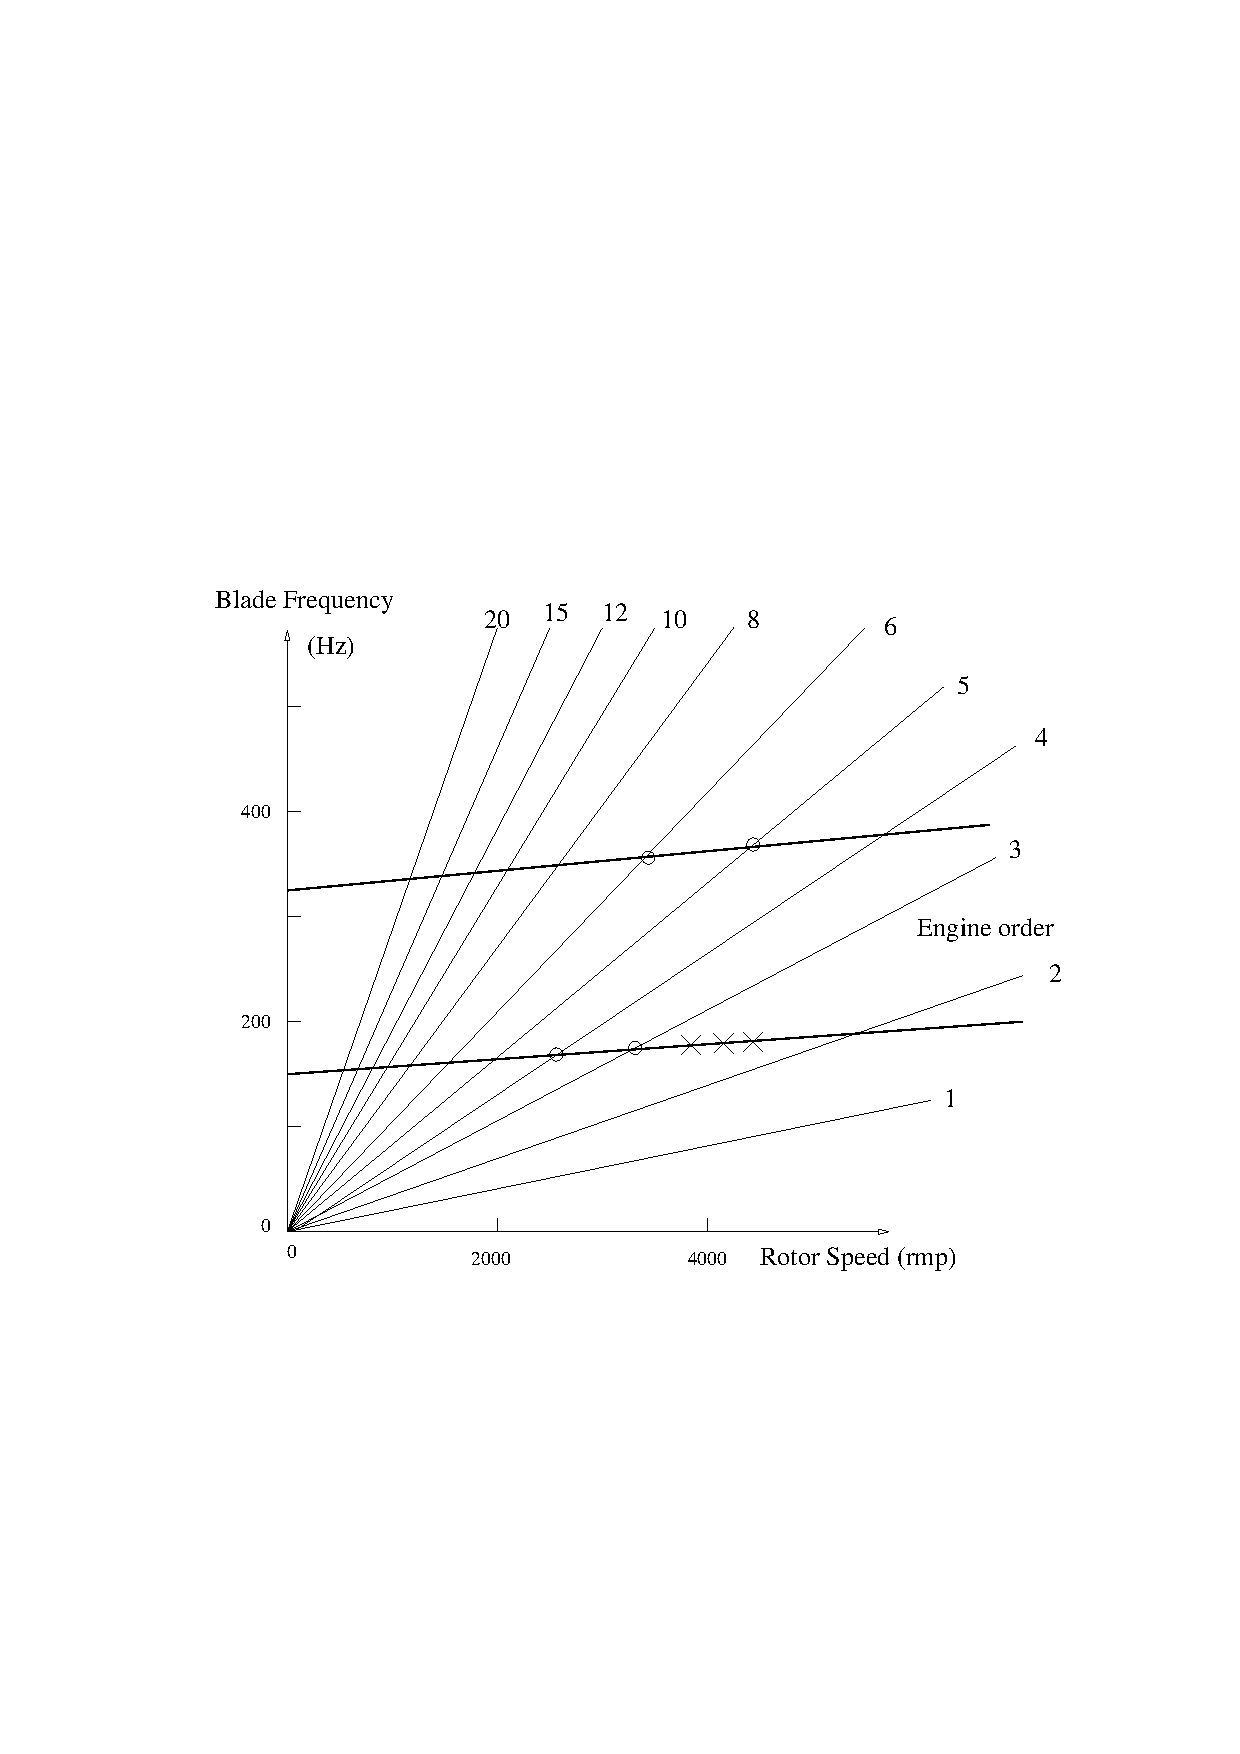
\includegraphics[width=130mm, clip=t]{CHAP_INTRO/FIGURE/campell.pdf}}
  \caption{Campbell diagram for a rotor blade (from Sisto 1987).
   x non-synchronous excitation (flutter), o forced response resonance.}
  \label{campell.fig}
\end{figure}
%
 Unfortunately, it is not usually possible to move all resonances out of the
 running range because aeroengines operate over a wide range
 of speeds and aerodynamic conditions.
 So, it is of paramount importance to be able to evaluate the unsteady
 aerodynamic loads in order to calculate the magnitude of aerodynamic
 responses for fatigue life predictions.
 This problem is usually more severe in HP turbines, where the
 blades are already under large thermal and centrifugal loading.
 Jay \& Fleeter \citeyear{Fleeter:2} give an overview of the various
 aspects of forced response investigation. An assessment of unsteady flows
 in turbines caused by the relative blade motion is given
 by Sharma et al. \citeyear{Sharma:1}.

 In aerospace engineering, it is common practice to display
 engine test results in the form of a modified Campbell diagram from
 which both flutter and forced response behaviour can be seen.
 In such cases, the out-of-plane axis represents the vibration
 amplitude and flutter is observed at nearly constant frequency,
 usually across several engine-order lines (Fig. \ref{campell.fig}).

 The main sources of unsteadiness, which can cause forced blade
 vibrations, can be due to the wake passing from upstream blade rows
 (wake-blade interaction) and the potential field of up/downstream
 blade rows.
%
\paragraph{Wake-rotor interaction.}
%
 The stator wakes, which can be
 assumed to be approximatively steady in the stator frame of
 reference, are unsteady in the rotor frame of reference since
 the rotor is moving through the wakes and, consequently, unsteady
 pressure waves are created. Although the generation of stator
 wakes is viscous phenomenon, the subsequent interaction with
 the rotor blade is primarily an inviscid process and hence can
 be modelled, as a first approximation, by the Euler equations.
 This allows two different approaches in numerical modeling.
 The first is to perform a full Navier-Stokes calculation for both the
 stator and rotor blades (Rai \citeyearNP{Rai:1,Rai:2},
 Arnone \citeyearNP{Arnone:1}. The second is to perform an unsteady
 inviscid calculation for just the rotor blade row, with the wakes
 being somehow specified as unsteady inflow boundary conditions
 (Hodson \citeyearNP{Hodson:1}, Giles \citeyearNP{Giles:2},
  Korakianitis \citeyearNP{Kora:1,Kora:2,Kora:3}).
 This latter approach is computationally much more efficient,
 but assumes that one is not concerned about the unsteady heat
 transfer and other viscous effects on the rotor blades and that the
 wake is steady in the stator frame of reference.
%
\paragraph{Potential interaction.}
%
 Such interaction cause
 unsteadiness due to the fact that the pressure in the region between
 the stator and rotor blade rows can be decomposed approximately
 into a part which is steady and uniform, a part that is
 non-uniform but steady in the rotor frame and a part that is
 non-uniform but steady in the stator frame. Therefore, as the rotor
 blades move, the stator trailing edges experience an unsteady
 pressure due to the non-uniform part that is locked to the rotors,
 and the rotor leading edges experience an unsteady pressure due to the
 non-uniform part that is locked to the stator.
 This is a purely inviscid interaction , hence the term potential interaction.
 There are again two modelling approaches:
 the first is an unsteady inviscid calculation of the stator and rotor
 blade rows (Giles \citeyearNP{Giles:3}, Suddhoo et al. \citeyearNP{Giles:11},
 Rai \citeyearNP{Rai:1,Rai:2}, Sbardella \& Peir\'{o} \citeyearNP{Luca:1}).
 The second is an unsteady inviscid calculation for just
 one of the blade rows, either the stator or the rotor, with the
 unsteady pressure being specified as boundary condition
 (Korakianitis \citeyearNP{Kora:1,Kora:2,Kora:3},
 Manwaring \& Wisler \citeyearNP{Manwaring:1}).
 The latter approach is more efficient but, unfortunately, the
 potential stator/rotor interaction becomes important
 when the spacing between the stator and the rotor is extremely small,
 and/or there are shock waves moving in the region between them.
 Consequently, one does not usually know what to specify
 as unsteady boundary conditions.
%
%
\paragraph{Low engine order (LEO) excitation.}
%
 Both wake-rotor and potential-flow interaction can be regarded
 as classical forced response problems related to blade passing frequency.
 For such forced response problems, the frequency of the excitation forces
 is a known function of the number of the up/downstream blades and the
 rotational speed.
 The second type of forced response is much more difficult to deal with as
 the controlling parameters and the exact excitation mechanisms are poorly   understood.
 However, the unsteady aerodynamic forcing function is known to be made of  low-order harmonics as it is responsible for exciting low-order nodal diameter
 assembly modes, hence the term LEO forced response.
 From an industrial perspective, the LEO forced response may be more important than
 the classical forced response as there are no established design procedures
 for its avoidance.
 Many factors, such as flow angle, rotor-stator axial gap, combustion effects,
 effects of up-downstream stages, are thought to influence the LEO
 excitation mechanism but no symmetric trends can be observed.
 Sayma \citeyear{Mehdi:4} gives an overview of different factors which may
 effect the LEO forced response.
 Manwaring \& Kirkeng \citeyear{Manwaring:2} present an investigation
 for forced response on a low pressure (LP) turbine blade row, due to low-engine
 order temperature distorsions caused by the upstream combustor.
 Sayma et al. \citeyear{Mehdi:7} predicted the LEO excitation
 arising from a stator blade throat width variations.
%
%
\subsection{Flutter}
%
 Flutter is defined as an unstable and self-excited vibration of a body in an
 air-stream and it results from a continuous interaction between the fluid and
 the structure, either or both of which may be non-linear in nature.
 Flutter is an aeroelastic phenomenon.
 Collar \citeyear{Collar:1} define aeroelasticity as the
 study of the mutual interaction that takes place within the triangle
 of inertial, elastic and aerodynamic forces on structural members exposed to
 an airstream.

 In turbomachinery blade rows, the structure to fluid mass ratio tends to be
 high while the same parameter is much lower for wings. Thus, whereas the
 wing flutter usually occurs as a result of coupling between the (bending and
 torsional) modes, turbomachinery blade flutter tends to be a single mode
 phenomenon as the aerodynamic forces, which remain much smaller than the
 inertial and stiffness ones, cannot usually cause modal coupling. In the
 former case, the aeroelastic mode can be significantly different from the
 structural one, in both frequency and mode shape, while this is usually not
 the situation in the latter case. However, there may still be discrepancies
 between the aeroelastic mode and the corresponding structural mode.
 Coupled mode turbomachinery flutter cannot be ruled out, and may occur in
 modern designs where blading tends to become thinner and more highly loaded
 to improve the aerodynamic efficiency. In any case, flutter is a particularly
 difficult problem in turbomachinery cases since there are many additional
 features with not fully-understood consequences: flow distortions due to up
 and downstream blade rows, intake effects, coupling of assembly modes,
 loss of spatial periodicity of vibration due to aerodynamic effects and
 blade-to-blade manufacturing differences,
 a feature which is known as mistuning (Ewins \citeyearNP{Ewins:1}).

 Reviews of advances in the field of aeroelasticity in turbomachine applications
 have been published by Sisto \citeyear{Sisto:4}, Fleeter \citeyear{Fleeter:1},
 Platzer \citeyear{Platzer:1}, Sisto \citeyear{Sisto:2},
 Dowell et al. \citeyear{Sisto:3}, Bendiksen \citeyear{Bendiksen:1},
 Gerolymos \citeyear{Gerolymos:1}, Marshall \& Imregun \citeyear{Imregun:1}.
%
\begin{figure}
  \centerline{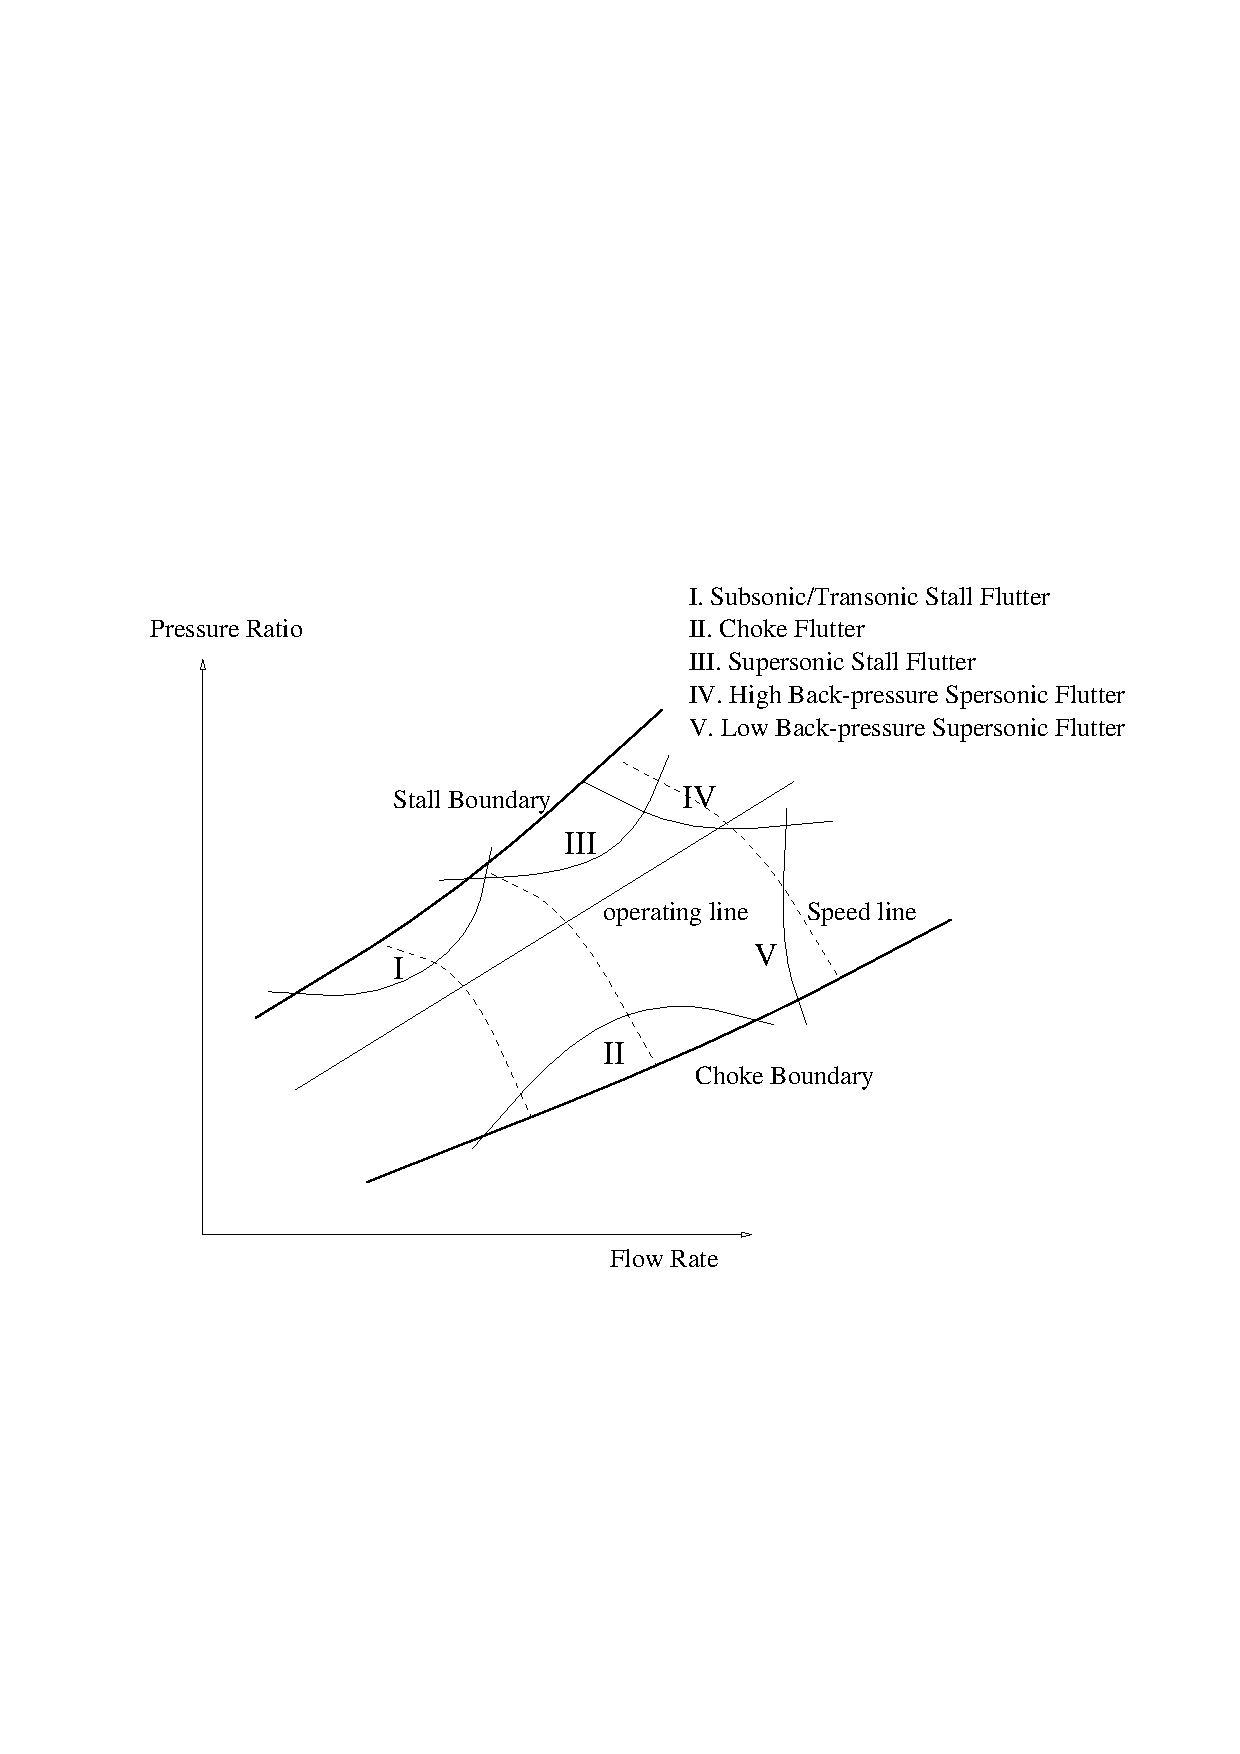
\includegraphics[width=130mm, clip=t]{CHAP_INTRO/FIGURE/fan_map.pdf}}
  \caption{Blade flutter boundaries on compressor map (from Sisto 1987)}
  \label{fan_map.fig}
\end{figure}
%

 A typical compressor map which indicates the different flutter regions
 is shown in Fig. \ref{fan_map.fig}. This map shows the various possible
 flutter regimes: stall flutter, choke flutter and various type of
 supersonic flutter.
 Sisto \citeyear{Sisto:1} gives an overview of the different types of
 flutter in modern compressor and fan. In this review paper
 particular attention as been devoted to the illustration of classical
 and modern prediction models.
%
%
%
\paragraph{Stall flutter.}
%
 As shown in Fig. \ref{fan_map.fig}, the aerodynamic conditions,
 at which stall flutter tends to occur, are at part-speed with high
 back pressure.
 In such conditions, the incidence onto the blades is high and the
 blade boundary layer becomes thicker. At transonic
 flow conditions, which are typical of front stage fans,
 a shock wave stands outside the blade passage, i.e. misses the
 leading-edge of the next blade.
 This leads to strong shock/boundary-layer interaction, which may be an
 important part of the stall flutter mechanism.
 Stall flutter differs considerably from classical flutter,
 i.e. with attached flow (Sisto \citeyearNP{Sisto:2}).
 The mechanism for net energy transfer from the airstream to an oscillating
 blade need not to rely on elastic or aerodynamic coupling between two modes,
 nor upon a phase lag between a displacement and its aerodynamic reaction.
 The essential feature of stall flutter is the non-linear aerodynamic
 reaction to the motion of the blades.
 Dowel et al. \citeyear{Sisto:3} describe a models for bending and torsional
 stall flutter including the basic instability mechanism and its principal
 features.
 Adamczyk et al. \citeyear{Adamczyk:1} present an analysis of supersonic stall
 flutter of modern fan assemblies.
%
%
%
\paragraph{Choke flutter.}
%
 Compared to stall flutter, choke flutter usually occurs at the opposite
 end of the compressor map. Here the incidence onto the blades decreases
 and becomes negative.
 At subsonic flow conditions, this may lead to the separation of the
 boundary layer from the pressure surface, and the flutter mechanism
 is similar to that of stall flutter. At transonic conditions, choke
 will normally occur before stall and large unsteady pressures
 from oscillatory shocks may cause flutter.
 Choke flutter is described qualitatively by Dowel et al. \citeyear{Sisto:3}.

~\newline
 Although low-pressure turbine stages are also known to be prone to flutter
 (Sayma et al. \citeyearNP{Mehdi:5}), fan flutter
 stability is usually considered to be more critical as this component can be
 exposed to effects such as inlet distortion due to gusts, cross-winds and
 foreign object damage. Therefore, a higher flutter margin needs to be
 incorporated into its design.
%
%
%
%
\subsection{Inherent unsteadiness}
%
 Several unsteady phenomena may result from aerodynamic instabilities
 of the fluid. Such instabilities are primarily due to the viscosity
 of the fluid and apply to both turbine and compressor blades.
 Two main aerodynamic instabilities are of concern
 in turbomachinery flows: vortex shedding and rotating stall.
%
\paragraph{Vortex Shedding.}
%
 Trailing edge vortex shedding is a major source of unsteadiness in turbomachinery
 when viscous flow exits via a blunt blade trailing-edge. This unsteadiness
 is particularly pronounced in turbines where very thick trailing-edges are
 needed to accommodate blade cooling passages.
 Some experimental works suggested that the wake loss in a turbine is
 largely due to the formation of a vortex shed.
 Unfortunately, the detailed mechanism of vortex shedding loss production
 is still not quite clear.
 One observation is that, when vortex shedding occurs,
 the total pressure just downstream of the trailing
 edge (base region) is significantly lower than that of the free-stream,
 producing a base pressure loss (Wilson \citeyearNP{Wilson:1}).
 Predicting the base pressure is an important part of predicting the loss
 produced by the vortex shedding. Because vortex shedding in turbomachines
 has a small length scale and high frequency, the experimental and numerical
 investigations are difficult and expensive. However, understanding
 and predicting trailing-edge vortex shedding
 is important to reduce the total losses further in turbine designs
 and is receiving more and more attention.
 Cicarelli \& Sieverding \citeyear{Sieverding:2} present a numerical simulation
 in order to assess the effects of vortex shedding on the unsteady pressure
 distrubution around the trailing-edge of a turbine cascade.
 Magagnato \citeyear{Magagnato:1} uses different forms of two equation
 turbulence models in order to predict the experimentallly observed vortex
 shedding from a turbine trailing edge. The results indicates a strong
 dependency on the particular turbulence model used.
 Denton \citeyear{Denton:2} discusses turbine vortex shedding in term
 of losses due to entropy generation.
%
\paragraph{Rotating stall.}
%
 Stall may occur when a compressor blade runs off design, and the incidence
 on the blade increases (above the working line in Fig. \ref{fan_map.fig}).
 As a consequence, at least three different instabilities may occur:
 the first is stall flutter, described above;
 the second is {\em surge}, where the higher pressure downstream of the stalling
 stage causes the whole flow to reverse. This
 serious system instability can cause structural damage very suddenly.
 The third instability, rotating stall, occurs when, due to differences
 in the flow around the annulus (inlet distortion or upstream obstruction)
 only some of the blades stall.
 The stalled cell then causes a higher incidence onto the blades nearest in the
 opposite direction to the rotation (causing those to stall),
 and a lower incidence onto the blades nearest in the rotating direction
 (causing those to recover).
 Thus the stalled cell rotates around the annulus in the opposite
 direction to the rotor rotation.
 This phenomenon obviously causes large unsteady forces on the blades, so at least
 some forced vibration would be expected to accompany rotating stall.
 The propagative behaviour of rotating stall was initially described by
 Emmons et al. \citeyear{Emmons:1}.
 Advances in the area of rotating stall has been reported by
 Greitzer \citeyear{Greitzer:1,Greitzer:2}, Cumpsty \citeyear{Cumpsty:1}.
%
%
%
%
\subsection{Further aspects of unsteady flows in turbomachines}
%
 There are two main parameters which are of paramount importance in
 turbomachinery unsteady flows and these are the {\em interblade phase angle}
 and the {\em reduced frequency}.
 The interblade phase angle can be associated with both flutter and forced  response problems (stator/rotor interaction). This quantity, firstly
 introduced by Lane \citeyear{Lane:1} for flutter problems,
 indicate the phase difference between vibrating neighboring blades.
 The possible values of the interblade phase angle in a flutter analysis are
 defined by
%
\beq
  \phi = \frac{2 \pi n}{N\sm{b}}
  \label{ibps_flutter}
\eeq
%
 where $N\sm{b}$ represents the number of blade in the annulus and $n$ represents
 the wave number $\left(n = 0, 1, \dots, N\sm{b}\right)$.

 For stator/rotor interaction an equivalent definition can be formulated.
 This time, the interblade phase angle is decided by the pitch ratio
 of neighboring blade rows.
 For example, for a single turbine stage shown in Fig. \ref{turbine_stage.fig},
 the stator blade row has a blade pitch given $P\sm{s} = \frac{2 \pi}{N\sm{s}}$
 and the rotor blade a pitch given by
 $P\sm{r} = \frac{2 \pi}{N\sm{r}}$, where $N\sm{s}$ and $N\sm{r}$ are
 the blade numbers.
 Assuming $N\sm{s} \leq N\sm{r}$, the interblade phase angle between
 the upper and periodic boundaries is:
%
\beq
  \phi = 2 \pi\left(1 - \frac{N\sm{s}}{{N\sm{r}}}\right)
  \label{ibps_forced}
\eeq
%
\begin{figure}[ht]
  \centerline{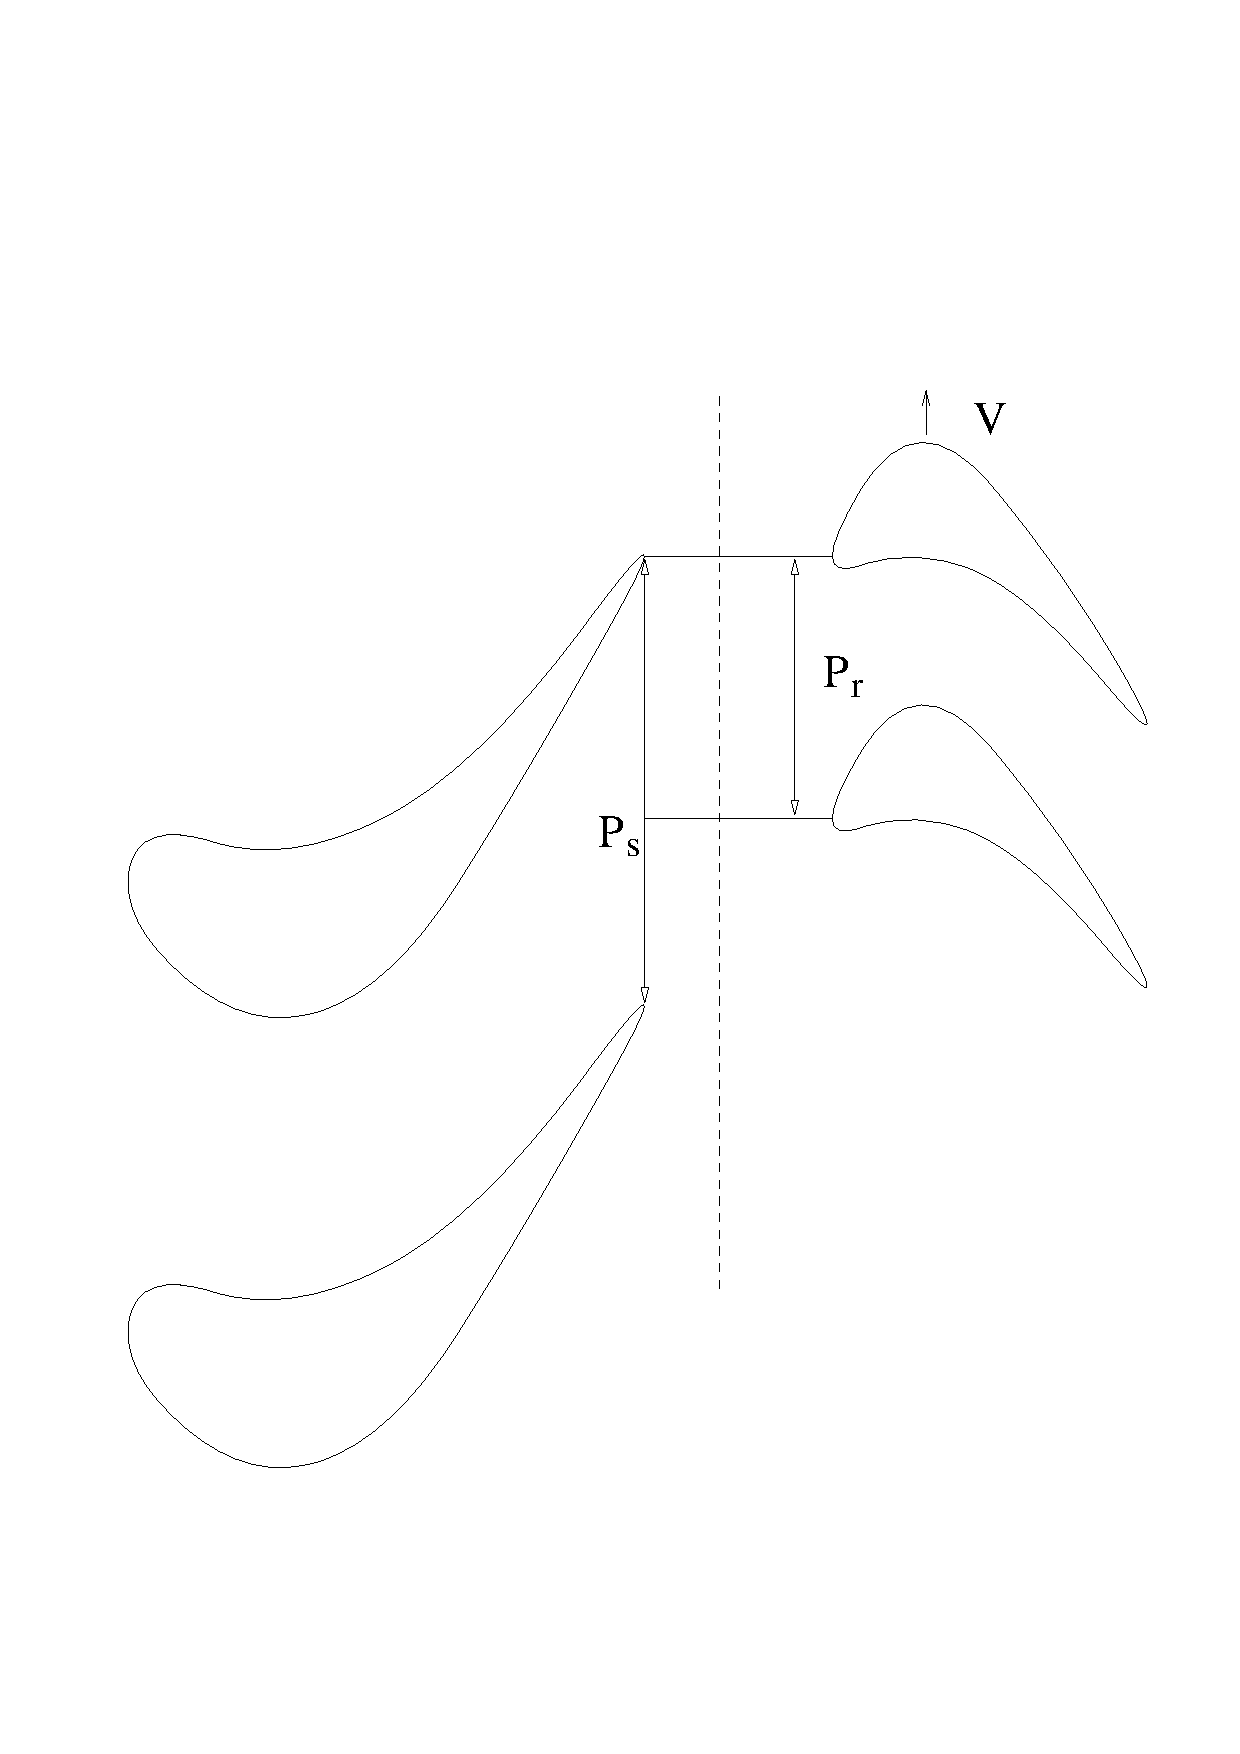
\includegraphics[width=60mm, clip=t]{CHAP_INTRO/FIGURE/turbine_stage.pdf}}
  \caption{Turbine stage with different number of blades in each row}
  \label{turbine_stage.fig}
\end{figure}
%
 The interblade phase angle determinates the number of blade passages that must
 be included in the calculations unless some other assumption
 are introduced to limit the computational domain to a single passage
 (Erdos et al. \citeyearNP{Erdos:1}, Giles \citeyearNP{Giles:2},
  Verdon \citeyearNP{Verdon:2}).

 The reduced frequency is defined in (\ref{reduced_frequency.eq}).
 For stator/rotor interaction the reduced frequency is related to the
 interblade phase angle and the relative rotation speed of the two rows as
 indicated in (\ref{frequency_rotaz.eq}).
 The reduced frequency can be interpreted as the ratio of the time taken
 for a fluid particle to go past the blade chord (or pitch) to the
 period of the flow unsteadiness. For small values
 of the reduced frequency, the flow is quasi-steady, while
 unsteady effects dominate for large values.
%

%
%
%
%
%
\section{Computational Prediction Methods}
\headb{Introduction}{Computational prediction methods}
\label{prediction_methods.sec}
%
%
 The development of numerical methods for the prediction of unsteady
 flows in turbomachinery applications has been motivated primarily
 by the need to predict, within a prescribed level of accuracy, the
 aeroelastic and aeroacoustic behaviour of the blading.
 For the numerical prediction of the flutter margins and the actual
 level of blade vibration, an unsteady aerodynamic analysis is only
 one component of an overall design prediction system. However, because
 of the complexity of the unsteady fluid dynamic environment, this
 component has generally been regarded as the one requiring the
 most research attention.

 The unsteady aerodynamic analysis which have been used in aeroelastic and
 aeroacoustic design applications was based on classical 2D subsonic
 and supersonic analysis, supplemented by a good deal of empiricism.
 This classical 2D methods are based on linearised
 flow theories which can essentially applied to lightly loaded thin
 airfoil cascades.
 Whitehead \citeyear{Whitehead:1} gives a review of these
 methods. Classical methods provide very efficient unsteady aerodynamic
 response predictions that are useful near design operating conditions,
 but they are not appropriate
 off design, where blade loading effects are important, or for transonic flows
 with embedded shock discontinuities.

 To overcame the limitations of the classical methods, the unsteady
 flow representation needed to be improved taking into account effects due to
 the blade loading and the steady state mean flow which is highly non linear.
 During the last past decade, significant advances in unsteady
 aerodynamic prediction based on CFD (Computational Fluid Dynamics)
 methodologies have been achieved.
 At the present time there are two main approaches which deal with the
 prediction of unsteady flows in turbomachines:
 i) the time linearised methods and ii) the
 fully non-linear time marching methods.
%
%
%
\subsection{Methods for linearised unsteady aerodynamics}
\label{linear_methods.subsec}
%
 These methods are based upon the assumption that the unsteadiness
 is a small perturbation about a non-linear, steady-state flow field.
 Although solutions based on these methods require significantly more
 computer time than classical solutions, the improvement in the physical modelling,
 coupled with advances in CFD solution procedures,
 are making them an increasingly attractive for aeroelastic
 and aeroacoustic design applications.
 In fact, the linearsiation of the unsteadiness
 allows the calculations to be performed using a single passage
 for any interblade phase angle.
 On the other hand, because these methods
 are all in the frequency domain, a new calculation is needed
 for each frequency considered.
 The development history of such methods is given by Verdon \citeyear{Verdon:5,Verdon:2}.

 An improvement over classical linearised inviscid flow methods was provided
 by linearised potential methods, in which the steady flow is taken to be a solution
 of the non-linear 2D full potential equation. Verdon \& Caspar
 \citeyear{Verdon:1} developed a numerical method for solving
 the linear equations that result from assuming that the unsteadiness
 is sinusoidal in time. This class of methods takes into account the blade geometry
 and loading, and remains valid at high vibration frequencies.
 Such potential methods are all for 2D flows, with the addition of
 stream-tube thickness and radius change to introduce some 3D effects.
 The complexities of extending the potential analysis to 3D flows,
 the computational cost of the standard matrix solution methods
 and the need to capture the flow details more accurately led to
 the development of linearised Euler methods.

 Hall \& Crawley \citeyear{Hall:1} developed a finite element method for
 solving the linear Euler equations in 2D, following the
 preliminary research by Ni \& Sisto \citeyear{Ni:1}.
 Hall \& Crawley \citeyear{Hall:1} predicted subsonic
 unsteady cascade flows, and used a shock-fitting technique to calculate
 unsteady shock displacements in a 2D duct.
 However, they were not able to extend the
 shock-fitting ideas to cascade geometries because shock structures
 in real turbomachines can be complex and shocks can appear
 in  unexpected locations, requiring much more ``intelligence'' of a shock fitting
 algorithm than is possible at present.
 The present area of research is therefore focused on the implementation
 of linearised 2d and 3D Euler method which use shock capturing techniques
 as those used for non-linear aerodynamics.
 Lindquist \& Giles \citeyear{Giles:1} have proven that, if correctly formulated
 and implemented, shock capturing can produce the same results as shock fitting.
 Further work with shock capturing
 techniques have been reported by Hall \& Clark \citeyear{Hall:6},
 Hall \& Lorence \citeyear{Hall:2},
 Hall et al. \citeyear{Hall:3}, Montgomery \& Verdon \citeyear{Verdon:3,Verdon:4}.

 An active area of current research is to develop linearised
 Navier-Stokes methods, including the linearisation
 of the turbulent eddy viscosity
 (Cizmas \& Hall \citeyearNP{Hall:7} and by Holmes et al.
 \citeyearNP{Holmes:1}).
 An original formulation will also be reported in this thesis.
%
%
\subsection{Non-linear time-marching methods}
\label{nonlinear_prediction_methods.sec}
%
 Although linearised analyses meet the needs of turbomachinery designers
 for efficient predictions, they cannot model
 important unsteady flow phenomena associated with finite amplitude unsteadiness
 (large shock excursion, shock-boundary layer interaction, unsteady separation etc.).
 Over the last twenty years, there has been a great deal of work on methods
 for calculating non-linear unsteady flows by time-marching methods.
 Such methods provide a very useful research tool to increase the understanding
 of unsteady flows in turbomachinery.
 However, axial gas turbine engines are multi-stage and, in a whole engine context,
 non-linear time-marching methods are prohibitively expensive for the
 foreseeable future.
 The main complicating factor, which leads to extraordinarily large computing times,
 is the problem of the periodic boundary conditions.
 While linearised methods allow calculations on a single blade passage
 for any interblade phase angle, non-linear methods needs to include in the calculations
 a number of blade passages which depends upon the interblade phase angle
 (\ref{ibps_flutter},\ref{ibps_forced})
 unless some additional assumption are made.

 The pioneering of work was by Erdos et al. \citeyear{Erdos:1} presented
 a 2D, unsteady, inviscid flow calculation of a fan stage with unequal
 pitches using a {\em phase-shifted} periodicity condition.
 For the upper periodic boundary of each blade, this condition can be expressed as:

%
\beq
  U\left(x,y,t\right) = U\left(x,y-P,t-\Delta t\right)
\eeq
%
 where the {\em time lag} $\Delta t$ is equal to the difference in pitches divided
 by the rotor wheel speed (Fig. \ref{turbine_stage.fig}).

%
\beq
  \Delta t = \frac{P\sm{s} - P\sm{r}}{V}
\eeq
%
 The values on the lower periodic line are obtained by assuming that the flow is
 periodic in time, with a period equal to the blade passing period $T = \frac{P}{V}$.
 This allows the solution domain to be restricted to a single blade passage region,
 but a large amount of computer memory is still needed to store the unsteady
 flow variables at the two periodic boundaries over an entire period.
 However, the major drawback of this method is the assumption of
 temporal periodicity.
 Hodson \citeyear{Hodson:1} modified Denton \citeyear{Denton:3} program and
 used Erdos' technique to calculate wake-rotor interactions in a low speed
 turbine. The incoming wake was specified as a boundary
 condition, allowing the calculation to be performed with only the rotor blade.
 The results showed that many phenomena associated with rotor-stator
 interactions are dominated by inviscid rather than viscous effects.
 Rai \citeyear{Rai:1} published a paper showing that stator/rotor interaction
 can be calculated using the thin-layer Navier-Stokes equations.
 This paper generated considerable interest and sparked a lot of research activity.
 However, in order to be able to perform the unsteady calculations with few blade passages,
 without using the Erdos' technique, Rai considered some simple stator/rotor pitch
 ratios such as 1:1, 2:3 or 3:4 (Rai \citeyearNP{Rai:2}).
 Further work is reported by Jorgenson \& Chima \citeyear{Chima:1},
 Giles \citeyear{Giles:3}, He \citeyear{He:1},
 He \& Denton \citeyear{He:2,He:3},
 Arnone \citeyear{Arnone:1},
 Vahdati \& Imregun \citeyear{Mehdi:3},
 Saxer \& Felici \citeyear{Saxer:1},
 Sbardella \& Peir\'{o} \citeyear{Luca:1},
 Sayma et al. \citeyear{Luca:10}.

 Giles \citeyear{Giles:2,Giles:3}, introduced the concept of
 {\em time tilting} in order to solve wake-rotor and stator-rotor
 interactions with different blade pitches without assuming that the flow
 is temporally periodic.
 In this approach, the governing equations are rewritten in time
 inclined computational coordinates.
 This method eliminates the temporal periodicity and the storage requirements
 of the phase-shifted periodicity approach by Erdos but introduces additional
 complexities into the solution procedure.
 Giles \citeyear{Giles:4} presented the numerical
 implementation of his time tilting method into
 the 2D program UNSFLO.

 However if one is interested in multistage calculations, then both
 Erdos' and Giles' simplified methods become impractical.
 As soon as there is more than one stage, there is an unavoidable problem.
 If one considers a $1\frac{1}{2}$ stage calculation in which the first and
 second stator rows have different numbers of blades with no common factor,
 then each of the second stator row blades will experience a different unsteady
 force depending in its circumferential position relative to the blades in the
 first stator row.
 There is no mathematically correct way around this problem
 (Giles \citeyearNP{Giles:13}).
 The only correct treatment is to analyse all three blade rows.
 This approach is too expensive although some early attempts have
 been made by Sayma et al. \citeyear{Mehdi:6} who
 presented the forced response analysis of a fan using the non-linear
 time marching technique of Sayma at al. \citeyear{Luca:10}. The computation
 is performed on three whole blade rows, consisting of 11 struts, 33 variable inlet
 guide vanes (VIGVs) and 26 rotor blades.
 A view of the computational mesh, which contains about 4.2 million grid points,
 is shown in Fig. \ref{threerows.fig}.
%
\begin{figure}[ht]
  \centerline{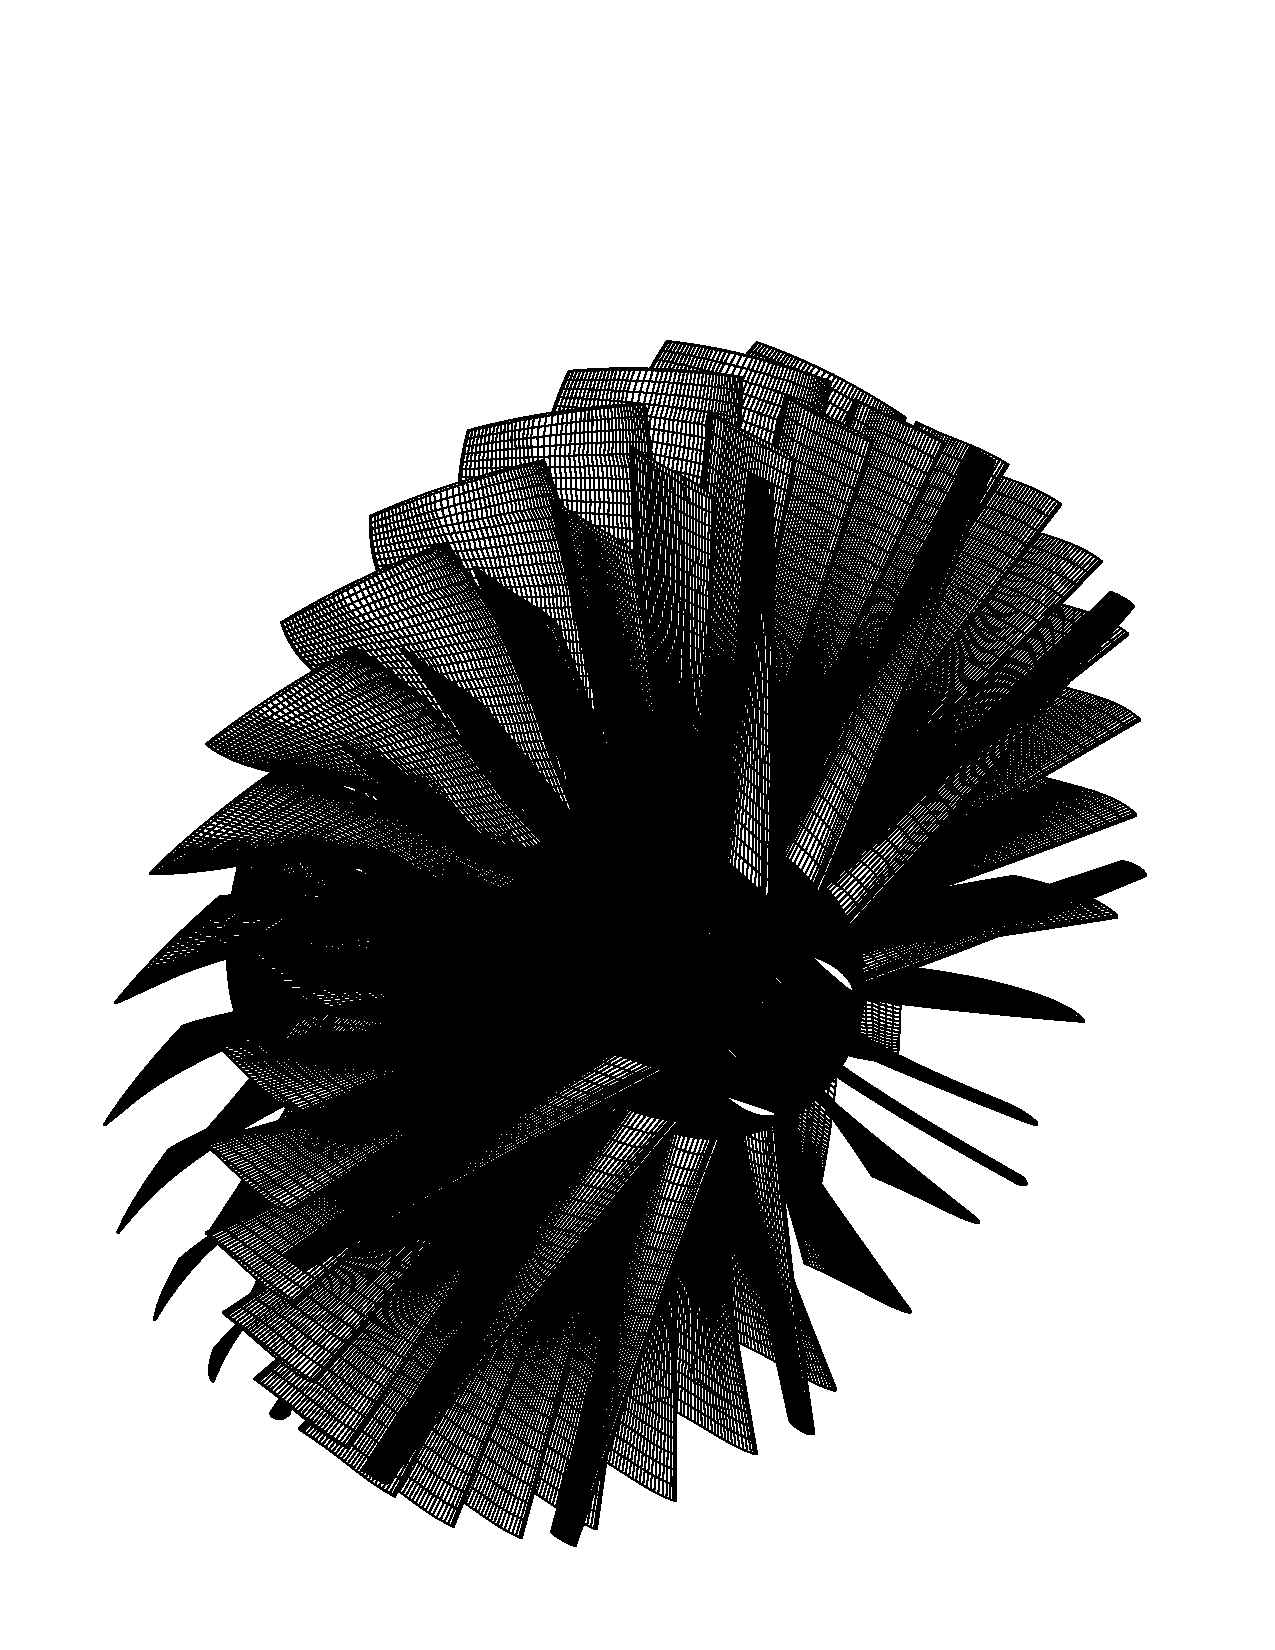
\includegraphics[width=120mm,clip=t]{CHAP_INTRO/FIGURE/threerows.pdf}}
  \caption{Three blade rows computational mesh for a 11 struts, 33 VIGVs and
           36 rotor blades (from Sayma et al. 1999)}
  \label{threerows.fig}
\end{figure}
%

%
%
%
%
%
%
\section{CFD Methods for Compressible Flows}
\headb{Introduction}{CFD methods for compressible flows}
\label{CFD_section}
%
 Both linear and non-linear unsteady flow CFD methods
 are primarily based on the solution of compressible
 inviscid or turbulent viscous flow equations.
 CFD techniques have evolved rapidly as a discipline
 and are increasingly being used to complement wind tunnels,
 both for preliminary and advanced design.
 Based on the mathematical foundations laid by Godunov \citeyear{Godunov:1} and
 Lax \citeyear{Lax:1} among others, the field has come into its own in the
 last twenty years.
 Very significant advances have been made in the areas of spatial discretisation,
 grid generation and solution strategies. Tremendous advances in computer 
 architecture and parallel processing have also contributed to the very
 rapid advances seen over the last ten years.

 When dealing with the numerical discretisation of the Navier-Stokes equations,
 several distinct issues need to be addressed. 

 i) Spatial discretisation of the inviscid fluxes.
 The system of Euler equations mathematically
 belongs to a class called {\em hyperbolic systems of conservation laws} which
 have, as their main feature, the possibility to develop discontinuities even
 when the initial data are smooth.
 This means that a numerical algorithm needs to be designed to be able to deal with
 such possibilities.

 ii) The discretisation of the computational domain with
 structured, block-structured, unstructured or mixed-element grids.

 iii) Explicit or implicit time integration.
 This represents a very broad distinction since
 several other techniques, such as preconditioning and multigrid, can be
 employed in order to accelerate convergence. 

 iv) Boundary conditions. The stability and accuracy of the numerical scheme
 may hinge on how the boundary are treated.
%
%
%
\subsection{A brief review of flux discretisation methods}
\label{flux_discretisation.sec}
%
 The accurate and efficient discretisation of the hyperbolic conservation
 laws of fluid dynamics has been studied by several authors.
 Roe \citeyear{Roe:1} developed an approximate version of the Riemann solver
 used by Godunov \citeyear{Godunov:1} in his pioneering work,
 and this approach is still one of the best numerical schemes
 for the discretisation of the Euler equations.
 The Roe scheme belongs to the class of methods called
 {\em Flux Difference Splitting} (FDS) where
 the numerical flux function is obtained through a flow decomposition into
 acoustic, entropy and vorticity waves. Each wave is
 then discretised according to its propagation speed in an upwind
 way.
 Other FDS methods have been developed by Osher \citeyear{Osher:1}, Pandolfi
 \citeyear{Pandolfi}, Harten \citeyear{Harten:2}, Leveque \citeyear{Leveque:1}
 and Einfeldt \citeyear{Einfeldt:1,Einfeldt:2}.
 
 In parallel with the FDS methods, a different class of schemes has been developed
 where the spatial discretisation is obtained using central
 differencing stabilized by an artificial dissipation term.
 Such methods, developed Beam \& Warming \citeyear{Beam:1}
 and by Jameson et al. \citeyear{Jame:1},
 are computationally more efficient then the FDS ones but their stability
 relies on the explicit addition of artificial viscosity.
 This requires the empirical determination of the so-called
 ``free parameters''.
 On the other hand, the upwind FDS method are considered to be parameter
 free.
 A third class of methods, first developed by Stager \& Warming
 \citeyear{Stager:1} and by van Leer \citeyear{Leer:5}, is known as
 {\em Flux Vector Splitting} (FVS).
 These methods introduce, in the numerical discretisation, the signs
 of the wave propagation speeds (eigenvalues of the flux Jacobian)
 but they do not attempt to solve an approximate Riemann problem.
 Different types of FVS have been developed over the last decade
 with the goal of devising an accurate numerical scheme for capturing
 shock and contact discontinuity with minimal numerical dissipation
 and oscillation.
 Among other FVS methods, it is worth mentioning the AUSM (Advection
 Upstream Splitting Method) scheme of Liou \& Steffen \citeyear{Liou:1,Liou:2},
 the CUSP (Convective Upwind Split Pressure) scheme by
 Jameson \citeyear{Jame:2,Jame:7} and the gas kinetic analogy of
 Prendergast \& Xu \citeyear{Prendergast:1}.
 
 Several authors extended the schemes above to second order accuracy
 (labelled high resolution schemes by Harten), using different mathematical
 formulations.
 Harten \citeyear{Harten:1} introduced the important concept of TVD
 (Total Variational Diminishing) to extend Roe's first order
 flux-difference scheme to second order.
 Van Leer \citeyear{Leer:1,Leer:2,Leer:3,Leer:4}
 tackled the problem in a geometric sense introducing the MUSCL schemes (Monotone 
 Upstream-centered Schemes for Conservation Laws).
 Osher \citeyear{Osher:1}, Osher \& Chakravarthy \citeyear{Osher:2}
 contributed to the mathematical foundation of these concepts and providing
 the CFD community with solid basis to simulate high-speed flows
 with shock waves and other type of discontinuity.

 One of the most spectacular outcomes of the analysis and development
 of TVD schemes is the realization that a bridge can be established
 between the upwind FDS, FVS and central discretisation schemes.
 This allows central schemes to be formulated with adapted dissipation
 satisfying TVD requirements.
 Key papers which show the relationship between central difference and
 upwind schemes are given by Swanson \& Turkel \citeyear{Turkel:1}
 and Jorgenson \& Turkel \citeyear{Turkel:2}.
 Comparisons of different numerical schemes are given by
 Woodward \& Colella \citeyear{Colella:1} and
 Swanson et al. \citeyear{Turkel:3}.
%
%
\subsection{Structured versus unstructured grid debate}
%
 The mathematical formulation of the above schemes is developed in 1D
 because the TVD analysis is not possible for multidimensional problem.
 On structured body-fitted grids, these 1D models were extended to 2D and 3D
 in a natural by using the so-called generalized coordinates.
 However, the task of generating efficient structured grids for complex
 configurations remains a serious challenge.
 The desire of computing flows over complex configurations spawned a surge of activity in the area
 of unstructured grids\footnote{The term unstructured refers to grids
 where the number of cells surrounding a typical node does not
 necessarily remain constant.}.
 The development of both structured and unstructured grid solvers will
 now be examined in some detail.
 
 In recent years, the rapid development of numerical methods for the solution
 of the flow equations and the availability of powerful computers 
 led to the emergence of various systems for the prediction of complex
 turbomachinery flows.
 Most  prediction methods for turbomachinery flows use structured
 grids (Denton \citeyearNP{Denton:3,Denton:1}, Rai \citeyearNP{Rai:1,Rai:2},
 Dawes \citeyearNP{Dawes:1},
 Arnone \& Swanson \citeyearNP{Arnone:2}, Arnone \citeyearNP{Arnone:1},
 Saxer \& Felici \citeyearNP{Saxer:1})
 On the other hand, unstructured grids received a great deal of research
 and development for external compressible flows.
 Barth \& Jespersen \citeyear{Barth:1},
 Barth \citeyear{Barth:4,Barth:2,Barth:3},
 Peraire et al. \citeyear{Peiro:2},
 Frink \citeyear{Frink:2,Frink:1},
 Mavriplis \citeyear{Mavriplis:4},
 and Venkatakrishnan \citeyear{Venkata:1} give
 overviews of the status of compressible Euler and Navier-Stokes solvers on
 unstructured grids.
 Different spatial and temporal discretisation options
 for steady and unsteady flows are discussed.

 It is only in recent years that unstructured tetrahedral grids found
 their way into 3D turbomachinery applications
 (Dawes \citeyearNP{Dawes:2,Dawes:3}, Vahdati \& Imregun \citeyearNP{Mehdi:3},
 Sayma et al. \citeyearNP{Luca:10}).
 While unstructured grid methods  provide  flexibility for discretising
 complex geometries, they have the drawback of requiring larger
 computer storage and more CPU effort than their structured counterparts.
 Due to the relatively simple shape of turbomachinery blades, structured grids
 are considered to be as the most suitable 
 route by many researchers for their discretisation.
 Design considerations increasingly require the inclusion of complex features
 such as over tip gap leakage, cooling holes in turbine blades,
 snubbered fan blades, fan assemblies with intake ducts, struts and various
 other structural elements. Due to the complexity of such geometries,
 the natural way forward is to use unstructured grids. 
 Although tetrahedral grids, the choice of which appears obvious,
 are relatively easy to generate for inviscid flow calculations and away
 from the walls for viscous flow calculations, the situation becomes more
 complicated in boundary layers, where large aspect ratio cells are
 required for computational efficiency.
 In large parts of the solution domain, the gradients normal to the walls
 are several orders of magnitude larger than those along the walls,
 thus more grid points are required  in the former direction than in the latter.
 Tetrahedral grids are not ideal for use in boundary
 layers where very small angles degrade the accuracy of the solution
 (Aftosmis et al. \citeyearNP{Aftosmis:1}).

 Such considerations led to the development of hybrid grid models
 where hexahedral or prismatic cells can be used in the boundary layers
 and tetrahedral and prismatic cells can be used to fill the domain away
 from the walls.
 The idea of using mixed elements in an unstructured mesh technique is by no means novel,
 and has been previously advocated by several authors (Barth \citeyearNP{Barth:4},
 Parthasarathy et al. \citeyearNP{Kallinderis:2}).
 In fact, many have recognized the benefits
 of mixed elements, but have nevertheless advocated the use of standard tetrahedral 
 grids, due to the homogeneity in the data structures and relative
 discretisation simplicity.
 Mavriplis \& Venkatakrishnan \citeyear{Mavriplis:3}, 
 Moinier et al. \citeyear{Giles:9} presented unified solution techniques
 which can handle mixed-elements grids.

 For turbomachinery blades, Sbardella et al. \citeyear{Luca:3,Luca:9}
 presented a method to generate hybrid semi-structured grids  
 where the boundary
 layers are filled with hexahedral cells and the rest of the domain is filled
 with triangular prisms. Such a route not only provides a very efficient
 spatial discretisation over  standard
 unstructured grids but it also provides a much better grid quality over its  
 fully structured counterparts.
 When dealing with 3D blades, the present work will use semi-structured
 grids for their computational efficiency,
 although the solver is written for general hybrid unstructured grids.
 This is achieved
 by using an edge-data structure to construct the discretisation over all
 element types.
 In this approach, the grid is presented to the solver
 as a set of node pairs connected by edges. The edge weights representing
 the inter-cell boundaries are computed in a separate preprocessor stage.
 Consequently, the solver has a unified data structure where the  
 nature of the hybrid mesh is concealed from the main calculations loops.
%
%
\subsection{Time integration using multigrid methods}
%
 Traditionally, time integration techniques may be classified into
 five groups: explicit, implicit direct method, iterative implicit
 method, preconditioning techniques and multigrid methods.
 However, some techniques can be shown to be equivalent to others 
 and state-of-the-art time-stepping algorithms combine techniques
 from several areas.
 Venkatakrishnan \citeyear{Vankata:3} gives an overview of the
 different time marching techniques for solving both steady
 and unsteady flows.
 Unstructured grid methods are compared to those used for structured,
 body-fitted grids. The convergence characteristics of
 various implicit methods are compared for a number of test cases.
 
 Explicit methods represent a straightforward way of integrating the
 system of ordinary differential equations (ODEs) which arises from the
 spatial discretisation, since they do not require any matrix inversion.
 Multistage Runge-Kutta explicit methods
 have been widely used in the CFD community (Jameson et al. \citeyearNP{Jame:1},
 Jorgenson \& Chima \citeyearNP{Chima:1}).
 The coefficients for these Runge-Kutta schemes techniques are optimised
 in order to yield a large CFL number and good damping properties
 (Jameson \citeyearNP{Jame:4}, Van Leer \citeyearNP{Leer:7}).
 Local time stepping (Jameson et al. \citeyearNP{Jame:1}, Denton \citeyearNP{Denton:3})
 and residual smoothing
 (Jameson et al. \citeyearNP{Jame:1}, Arnone \citeyearNP{Arnone:1})
 are employed to accelerate convergence.
 Even with this methodology, the convergence to steady state is usually
 unacceptably slow. For unsteady flow, multistage Runge-Kutta algorithms
 are ideal for high-frequency unsteadiness\footnote{This is the case
 of computational aeroacoustics.} where the choice of the time-step
 is not restricted by stability considerations.
 However, the may result inefficient for low-frequency unsteady flow
 and for viscous turbulent flow simulations.
 
 Implicit direct methods, in where the Jacobian matrix is directly inverted, are
 non-competitive for large problems since the matrix inversion procedure
 scales with $n\se{3}$, where $n$ is the number of unknowns
 (Venkatakrishnan \& Barth \citeyearNP{Venkata:5}).
 Moreover the governing equations are non-linear, thus a direct method cannot produce
 an answer in a single iteration and must therefore be used iteratively.

 Rather than inverting the Jacobian matrix directly at each time-step, a
 linearised system of equations may be solved at each time-step using an iterative method.
 This can substantially reduce the overall computational requirements since the
 approximate linear system need not be solved to a high degree of accuracy.
 Also, iterative methods generally exhibit lower computational complexity than
 direct inversion methods.
 In deriving the implicit system, a common practice is the use of
 a {\em defect correction procedure} which leads to a discretised
 Jacobian matrix which is a order less accurate than
 the right-hand side (Tidriri \citeyearNP{Tidriri:1},
 Mavriplis \citeyearNP{Mavriplis:5}).
 This is not only due to storage considerations and computational complexity,
 but also to the fact that the resulting lower-order matrix is better conditioned.
 However, the mismatch between the discretisation and the Jacobian operators implies
 that the resulting system is only moderately implicit.
 For unstructured meshes, the formulation of an efficient iterative technique
 can be quite complicated. For this reason, point-Jacobi iterative procedures
 have been widely used (Brenneis \& Eberle \citeyearNP{Brenneis:1},
 Anderson and Bonhaus \citeyearNP{Anderson:1},
 Sayma et al. \citeyearNP{Luca:10}).
 Slack et al. \citeyear{Slack:1}  compare the point-Jacobi,
 Gauss-Seidel and LU decomposition time integration techniques for inviscid flows
 on unstructured meshes.

 Krylov methods\footnote{A review of Krylov methods is given by
 Venkatakrishnan (1995).} represent an alternative
 to iterative methods. The general idea
 is to obtain improved updates to the solution by using information generated at
 previous updates.
 There are a number of different Krylov methods which have been developed,
 but for CFD problems the most prevalent Krylov method is the GMRES method
 (Saad \& Schultz \citeyearNP{Saad:1}).

 These classical implicit methods work relatively well for inviscid-flow
 calculation but they may prove inadequate for high Reynolds number viscous flows
 because of two reasons: (i) the need to use high aspect
 ratio cells to represent the steep gradients in the
 boundary layer regions, and (ii) the overall increase in the number
 of mesh points for practical 3D aerodynamic configurations.
 A suitable algorithm should be devised in order to take into account the
 interaction between the discretised method, the computational mesh
 and the physics of the viscous flow.
 Moreover, the right balance between the operation count,
 storage requirements and parallel scalability is also very important.
 A general solution strategy, which is suitable for devising
 efficient solution algorithms, is the multigrid approach
 (Wesseling \citeyearNP{Wesseling:1}).
 The basic idea of a multigrid strategy
 is to accelerate the rate solution convergence on a fine grid
 by using a series of coarser grids.
 
 Explicit multigrid smoothers have been widely used in the CFD community
 for solving both steady and unsteady flows. 
 A popular explicit multigrid method is the semi-discrete scheme of Jameson
 et al. \citeyear{Jame:1} which uses multi-stage Runge-Kutta time stepping
 to integrate the system of ODEs resulting from
 the spatial discretisation. Local time-stepping was also used
 in order to accelerate convergence.
 Several researchers used the technique proposed by Jameson
 et al. \citeyear{Jame:1} to obtain efficient solution procedures:
 Jameson \citeyear{Jame:4,Jame:2},
 Denton \citeyear{Denton:3},
 Mulder \citeyear{Mulder:1,Mulder:2}
 Peraire et al. \citeyear{Peiro:3},
 Mavriplis \& Martinelli \citeyear{Mavriplis:1},
 Mavriplis \& Venkatakrishnan \citeyear{Mavriplis:8},
 Mavriplis \citeyear{Mavriplis:4},
 Melson et al. \citeyear{Melson:1},
 Parthasarathy et al. \citeyear{Kallinderis:2} and
 Arnone \citeyear{Arnone:1}.

 However, despite considerable success for Euler computations,
 the multigrid approach have shortcomings for Navier-Stokes computations,
 especially high aspect ratio cells are used inside the boundary layer
 region.
 One way of decreasing the discrete stiffness caused by highly stretched cells
 is to use of a matrix time step or preconditioner.
 Recently, considerable amount of research has been devoted to the formulation
 of preconditioner multigrid algorithms for computing high Reynolds number
 viscous flows.
 Point-Jacobi preconditioners (Pierce \& Giles \citeyearNP{Giles:10},
 Pierce et al. \citeyearNP{Giles:11}) and line-Jacobi preconditioners
 (Mavriplis \citeyearNP{Mavriplis:6,Mavriplis:7}) have been reported in the
 literature.
 While point-Jacobi and line-Jacobi preconditioners are used to
 decrease the stiffness arising from the grid anisotropy in boundary layer regions,
 another class of preconditioners is also available for reducing the stiffness
 associated with low-speed compressible flows:
 Turkel \citeyear{Turkel:4,Turkel:5}, Turkel et al. \citeyear{Turkel:7},
 Van Leer et al. \citeyear{Leer:6}, Choi \& Merkle \citeyear{Choi:1}.
 An overview of modern acceleration techniques, such as preconditioned multigrid,
 is given by Mavriplis \citeyear{Mavriplis:5}.

 Appendix \ref{multigrid.chap} presents a detailed literature review of the
 current state-of-the-art multigrid techniques and develops a hybrid-grids
 Jacobi-preconditioned multigrid method for turbomachinery
 steady and unsteady flow computations.
%
%
%
%
\subsection{Non-reflecting boundary conditions}
%
 For convection dominated phenomena, such as those described by the 
 compressible Navier-Stokes equations, the formulation of correct boundary
 conditions is extremely important and its impact on the numerical scheme
 is often dominating.
 The reason for this strong influence can be traced back to the physical nature of
 the convection propagation phenomena (Hirsh \citeyearNP{Hirsch:1}).
 When obtaining a numerical solution for the Euler or Navier-Stokes
 equations, one has no choice but to truncate the computational domain.
 This is particularly true for internal flow simulations where
 the inlet/outlet boundaries are placed typically less
 than one chord away from the blade.
 For such configurations, the far-field flow contains a significant
 component of several different wave numbers, especially
 for flows which are supersonic in the flow direction but
 subsonic in the axial direction. In this case shocks propagate indefinitely
 and can be reflected by improper boundary conditions.

 The term non-reflecting boundary condition (or absorbing boundary conditions)
 indicates a far-field boundary treatment which should prevent any
 non-physical reflection of waves which are leaving
 the computational domain.
 Specialized treatments exist for steady-state flows, unsteady
 frequency-domain flows and unsteady time-domain flows.
 The milestone paper by Engquist \& Majda \citeyear{Engquist:1} reported
 a hierarchy of approximate non-reflecting boundary conditions for
 multidimensional problems. The authors constructed a non-local
 perfectly absorbing boundary condition for the scalar wave equation
 and derived highly absorbing local approximations by mean of Taylor 
 series around the incidence angle of the outgoing waves.
 The first-order approximation represents the so-called {\em 1D
 approximation}, or {\em method of characteristics},
 where only the waves which travel in the direction normal to the
 far-field boundary are perfectly absorbed.
 This approach is the most commonly used one for time-domain
 unsteady flow computations (Thompson \citeyearNP{Thompson:1,Thompson:2}).
 
 An overview of different types of non-reflecting boundary conditions
 is given by Givoli \citeyear{Givoli:1} for a large number of problems.

 Unfortunately, the paper by Engquist \& Majda \citeyear{Engquist:1}
 was written for mathematicians,
 specialized in the analysis of partial differential equations and hence
 its acceptance and implementation by the CFD community has been slow.
 Hedstrom \citeyear{Hedstrom:1} applied the 1D
 boundary conditions of Engquist \& Majda to the unsteady 1D
 Euler equations.
 Higdon \citeyear{Higdon:1} discussed the initial-boundary value problem
 theory for linear hyperbolic systems and gave a physical interpretation
 in terms of wave propagation. Furthermore, Higdon \citeyear{Higdon:2,Higdon:3} 
 formulated a discrete numerical version of the analytical absorbing boundary
 condition of Engquist \& Majda \citeyear{Engquist:1}.

 During the late 1980s, a considerable amount of manpower was devoted towards
 the formulation and implementation of accurate boundary conditions for the
 multidimensional Euler equations.
 Engquist \& Gustafsson \citeyear{Engquist:2} investigated steady-state
 non-reflecting boundary conditions and their impact on the rate of
 convergence in practical steady-state flow calculations.
 Gustafsson \citeyear{Gustafsson:1} applied Engquist \& Majda \citeyear{Engquist:1}
 theory to the 2D time-dependent Euler equations.
 For such a problem, the perfectly absorbing boundary condition
 requires first a Laplace-transform at the boundary, and then
 a Fourier-transform along in the boundary.
 Such exact non-local boundary conditions are, in a mathematical
 sense, the best possible solution of the problem. However,
 they are computationally cumbersome and they are only
 available for simple problems with constant properties.
 
 Giles \citeyear{Giles:5,Giles:6} reported a unified theory for
 the construction of steady-state and unsteady non-reflecting
 boundary conditions for the Euler equations. The analysis
 was carried out using a decomposition of the linearised Euler equations
 into Fourier modes.
 The single-frequency boundary conditions were used for
 constructing both the steady-state version (no time
 variation at steady-state, thus frequency equal to zero)
 and the unsteady frequency-domain version (single known frequency
 assumed for the unsteadiness).
 For non-linear unsteady aerodynamics, Giles constructed approximate versions
 based on Taylor expansions, similar to the formulation by
 Engquist \& Majda \citeyear{Engquist:1}.
 Giles \citeyear{Giles:6} applied the steady-state version of these boundary
 conditions to 2D turbomachinery flows, showing their effectiveness in
 avoiding numerical reflections from the computational inflow/outflow
 boundaries.
 An extension to 3D is reported by Saxer \& Giles \citeyear{Giles:7}.
 Ferm \citeyear{Ferm:1} presented accurate steady-state boundary-conditions
 for channel-flow configurations. He also studied the importance
 of a correct implementation in order to enhance convergence.

 Although accurate boundary condition formulations are now available
 to the CFD community, their application has been mainly restricted
 to steady-state flows or linearised frequency-domain unsteady flows.
 The implementation of accurate non-reflecting boundary conditions
 for time-domain unsteady flows has been reported in
 computational aeroacoustics (Tam \& Webb \citeyearNP{Tam:1}).
 For these applications, the boundary conditions are constructed from
 an asymptotic solution of the governing equations for large
 distances, the so-called {\em radiation boundary conditions}.
 A comparison between 1D characteristic
 (Thompson \citeyearNP{Thompson:1,Thompson:2}), Fourier
 decomposition (Giles \citeyearNP{Giles:5,Giles:6}) and
 radiation boundary conditions (Tam \& Webb \citeyearNP{Tam:1}),
 is given by Hixon et al. \citeyear{Hixon:1},
 in the framework of computational aeroacoustics.
 It is shown that, for unsteady time-domain 
 method, the only acceptable outflow boundary treatment is that by 
 Tam \& Webb \citeyear{Tam:1}. Other schemes become
 acceptable only in special cases when the flow is nearly
 perpendicular to the boundary.
 However, the radiation boundary conditions by Tam \& Webb \citeyear{Tam:1}
 were developed for the case of a uniform mean flow only.

 An interesting way forward could involve the use of
 the absorbing boundary conditions for linearised Euler equations
 via a perfectly matched layer (PML). This method, developed by
 Hu \citeyear{Hu:1}, uses additional computational regions adjacent to the
 far-field boundaries of the computational domain. In these regions
 the governing equations are modified so that outgoing waves are
 either damped, accelerated to supersonic conditions, decelerated
 or attenuated by combinations thereof.
 Analysis and applications of such sophisticated boundary conditions
 can be found in Tam et al. \citeyear{Tam:1}, Hesthaven \citeyear{Hesthaven:1}
 and Abarbanel et al. \citeyear{Hesthaven:2}.

%
%
%
%
%
%
\section{Objectives}
\headb{Introduction}{Objectives}
\label{objective.sec}
%
 This thesis deals with the development and application of a numerical
 tool for the simulation of unsteady turbomachinery flows for forced response
 predictions. The main goal is not only to produce a method suitable
 for industrial design but also to explore its bounds of applicability to
 practical cases.
 Both linear and non-linear time-marching unsteady flow models 
 have been implemented using an advanced finite volume algorithm on
 unstructured meshes.
 The research code, called ALiNNS (Advanced Linear-Nonlinear Navier-Stokes code),
 uses state-of-the-art CFD techniques for both spatial discretisation and temporal
 integration of the governing flow equations. The main features
 of the methodology are the use of mixed-element grids (also called hybrid grids)
 and a preconditioned agglomeration multigrid.
 Moreover a semi-unstructured mesh generator, LEVMAP (LEVel MAPping), was developed in order
 to exploit the optimum discretisation features of such an approach on 3D
 turbomachinery passages.
 LEVMAP and ALiNNS were used to predict the unsteady pressure fluctuations,
 due to relative blade rotation, on a typical HP turbine stage.
 The analysis was carried out using both linearised and non-linear aerodynamics.
 Comparisons with experimental data were made
 in order to assess the validity and the range of applicability of the linear
 method.

 The main objectives of the research project can be summarised as follow:
%
\begin{itemize}
%
\item
 The development of a semi-structured mesh generator for an efficient representation
 of 3D turbomachinery blades.
%
\item
 The development of an efficient viscous flux discretisation algorithm for
 mixed element grids and of a preconditioned agglomeration multigrid for
 efficient time integration.
%
\item
 The development of a 3D linearised viscous unsteady flow model.
%
\item
 The application of the developed non-linear and linearised flow models
 to a representative case in order to asses the applicability bounds
 of the linearised methodology.
%
\end{itemize}
%
%
\section{Contributions of the Thesis}
\headb{Introduction}{Contributions of the thesis}
\label{contributions.sec}
%
\subsection{CFD methods}
 The main contributions are summarised below.
%
\paragraph{Semi-structured meshes.}
%
 The discretisation methodology uses a combination of structured and unstructured meshes,
 the former in the radial direction and the latter in the axial and tangential
 directions in order to exploit the fact that blade-like structures
 are not strongly 3D since the radial variation
 is usually small. Such a formulation was found to
 have a number of advantages over its structured counterparts.
 There is a significant improvement
 in the smoothness of the grid-spacing and in capturing
 particular aspects of the blade passage geometry. It was also found that
 the leading- and trailing-edge regions could be  discretised without generating
 superfluous points in the far field and that further refinements of the mesh  
 to capture wake and shock effects were relatively easy to implement.
 The methodology is reported by Sbardella at al. \citeyear{Luca:3,Luca:9}
 and Sbardella \citeyear{Luca:5}. A detailed description is given in
 Chapter \ref{mesh.chap}.
%
\paragraph{Hybrid-grid flow-solver.}
%
 Compared with their structured counterparts, standard unstructured grid
 solvers have lower computational efficiency in terms of speed and storage.
 Unstructured grids often use tetrahedral elements only,
 an approach which often leads to numerical problems when the region to be discretised
 has a preferred direction such as the boundary layer for a
 high-Reynolds number flow. However, there are no fundamental difficulties in 
 extending tetrahedral meshes to include further element types such as triangular prisms,
 pentahedra and hexahedra.
 Although both the discretisation of the computational domain and the flow solver
 will become more complex,  such a mixed-element approach will offer
 a better, more efficient approximation than using tetrahedral elements only.
 For instance, hexahedral elements will handle boundary layer flows much better
 than tetrahedral elements because they can be made very slender without
 creating excessively small or large internal angles. 
 In order to handle mixed-element meshes, the spatial discretisation
 of the governing equations needs to be formulated in such a way
 that the numerical algorithms can be applied in a uniform way to all
 element types.
 Chapter \ref{flow_model.chap} describes the development and application
 of a finite volume scheme for the solution of the
 Favre-averaged Navier-Stokes equations on mixed-element grids, consisting
 of triangles and quadrilaterals in 2D, and of tetrahedra, pyramids, 
 triangular prisms and hexahedra in 3D.
 Some of the findings have already been reported in
 Sayma et al. \citeyear{Luca:10}.
%
%
\paragraph{Edge-data Laplacian weight.}
%
 A novel feature of the spatial discretisation employed in
 the ALiNNS flow solver is the use of a edge-data based Laplacian weight.
 This Laplacian weight is used to compute the Laplacian terms of the
 viscous fluxes and it results in a nearest neighbour stencils.
 Chapter \ref{flow_model.chap} describes how to evaluate the Laplacian weight
 for mixed-element meshes using an approximation of the
 Galerkin finite volume {\em node-pair} formula.
 The findings are also reported in Sbardella \& Imregun \citeyear{Luca:7,Luca:11}.
%
%
\paragraph{Preconditioned Multigrid.}
%
 A preconditioned directional-implicit agglomeration multigrid method
 has been developed for the solution of the linear and non-linear
 Navier-Stokes equations on highly anisotropic 2D and 3D unstructured hybrid grids.
 The coarse grid levels are constructed
 automatically from the fine grid by agglomerating fine grid control
 volumes together. Since the coarse grid control volumes may have arbitrary
 polygonal shapes, the type of elements constituting the fine grid is
 irrelevant. The discrete equations on coarse grid levels
 are assembled automatically without the explicit creation of a coarse grid.
 The multigrid smoother consists of a preconditioned
 point- or line-Jacobi Runge-Kutta relaxation algorithm, which guarantees
 efficient damping of high-frequency error modes on highly stretched grids.
 Appendix \ref{multigrid.chap} gives a literature review of preconditioned
 multigrid methods and describes the actual multigrid algorithm that is
 implemented in ALiNNS.
%
% 
%
\subsection{Understanding of unsteady flows}
%
 Chapter \ref{rt27.chap} presents a detailed  numerical analysis of a stator-rotor
 interaction in the case of typical HP turbine stage
 using both linear and non linear unsteady flow representations.
 The main contributions are summarised below.
%
\begin{itemize}
%
\item
 Detailed analysis of the rotor steady-state flow with discussion
 of secondary and tip leakage flow.
%
\item
 Calculation of the aerodynamic forcing functions from the
 stator outlet steady-state solution. These forcing functions
 are obtained splitting the non-linear steady-state flow
 into potential and vortical components using the theory
 reported in Appendix \ref{waves.chap}.
%
\item
 Analysis of the distinct influence of potential and vortical forcing functions
 on the rotor unsteady aerodynamics using a time-linearised approach.
%
\item
 Assessment of the predicted results by comparing them with
 experimental data and predicted non-linear results.
%
\end{itemize}
%

%
%

%
%
%
%
%
\chapter{Semi-structured Mesh Generator for Turbomachinery Blades}
 \label{mesh.chap}
\heada{Semi-structured Mesh Generator}
\setcounter{footnote}{0}
%
\newcommand{\fdx}[1]{\frac{\partial }{\partial {#1} }}
\newcommand{\fpa}[3]{\frac{\partial {\mathbf{#1}}_{#2} }{\partial {#3} }}
\newcommand{\spd}[2]{\frac{\partial^2 {#1} }{\partial {#2}^2 }}
\newcommand{\sxd}[3]{\frac{\partial^2 {#1} }{\partial {#2} \partial {#3} }}
%
%
 This chapter describes the development of a novel
 mesh generator for the flow analysis of turbomachinery blades. The
 proposed method uses a combination of structured and unstructured meshes,
 the former in the
 radial direction and the latter in the axial and tangential
 directions in order to exploit the fact that blade-like structures
 are not strongly 3D since the radial variation
 is usually small. The proposed semi-structured mesh formulation was found to
 have a number of advantages over its structured counterparts.
 There is a significant improvement
 in the smoothness of the grid-spacing and in capturing
 particular aspects of the blade passage geometry. It was also found that
 the leading- and trailing-edge regions could be  discretised without generating
 superfluous points in the far field and that further refinements of the mesh
 to capture wake and shock effects were relatively easy to implement.
%
%
%%%%%%%%%%%%%%%%%%%%%%%%%%%%%%%%%%%%%%%%
%%%%     INTRODUCTION
%%%%%%%%%%%%%%%%%%%%%%%%%%%%%%%%%%%%%%%%
%
%
\section{Introduction}
\headb{Semi-structured Mesh Generator}{Introduction}
%
 It is well known that the grid structure must be selected carefully
 in order to achieve an accurate resolution of complex flow fields
 typical of axial-flow turbomachines.
 The minimization of skewness and the optimization of smoothness
 generally result in a faster convergence as well as less solution dependence
 on the grid density, therefore reducing
 computational cost both in terms of memory and CPU time.
 As a consequence, the grid generation procedure should be considered
 an integral part of the numerical method.

 When performing a numerical simulation of turbulent-viscous flow in turbomachinery
 passage, the following aspects are of importance: i)
 accurate leading- and trailing-edge flow descriptions, ii) wake resolution,
 iii) proper gridding in the throat area where most of the shock
 is expected to occur, and iv) imposition of periodicity.

 Historically, mesh generation techniques for turbomachinery blades use
 structured hexahedral representations, the most commonly
 used ones being H-type, C-type, and O-type. These meshes are obtained either
 by using an algebraic approach (Kallinderis \& Ward \citeyearNP{Kallinderis:1})
 or by solving a system of elliptic
 partial differential equations (Thompson et al. \citeyearNP{Ellipt1},
 Steger \& Sorenson \citeyearNP{Ellipt2}, Brackbill \& Saltzman
 \citeyearNP{Ellipt3}) or by solving hyperbolic partial differential equations
 (Steger \& Chaussee \citeyearNP{Ellipt4}).
 H-type meshes have been by far the most common choice in turbomachinery
 applications as they are very easy to generate, the imposition of
 periodicity is straightforward and the mesh density before, inside,
 and after the blade passage can be easily controlled. However,
 the leading- and trailing-edge descriptions are poor and a large
 amount of superfluous points is generated in the region between
 the inflow and the leading-edge. A classical H-mesh for a transonic blade
 is shown in Fig. \ref{Hmesh.fig}.
%
\begin{figure}[ht]
  \centerline{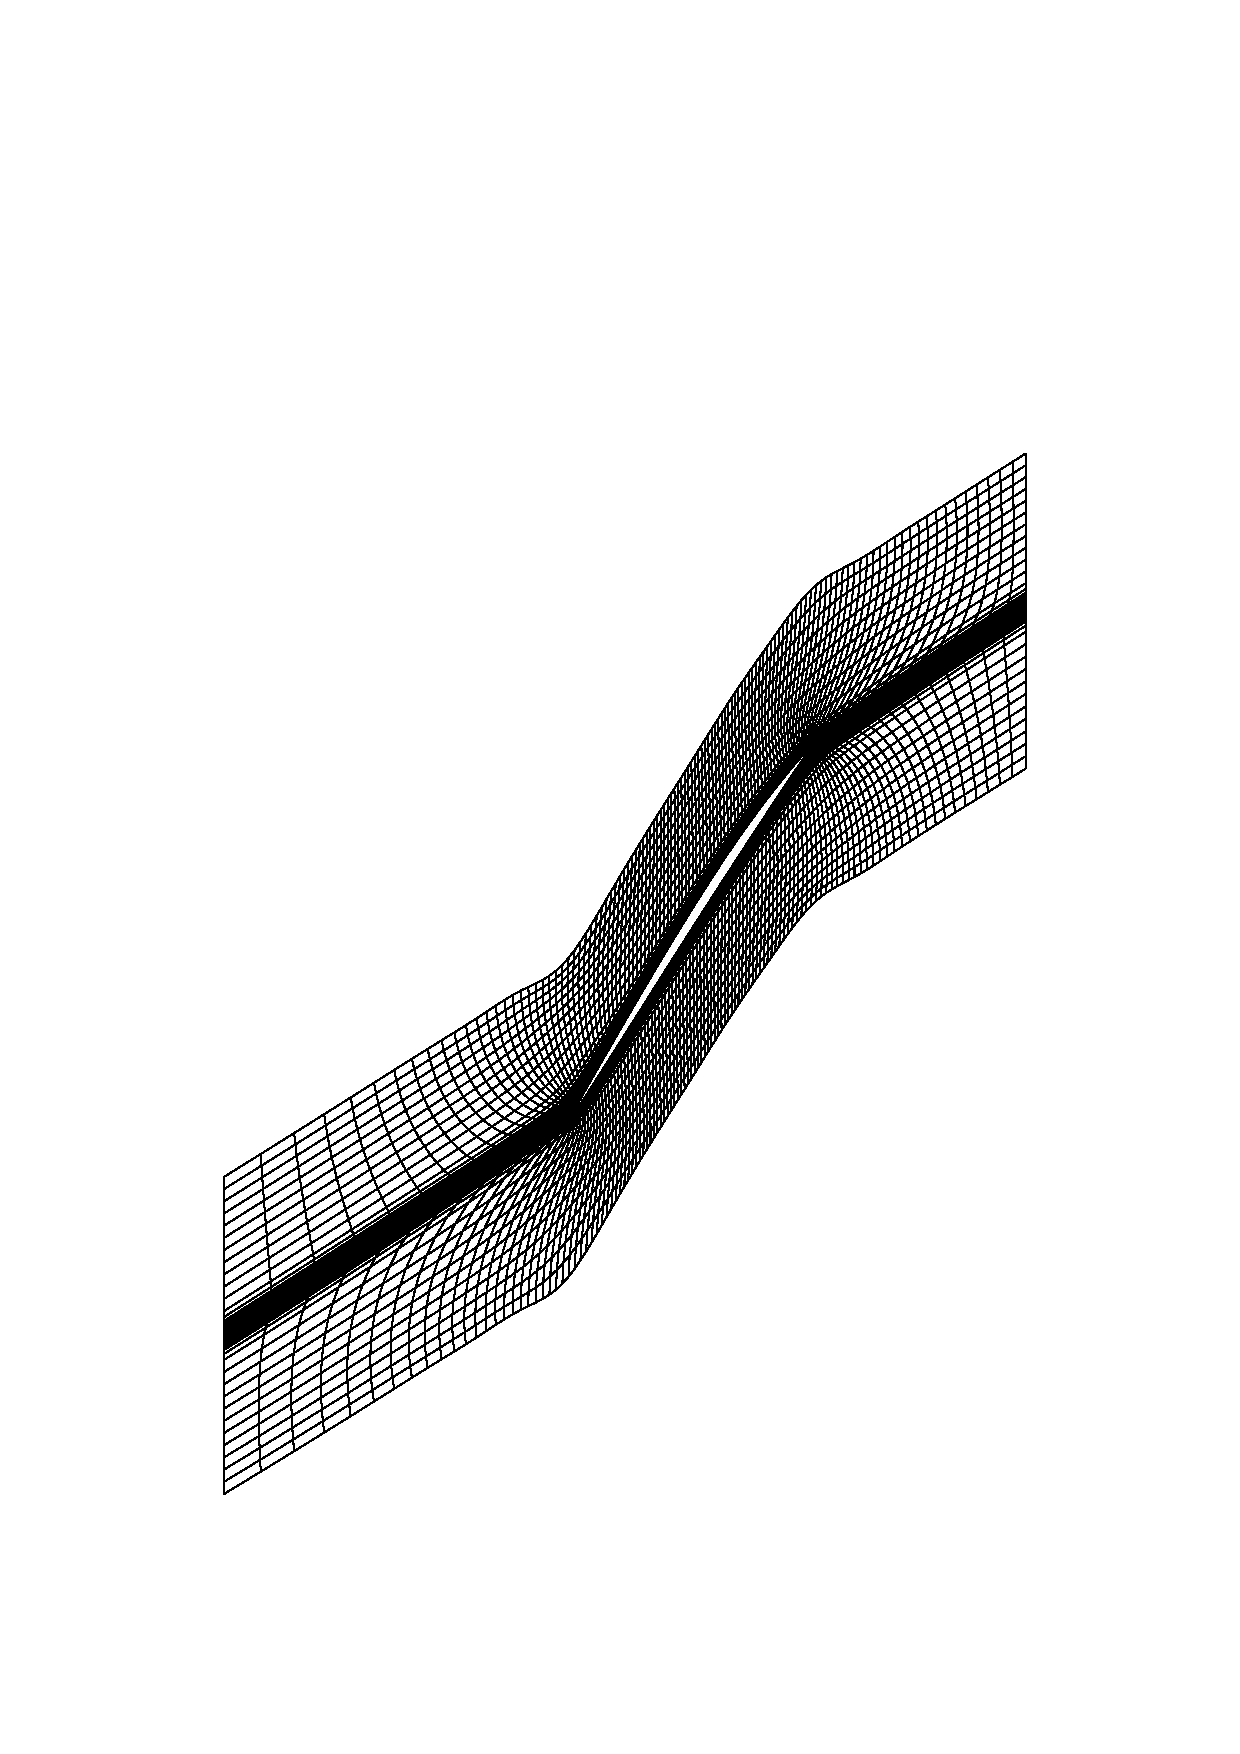
\includegraphics[width=50mm,clip=t]{CHAP_MESH/FIGURE/Hmesh.pdf}}
 \caption{Typical structured H-mesh for a fan blade geometry}
 \label{Hmesh.fig}
\end{figure}
%
 O-type grids are not very effective in capturing the wake and their
 quality outside the passage is very poor. This can smear
 the bow shock away from the leading edge of a transonic compressor
 or the outgoing shock of a transonic turbine blade.
 On the other hand, C-type meshes can capture the wake structure if
 they are carefully generated but their quality in the region between
 the inflow and the leading-edge is not suitable to resolve bow shock
 accurately.

 A different approach is to use unstructured triangular meshes
 for 2D turbomachinery calculations. Fully unstructured grids
 offer good flexibility and most of the flow features can be captured with
 good accuracy via mesh refinement.
 3D unstructured meshes are widely used in external aerodynamics but
 they have rarely been applied to turbomachinery cases.
 The main difficulty associated with such meshes is their isotropic
 nature. The very fact that tetrahedral unstructured meshes do not exhibit
 any preferred direction is what makes them ideal for discretising arbitrarily
 complex configurations. In fact most of the unstructured mesh generation
 techniques rely on this property.
 However, when a configuration with a preferred direction, such as a
 turbomachinery blade, is to be discretised,
 and different resolutions  are desired in the various directions, unstructured mesh
 generation techniques are known to experience great difficulties in
 meeting such requirements. Turbomachine blades require high resolution near
 their leading and trailing edges and radial spacing can be relatively coarse.
 When using an isotropic unstructured mesh,
 the high leading and trailing edge resolution requirements also result in
 a high radial resolution in these areas, a feature greatly increases the
 number of grid points. Such a degree of radial resolution is superfluous,
 since the radial gradients are known to be relatively small for turbomachinery
 blade flows.
 Similar difficulties occur in the boundary layer regions near a wall for
 high Reynolds number viscous flows, where the normal gradients are several
 orders of magnitude grater than the stream-wise gradients.
 To illustrate the unsuitability of unstructured meshes
 for such applications, a fully unstructured mesh was created for fan blade
 geometry using an advancing front technique (Morgan et al. \citeyearNP{Peiro:1}),
 the suction side being shown in Fig. \ref{unstruct.fig}.
%
\begin{figure}[ht]
   \centerline{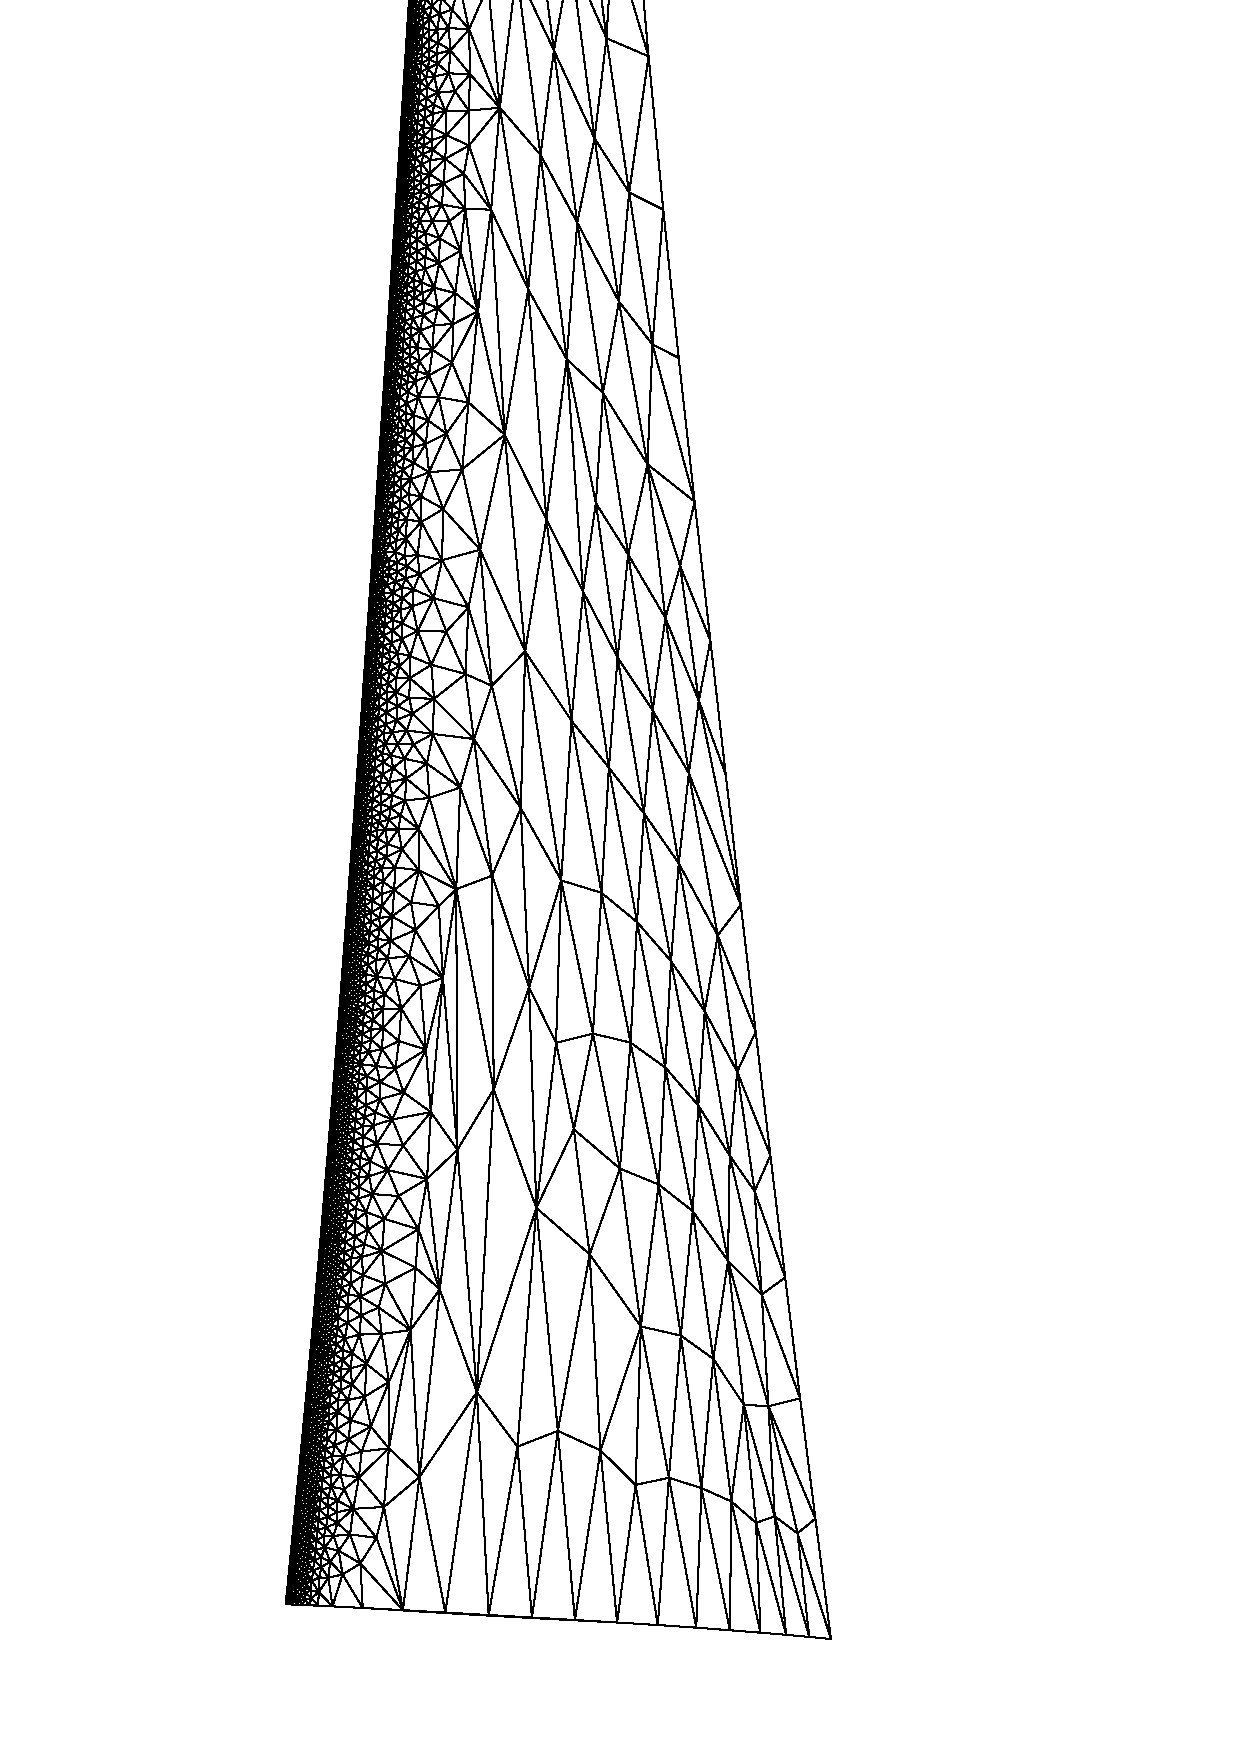
\includegraphics[width=30mm,clip=t]{CHAP_MESH/FIGURE/unstruct.pdf}}
   \caption{Fully unstructured mesh on suction surface}
   \label{unstruct.fig}
\end{figure}
%
 It is clearly seen that a large number of points are needed in the leading
 edge area in order to satisfy the resolution
 requirements, a feature which creates an unacceptably high overhead
 in the total number of points. It should also be noted that, for
 this particular geometry, the generation of an efficient viscous mesh
 will be very difficult using a totally unstructured grid because of the
 boundary layer considerations.

 The considerations above lead to the use of semi-structured meshes
 for turbomachinery blades. The aim of this chapter is to present a
 novel approach for discretising turbomachinery blades by using a combination
 of structured and unstructured meshes, the former in the radial direction
 and the latter in the axial and tangential directions.
 The basic idea relies on the fact that blade-like structures
 are not strongly 3D since the radial variation
 is usually small.
 It is therefore possible to start with a structured
 and body-fitted 2D O-grid around a given aerofoil section
 to resolve the boundary layer.
 This core mesh is then extended in an unstructured
 fashion up to the far-field boundaries,
 the triangulation being performed using an advancing
 front technique (Morgan et al. \citeyearNP{Peiro:1},
 Mavriplis \citeyearNP{Mavriplis:2}).
 Once this 2D grid is generated, it is projected to the remaining radial
 sections via quasi-conformal mapping techniques.
 When all such radial sections are formed, a 3D
 prismatic grid is obtained by simply connecting the corresponding
 points of different layers. In this way, hexahedral
 elements are generated in the viscous region and
 triangular prisms in the rest of the solution
 domain. Again, such an approach presents a distinct advantage over
 totally unstructured grids which are usually confined to tetrahedral
 elements only, though this limitation is usually a consequence of the
 unavailability of general viscous mesh generators.
%
%%%%%%%%%%%%%%%%%%%%%%%%%%%%%%%%%%%%%%%%
%%%%     GENERATION OF PRISMATIC GRID
%%%%%%%%%%%%%%%%%%%%%%%%%%%%%%%%%%%%%%%%
%
\section{Generation of Prismatic Grid}
\headb{Semi-structured Mesh Generator}{Generation of Prismatic Grid}
\label{generation}
%
 The Section is focused on the proposed semi-unstructured mesh generator
 which has six main stages:

%
\begin{itemize}
 \item Projection of all radial levels, which define the blade geometry,
       into 2D parametric planes, using local
       coordinates.
 \item Generation of a 2D unstructured hybrid-mesh for
       a given projected radial level, the so-called master plane.
 \item Generation of a coarse body-fitted structured mesh for
       all projected radial levels, including the master plane.
 \item Inverse mapping of the unstructured hybrid-mesh
       into the structured one in the master plane.
 \item Direct mapping to obtain the final unstructured mesh at all radial levels.
 \item Inverse projection of all unstructured meshes into the original
       3D radial levels.
 \item Generation of 3D prismatic grid by connecting the corresponding points
       at consecutive radial levels.
\end{itemize}
%
%
\subsection{Geometry modelling}
\label{geometry_modelling.sec}.
%
 Turbomachinery blade geometry is usually defined at a number of
 radial levels.
 In the general case, these radial levels will lie on 3D
 surfaces $\sigma_i(x,r,\theta)$, where $i$ indicates the section index, and
 $r, \theta$ are the polar coordinates. Using parametric coordinates $u$ and $v$,
 a typical surface can be defined as:

%
\beq
  \sigma_i(x,r,\theta) =
  \left\{
  \begin{array}{lll}
    x_{\sigma}      &=& x(u,v)\\
    r_{\sigma}      &=& r(u,v)\\
    \theta_{\sigma} &=& \theta(u,v)
  \end{array}
  \right.
  \label{surface}
\eeq
%
\begin{figure}
 \begin{center}
  \begin{tabular}{cc}
    \subfigure[Hub section]
      {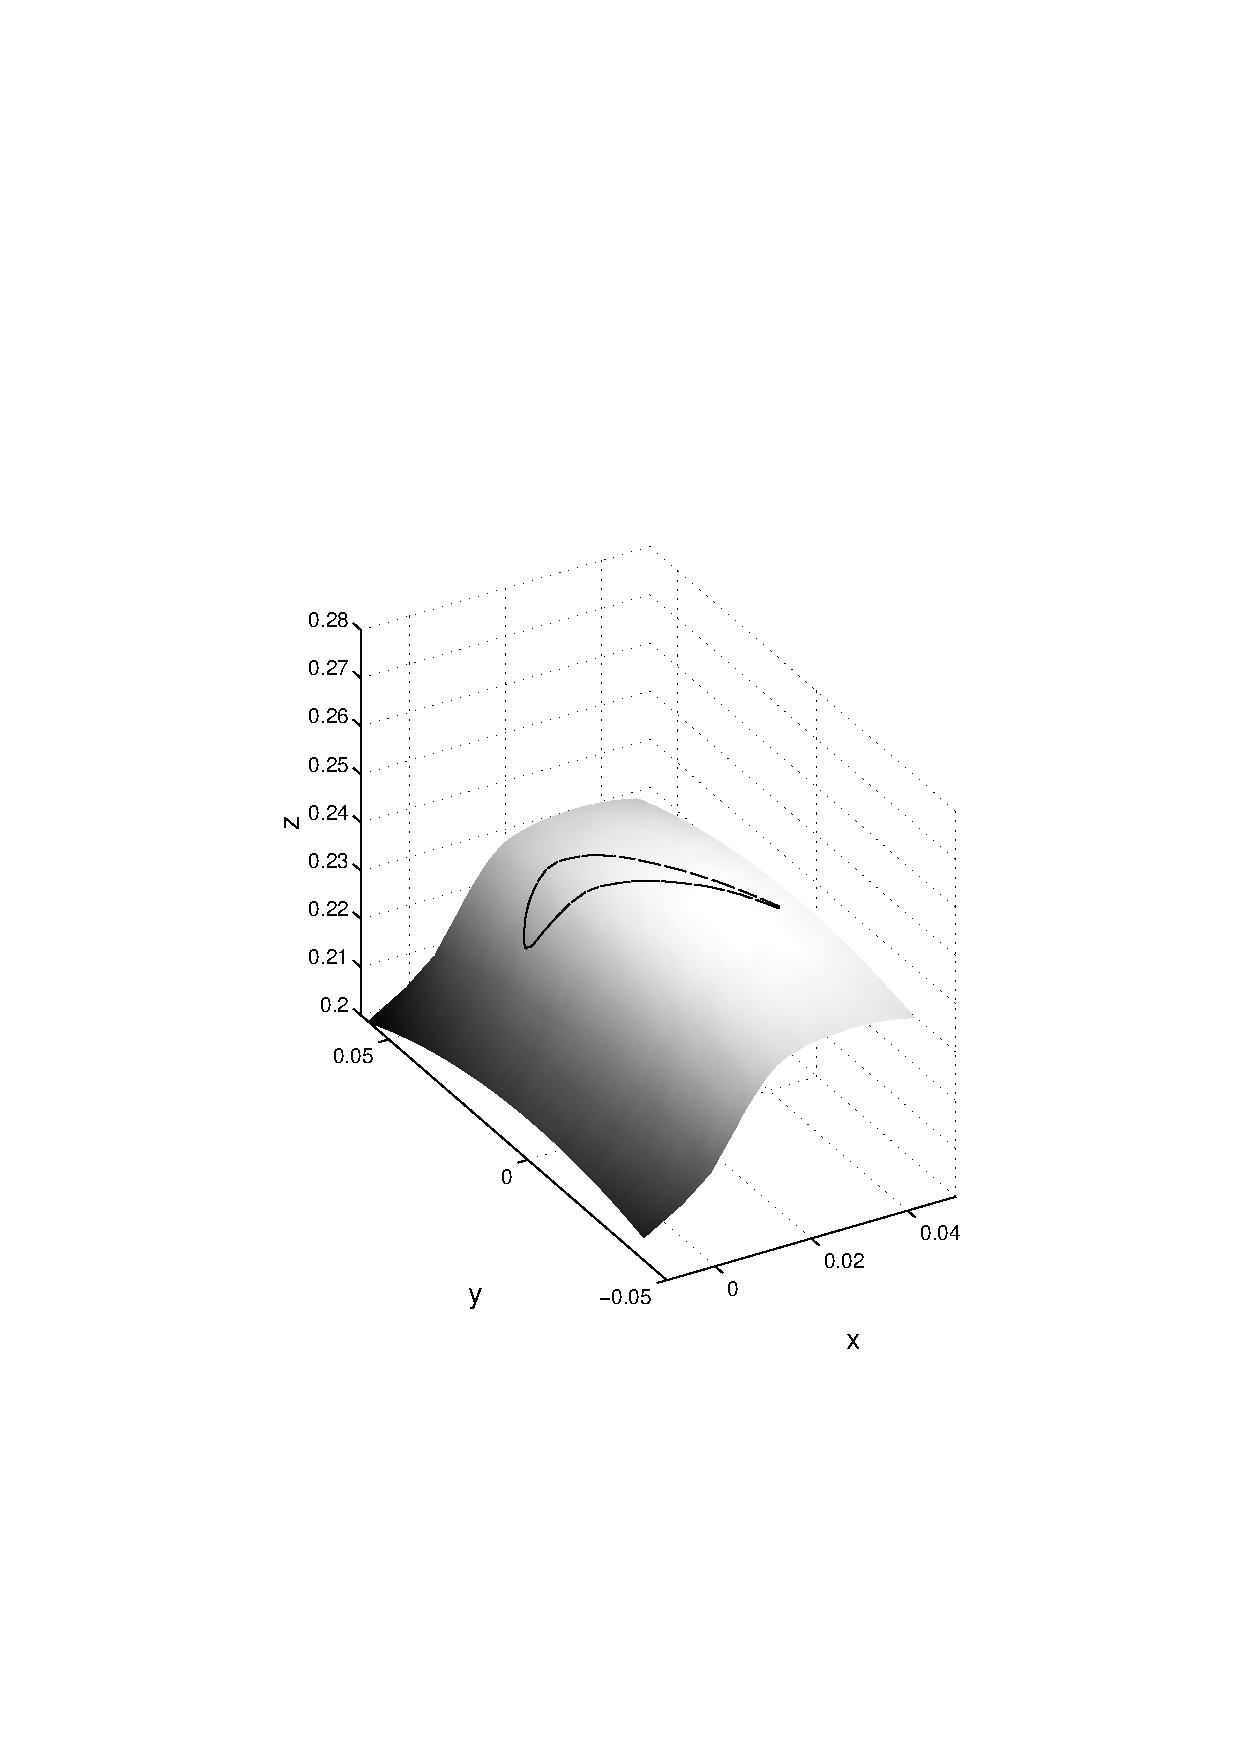
\includegraphics[width=70mm,clip=t]{CHAP_MESH/FIGURE/surf1.pdf}
      \hspace{0mm}}
    \subfigure[Hub-middle section (25\% span)]
      {\hspace{0mm}
       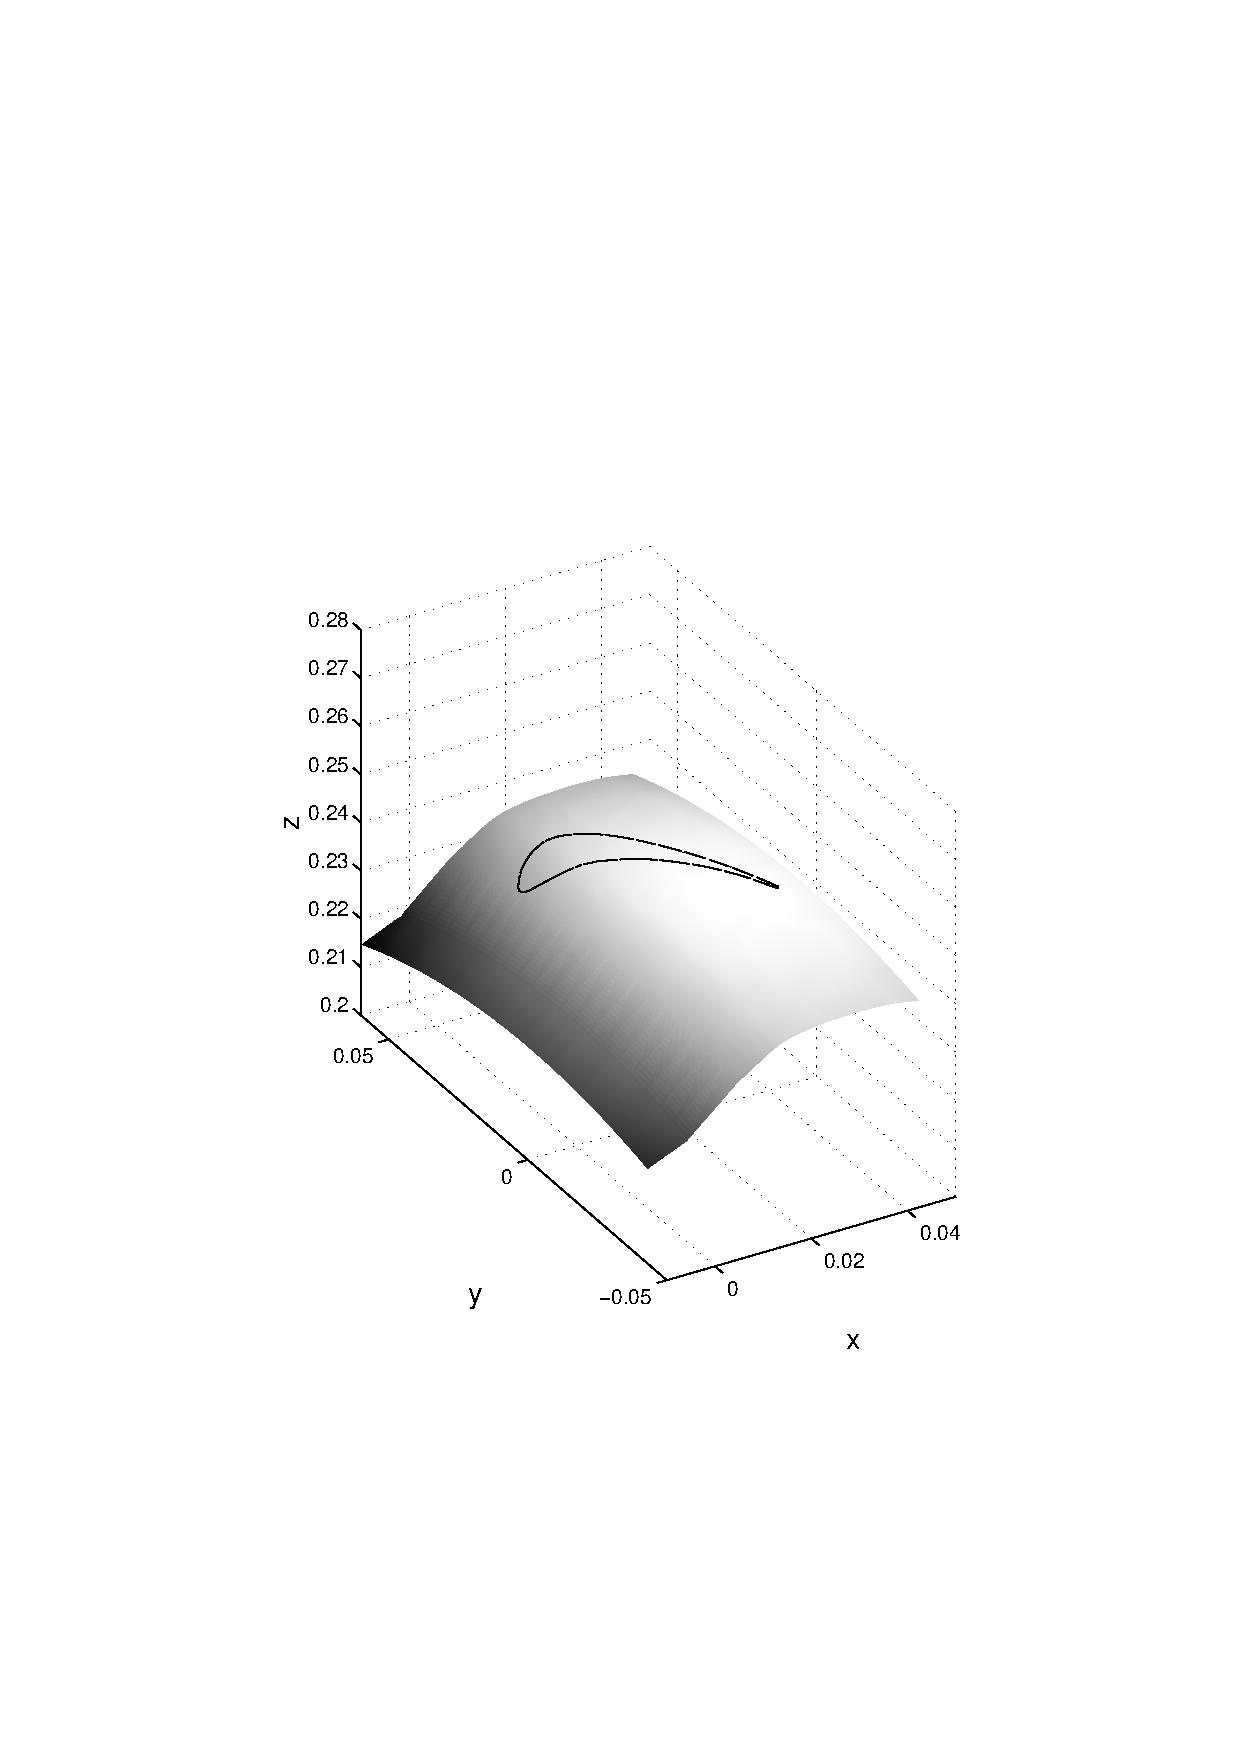
\includegraphics[width=70mm,clip=t]{CHAP_MESH/FIGURE/surf2.pdf}}
    \\
    \subfigure[Tip-middle section (75\% span)]
      {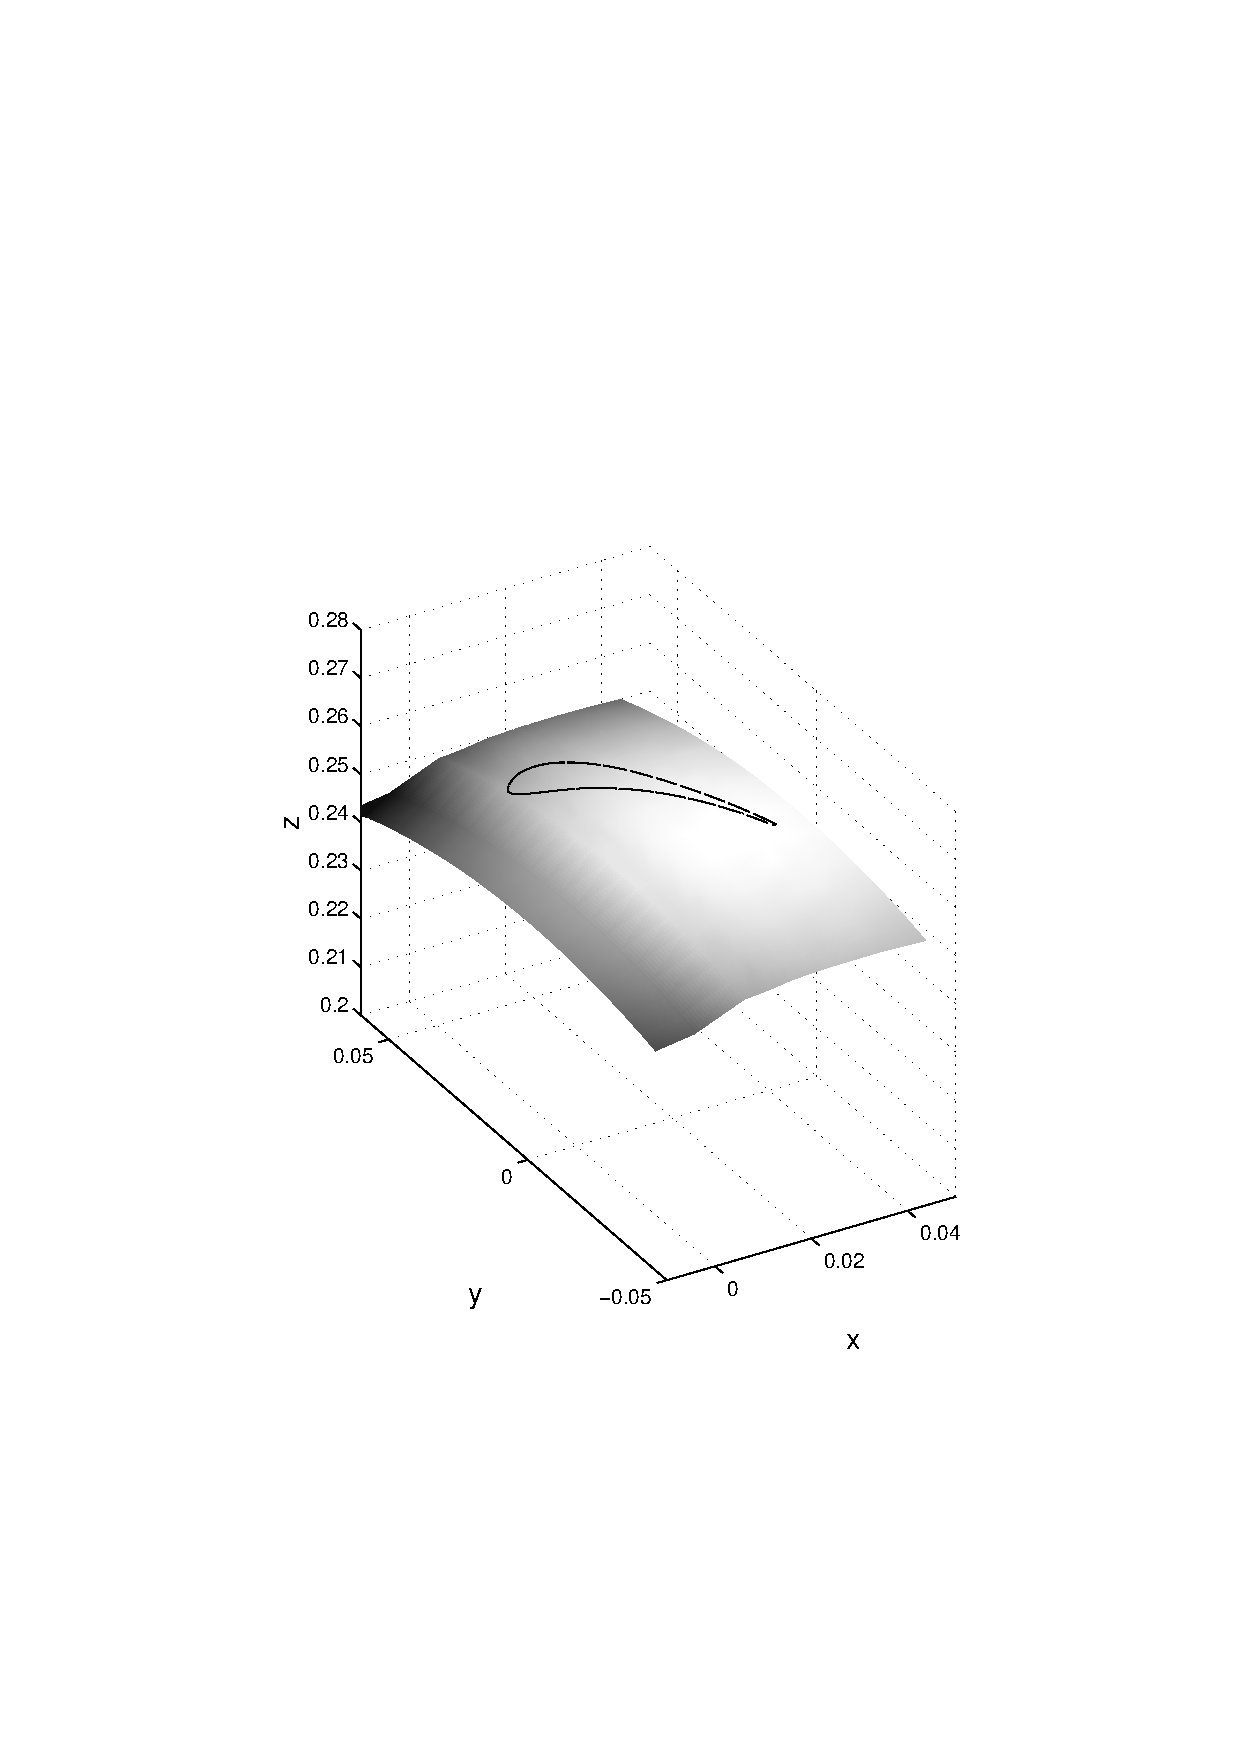
\includegraphics[width=70mm,clip=t]{CHAP_MESH/FIGURE/surf3.pdf}
      \hspace{0mm}}
    \subfigure[Tip section]
      {\hspace{0mm}
       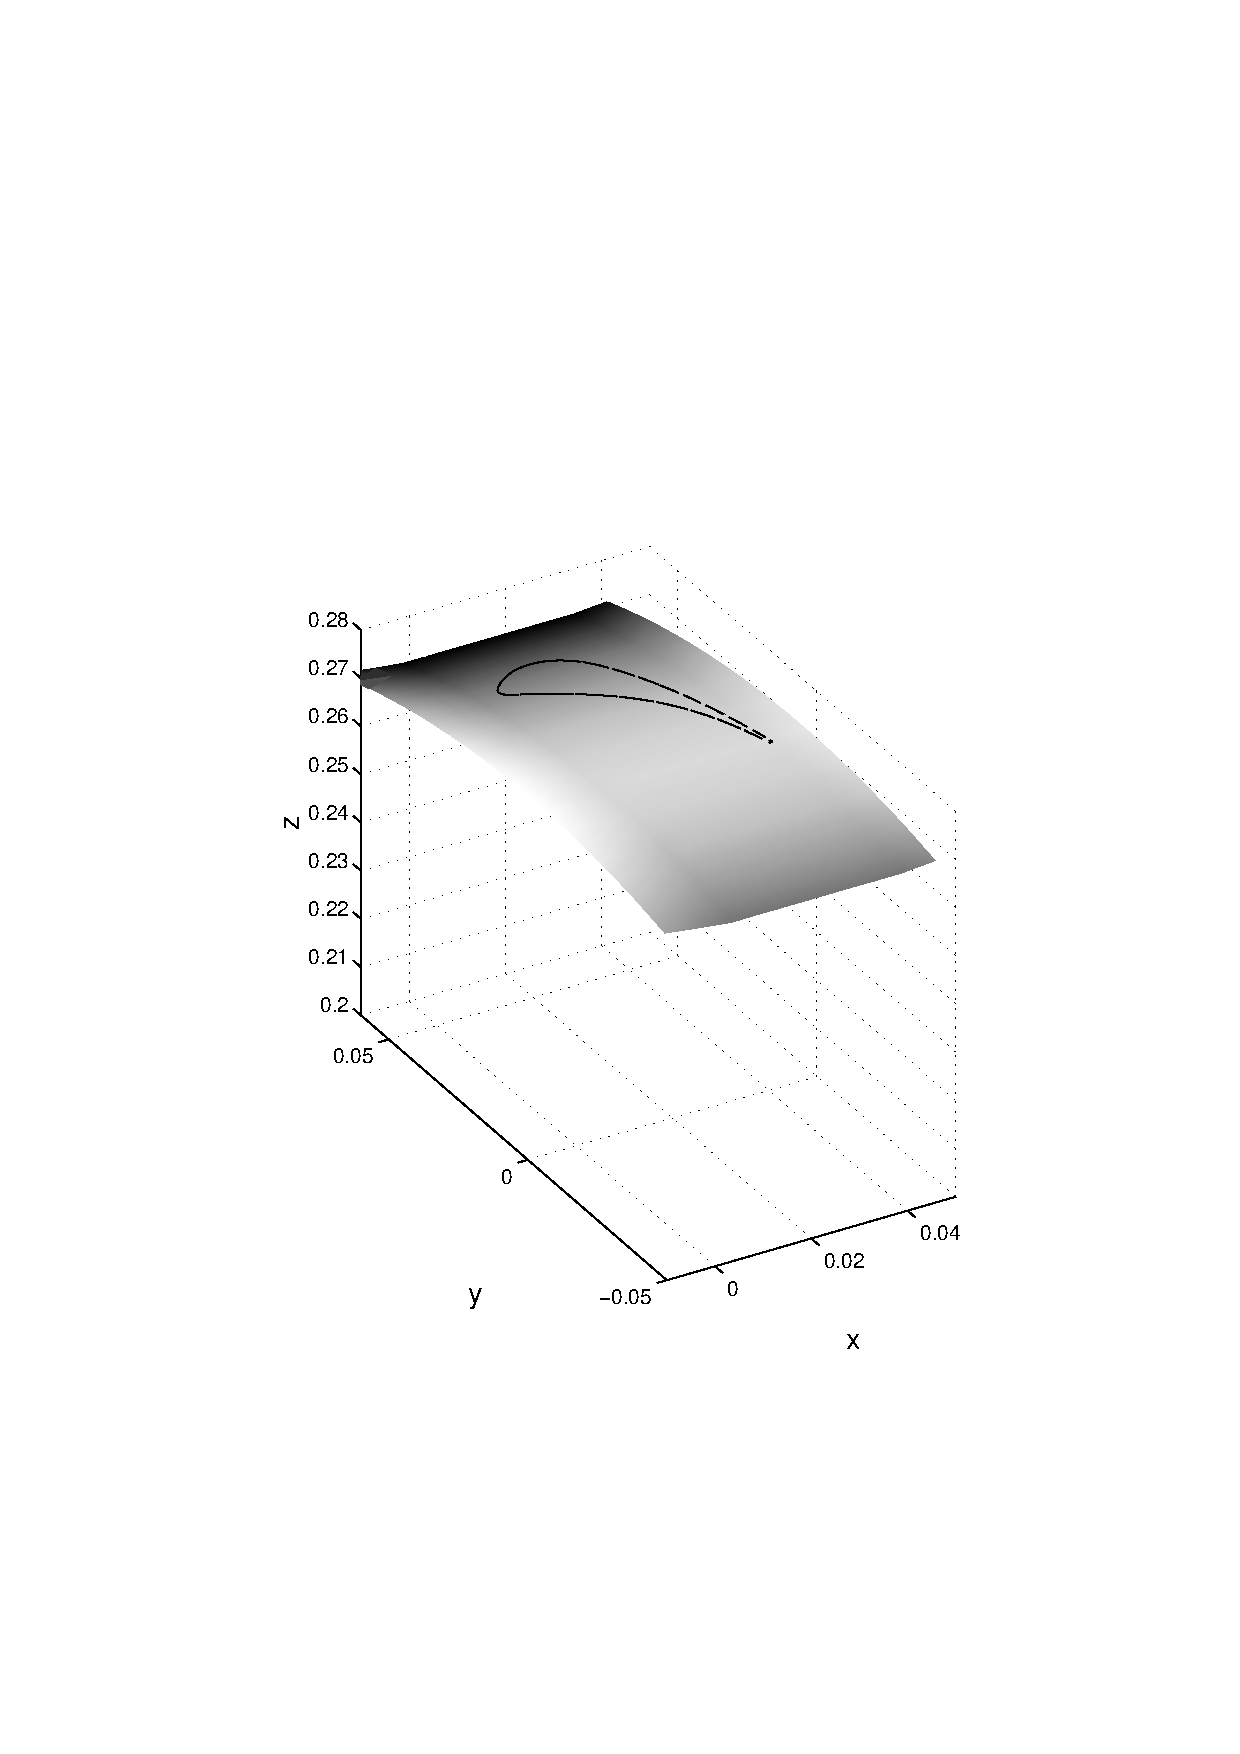
\includegraphics[width=70mm,clip=t]{CHAP_MESH/FIGURE/surf4.pdf}}
  \end{tabular}
 \end{center}
 \caption{Geometry definition of an NGV blade at different radial levels}
 \label{radial_levels.fig}
\end{figure}
%

 The starting point of the present method is the projection of
 the radial sections into parametric 2D planes,
 using the local coordinate system $u$ and $v$.
 In this way, the mesh-generation procedure will deal with
 plane sections only, thus the geometric dimension is reduced from
 three to two.
 Fig. \ref{radial_levels.fig} shows four different radial levels
 for a typical nozzle guide vane from a well-known aeroengine manufacturer.
 In this example
 $\sigma_i(x,r,\theta)$ is a surface of revolution around the $x$-axis, i.e.
 $r_{\sigma} = r\left(x\right)$.
 The parametric coordinates $u$ and $v$ are defined as:

%
\beq
  u  &=& \int\sm{x\sm{0}}\se{x} r\left(s\right) ds\\
  v  &=& r\left(x\right)\theta
\eeq
%
 Fig. \ref{radial_mapping.fig} shows the projection of the four radial
 levels shown in Fig. \ref{radial_levels.fig}.
%
\begin{figure}[ht]
 \begin{center}
  \begin{tabular}{cc}
    \subfigure[Hub section]
      {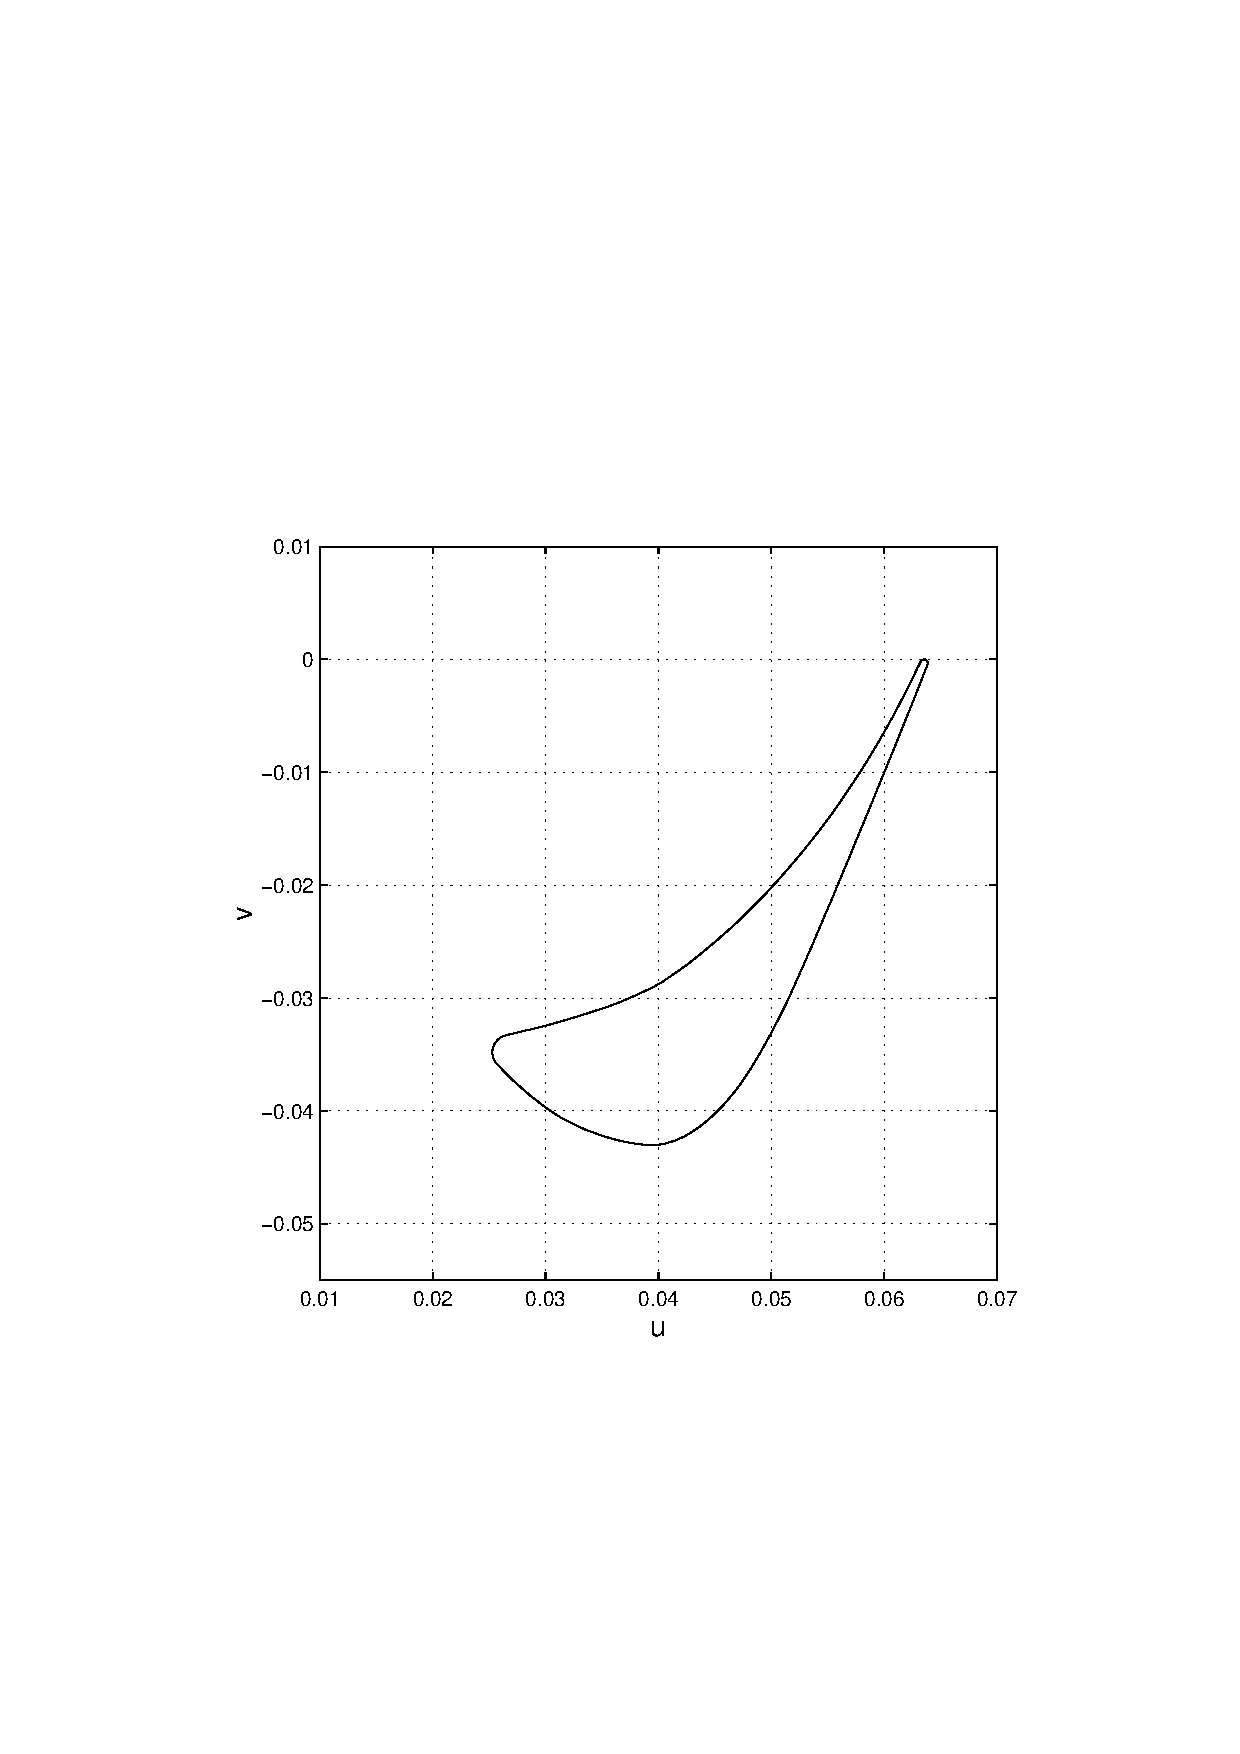
\includegraphics[width=50mm,clip=t]{CHAP_MESH/FIGURE/bla1.pdf}
      \hspace{10mm}}
    \subfigure[Hub-middle section (25\% span)]
      {\hspace{10mm}
       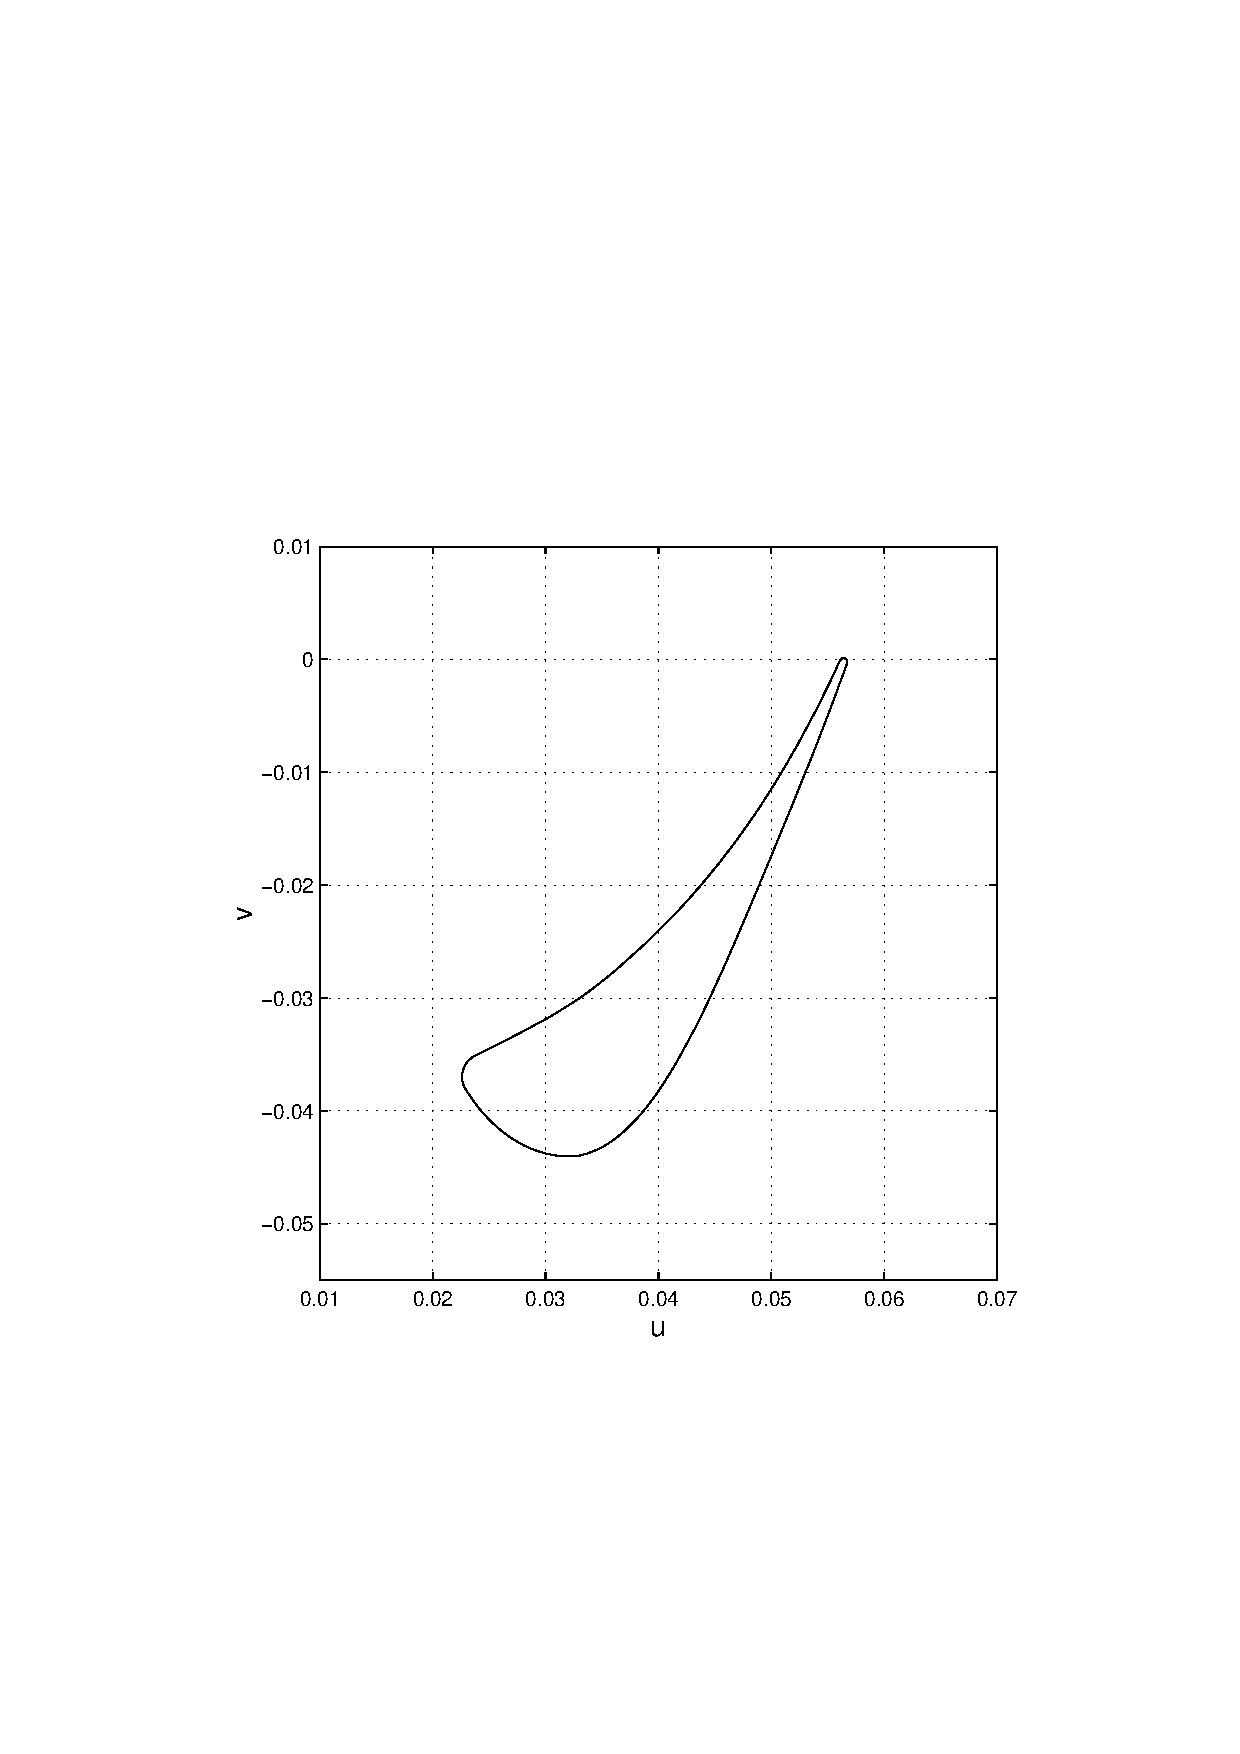
\includegraphics[width=50mm,clip=t]{CHAP_MESH/FIGURE/bla2.pdf}}
    \\
    \subfigure[Tip-middle section (75\% span)]
      {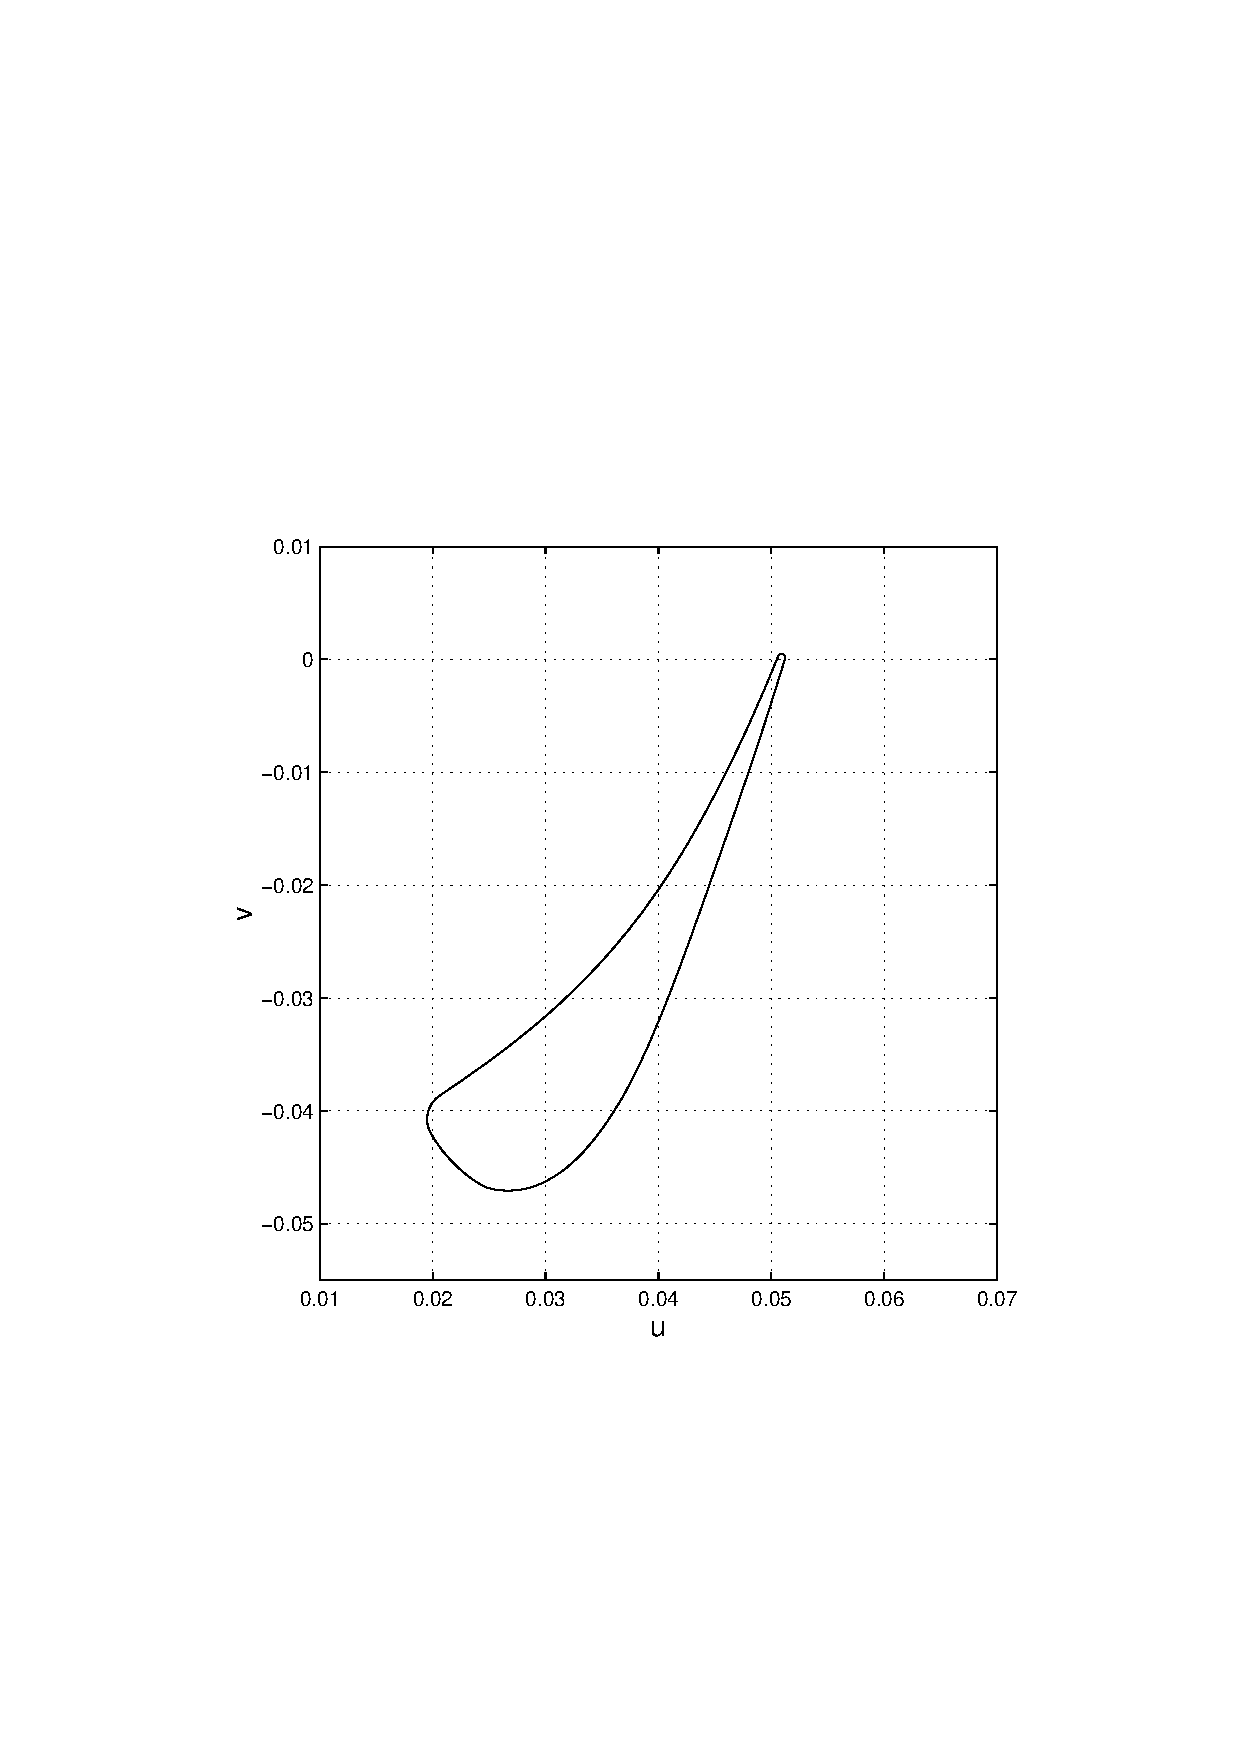
\includegraphics[width=50mm,clip=t]{CHAP_MESH/FIGURE/bla3.pdf}
      \hspace{10mm}}
    \subfigure[Tip section]
      {\hspace{10mm}
       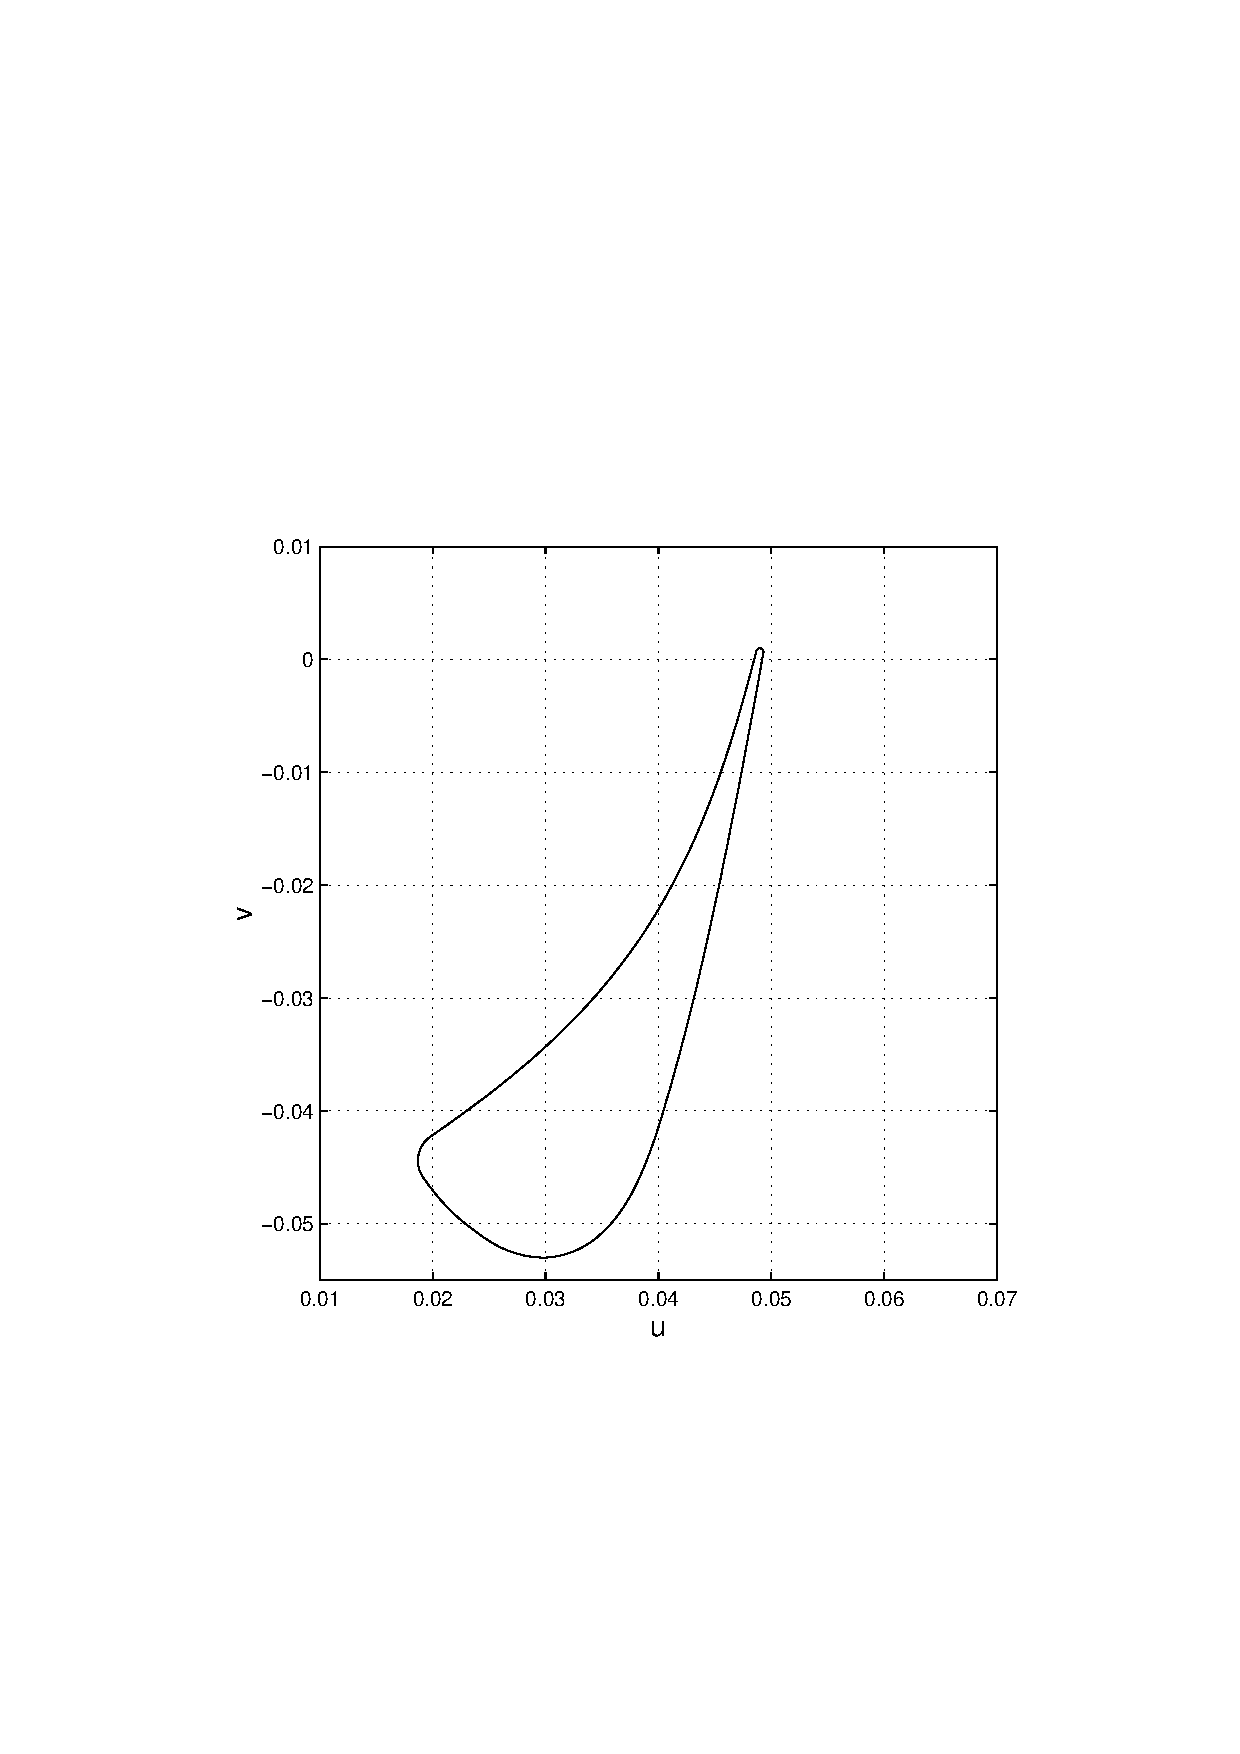
\includegraphics[width=50mm,clip=t]{CHAP_MESH/FIGURE/bla4.pdf}}
  \end{tabular}
 \end{center}
 \vspace{-5mm}
 \caption{Parametric 2D planes for four different radial levels}
 \label{radial_mapping.fig}
\end{figure}
%
%
\subsection{Unstructured mesh generation}
%
 Once all radial sections are projected into 2D planes,
 a hybrid quadrilateral-triangular mesh is generated in the 2D master plane
 which corresponds to a certain radial level (usually the middle one).
 The quadrilateral part of the mesh takes the form of a body-fitted
 O-grid which is generated using an advancing normal method.
 The orthogonality of this structured mesh is very important for
 an accurate resolution of the turbulent-boundary layer which
 originates from high Reynolds number flows. This point will be
 stressed further in the next chapter where a novel finite-volume discretisation
 of the Navier-Stokes equations on hybrid grids will be explored.
 The remaining part of the domain is discretised using an unstructured
 mesh generator which uses an advancing front algorithm (Morgan et al.
 \citeyearNP{Peiro:1}, Mavriplis \citeyearNP{Mavriplis:2}).
 A distinctive feature of this method is that both triangles and
 points are generated simultaneously.
 Such an approach enables the generation of elements
 with variable sizes and stretching, and hence it differs from Delaunay-type
 mesh generators (Baker \citeyearNP{Delaunay},
 Mavriplis \citeyearNP{Mavriplis:2}).

 Fig. \ref{mesh2d_master.fig}b shows the final unstructured hybrid-grid
 of the NGV in Fig. \ref{radial_levels.fig}
 in the 2D master plane which, in this case, corresponds to the projected
 middle section of the 3D blade.

%
%
\subsection{Quasi-conformal mapping}
%
 An important part of the mesh-generation strategy is
 the mapping procedure to project the 2D unstructured mesh of
 the master plane back to all radial blade-definition levels.
 A necessary condition for a mapping function is that
 it must associate a given point of the master plane with one,
 and only one, point of the target plane.
 Moreover a mapping function should also guarantee
 that a given angle in the master plane is mapped into a similar-valued angle
 in the target plane (quasi-conformal mapping). This last property is essential
 in order to minimize the skewness of the mesh, especially for
 highly-twisted blades.

 The starting point for the quasi-conformal mapping is the generation
 of coarse structured quadrilateral grids for all projected radial levels,
 including the master plane.
 Following the approach of Steger \& Sorenson \citeyear{Ellipt2},
 these meshes are obtained by solving a system of elliptic partial-differential
 equations.
 An essential requirement for such structured meshes is that they must
 be generated in exactly the same manner, i.e. with the same number of
 points and quadrilaterals for all radial levels.
 Fig. \ref{mesh2d_master.fig} shows the structured quadrilateral grid
 and the unstructured hybrid-grid in the master plane, which correspond
 to the middle radial section.
%
\begin{figure}[ht]
 \begin{center}
  \begin{tabular}{cc}
    \subfigure[Structured mesh for mapping]
      {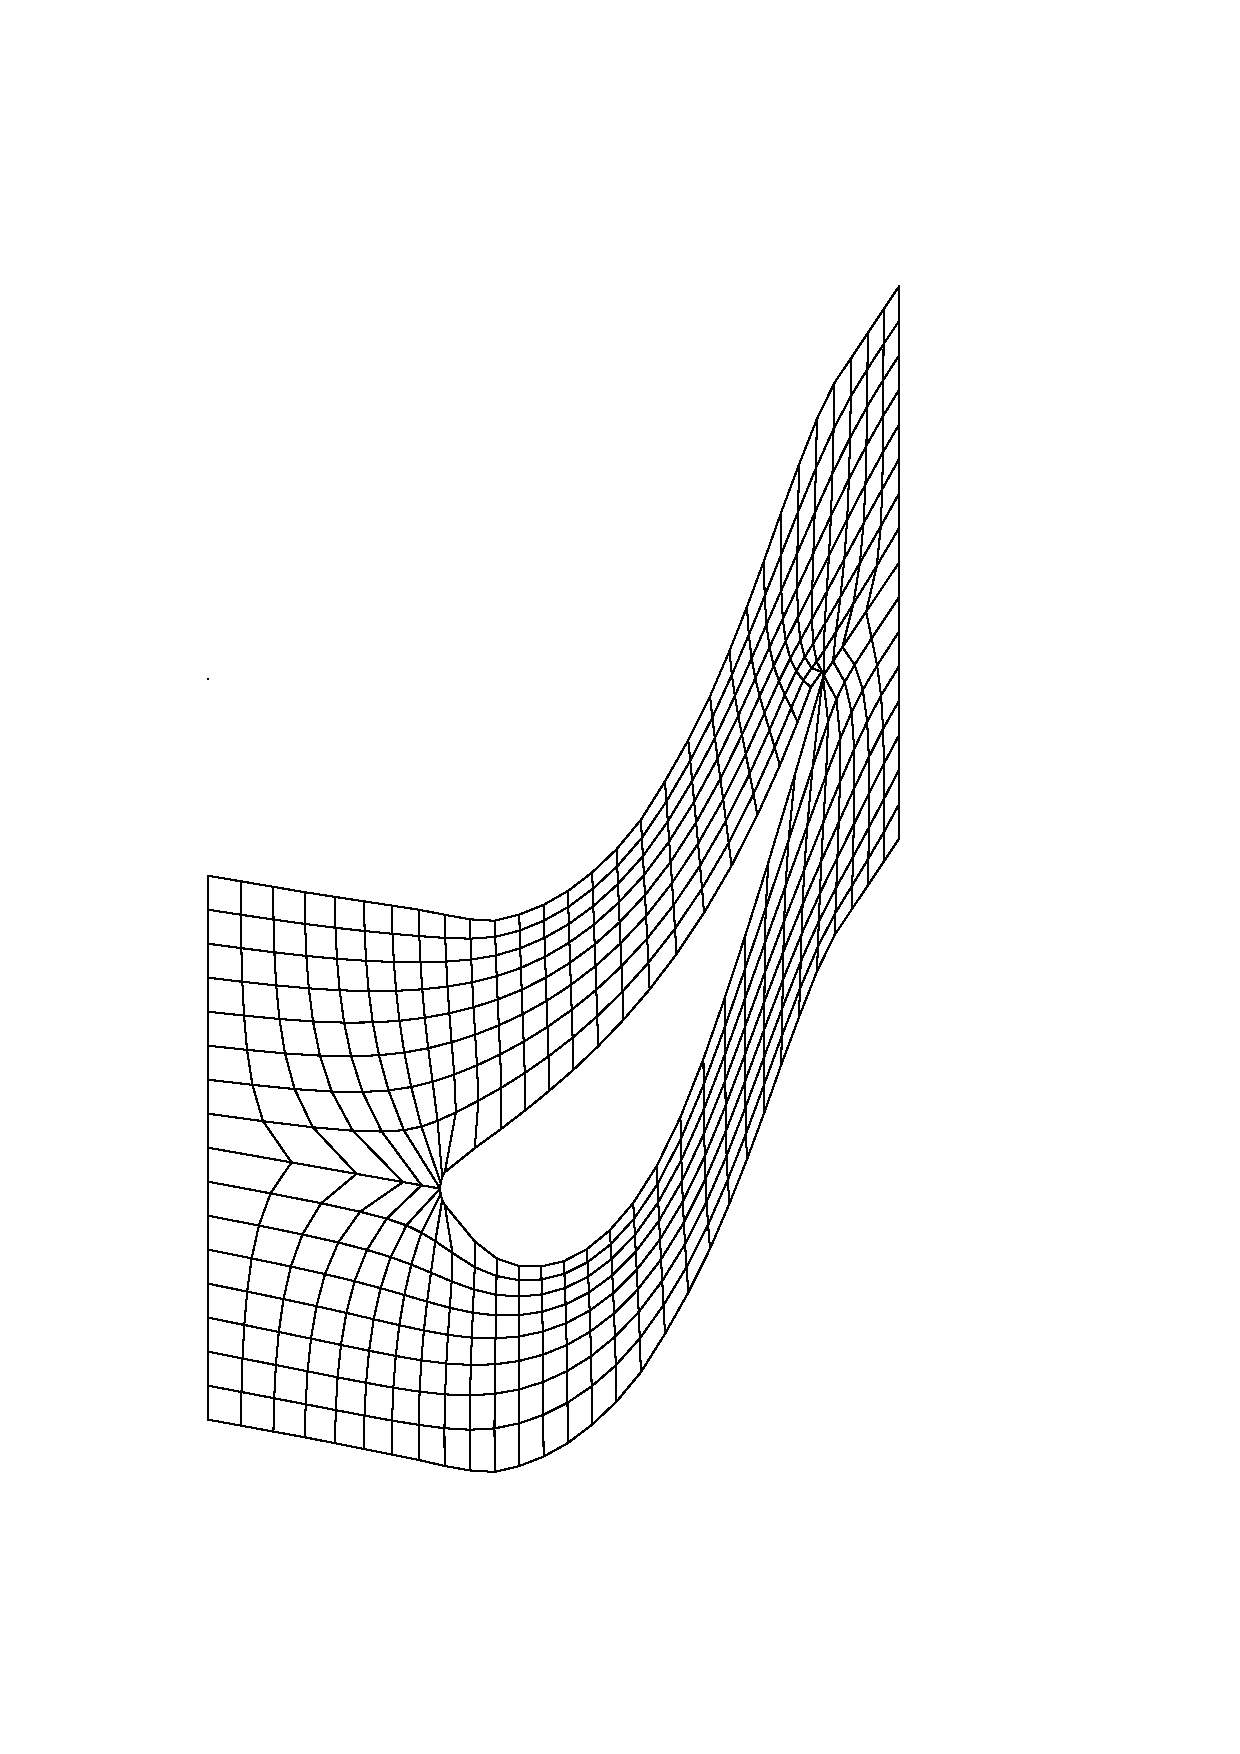
\includegraphics[width=70mm,clip=t]{CHAP_MESH/FIGURE/mesh2d_struct.pdf}}
    \subfigure[Unstructured mesh]
      {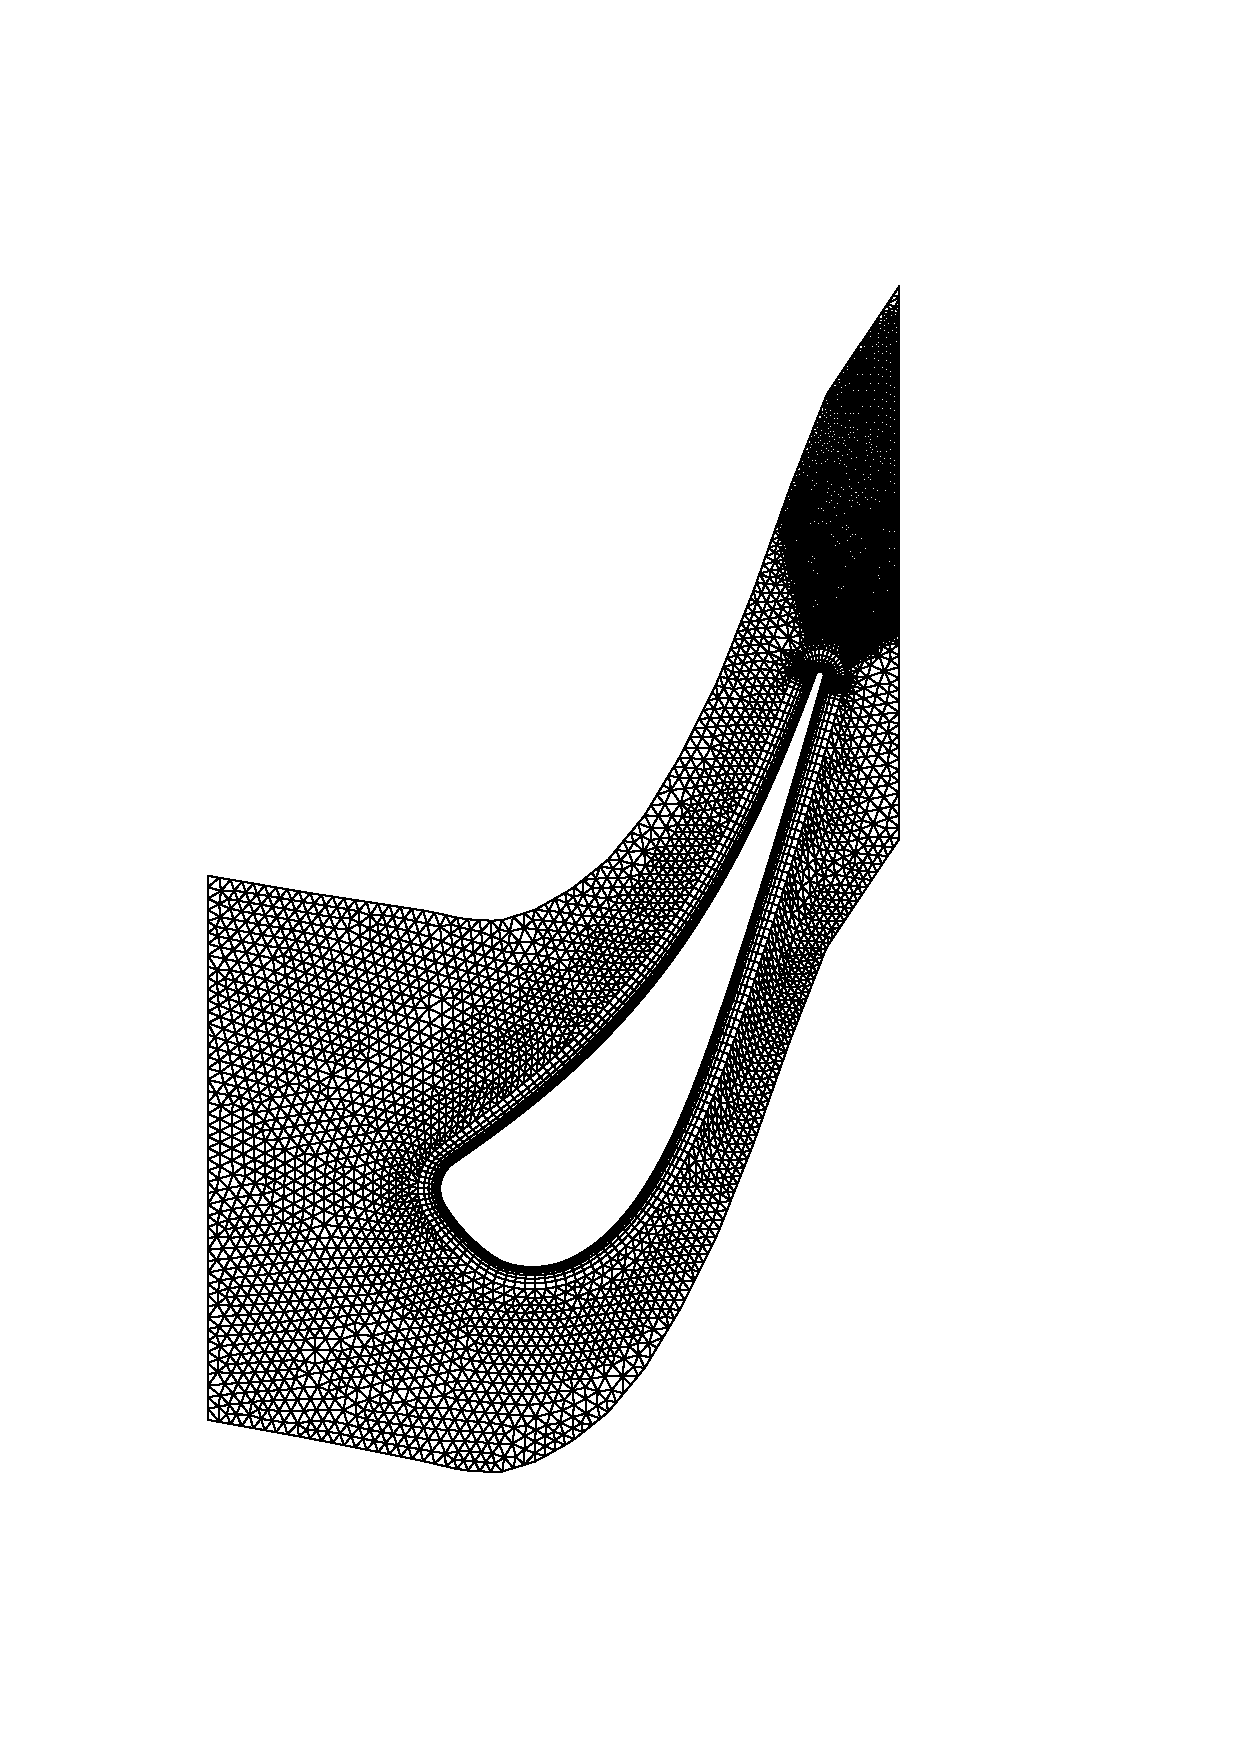
\includegraphics[width=70mm,clip=t]{CHAP_MESH/FIGURE/mesh2d_unstruct.pdf}}
  \end{tabular}
 \end{center}
 \vspace{-5mm}
 \caption{Meshes in the master plane}
 \label{mesh2d_master.fig}
\end{figure}
%
 The mapping procedure is divided into three different steps.
%
\paragraph{\bf Geometry searching in the master plane.}
 Each point $J$ of the unstructured 2D mesh in Fig \ref{mesh2d_master.fig}b
 must be located on quadrilateral $E$ of the structured mesh in
 Fig \ref{mesh2d_master.fig}a.
%
 \paragraph{\bf Inverse mapping in the master plane.}
 The Cartesian coordinates
 $\vec{x}\sm{J} = \left(x\sm{J}, y\sm{J}\right)$ of point $J$,
 associated with the quadrilateral $E$ are given by
%
\begin{equation}
  \vec{x}\sm{J} = \sum_{I=1}^4 \vec{x}\sm{I}
                   N\sm{I} \left(\xi\sm{J},\eta\sm{J}\right)
  \label{mapping_1}
\end{equation}
%
 where $\left(\xi\sm{J},\eta\sm{J}\right)$ represent the local-coordinates,
 $\vec{x}\sm{I}$ represents the Cartesian coordinates of nodes $I=1,\dots,4$
 of the quadrilateral $E$ and
 $N\sm{I}$ is the standard finite-element bilinear shape-function
 which takes the form (Zienkiewicz \& Morgan \citeyearNP{Zienk:1}):
%
\begin{equation}
  N\sm{I} = \frac{1}{4} \left\{
  \begin{array}{l}
     \left(1 - \xi\right) \left(1 - \eta\right) \\
     \left(1 + \xi\right) \left(1 - \eta\right) \\
     \left(1 + \xi\right) \left(1 + \eta\right) \\
     \left(1 - \xi\right) \left(1 + \eta\right)
  \end{array}
  \right.
  \label{shape_function}
\end{equation}
%
 A Newton-Raphson method is used in order to obtain the values of
 $\xi\sm{J}$ and $\eta\sm{J}$.
%
 \paragraph{\bf Direct mapping.}
 Once all points $J$ of the
 unstructured mesh in the master plane are associated with quadrilateral
 $E$ and local-coordinates $\left(\xi\sm{J},\eta\sm{J}\right)$
 are determined, coordinates $\vec{x}\sm{J}$ of points
 on the remaining projected radial sections are obtained
 directly using equation (\ref{mapping_1}).
\vspace{5mm}

 The above-described steps are shown in Fig. \ref{mapping.fig}.
%
\begin{figure}[ht]
   \centerline{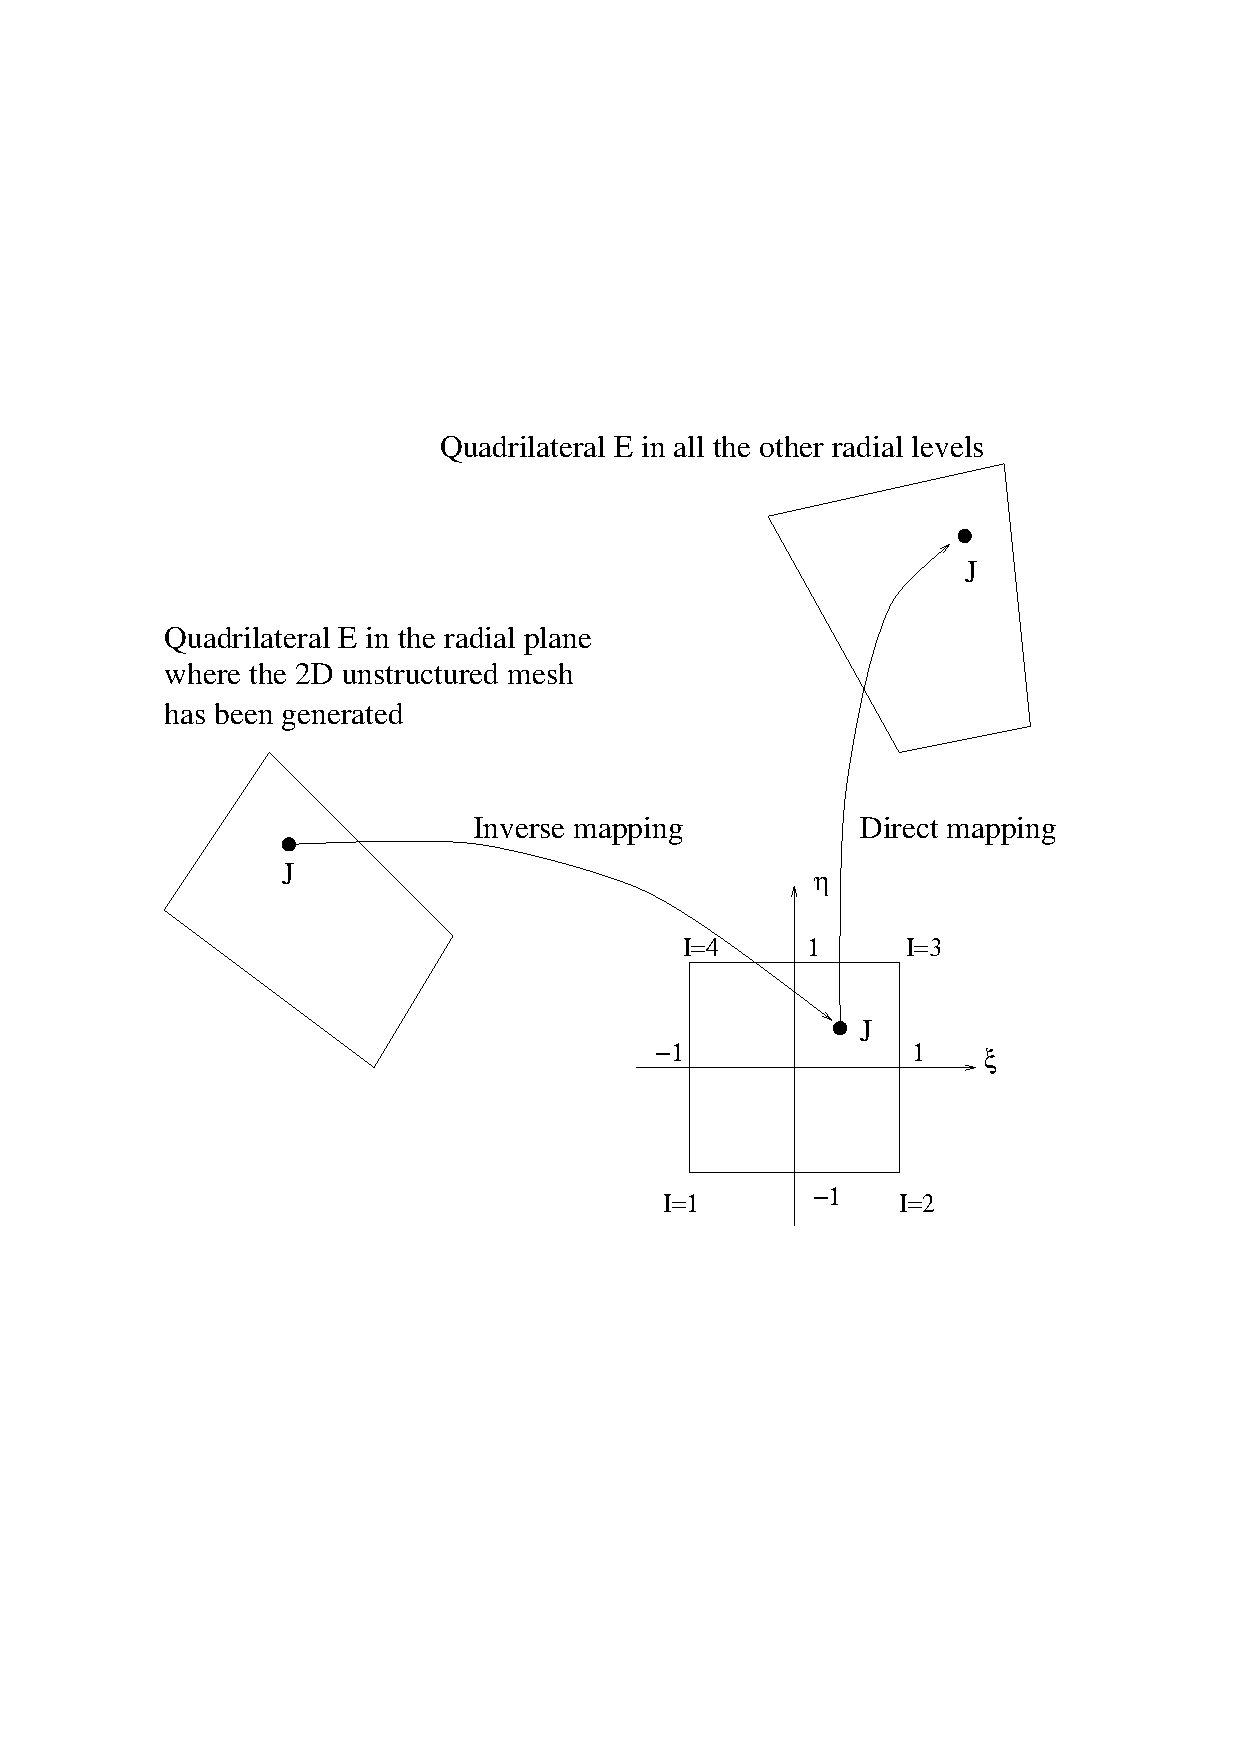
\includegraphics[width=120mm,clip=t]{CHAP_MESH/FIGURE/mapping.pdf}}
   \caption{Mapping procedure}
   \label{mapping.fig}
\end{figure}
%
 The mapping method becomes fully conformal if (i) a given element of the 2D
 hybrid mesh lies within a single quadrilateral of the structured
 grid. (ii) In addition, the angles of this quadrilateral must remain the
 same for all radial sections.
 If the above two conditions are not
 satisfied, the conformal property is not guaranteed and, for this reason,
 the procedure has been labelled quasi-conformal here.
 Finally, it is worth noting that the algorithm is not CPU-intensive,
 since the geometry searching and
 the inverse-mapping are performed once only.

 Fig. \ref{mesh2d_other.fig} shows the structured meshes used for mapping
 and the corresponding mapped unstructured hybrid-grids at three radial levels.
%
\begin{figure}
 \begin{center}
  \begin{tabular}{c}
    \subfigure[Hub section]
      {\begin{tabular}{cc}
      {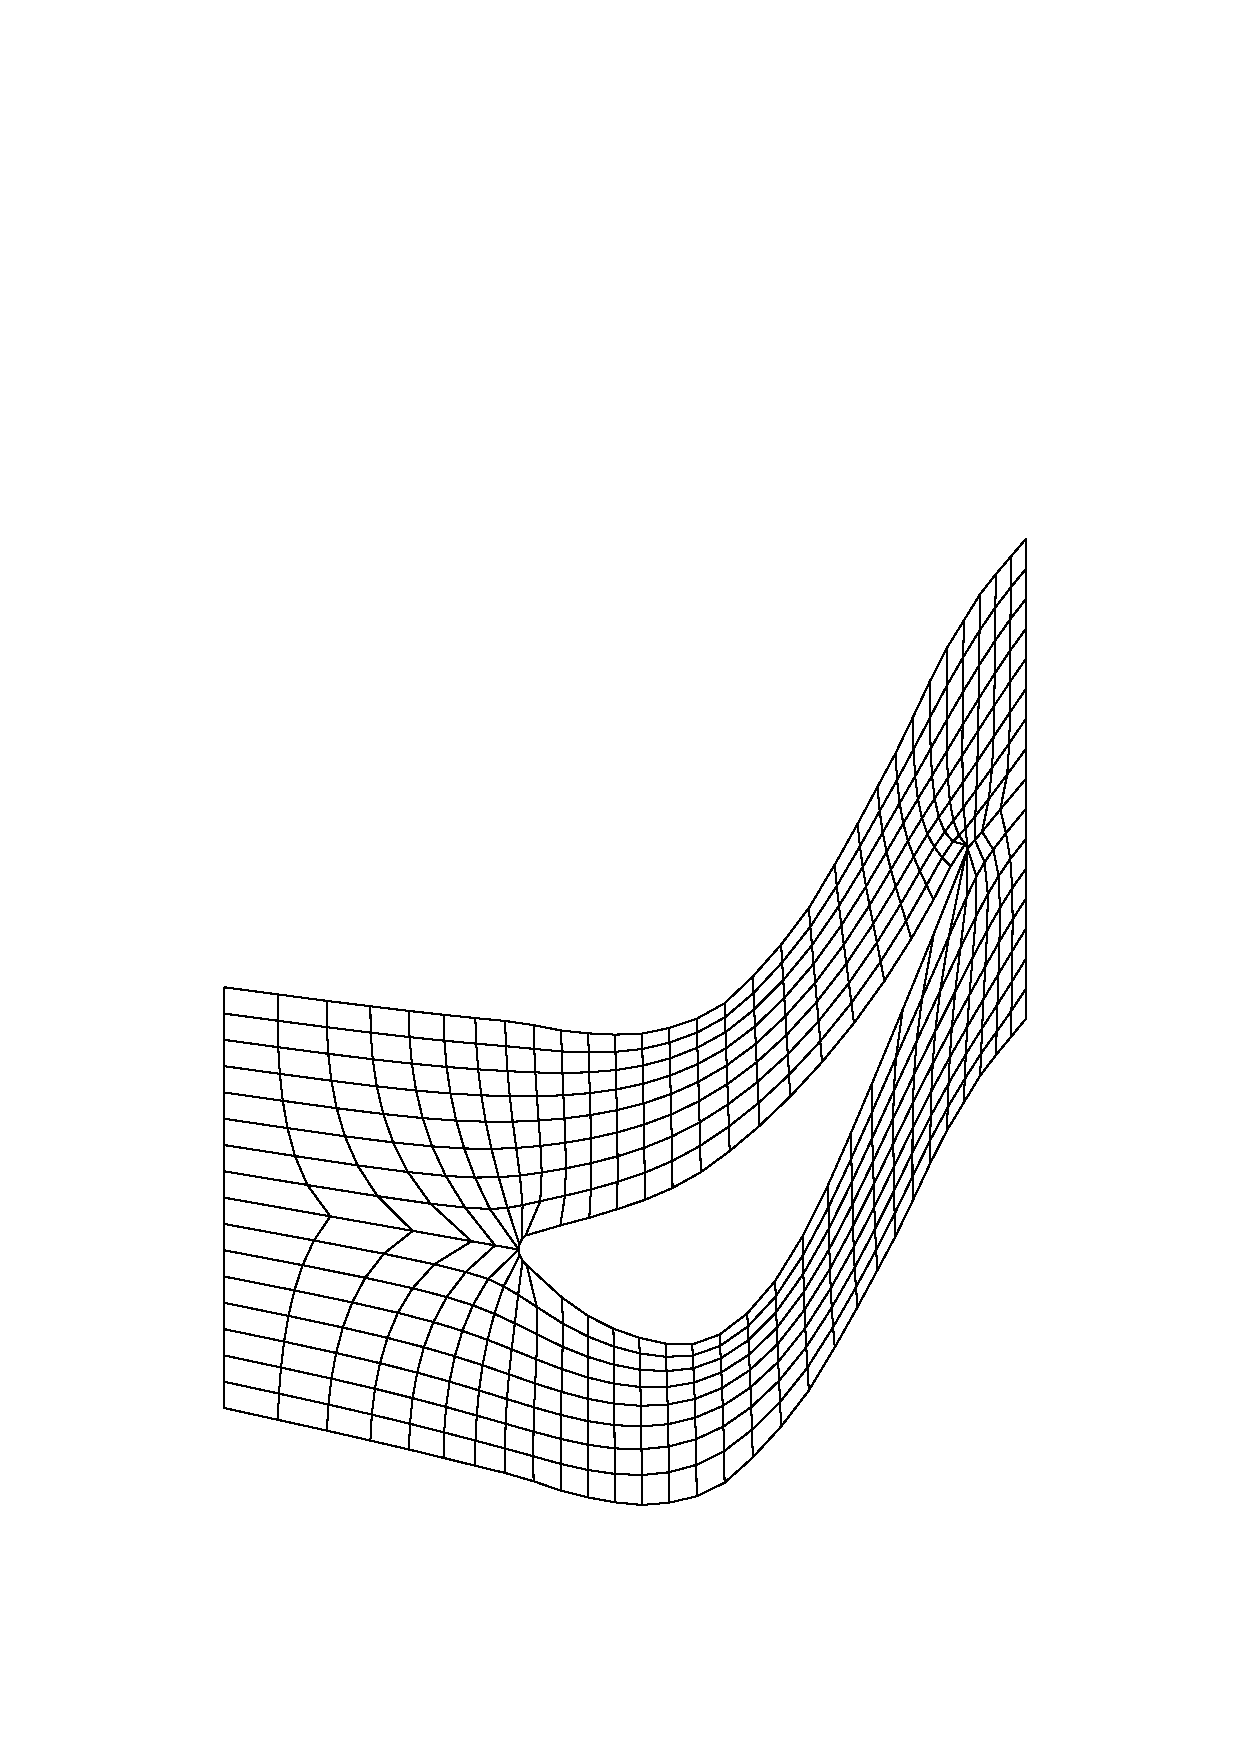
\includegraphics[width=45mm,clip=t]{CHAP_MESH/FIGURE/mesh2d_1_struct.pdf}\hspace{10mm}}
      &
      {\hspace{10mm}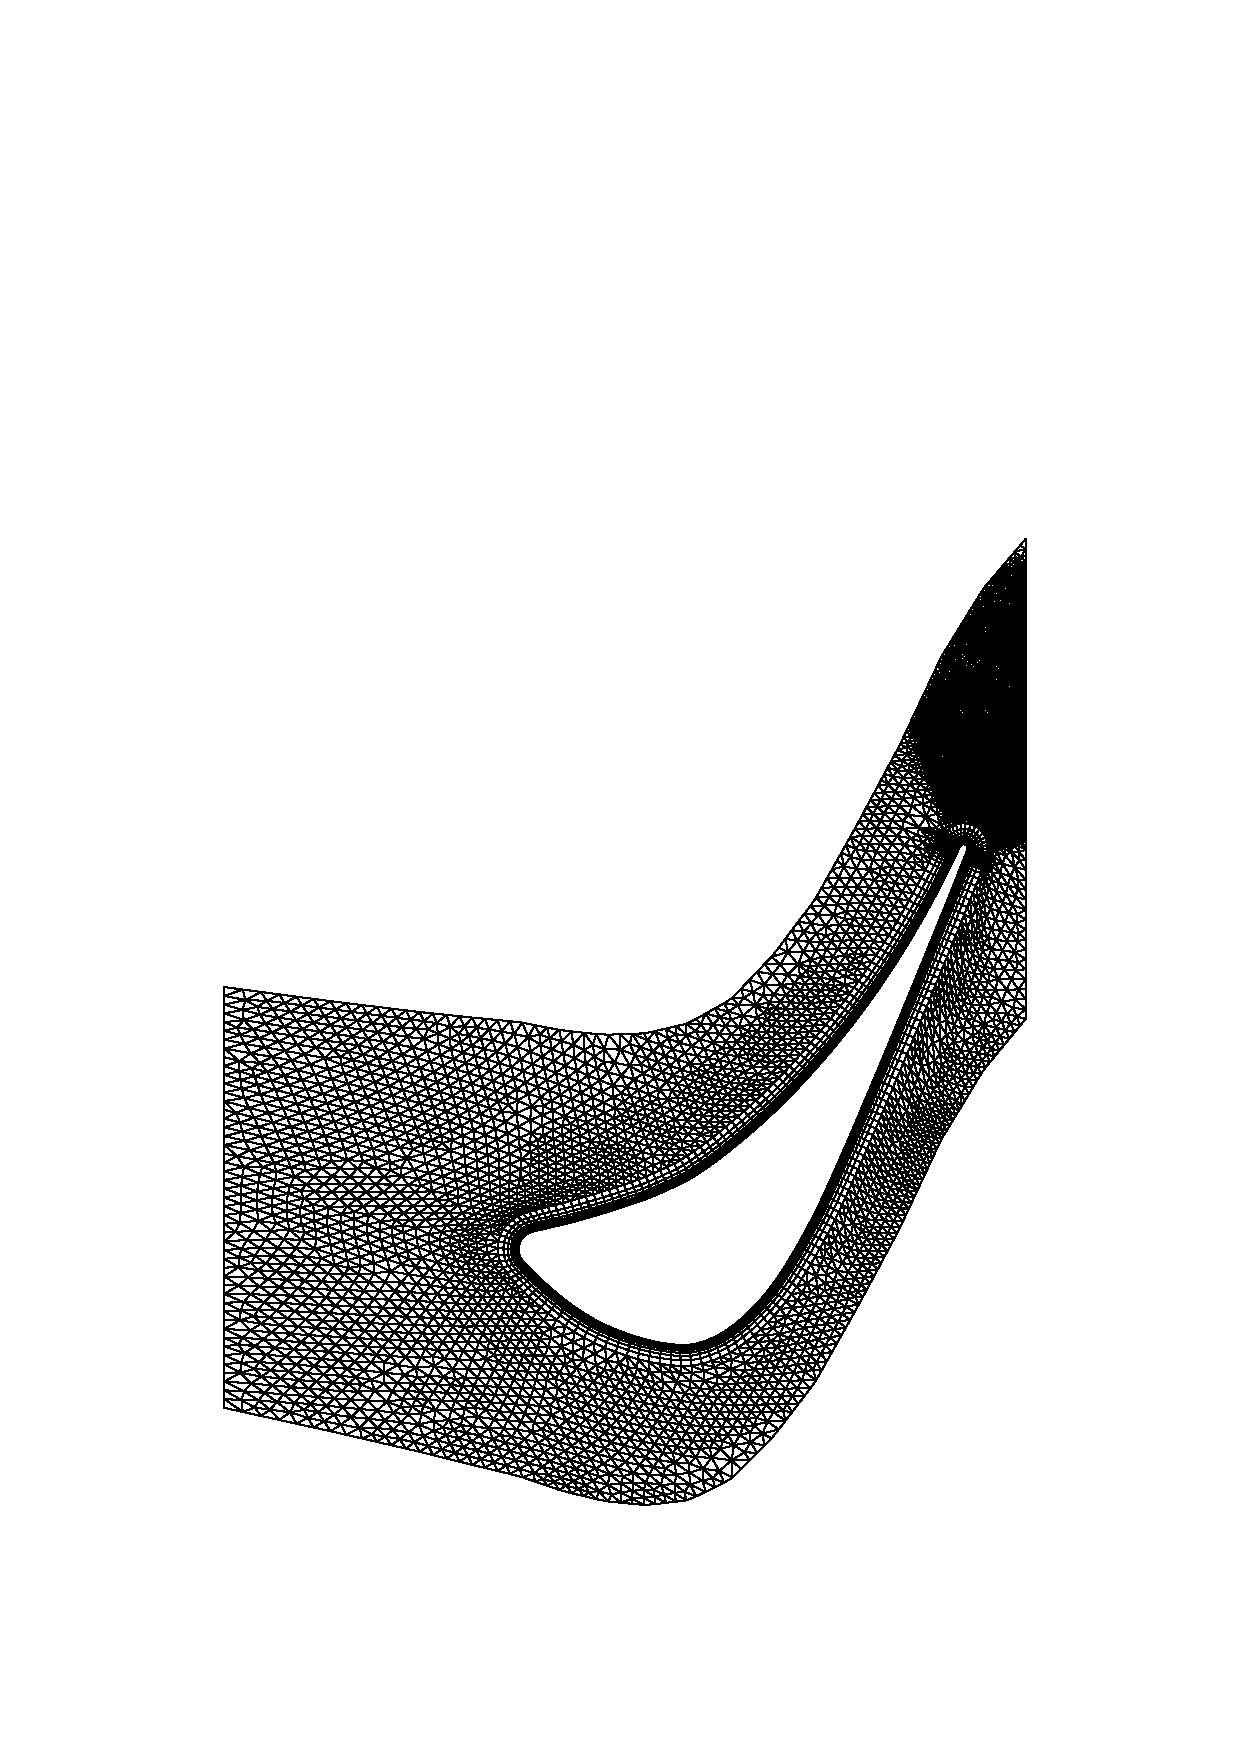
\includegraphics[width=45mm,clip=t]{CHAP_MESH/FIGURE/mesh2d_1_unstruct.pdf}}
      \end{tabular}}
    \\
    \subfigure[Middle section]
      {\begin{tabular}{cc}
      {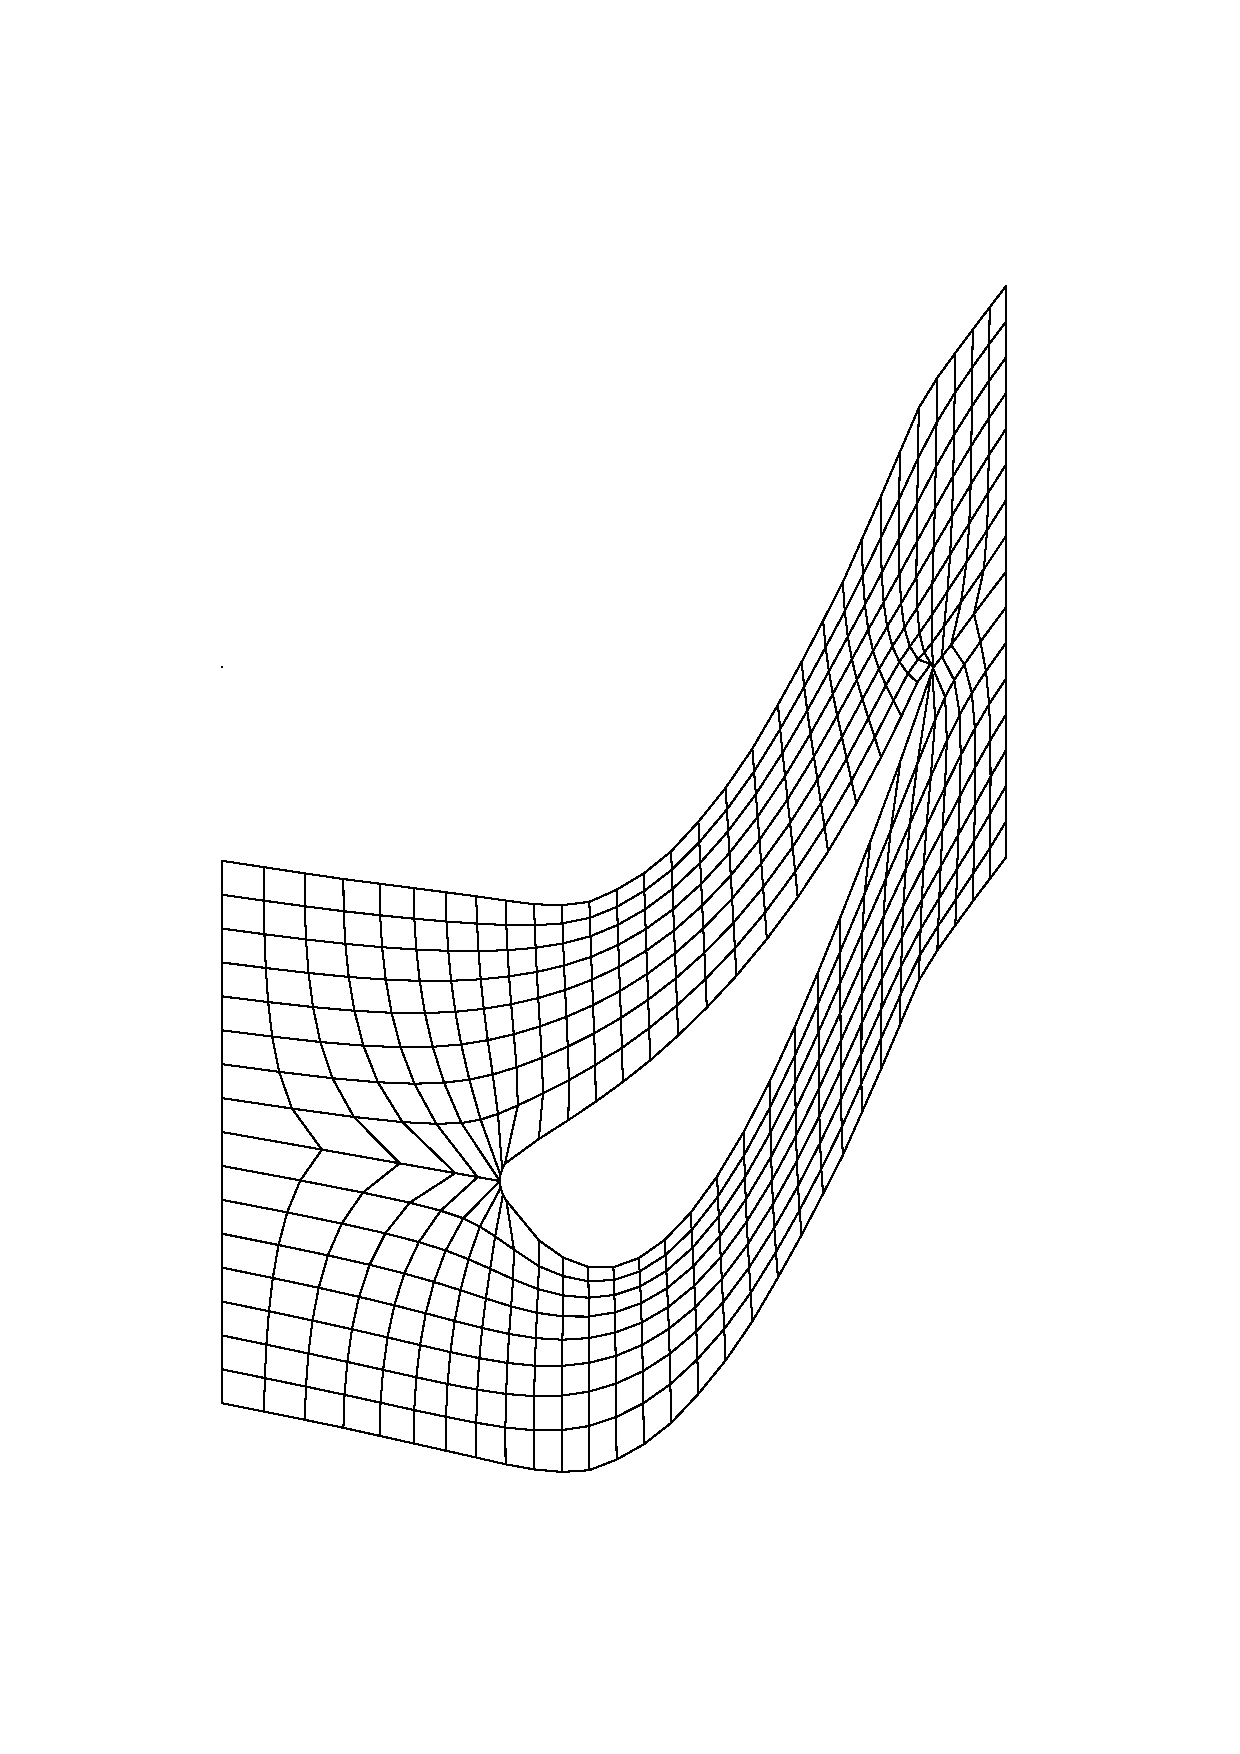
\includegraphics[width=45mm,clip=t]{CHAP_MESH/FIGURE/mesh2d_2_struct.pdf}\hspace{10mm}}
      &
      {\hspace{10mm}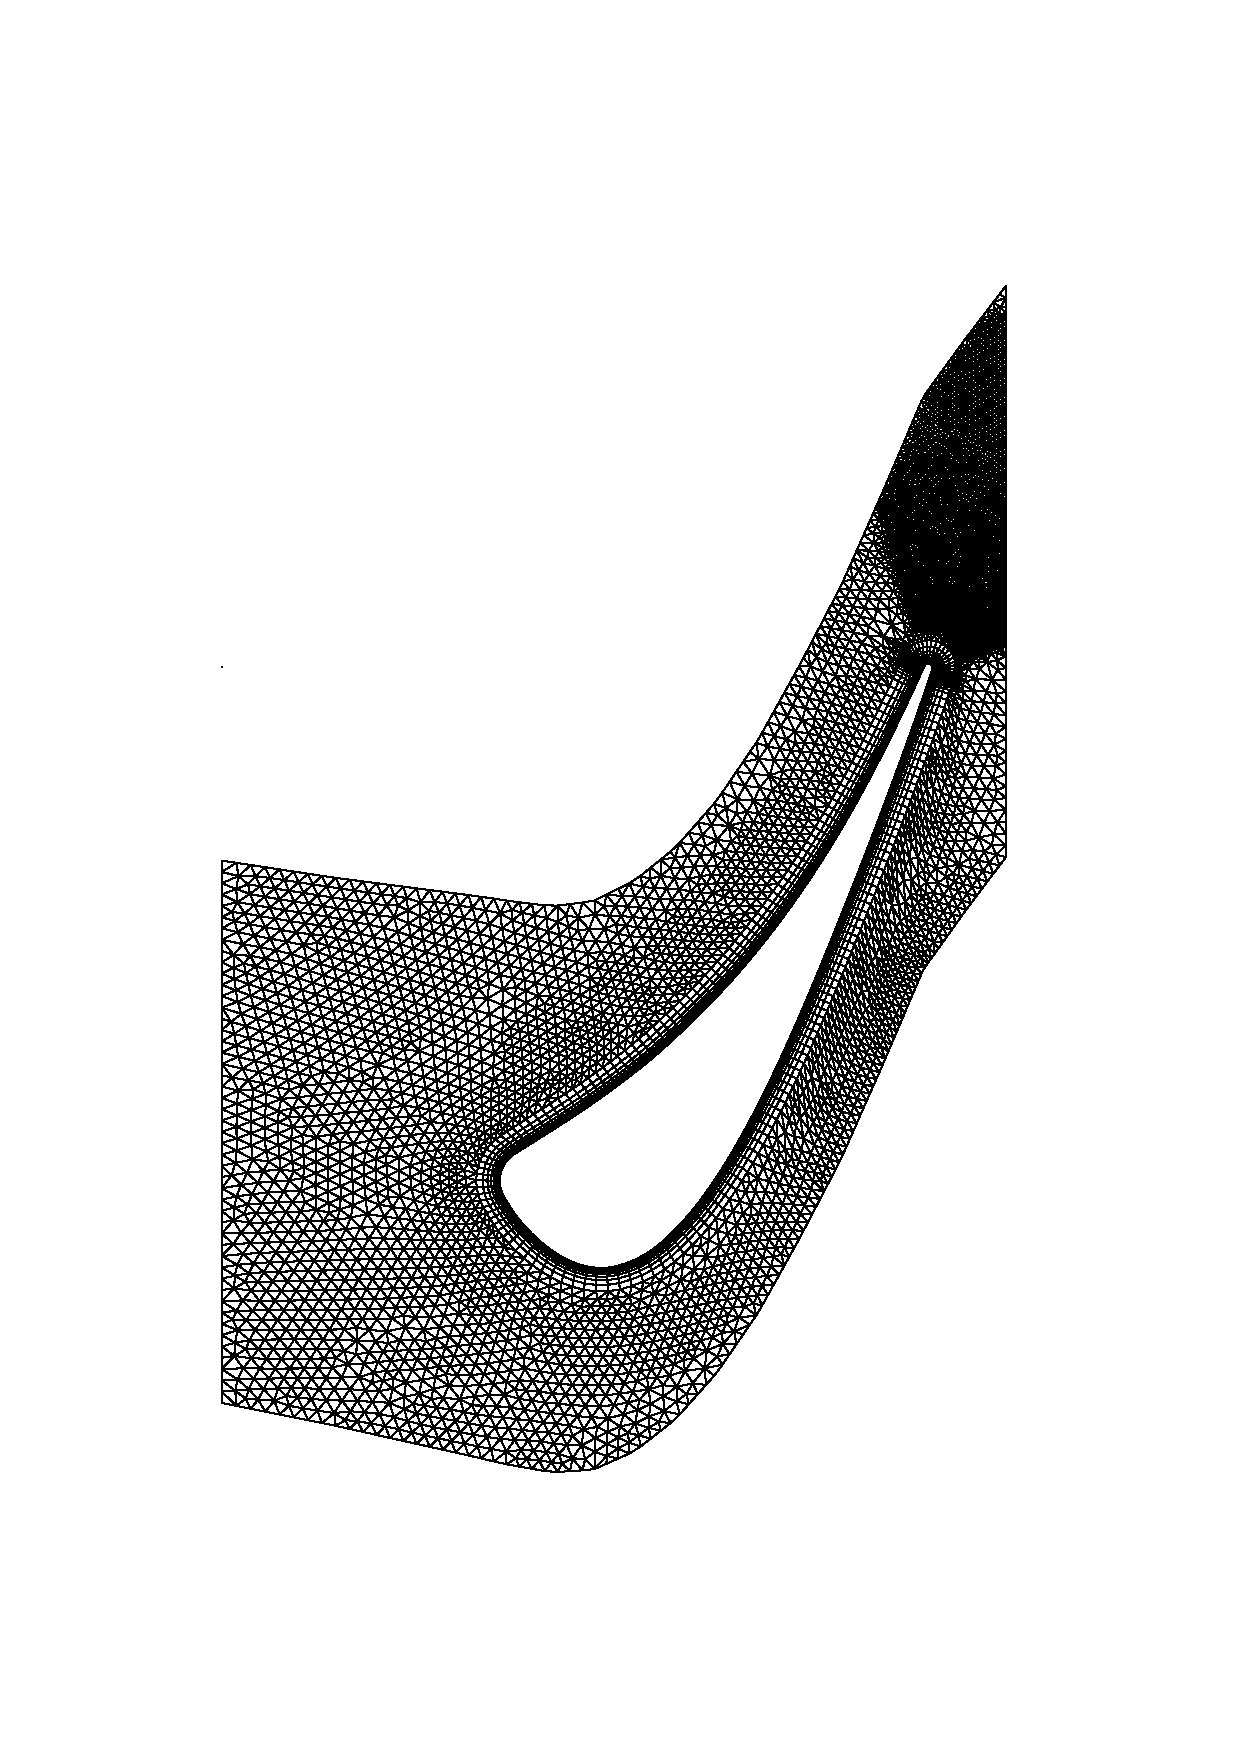
\includegraphics[width=45mm,clip=t]{CHAP_MESH/FIGURE/mesh2d_2_unstruct.pdf}}
      \end{tabular}}
    \\
    \subfigure[Tip section]
      {\begin{tabular}{cc}
      {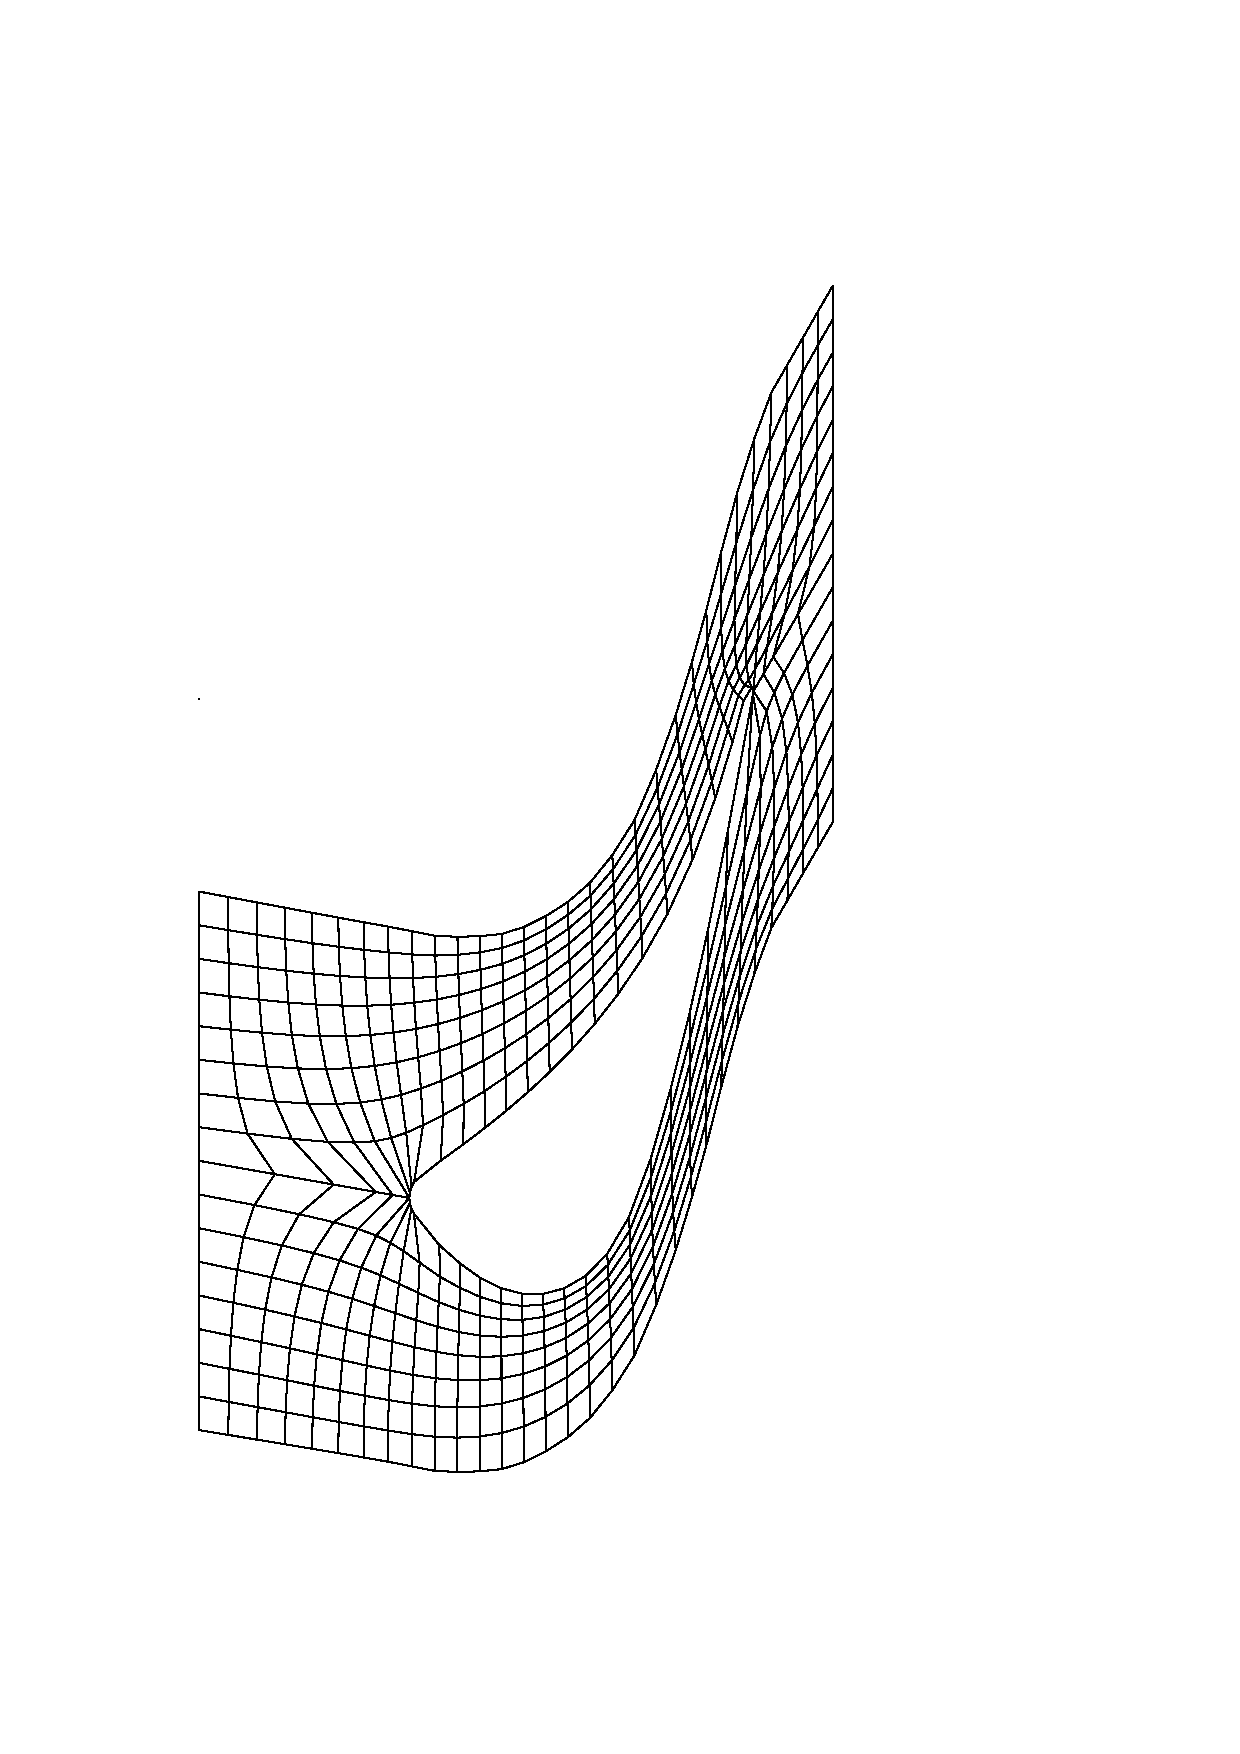
\includegraphics[width=45mm,clip=t]{CHAP_MESH/FIGURE/mesh2d_3_struct.pdf}\hspace{10mm}}
      &
      {\hspace{10mm}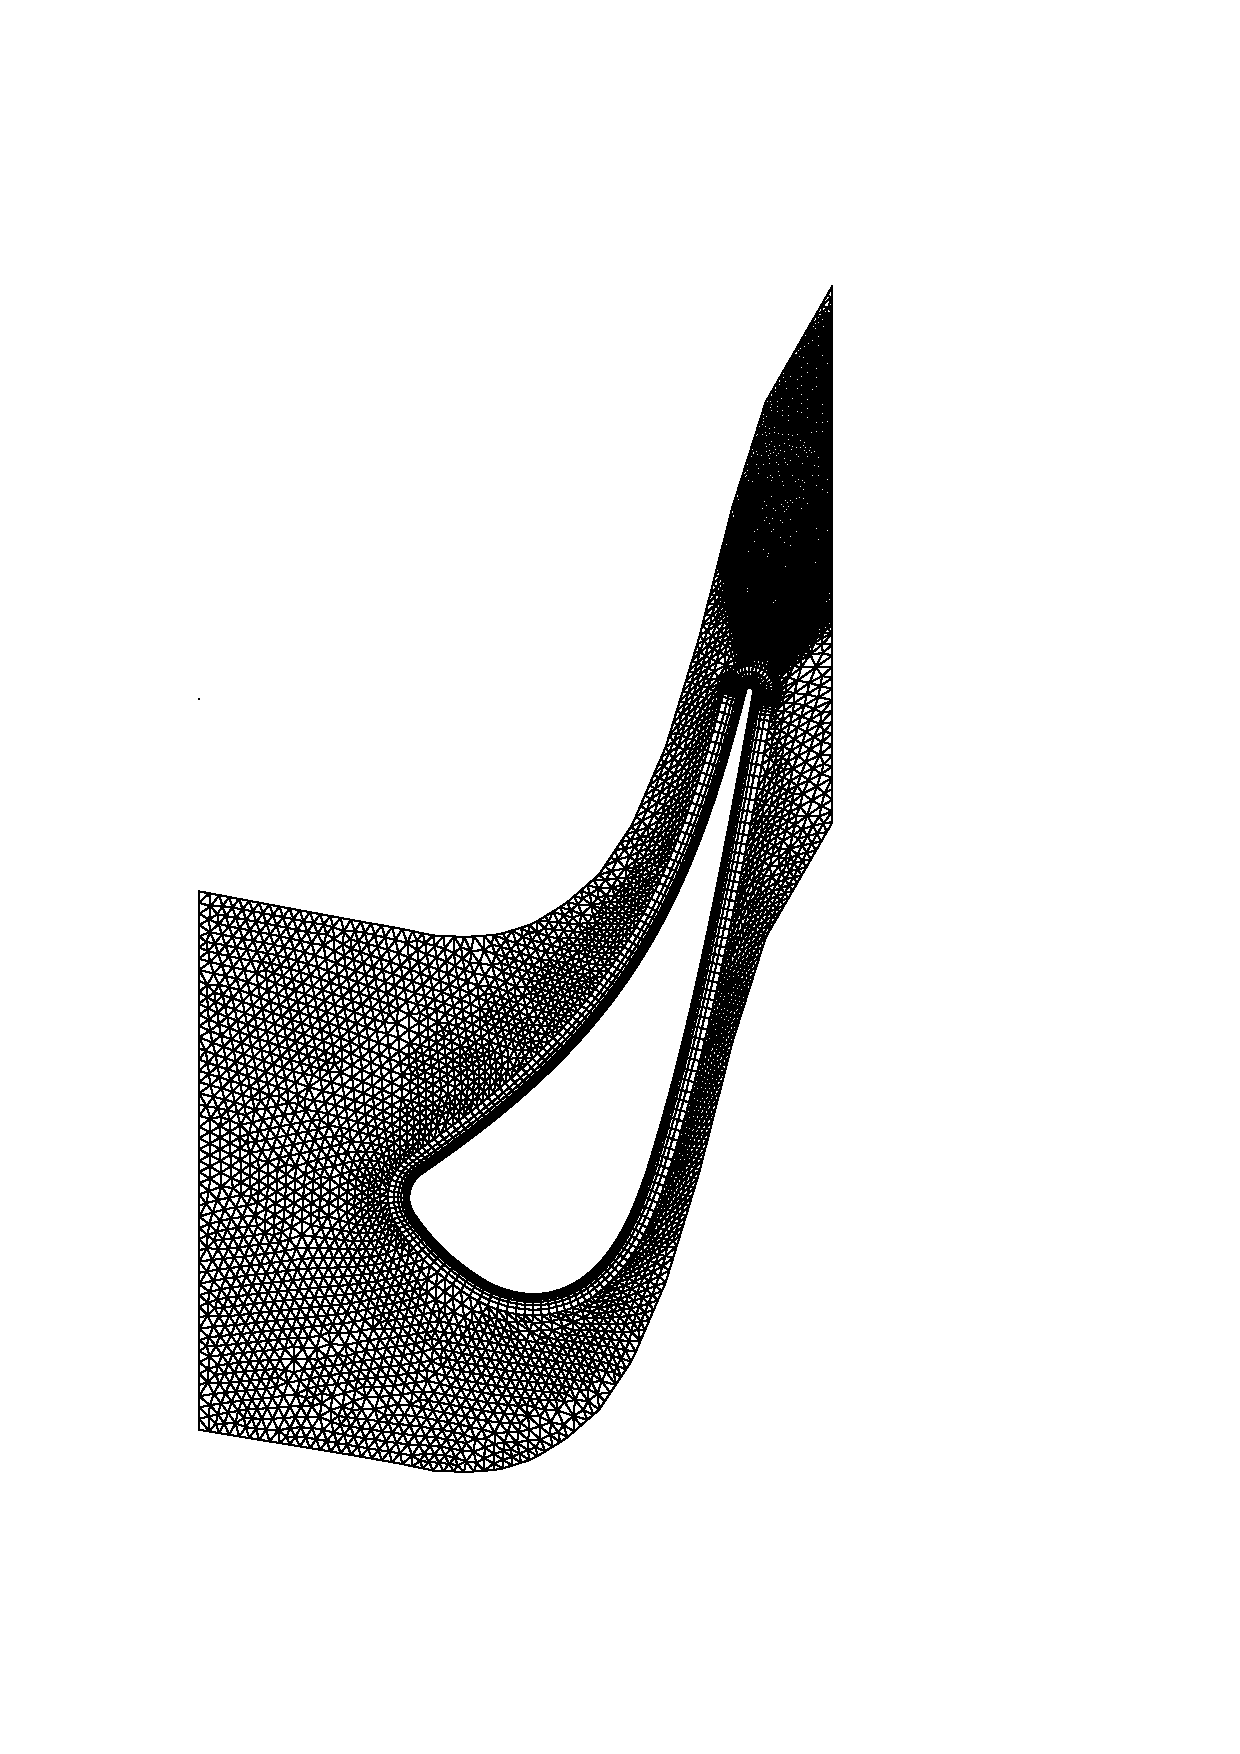
\includegraphics[width=45mm,clip=t]{CHAP_MESH/FIGURE/mesh2d_3_unstruct.pdf}}
      \end{tabular}}
  \end{tabular}
 \end{center}
 \vspace{-5mm}
 \caption{Structured meshes for mapping and corresponding mapped unstructured meshes at three radial levels}
 \label{mesh2d_other.fig}
\end{figure}
%
 Once the unstructured mesh has been mapped to all radial blade surfaces,
 a prismatic mesh is obtained by simply connecting the
 corresponding points at consecutive levels. Moreover,
 in order to enhance the quality of the 3D mesh, a
 smoothing procedure is performed. This operation
 alters the positions of the interior nodes without changing
 the topology of the mesh.
 The element sides are considered as springs of stiffness proportional
 to the length of the side. The nodes are moved until the spring system
 is in equilibrium, the position of which is found by Jacobi
 iterations.
%
%
%
\section{The Program LEVMAP}
\headb{Semi-structured Mesh Generator}{The program LEVMAP}
%
 The semi-structured mesh generation technique proposed in this Chapter
 has been implemented in the program LEVMAP (LEVel MAPping) written in
 Fortran 90. The LEVMAP program became a standard facility not only
 at the Vibration Centre but also at major aeroengine
 manifacturer. It is now used by
 many researchers and engineers for aerolasticity
 calculations on turbomachinery blades.
%
\begin{figure}[ht]
   \centerline{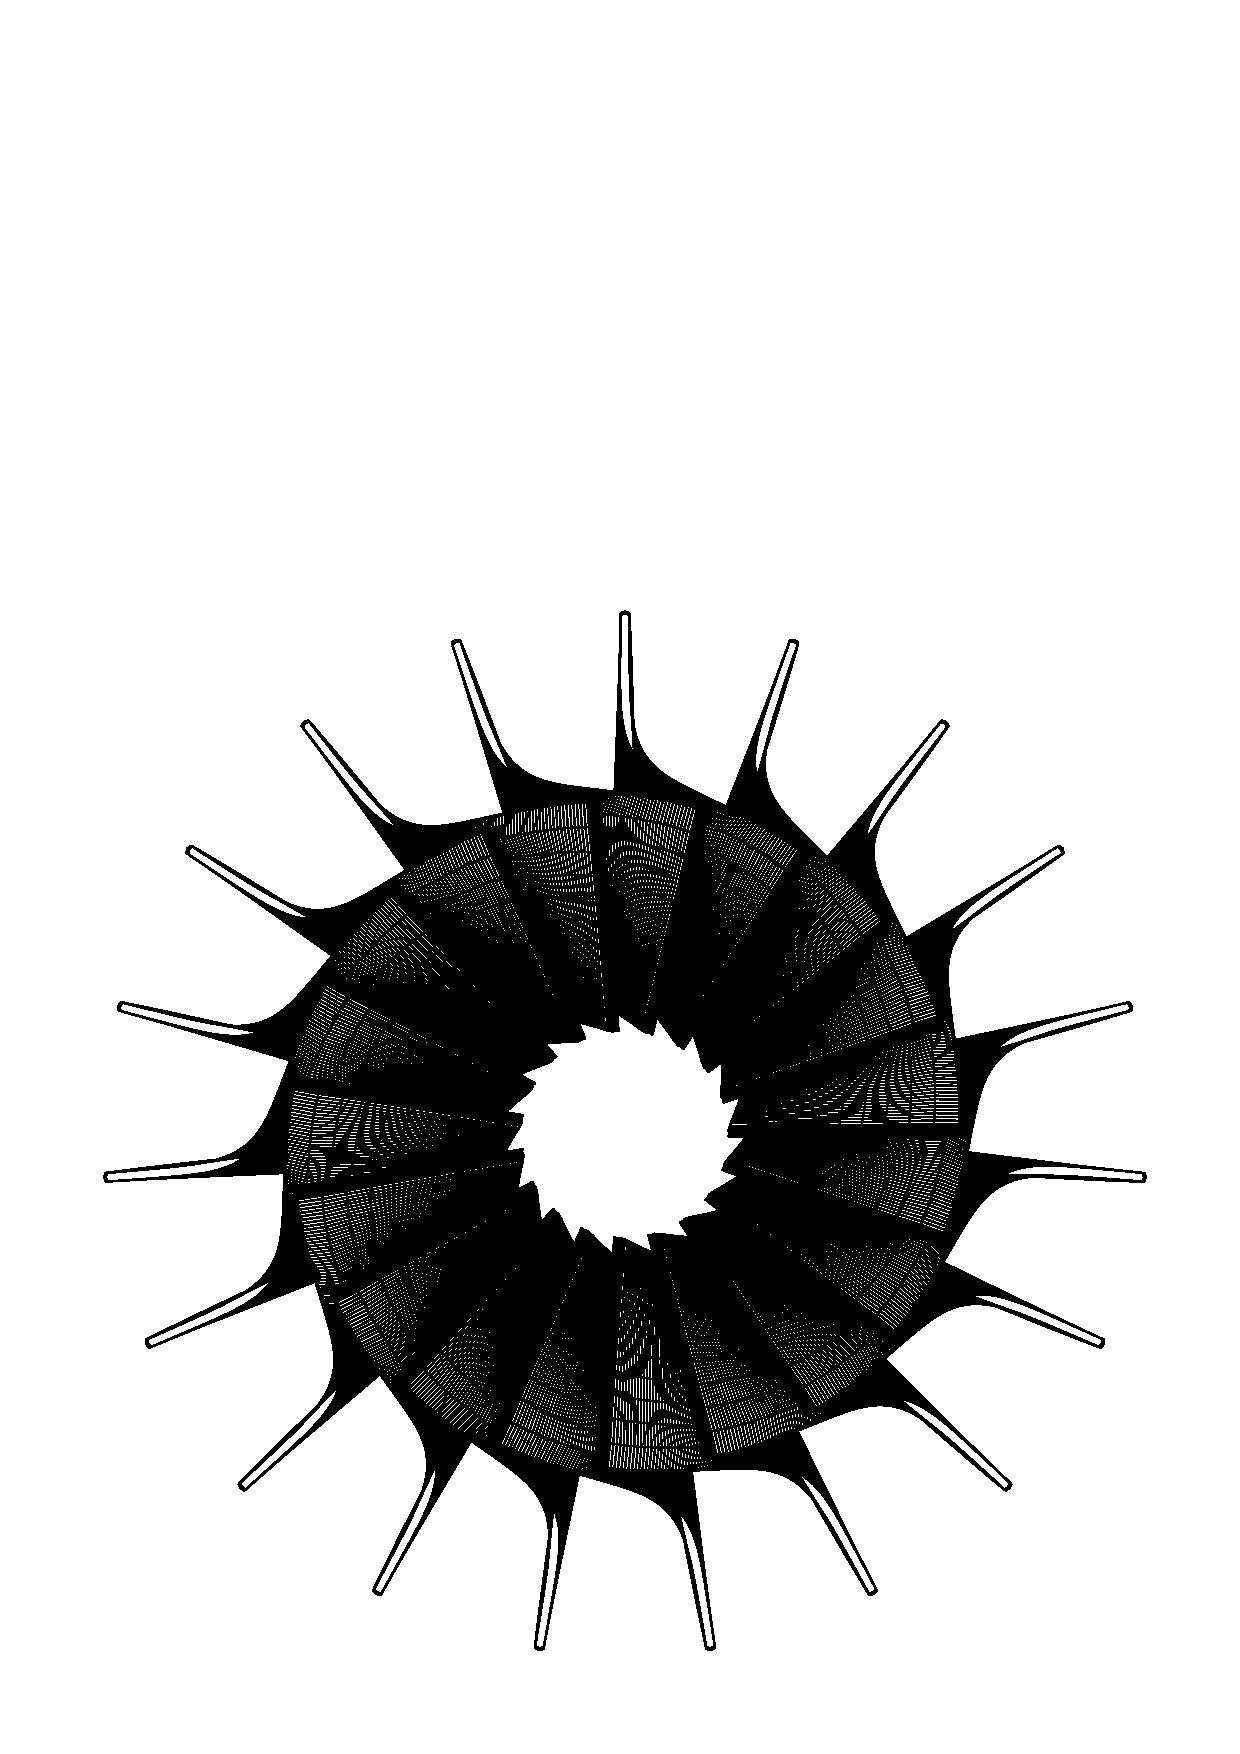
\includegraphics[width=140mm,clip=t]{CHAP_MESH/FIGURE/radial.pdf}}
   \caption{Semi-structured mesh for a radial-flow turbomachine}
   \label{radial_flow.fig}
\end{figure}
%
 A user's guide is available for the second release of the program
 (Sbardella \citeyearNP{Luca:5}).
 Grosclaude et al. \citeyear{Luca:8} extended LEVMAP to radial-flow
 turbomachine blades by modifying the 3D to 2D projection of
 Section \ref{geometry_modelling.sec}. An example of a semi-structured mesh
 for a radial turbomachinery assembly is shown in Fig. \ref{radial_flow.fig}.
 Further improvements of LEVMAP include automatic meshing of
 fan assembly + intake-duct, non-axisymmetric hub and tip, hub gap and
 snubber blades.
 Fig. \ref{snab_flow.fig} shows an exemple of semi-unstructured mesh for
 a snubbered fan blade assembly.
%
\begin{figure}[ht]
   \centerline{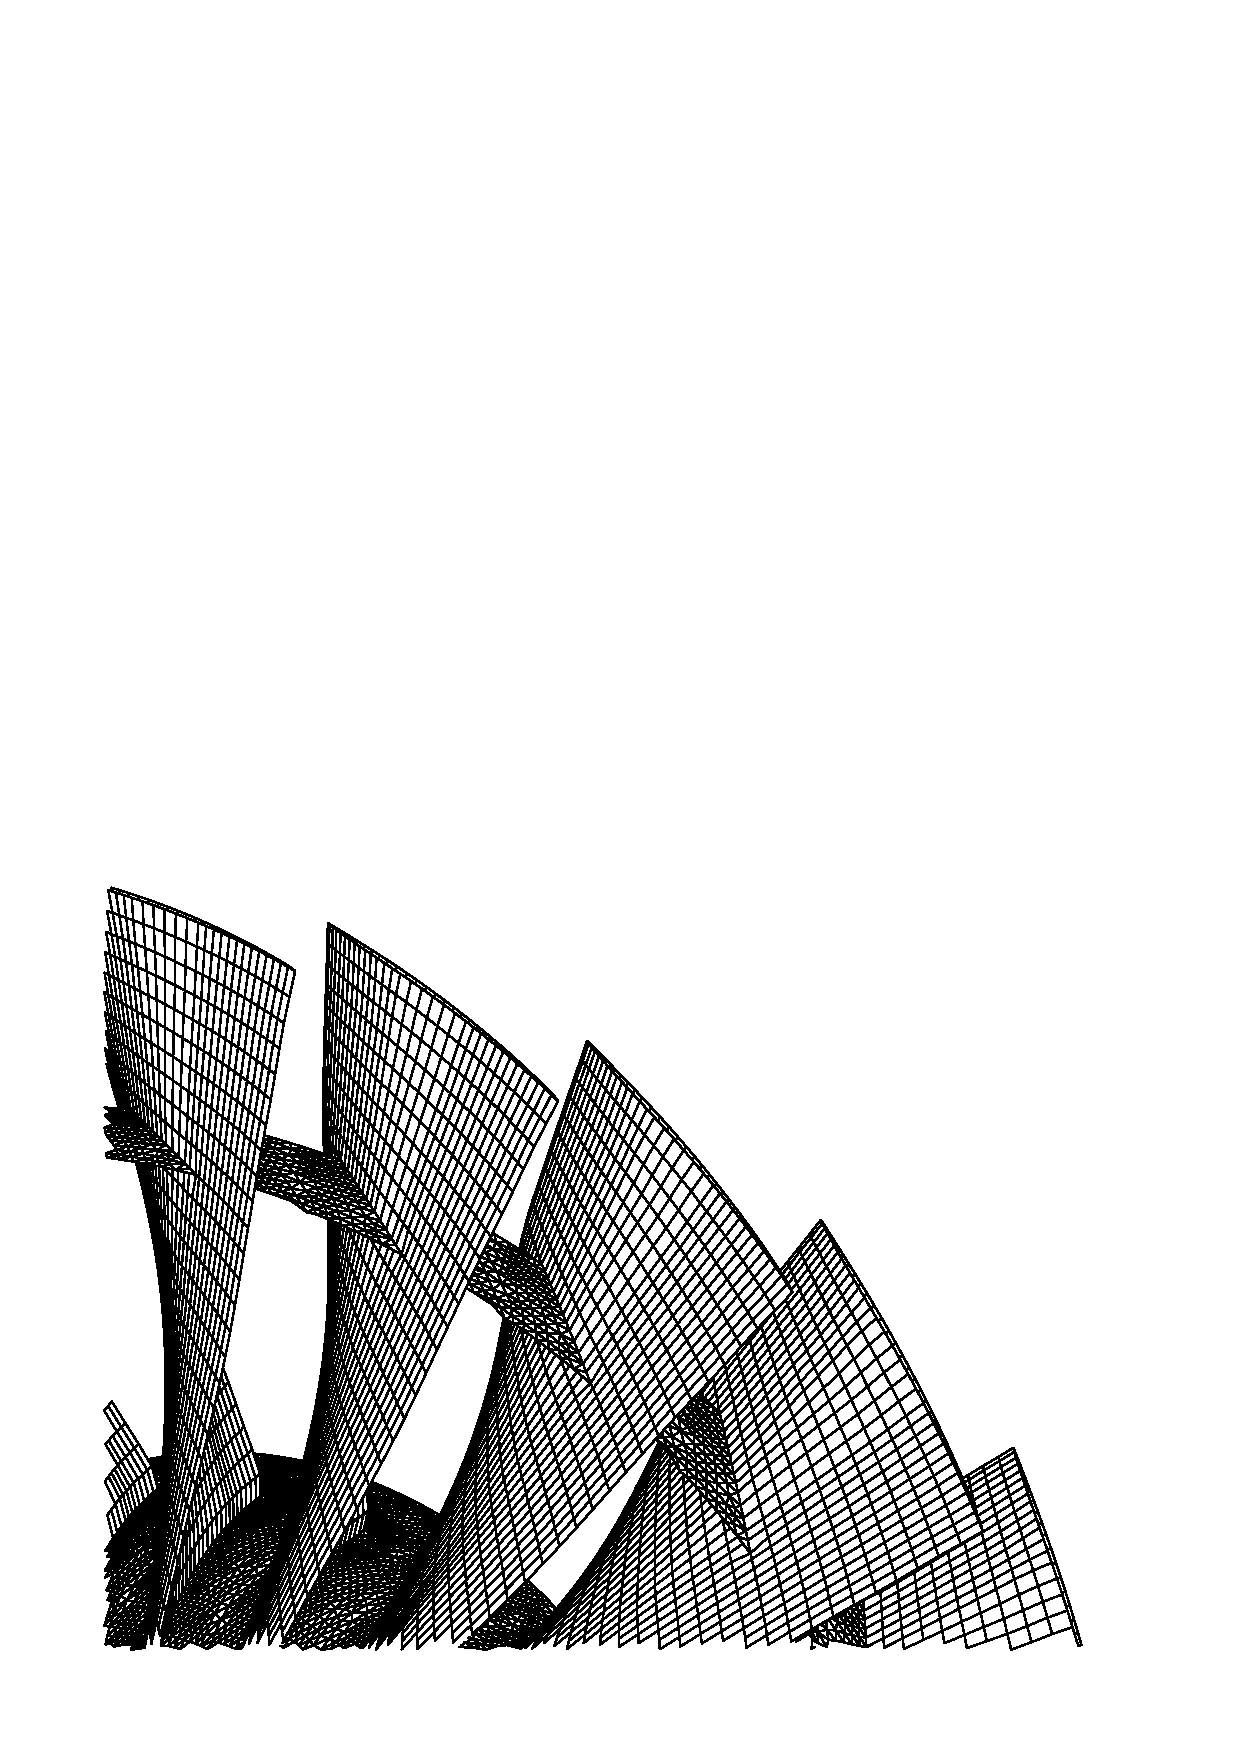
\includegraphics[width=120mm,clip=t]{CHAP_MESH/FIGURE/snab.pdf}}
   \caption{Semi-structured mesh for a snubbered fan assembly}
   \label{snab_flow.fig}
\end{figure}
%
%
%
%%%%%%%%%%%%%%%%%%%%%%%%%%%%%%%%%%%%%%%%%%%%
%%%%%%%      CONCLUDING REMARKS
%%%%%%%%%%%%%%%%%%%%%%%%%%%%%%%%%%%%%%%%%%%%
%
\section{Concluding Remarks}
\headb{Semi-structured Mesh Generator}{Concluding Remarks}
%
 A method to generate semi-structured prismatic meshes for turbomachinery
 blades has been presented. The unstructured mesh in the axial and
 tangential directions offers
 more flexibility than standard structured H-type, O-type and C-type meshes,
 both in terms of skewness minimization and smoothness optimization.
 The use of fully unstructured viscous meshes for blade like geometries
 is likely to require a much larger number of grid points and hence there
 are distinct advantages in using semi-structured meshes.
 Such was the success of the method that it was adopted by a major aeroengine
 manifacturer within one year of it being available.

%
%
%
%%%%%%%%%%%%%%%%%%%%%%%%%%%%%%%%%%%%%%%%%%%%%%%%%%%%%%%%%%%%%%%%%%%
\chapter{Hybrid Grid Solver for Turbulent Viscous Flow}
\label{flow_model.chap}
\heada{Hybrid Grid Solver for Turbulent Viscous Flow}
\setcounter{footnote}{0}
%%%%%%%%%%%%%%%%%%%%%%%%%%%%%%%%%%%%%%%%%%%%%%%%%%%%%%%%%%%%%%%%%%%
%
%
%
 This chapter presents a method for solving steady and unsteady, compressible,
 turbulent viscous flows for 2D and 3D turbomachinery blades.
 The flow model is based on the Favre-averaged Navier-Stokes equations,
 together with a one equation turbulence model.
 The space discretisation uses a node-centered finite volume scheme
 on unstructured mixed element grids, consisting
 of triangles and quadrilaterals in 2D, and of tetrahedra, pyramids, 
 triangular prisms and hexahedra in 3D. 
 The important features of the present approach are the 
 discretisation of the domain via a single, unified {\em edge-data structure}
 for mixed-element meshes and the use of a Laplacian weight
 which results in nearest neighbour stencils.
 The Laplacian weight is evaluated using an approximation of the
 Galerkin finite element method.
 In order to allow a straightforward implementation of fluid-structure
 coupling, the numerical solution is based on the Arbitrary
 Lagrangian-Eulerian method in which the grid points may be moved
 in an arbitrary but specified way.
 The pseudo time integration for steady-state problems is obtained using a
 preconditioned agglomeration multigrid method designed for highly
 anisotropic unstructured hybrid grids.
 In order to use the same preconditioned multigrid
 algorthim employed in the steady-state cases,
 a dual time-stepping technique is used for unsteady computations.
%
%
%
%
%
%
%
\section{Introduction}
\label{intro_nonlinear.sec}
\headb{Nonlinear Navier-Stokes solver}{Introduction}
%
 Over the last decade, significant advances have been made
 in the area of turbulent-viscous simulations using unstructured
 grids.
 However, compared with their structured counterparts,
 standard unstructured grid solvers have lower computational
 efficiency in terms of speed and storage.
 Unstructured grids often use tetrahedral elements only,
 an approach which often leads to numerical problems when the region to be
 discretised has a preferred direction such as the boundary layer for a
 high-Reynolds number flow. However, there are no fundamental difficulties in 
 extending tetrahedral meshes to include further element types such as triangular prisms, 
 pentahedra and hexahedra.  
 Although both the discretisation of the computational domain and the flow solver
 will become more complex,  such a mixed-element approach will offer
 a better, more efficient approximation than using tetrahedral elements only.
 For instance, hexahedral elements will handle boundary layer flows much better
 than tetrahedral elements because they can be made very slender without
 creating excessively small internal angles. 
 In order to handle mixed-element meshes, the spatial discretisation
 of the governing equations needs to be formulated in such a way
 that the numerical algorithms can be applied in a uniform way to all
 element types.
 A relatively simple way of achieving such consistent numerical treatment
 is to employ an edge-based data structure, which can be obtained
 from either a finite volume (FV) or a finite element (FE) formulation
 if the mesh consists of tetrehedral elements only. In this particular case, 
 all nodes are connected directly without any internal diagonals.
 However, quadrilaterals in 2D and hexahedrals in 3D have not only
 edges but also diagonal links. Therefore, to create an edge-based
 data structure from mixed meshes, one cannot use a FE technique
 because of the non-zero shape function contributions from the
 diagonally-opposed nodes for which there are no direct edges.
 Consequently, we will use a FV technique to obtain an edge-based
 data structure from mixed element meshes but, as reported by
 Barth \citeyear{Barth:4}, Parthasarathy et al. \citeyear{Kallinderis:2},
 Mavriplis \& Venkatakrishnan \citeyear{Mavriplis:3}
 for unstructured meshes of tetrahedra, 
 the discretisation of the viscous terms, remains a major problem. 
 The FV edge-based data structure is usually obtained by
 discretising the viscous terms in two sequential  loops, the so-called
 two-loop approach. The first loop is used to construct the gradients
 at all points, and the second one forms the second derivatives from
 the computed gradient information.
 Using such a technique, 
 the viscous fluxes are treated in an analogous manner to
 the inviscid ones and no extra storage is required.
 However, this strategy, used by several authors
 (see Peraire et al. \citeyearNP{Peiro:2}, Vahdati \& Imregun \citeyearNP{Mehdi:3})
 has at least three serious drawbacks.
 First, the {\em odd-even decoupling} can destabilize
 the numerical scheme in regions where the viscous effects are
 important, e.g. the boundary layer.
 Second, for a 1D mesh of spacing $h$, the scheme will reduce to a second
 difference on a stencil of $2h$, a feature which will lower numerical
 accuracy.  Since packing enough points into the viscous layer
 is one of the main difficulties associated with viscous flow
 computations, a scheme that operates on every other point is highly
 undesirable.
 The third problem is the difficulty of implementing a viscous Jacobian which
 becomes important if an implicit time integration scheme is employed.

 An alternative approach, based on Galerkin
 finite element (GFE) approximation where velocity
 and temperature are made dependent variables,  is the derivation of the six node-pair
 coefficients for the Hessian matrix (Mavriplis \citeyearNP{Mavriplis:4},
 Selmin \& Formaggia \citeyearNP{Formaggia}).
 Each coefficient  is associated with  two nodes only, hence the term "node-pair GFE". 
 As mentioned earlier, such a formulation is not edge-based for non-tetrehedral meshes because 
 of the possible diagonal links between the nodes of a hexahedral element.
 On the other hand, the final discrete viscous
 terms of such a GFE formulation form a nearest neighbour stencil.
 Therefore, using the  Hessian node-pair
 coefficients, six second derivatives can be calculated for each node.
 Since the viscous terms can be expressed as a summation of the product
 of the node-pair coefficients and the unknowns,
 the construction of a viscous Jacobian becomes straightforward by explicit
 differentiation. Furthermore, the odd-even decoupling is avoided and the accuracy is improved.
 Unfortunately, this approach needs additional storage for the six node-pair
 coefficients and its applicability is restricted to triangular/tetrahedral
 elements if an edge-based data structure needs be employed.

 In summary, when dealing with mixed-element meshes, FV formulations can
 yield edge-based data structures but viscous flux discretisation
 remains problematic. On the other hand, GFE formulations are more
 efficient but the edge-based data structure cannot be preserved for non tetrahedral elements.  
 Therefore, the discretisation of the viscous fluxes
 can be improved by combining  the
 storage efficiency of the two-loop FV approach  with the
 numerical efficiency of the node-pair GFE method in an edge-based FV framework.

%
%
\section{Favre Averaged Navier-Stokes Equations}
\label{mathematical_model.sec}
\headb{Nonlinear Navier-Stokes solver}{Flow equations}
%
 The system of Navier-Stokes equations constitute the most complete
 description of viscous, heat-conducting flows and represents the highest
 level of approximation for continuous fluids.
 However, from the point of view of computational fluid dynamics,
 the vast majority of flow situations occurring in engineering
 applications enter into a particular form of instability, called
 {\em turbulence}.
 This occurs in most flow situations when the inertial forces
 exceed the viscous forces by more than four orders of magnitude
 (the ratio of these two forces is called {\em Reynolds number}).
 This form of instability can be represented by statistical
 fluctuations of the flow quantities around mean or averaged values.
 Moreover, the space scale of these fluctuations is so small that their
 direct calculation is beyond the reach of computational capabilities
 for engineering applications.

 Therefore, time-averaged Navier-Stokes equations need to be considered
 in most situations.
 In the case of compressible flow equations, this averaging
 is called Favre averaging (Wilcox \citeyearNP{Wilcox}).
 Because of the non-linearity of the Navier-Stokes equations, this
 procedure generates additional unknowns which will be solved using a
 suitable turbulence model. 
 In this work, the Spalart Allmaras \citeyear{Spalart:1} one equation
 turbulence model has been used (Appendix \ref{turbulence.chap}).
%
%
%
%
\subsection{Mean flow equations}
\label{conservative_formulation.subsec}
%
%
 The unsteady, compressible, Favre-averaged Navier-Stokes
 equations for a blade row in 3D can be cast in terms of
 absolute velocity $\vec{v}$ but solved in a relative non-Newtonian reference frame
 rotating along with the blade about the $x$ axis with angular velocity
 ${\bf \Omega}$ as shown in Fig. \ref{axis.fig}.
 This system of equations, written in a dimensionless, Arbitrary
 Lagrangian-Eulerian (ALE), integral conservative
 form (Donea et al. \citeyearNP{Donea}) for a control
 volume ${\cal V}\left(t\right)$ with boundary
 ${\cal S}\left(t\right)$
 in Cartesian coordinates $\vec{x} = \left(x, y, z\right)$,
 takes the form
%
\beq
  \fpdt{} \int_{{\cal V}\left(t\right)} {\bf U} d{\cal V} +
  \oint_{{\cal S}\left(t\right)} \left[
  \vec{{\bf F}} \left({\bf U}, \vec{u}\right) -
  \frac{1}{Re}\vec{{\bf G}} \left({\bf U}, \nabla {\bf U}\right) \right]
  \cdot\vec{n}\, d{\cal S} =
  \int_{{\cal V}\left(t\right)} {\bf S}\,d{\cal V}
  \label{conservative_formulation_nl.eq}
\eeq
%
%
\begin{figure}[ht]
  \centerline{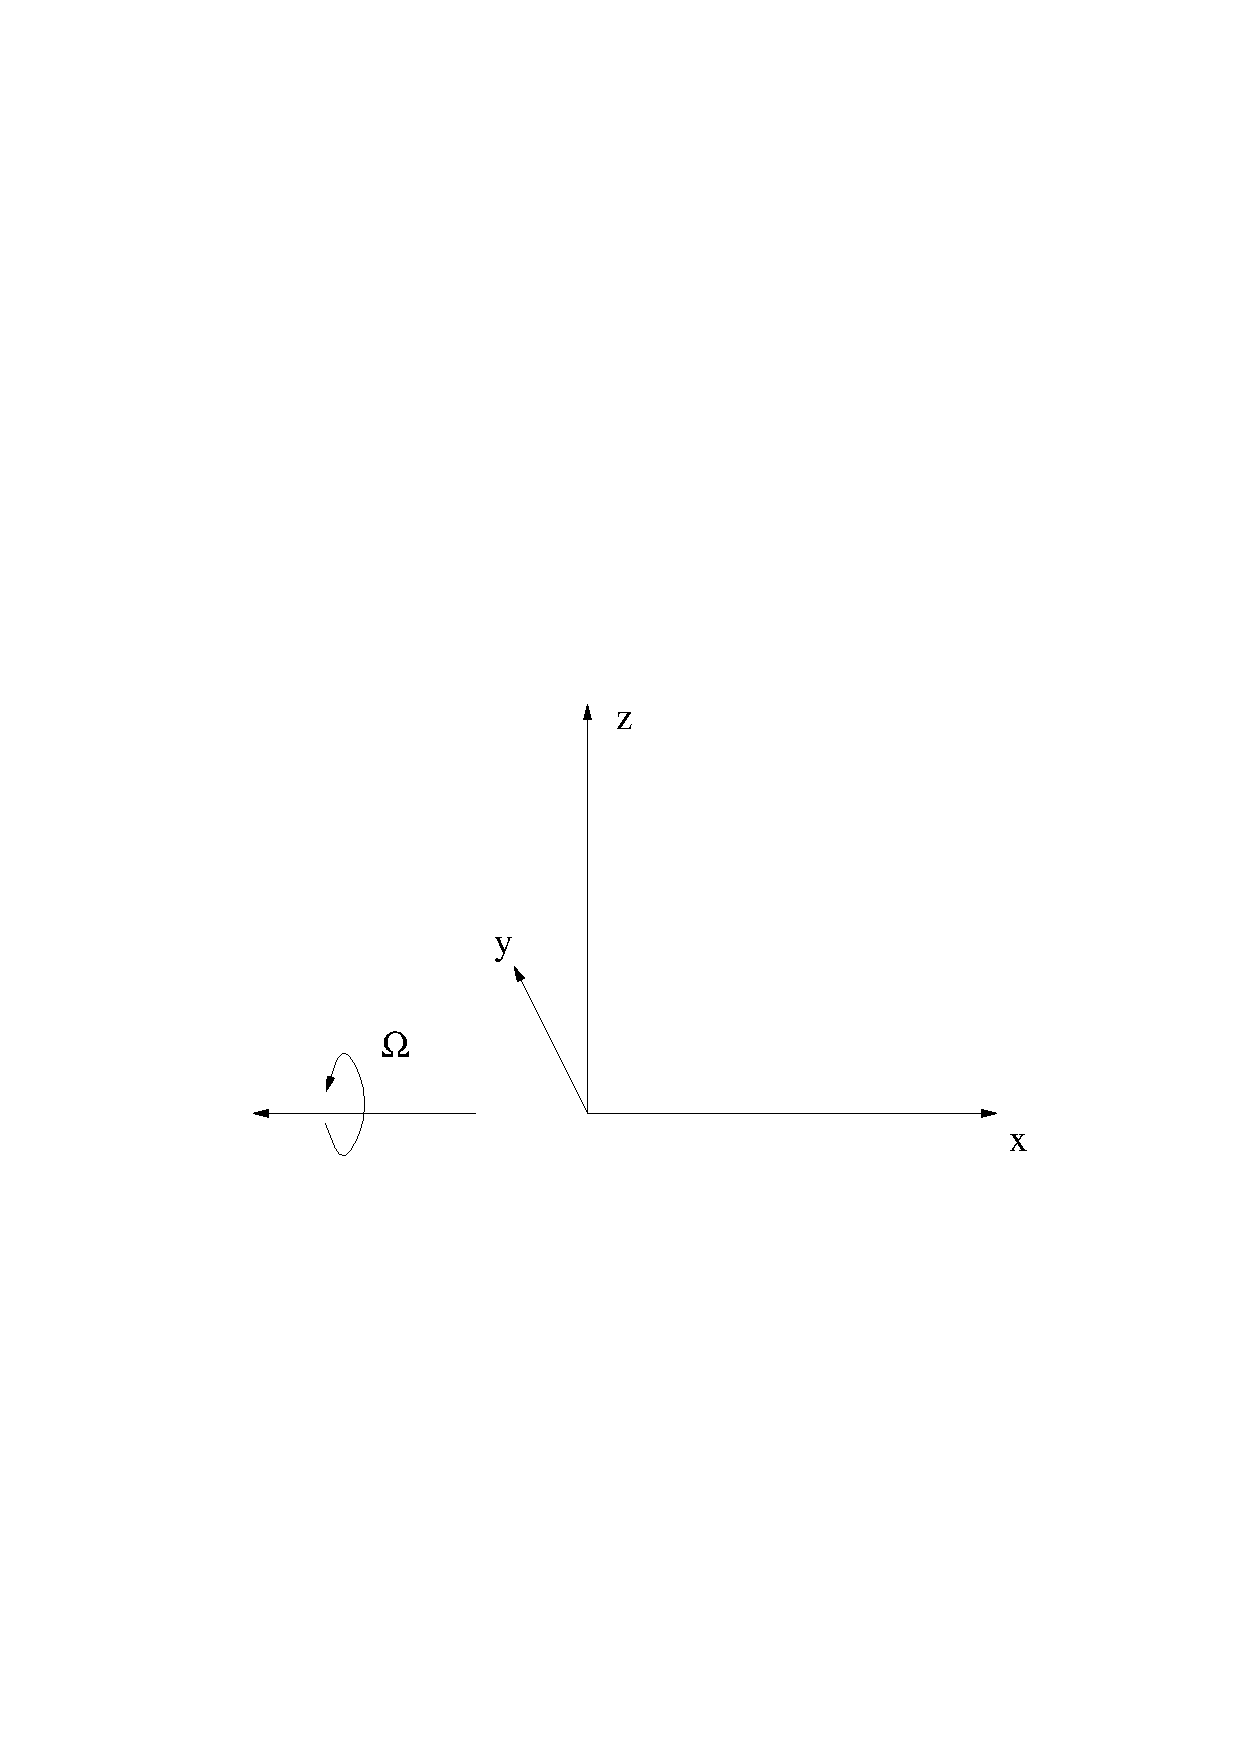
\includegraphics[width=60mm,clip=t]{CHAP_NONLIN/FIGURE/axis.pdf}}
  \caption{Direction of blade rotation}
  \label{axis.fig}
\end{figure}
%
 The viscous term $\vec{\bf G}$
 on the left-hand side of (\ref{conservative_formulation_nl.eq})
 is scaled by the reference Reynolds number so that flow variables are
 non-dimensionalised consistently. The dimensionless quantities are evaluated
 from their dimensional counterparts using the dimensional reference values
 reported in Appendix \ref{nondim.chap}.
 $\vec{n}$ represents the outward unit vector of the control volume boundary
 ${\cal S}\left(t\right)$. The vector $\vec{u}$, which represents the
 velocity in the relative frame of reference minus the velocity
 $\frac{d \vec{x}}{d t}$ of the boundary
 ${\cal S}\left(t\right)$, can be written as:
%
\beq
   \vec{u} = \vec{v} - \vec{\Omega} \times \vec{x} - \frac{d \vec{x}}{d t}
   \label{relative_velocity.eq}
\eeq
%
 where $\vec{\Omega} = \left(-\Omega,0,0\right)$. The sign of the angular velocity vector
 is determined by the assumption that the positive rotational speed is the
 one indicated in Fig. \ref{axis.fig}.
 The solution vector of conservative variables ${\bf U}$ is given by:
%
\beq
   {\bf U} = \left[
   \begin{array}{ccccc}
   \rho & \rho v\sm{1} & \rho v\sm{2} & \rho v\sm{3} & \rho E
   \end{array}
   \right]\se{T}
   \label{conservative_variables.eq}
\eeq
%
 The inviscid flux vector  $\vec{{\bf F}}\left({\bf U}, \vec{u}\right)$
 has the following components\footnote{${\bf U}u\sm{j}$ represents the $j$ component
 of the convective flux, while ${\bf F}{\scriptstyle p}\sm{j}$ represents the $j$ component
 of the pressure flux.}:
%
\beq
   {\bf F}\sm{j} &=& {\bf U}u\sm{j} + {\bf F}{\scriptstyle p}\sm{j}
   \label{nonlinear_inviscid_flux.eq}\\
   {\bf F}{\scriptstyle p}\sm{j} &=&
   \left[
   \begin{array}{ccccc}
   0 & p\delta\sm{1j} & p\delta\sm{2j} & p\delta\sm{3j} & v\sm{j} p
   \end{array}
   \right]\se{T}
   \label{nonlinear_pressure_flux.eq}
\eeq
%
 where $\delta\sm{ij}$ represents the Kronecker delta function.
 The static pressure $p$ and the total energy $E$ are related, in
 a non-dimensional fashion, to the density
 $\rho$, absolute velocity $\vec{v}$ and total enthalpy $H$
 by the following two equations which assume perfect gas with a constant
 ratio $\gamma$ of specific heat.

%
\beq
  p = \left(\gamma - 1\right) \rho \left[E - \frac{\left|\vec{v}\right|\se{2}}{2}\right],
  \ \ \ \ \ \
  H = E + \frac{p}{\rho}
 \label{pressure_energy_relations.eq}
\eeq
%
 Following the approach of Sbardella \& Imregun \citeyear{Luca:7,Luca:11},
 the viscous part of the governing equations is split into
 two distinct components, namely:

%
\beq
 \vec{\bf G} = \vec{\bf G}{\scriptstyle l} + \vec{\bf G}{\scriptstyle m}
 \label{viscous_terms.eq}
\eeq
%
 where

%
\beq
 \vec{\bf G}{\scriptstyle l} = \left[
 \begin{array}{c}
  0 \\ \mu \nabl v\sm{1} \\
       \mu \nabl v\sm{2} \\
       \mu \nabl v\sm{3} \\
       \mu\sum\sm{j=1}\se{3} v\sm{j}\nabl v\sm{j}
      + \frac{\gamma}{\gamma\!-\!1}
       \left(\frac{\mu\sm{l}}{Pr\sm{l}}\!+\!\frac{\mu\sm{t}}{Pr\sm{t}}\right) \nabl T
 \end{array} \right]
 \label{mean_flow_laplacian.eq}
\eeq
%
 $T=p/\rho$ is the non-dimensional static temperature of the fluid.
 The $j$-component of the second term on the left-hand side of
 (\ref{viscous_terms.eq}) is:

%
\beq
 {\bf G}{\scriptstyle m}\sm{j} = \left[
 \begin{array}{c}
  0 \\ \mu \fpd{v\sm{j}}{x\sm{1}} +
       \left(\lambda\nabl\cdot\vec{v}\right)\delta\sm{1j}\\
       \mu \fpd{v\sm{j}}{x\sm{2}} +
       \left(\lambda\nabl\cdot\vec{v}\right)\delta\sm{2j}\\
       \mu \fpd{v\sm{j}}{x\sm{3}} +
       \left(\lambda\nabl\cdot\vec{v}\right)\delta\sm{3j}\\
       \mu\left(\vec{v}\cdot\nabl v\sm{j}\right) +
       \lambda v\sm{j}\left(\nabl\cdot\vec{v}\right)
 \end{array} \right]
 \label{mean_flow_mixed.eq}
\eeq
%
 In (\ref{mean_flow_laplacian.eq}) and (\ref{mean_flow_mixed.eq}),
 $\mu$ represents the total dynamic viscosity of the fluid and is given
 by the summation of the laminar (physical) dynamic viscosity $\mu\sm{l}$
 and the turbulent dynamic viscosity $\mu\sm{t}$.
 The value of $\lambda$ is given by the
 Stokes relation $\lambda = -\frac{2}{3} \mu$
 which is valid for the majority of the flow situations with the exception
 of very high temperature or pressure ranges.
 It is easily seen that the
 component $\vec{\bf G}\sm{l}$ in (\ref{mean_flow_laplacian.eq})
 includes  the Laplacian operators of the three velocity components and
 temperature only.
 The second component, $\vec{\bf G}\sm{m}$, contains the mixed derivative terms,
 while the vector of source terms ${\bf S}$ on the right-hand side of
 (\ref{conservative_formulation_nl.eq}) takes into accounts for the blade
 rotation

%
\beq
  {\bf S} = \left[
   \begin{array}{ccccc}
    0 & 0 & \rho \Omega v\sm{3} & -\rho \Omega v\sm{2} & 0
   \end{array}
   \right]\se{T}
   \label{source_term.eq}
\eeq
%
 The derivation of the constitutive relations of viscous flows is discussed
 in detail by Schlichting \citeyear{Schlichting} and White \citeyear{White:1}.

%
\subsection{Boundary conditions}
\label{boundary_conditions_nonlinear.subsec}
%
%
%
 For convection dominated phenomena, such as those described by the 
 compressible Navier-Stokes equations, the formulation of correct boundary
 conditions is extremely important and its impact on the numerical scheme
 is often dominating.
 The reason for this strong influence can be traced back to the physical nature of
 the convection propagation phenomena (Hirsh \citeyearNP{Hirsch:1}).
 If all the variables were known at a boundary from the knowledge of the
 physical input, there would be no difficulty; however this is generally not the
 case with hyperbolic systems of partial differential equations.
 The number of physical
 variables that can be freely imposed at a boundary is dependent on the propagation
 properties of the system and, in particular, on the information propagated from
 the boundary towards the inside of the flow region. These are known as
 {\em physical boundary conditions}. The remaing variables will depend on the
 details of the flow and are, therefore, part of the solution. However
 from a numerical point of view, information about all variables
 is required  at the boundary. This additional information gives rise to
 {\em numerical boundary conditions} (Hirsch \citeyearNP{Hirsch:1}).
 
 The presence of viscosity and heat conduction
 transforms the conservation laws of momentum and energy into second-order
 partial differential equations.
 The system of Navier Stokes equations is therefore an hybrid system consisting of
 parabolic momentum and energy equations and of a hyperbolic continuity equation.
 A direct consequence is the need for a greater number
 of physical boundary conditions when dealing with viscous flows instead of
 inviscid flows.
%
%
\paragraph{Flow-tangency.}
%
 Also known as the inviscid wall condition, this boundary condition at the solid walls
 is expressed by the requirement that there is no flow through the surface
 of the moving wall. Only one physical boundary condition can be imposed
 at this boundary because only the forward travelling acoustic wave is entering
 the domain. Mathematically, this condition is expressed by the vanishing of the
 velocity normal to the wall.

%
\beq
  \vec{u}\cdot\vec{n} = 0
  \label{flow_tangency1.eq}
\eeq
%
 Expressed in a {\em week sense}, i.e. through the fluxes, (\ref{flow_tangency1.eq})
 becomes:

%
\beq
 \oint\sm{wall}\vec{\bf F}d{\cal S} =
 \oint\sm{wall}\vec{\bf F}{\scriptstyle p}d{\cal S} =
 \left[
 \begin{array}{c}
 0 \\ p\ n\sm{1} d{\cal S}\\
      p\ n\sm{2} d{\cal S}\\
      p\ n\sm{3} d{\cal S}\\
      p\ \left(\vec{\Omega}\times\vec{x}+\frac{d \vec{x}}{d t}\right)\cdot\vec{n}d{\cal S}
 \end{array}
 \right]
  \label{flow_tangency2.eq}
\eeq
%
\paragraph{No-slip condition.}
%
%
 The no-slip condition at the solid walls is expressed by the requirement that the
 fluid velocity relative to the moving wall must be zero.
 Mathematically this can be expressed as:

%
\beq
  \vec{u} = \vec{v} - \vec{\Omega}\times\vec{x} - \frac{d \vec{x}}{d t} = 0
  \label{no_slip1.eq}
\eeq
%
 In addition to (\ref{no_slip1.eq}), an additional information is required
 due to the presence of the second derivative terms in the Navier-Stokes
 equations\footnote{The no-slip condition is valid for viscous flow only.}.
 Here this additional information is for an adiabatic wall

%
\beq
  \vec{n}\cdot\nabl T = 0
  \label{no_slip2.eq}
\eeq
%
%
\paragraph{Inflow and outflow boundaries.} 
%
 The quasi-3D non-reflecting boundary
 conditions developed by Saxer \& Giles \citeyear{Giles:7} are used
 for steady-state computations.
 These boundary conditions are obtained from a Fourier mode analysis
 of the linearised Euler equations at the far-field boundaries.
 Implemented in a turbomachinery environment, the approach assumes
 that the solution at the boundary is circumferentially decomposed into Fourier modes,
 the $0\se{th}$ mode corresponding to the averaged solution.
 The $0\se{th}$ mode is treated according to the standard 
 1D boundary condition (Thompson \citeyearNP{Thompson:1,Thompson:2})
 which allows the user to specify certain physical quantities at the boundaries.
 Such averaged quantities are:
%
\begin{itemize}
 \item
  {\bf Inflow:} stagnation temperature, stagnation pressure and flow angles.
 \item
  {\bf Outflow:} static pressure.
\end{itemize}
%
 The remaining part of the solution, represented by the sum of the harmonics,
 is treated according to the exact\footnote{The term exact refers to the
 solution of the linear problem. Since the linear problem is itself an approximation
 to the nonlinear one, there will be errors which are proportional to the square
 of the amplitude of the non-uniformities at the far-field boundaries.}
 2D theory of Giles \citeyear{Giles:5,Giles:6}.
 Since this method considers radial flow variations in the $0\se{th}$ mode only, it is
 called quasi-3D non-reflecting boundary conditions. In the absence of any radial
 variations, the boundary conditions are exact within
 the 2D linear theory.

 The  standard 1D characteristic boundary conditions of
 Thompson \citeyear{Thompson:1,Thompson:2} are used for 
 unsteady time-marching aerodynamics.
%
%
% 
\paragraph{Periodic boundaries.}
%
 Taking advantage of the edge-based data structure, the periodicity is handled in 
 a straightforward way as long as the points in the two periodic
 boundaries are located at same axial and radial coordinates.
%
\beq
  {\bf U}_{\theta_0 + \Delta \theta} = {\bf U}_{\theta_0}
\eeq
%

%
%
%
%
\section{Spatial Discretisation}
\label{space_discretisation_nl.sec}
\headb{Nonlinear Navier-Stokes solver}{Spatial discretisation}
%
 The development of a FV edge-based data structure
 for unstructured mixed-element meshes
 will now be described in detail.

%
\begin{figure}[ht]
\centerline{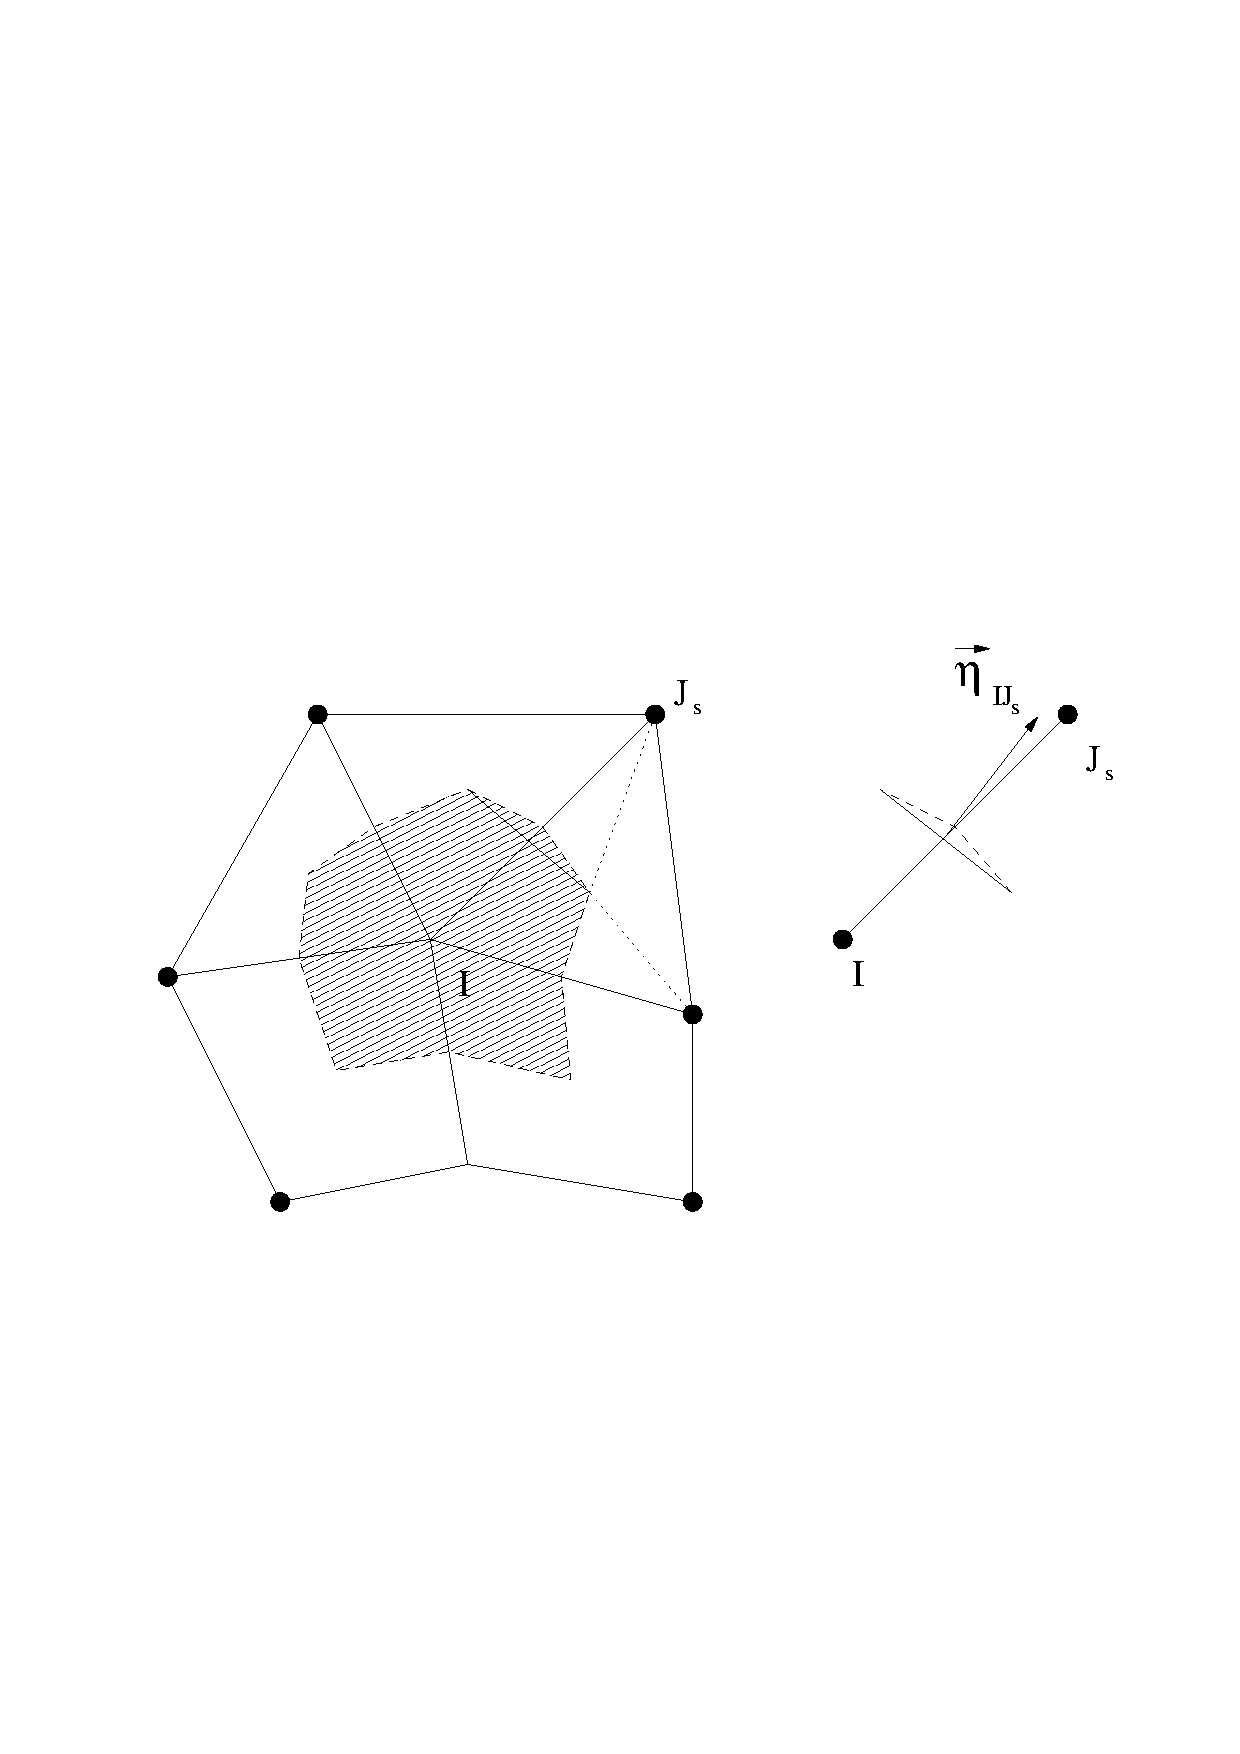
\includegraphics[width=80mm,clip=t]{CHAP_NONLIN/FIGURE/mixme.pdf}}
\caption{Control volume for node $I$ and metric vector
$\vec{\eta}\sm{IJs}$
 for edge $IJs$}
\label{median_dual.fig}
\end{figure}
%
 As shown for the 2D mesh of Fig. \ref{median_dual.fig},
 using a node-centered approach and choosing the median dual mesh as control
 volume\footnote{A discussion of different control volume definitions is
 given by Barth \& Jespersen 1989.},
 a FV discretisation of
 (\ref{conservative_formulation_nl.eq}), written
 in a semi-discrete form, is given by:

%
\beq
  \fpdt{\left({\cal V}\sm{I}{\bf U}\sm{I}\right)} &=& -\!
  \sum\sm{s=1}\se{m\sm{I}} \left[\left|\vec{\eta}\sm{IJs}\right|
  \left({\cal F}\sm{IJs}\!-\!{\cal G}\scriptstyle{m}\sm{IJs}\right)
  - \tau\sm{IJs} {\cal G}\scriptstyle{l}\sm{IJs}\right]
  + {\cal V}\sm{I}{\bf S}\sm{I}
  \label{semi_discrete_nl.eq}
\eeq
%
 As shown in Fig. \ref{median_dual.fig}, node $I$ is connected by edges to
 $m\sm{I}$ ($m\sm{I} = 6$ in Fig. \ref{median_dual.fig})
 nodes $J\sm{s}$, ${\cal V}\sm{I}$ representing the control volume
 associated with it.
 ${\cal F}$, ${\cal G}\scriptstyle{m}$ and ${\cal G}\scriptstyle{l}$
 correspond to the inviscid and viscous vectors $\vec{\bf F}$,
 $\vec{\bf G}\scriptstyle{m}$ and $\vec{\bf G}\scriptstyle{l}$.
 $\vec{\eta}\sm{IJs}$ is the metric vector associated with the
 surface area of edge $IJs$ while $\tau\sm{IJs}$ represents the Laplacian
 weight associated with the same edge.
 The summation in (\ref{semi_discrete_nl.eq}) has been obtained applying
 the Green's formula to the surface integral of (\ref{conservative_formulation_nl.eq})
 and choosing as path the median dual mesh (Barth \& Jespersen \citeyearNP{Barth:1},
 Barth \citeyearNP{Barth:2}).
 Of particular interest here is the use of the GFE node-pair formula
 for the Laplacian operator $\tau\sm{IJs}$ in order to construct
 an approximate version for the FV edge-data scheme
 (Sbardella \& Imregun \citeyearNP{Luca:7,Luca:11}).
%
%
%
%
%
\subsection{Inviscid discretisation}
\label{inviscid_disretisation.subsec}
%
 The discretisation of the inviscid flow terms in
 (\ref{semi_discrete_nl.eq}) is given by:

%
\beq
  \sum\sm{s=1}\se{m\sm{I}} \left|\vec{\eta}\sm{IJs}\right|
  {\cal F}\sm{IJs}
 \label{inviscid_contribution_nl.eq}
\eeq
%
 where ${\cal F}\sm{IJs}$ represents the inviscid flux function along edge
 $IJ\sm{s}$
 which is obtained using a central difference scheme with added
 matrix artificial dissipation. This artificial dissipation
 is a blend of second and fourth order differences. The fourth order
 terms ensure the stability of the scheme in smooth regions of the flow,
 while the second order terms are required to damp numerical oscillations
 in the vicinity of discontinuities.
 The inviscid flux function is expressed as:

%
\beq
  {\cal F}\sm{IJs} = \frac{\vec{\bf F}\sm{I}+\vec{\bf F}\sm{Js}}{2}
  \cdot\frac{\vec{\eta}\sm{IJs}}{\left|\vec{\eta}\sm{IJs}\right|}
  - {\cal D}\sm{IJs}
  \label{inviscid_flux_function_nl.eq}
\eeq
%
 where the artificial dissipation ${\cal D}\sm{IJs}$ along the edge is
 given by:

%
\beq
  {\cal D}\sm{IJs} = \frac{1}{2}
  \left|{\bf A}\sm{IJs}\right|
  \left[\psi\Delta{\bf U} - \epsilon\sm{4}\left(1-\psi\right)\Delta{\cal L}\left({\bf U}\right)\right]
  \label{artifical_diffusion_nl.eq}
\eeq
%
 Here $\Delta$ represents the difference operator along edge $IJs$

%
\beq
  \Delta\left(\cdot\right) = \left(\cdot\right)\sm{Js} -
\left(\cdot\right)\sm{I}
\label{difference_operator.eq}
\eeq
%
 $\left|{\bf A}\sm{IJs}\right|$ is the standard Roe matrix
 (Roe \citeyearNP{Roe:1})
 between the two stages ${\bf U}\sm{I}$ and ${\bf U}\sm{Js}$,
 $\epsilon\sm{4}\approx 1/16$ is the fourth order artificial dissipation
 coefficient. $\cal L\sm{I}\left({\bf U}\right)$ is a pseudo-Laplacian
 operator, at node $I$, given by:

%
\beq
  {\cal L}\sm{I}\left({\bf U}\right) =
  \left(\sum\sm{s=1}\se{m\sm{I}}
  \frac{{\bf U}\sm{Js}-{\bf U}\sm{I}}{s\sm{IJs}}\right)
  \left(\sum\sm{s=1}\se{m\sm{I}}
  \frac{1}{s\sm{IJs}}\right)\se{-1}
  \label{pseudo_lapl_nl.eq}
\eeq
%
 where

%
\beq
  s\sm{IJs} = \left|\vec{x}\sm{Js} - \vec{x}\sm{I}\right|
  \label{svalll.eq}
\eeq
%
 $\psi$ represents the limiter function which varies between
 0 and 1 and it is required in order to switch the scheme to first order
 ($\psi = 1$) in the vicinity of discontinuities (Jorgenson \&
 Turkel \citeyearNP{Turkel:2}).
%
%
\subsubsection{Evaluation of metric vector}
%
 The metric vector $\vec{\eta}\sm{IJs}$ is obtained
 via a summation of the two dual median lengths around the edges,
 multiplied by their normals. For example the metric vector of the edge
 connecting nodes $I$ and $Js$ is shown in Fig. \ref{median_dual.fig} for a
 2D mesh.
 Another way of calculating $\vec{\eta}\sm{IJs}$ is the use of the
 GFE scheme in a node-pair formulation
 (Selmin \& Formaggia \citeyearNP{Formaggia}):

%
\beq
  \vec{\eta}\sm{IJs} = \sum_{e \in IJs} \int\sm{{\cal V}\sm{e}}
  \left(N\sm{I}\nabl N\sm{Js} - N\sm{Js}\nabl N\sm{I}\right) d{\cal V}
  \label{inviscid_weigh.eq}
\eeq
%
 where $e \in IJs$ indicates the set of elements which
 share nodes $I$ and $Js$, and $N\sm{I}$ is the test function of
 the GFE method.
 In the derivation of (\ref{inviscid_weigh.eq}), no a-priori assumptions
 were made regarding element types or the space dimensionality of the flow.
 If the FE test function $N$ is linear,
 both FV and GFE schemes will result in the same neighbouring stencil
 on triangular and tetrahedral meshes.
 Since all nearest neighbours are joined to the vertex under consideration
 by an edge, the node-pair formulation
 of (\ref{inviscid_weigh.eq}) is equivalent to an edge-based data
 structure (Bath \& Jespersen \citeyearNP{Barth:1},
 Selmin \& Formaggia \citeyearNP{Formaggia}).
%
\begin{figure}[ht]
 \begin{center}
  \begin{tabular}{cc}
    \subfigure[Galerkin finite element (GFE)]
     {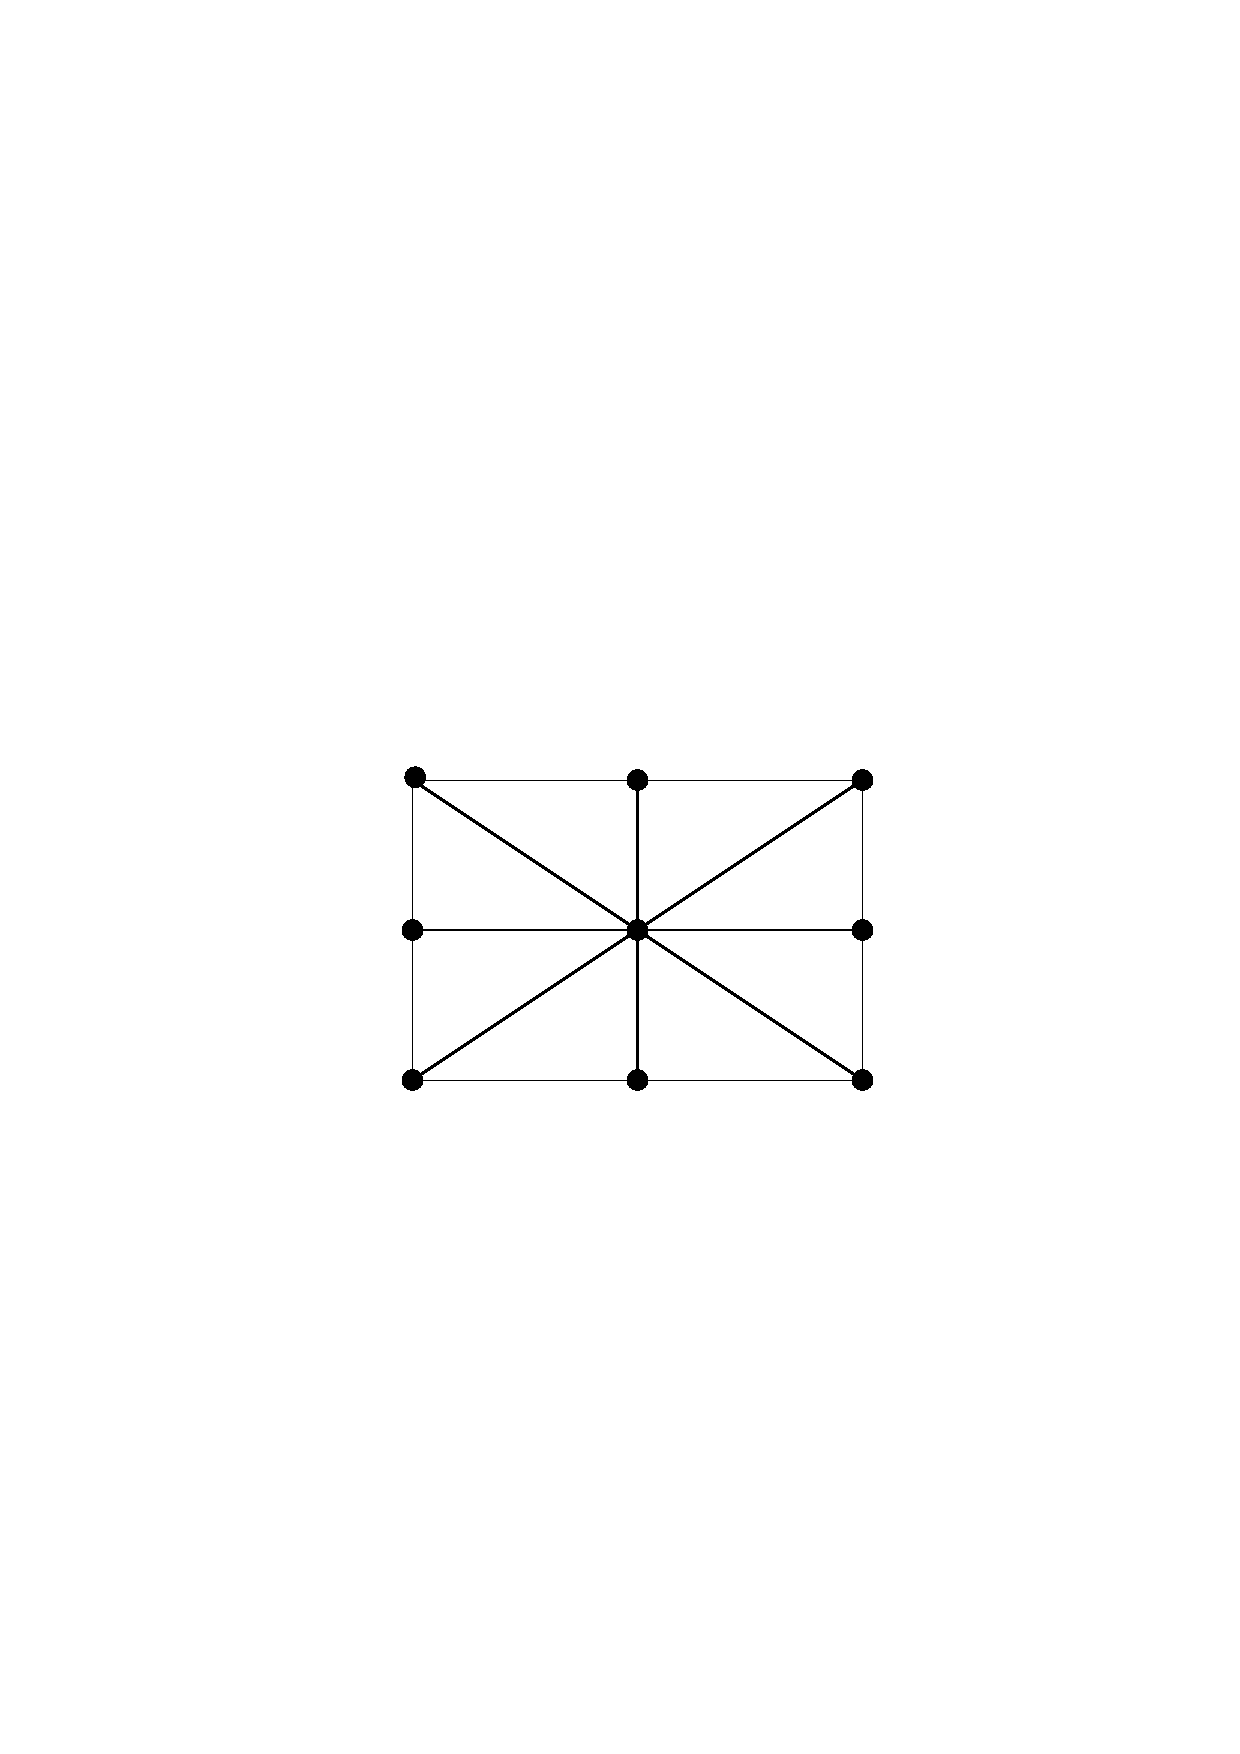
\includegraphics[width=60mm,clip=t]{CHAP_NONLIN/FIGURE/fe_quad_stencil.pdf}}
     &
    \subfigure[Finite volume (FV)]
     {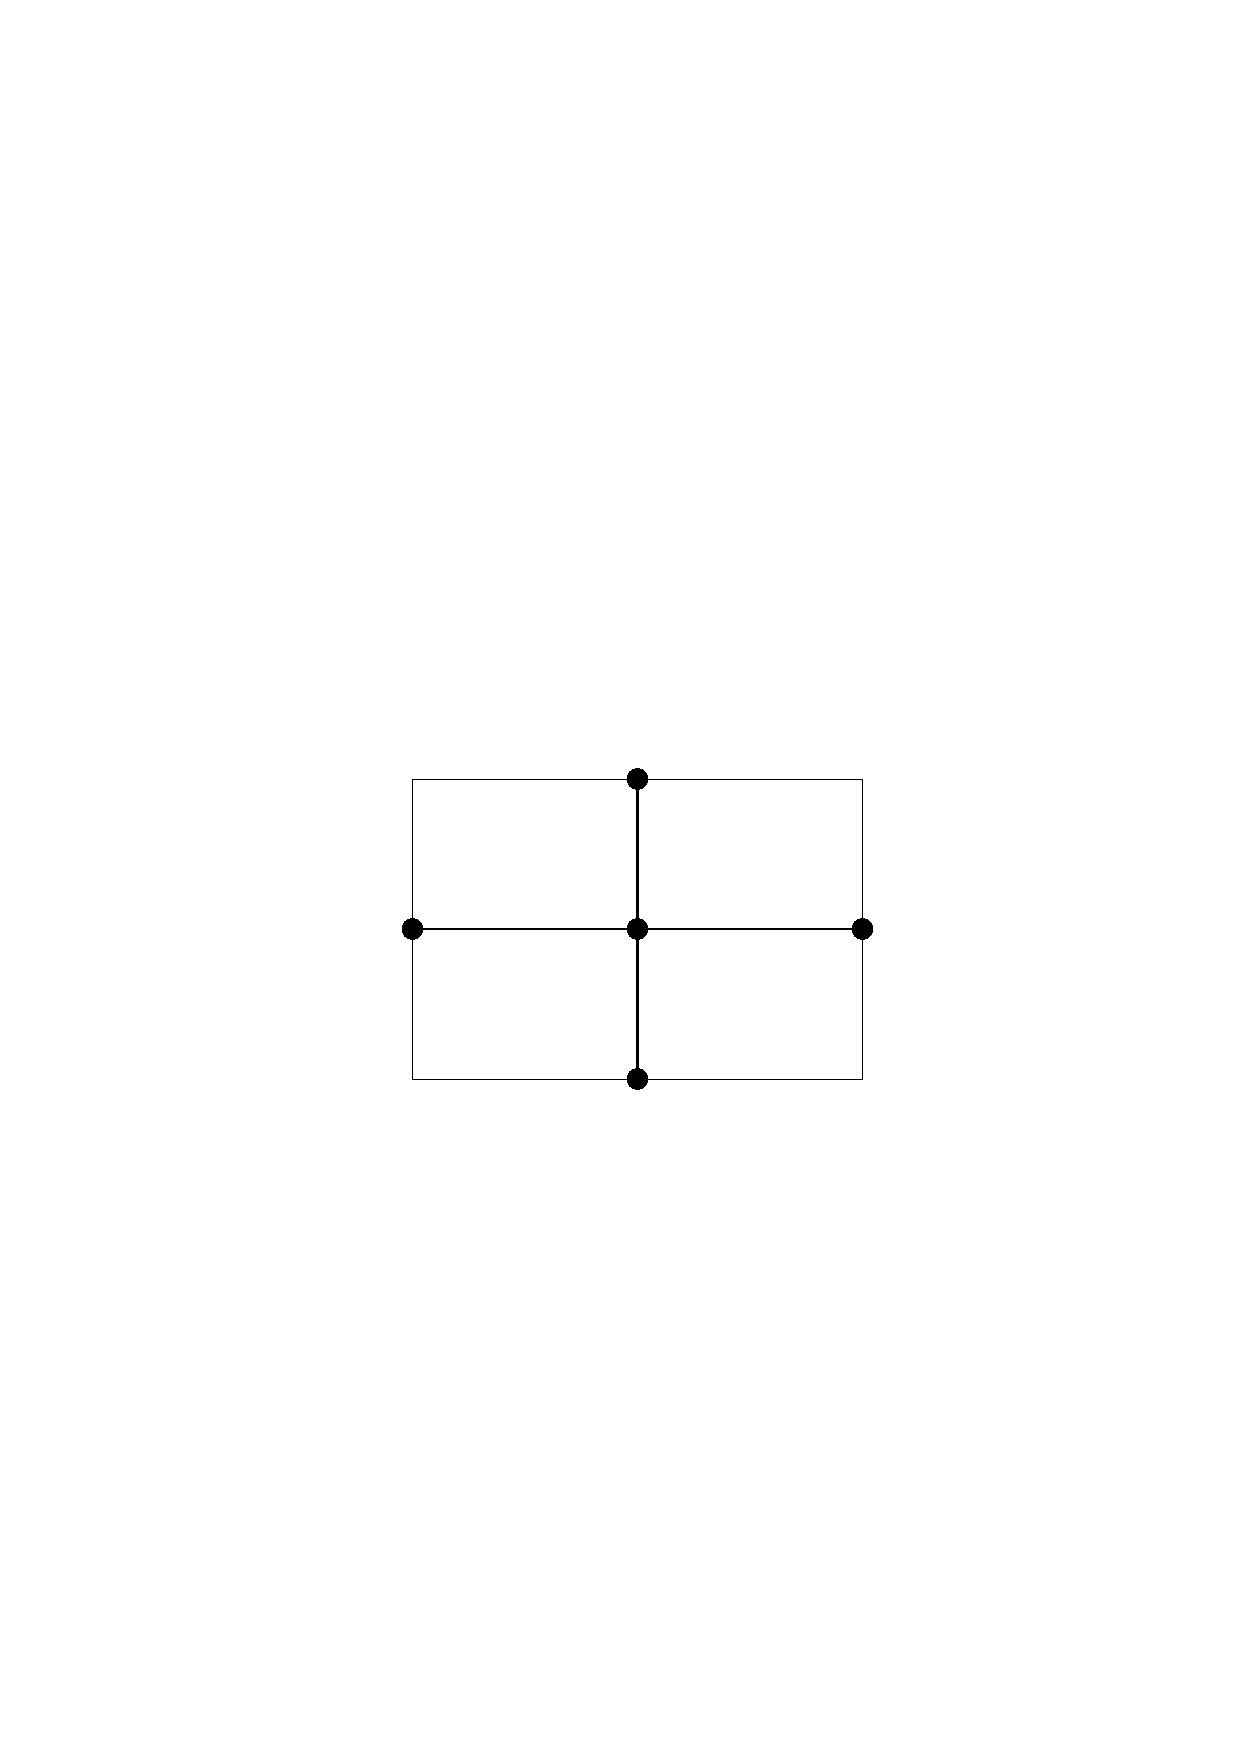
\includegraphics[width=60mm,clip=t]{CHAP_NONLIN/FIGURE/fv_quad_stencil.pdf}}
   \end{tabular}
  \end{center}
\vspace{-5mm}
\caption{Stencils for a quadrilateral mesh}
\label{fe_fv_quadrilateral.fig}
\end{figure}
%
 However, for quadrilaterals in 2D, and pyramids, wedges
 and hexahedra in 3D,
 the edge-data structure of a standard FV discretisation
 is no longer equivalent to the node-pair formulation of the GFE
 method.
 For example, in the case of a quadrilateral element, the GFE formulation
 takes into account the diagonal links. This approach results
 in a 9-point stencil, involving all corner points of the 4 quadrilaterals
 which share the vertex under consideration.
 On the other hand, the classical FV formulation considers the edge-based
 links only, resulting in a 5-point stencil (Fig. \ref{fe_fv_quadrilateral.fig}).
 Similarly, for a hexahedral element, the GFE method results in a 27-point
 stencil whereas the FV results in a 9-point stencil.
 Consequently, the GFE method is more expensive than the standard FV method
 but it has less dependence on mesh quality. For instance, when a mesh
 of quadrilateral or hexahedral elements is not orthogonal,
 the FV scheme still retains its conservation properties but its accuracy
 degenerates from second to first order (Essers at al. \citeyearNP{Essers:1}).
 For distorted meshes,
 the FV scheme is unable to recover the correct
 gradient values for a linear field on such elements. However, in the present
 formulation, the gradient information is used only
 for the evaluation of the limiter $\psi$
 in (\ref{artifical_diffusion_nl.eq}).
 By adopting a suitable limiter function, as that developed by Jorgenson \&
 Turkel \citeyear{Turkel:2},
 the FV scheme should retain its overall second order accuracy.
%
%
\subsubsection{Artificial dissipation and limiter function}
%
 Central-difference type schemes, such that in (\ref{inviscid_flux_function_nl.eq}),
 are commonly used for the solution of the Euler and Navier-Stokes equations.
 The artificial dissipation ${\cal D}\sm{IJs}$ in (\ref{artifical_diffusion_nl.eq})
 plays a crucial role in the determination of the quality of the numerical method.
 One of the first central-difference schemes used the
 scalar artificial dissipation model developed by Jameson et at.
 \citeyear{Jame:1}. During the 1980s, a considerable amount of research effort
 has been devoted towards the construction of more sophisticated
 schemes by minimising the added artificial dissipation.
 The paper by Swanson \& Turkel \citeyear{Turkel:1} summarises
 such effort and shows how central difference schemes
 with matrix artificial dissipation, as that in (\ref{artifical_diffusion_nl.eq}),
 are related to upwind schemes which utilize concepts from the characteristic
 theory in order to determine the direction of spatial differencing
 (Roe \citeyearNP{Roe:1}, Harten \citeyearNP{Harten:2}, Osher \citeyearNP{Osher:1},
 Pandolfi \citeyearNP{Pandolfi}, Roe \citeyearNP{Roe:2}).
 In fact, scheme (\ref{inviscid_flux_function_nl.eq}) with $\psi = 1$
 is equivalent to the first-order upwind scheme of Roe \citeyear{Roe:1}.
 Also, upwind schemes can be designed to have the TVD property
 in the case of scalar conservation laws
 (Harten \citeyearNP{Harten:1}, Osher \citeyearNP{Osher:2}).
 The TVD property is very useful in constructing limiter functions
 for second-order numerical schemes (Sweby \citeyearNP{Sweby:1}).
 Swanson \& Turkel \citeyear{Turkel:1} introduced flux limiter functions
 that are consistent with the central-difference dissipation models using the TVD
 property.

 The limiter function used here is a multidimensional extension
 of the modified, van Leer central difference limiter, proposed
 by Swanson \& Turkel \citeyear{Turkel:1}. For an equispaced
 1D mesh, the limiter function at point $I$ is defined as:

%
\beq
  \psi\sm{I} = \frac{\left|p\sm{I+1}-2 p\sm{I} + p\sm{I-1}\right|}
               {\left(1-\chi\right)\left(\left|p\sm{I+1}-p\sm{I}\right|+
                                     \left|p\sm{I}-p\sm{I-1}\right|\right)+
                         \chi\left(p\sm{I+1}+2 p\sm{I} + p\sm{I-1}\right)}
  \label{limiter.eq}
\eeq
%
 where $0 \leq \chi \leq 1$. If $\chi = 0$, $\psi\sm{I}$ becomes
 the van Leer central difference TVD limiter. If $\chi = 1$,
 $\psi\sm{I}$ is equivalent to that used  by Jameson et al.  \citeyear{Jame:1}.
 For a 3D mesh the limiter function associated with node $I$
 and side $IJs$ becomes:

%
\beq
  \left.\psi\sm{I}\right|\sm{IJs} =
  2\frac{\left| p\sm{Js} - p\sm{I} - \nabl p\sm{Js}\cdot\vec{s}\sm{IJs}\right|}
  {\left(1-\chi\right)
   \left(\left|p\sm{Js}-p\sm{I}\right|+
         \left|p\sm{I}-p\sm{Js}+\nabl p\sm{Js}\cdot\vec{s}\sm{IJs}\right|\right)
   + 2\chi\left(p\sm{Js}+p\sm{I}\right)}
  \label{limiter_mult_1.eq}
\eeq
%
 where $\vec{s}\sm{IJs}$ is given in (\ref{svalll.eq}).
 The final value of $\psi\sm{I}$ is than given by the maximum value
 of (\ref{limiter_mult_1.eq}) of all sides $IJs$ associated with node $I$:
%
\beq
  \psi\sm{I} = {\tt max}\left(\left.\psi\sm{I}\right|\sm{IJs}\right)
  \label{limiter_mult_2.eq}
\eeq
%
 The central-difference scheme in (\ref{inviscid_flux_function_nl.eq})
 is slightly more dissipative than a second-order upwind scheme and this
 is for two reasons. First
 $\psi\sm{I} = {\tt max}\left(\left.\psi\sm{I}\right|\sm{IJs}\right)$,
 is multidirectional, while $\psi\sm{I}$ is usually chosen along a particular
 direction in upwind schemes.
 Second, upwind limiters allow to have negative viscosity
 but still retaining the TVD property while central-difference scheme cannot
 have negative artificial dissipation.
 In any case, to compensate for this slight increase in dissipation,
 central-difference schemes are simpler to program and require
 less computer time per time step, especially if used in conjunction with
 multistage time stepping techniques where the artificial dissipation
 is evaluated at alternate stages (Appendix \ref{multigrid.chap}).
%
%
%
%
%
%
\subsection{Viscous discretisation}
\label{viscous_disretisation.subsec}
%
 The viscous fluxes associated with the mixed derivatives in
 $\vec{\bf G}\sm{m}$ of (\ref{mean_flow_mixed.eq})
 are treated in the same way as their inviscid
 counterparts and their contribution to (\ref{semi_discrete_nl.eq}) is given by:

%
\beq
  {\cal G}{\scriptstyle m}\sm{IJs} =
  \frac{1}{Re}\left(\vec{\bf G}{\scriptscriptstyle m}\sm{I} +
  \vec{\bf G}{\scriptscriptstyle m}\sm{Js}\right)\cdot
  \frac{\vec{\eta}\sm{IJs}}{\left|\eta\sm{IJs}\right|}
  \label{viscous_mix_nl.eq}
\eeq
%
 Here, the Laplacian terms will be treated in a novel way in order to
 improve both the accuracy and the robustness of the numerical scheme
 (Sbardella \& Imregun \citeyearNP{Luca:11}).
 In (\ref{semi_discrete_nl.eq}), these terms take the form:

%
\beq
 {\cal G}\scriptstyle{l}\sm{IJs} =
 \frac{1}{Re}\left[
 \begin{array}{c}
  0 \\ \mu\sm{IJs} \Delta v\sm{1}
    \\ \mu\sm{IJs} \Delta v\sm{2}
    \\ \mu\sm{IJs} \Delta v\sm{3}
    \\ \left(\mu \vec{v}\right)\sm{IJs}\cdot \Delta \vec{v} +
       +
\frac{\gamma}{\gamma\!-\!1}\left(\frac{\mu\sm{l}}{Pr\sm{l}}\!+\!
         \frac{\mu\sm{l}}{Pr\sm{t}}\right)\sm{IJs}\Delta T
 \end{array}
 \right]
 \label{bbbbbbbb.eq}
\eeq
%
 The subscript $IJs$ indicates an arithmetic mean over nodes $I$ and $Js$:
%

\beq
  \left(\cdot\right)\sm{IJs} =
  \frac{\left(\cdot\right)\sm{Js}+\left(\cdot\right)\sm{I}}{2}
  \label{side_average.eq}
\eeq
%
 The difference operator $\Delta$ in (\ref{bbbbbbbb.eq})
 is given in (\ref{difference_operator.eq}).
 In the present formulation, that deals with mixed-element meshes, the
 Laplacian weight $\tau\sm{IJs}$ in (\ref{semi_discrete_nl.eq}) is evaluated using
 an approximation of the GFE node-pair relation.
 For a generic 2D or 3D element, the GFE Laplacian weight can be written as
 (Selmin \& Formaggia \citeyearNP{Formaggia}):

%
\beq
  \tau\sm{IJs} = -\sum\sm{e\in IJs} \int\sm{{\cal V}\sm{e}}
  \nabl N\sm{I}\cdot\nabl N\sm{Js} d{\cal V}
  \label{laplacian_coefficient.eq}
\eeq
%
 As for (\ref{inviscid_weigh.eq}), the Laplacian node-pair coefficient
 can be used for triangle/tetrahedral elements only if the data structure
 is edge based.
 Equation (\ref{laplacian_coefficient.eq}) will now be extended to other types
 of elements so that an approximate Laplacian weight, that is suitable for an edge-data
 FV implementation, can be evaluated.
 Let us consider the quadrilateral element of Fig. \ref{laplacian.fig} to
 illustrate such an approach.
%
\begin{figure}[ht]
\centerline{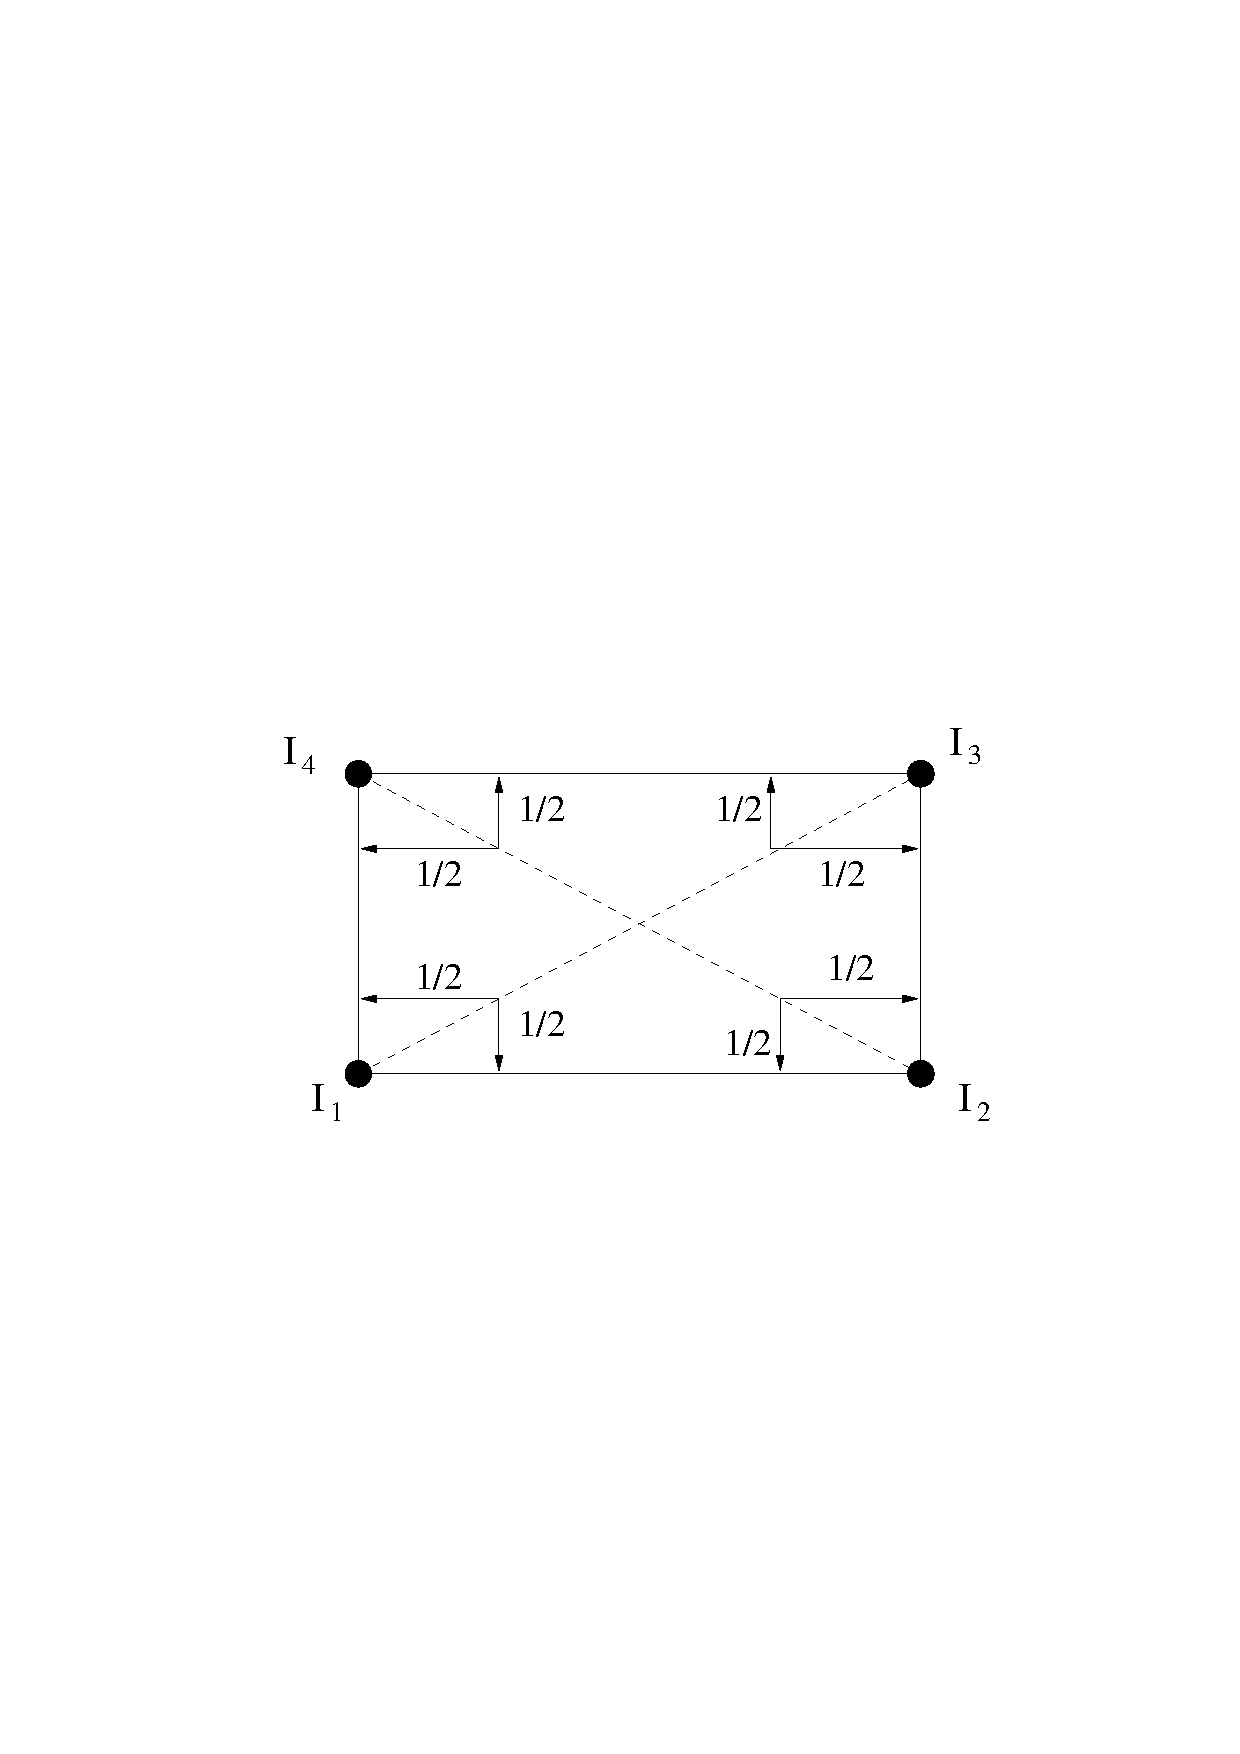
\includegraphics[width=60mm,clip=t]{CHAP_NONLIN/FIGURE/laplacian.pdf}}
\caption{Contribution of diagonal links to Laplacian weight for
         a quadrilateral mesh}
\label{laplacian.fig}
\end{figure}
%
 In (\ref{laplacian_coefficient.eq}), the two integrals involving the diagonal
 links between nodes ($I\sm{1} - I\sm{3}$) and  ($I\sm{2} - I\sm{4}$) are not zero.
 Since the diagonal links are not present in the FV formulation, in the present method
 their contribution is added to the edge links ($I\sm{1} - I\sm{2}$), ($I\sm{2} - I\sm{3}$),
 ($I\sm{3} - I\sm{4}$) and ($I\sm{1} - I\sm{4}$).
 As sketched in Fig. \ref{laplacian.fig}, each diagonal link contributes by
 a factor of 1/2 to the Laplacian operator of any of the four edges of
 the quadrilateral element.
 An equivalent treatment is adopted for pyramids, wedges and hexahedra.
 The integration of (\ref{laplacian_coefficient.eq}) is obtained using a
 one point Gauss quadrature for all type of elements.
 If the mesh is orthogonal, this approach will
 recover the second-order Laplacian weight of the GFE method.
%
%

%
%
%
%%%%%%%%%%%%%%%%%%%%%%%%%%%%%%%%%%%%%%%%%%%%%%%%%%%%%%%%%%%%%%%%%%5
%
%    TIME INTEGRATION
%
%%%%%%%%%%%%%%%%%%%%%%%%%%%%%%%%%%%%%%%%%%%%%%%%%%%%%%%%%%%%%%%%%%5
%
%
\section{Time Integration}
\label{time_integration_nonlinear.section}
\headb{Nonlinear Navier-Stokes solver}{Time integration}
%
 After discretising the governing equations in space, the semi-discrete system of
 coupled ordinary differential equations (ODE) in (\ref{semi_discrete_nl.eq}) 
 is obtained. Such system of coupled ODEs can be expressed in a compact
 form as:

%
\beq
  \frac{d \left(  {\cal V}\sm{I}  {\bf U}\sm{I} \right) }{dt}  
     = {\bf R}\sm{I}\left({\bf U}\right)
\label{semi_discrete_nl_2.eq}
\eeq
%
 where ${\bf R}\sm{I}$ represents the discretised form of the inviscid fluxes,
 viscous fluxes and source terms at node $I$.

 A preconditioned multigrid algorithm has been used as an iterative
 method for calculating both steady-state solutions and
 unsteady time-marching solutions via a fully implicit scheme.
%
%
\subsection{Steady state algorithm}
%
 If a steady state solution is sought, time accuracy is not an issue and
 the time integration can be seen as relaxation method towards steady-state.
 Equation (\ref{semi_discrete_nl_2.eq}) is then written in the following
 form:

%
\beq
  \left[{\bf P}\right]\se{-1}L\sm{\tau} \delta {\bf U}\sm{I} =
  {\bf R}\sm{I}\left({\bf U}\right)
  \label{time_steadystate.eq}
\eeq
%
 As discussed in Appendix \ref{multigrid.chap}, $L\sm{\tau}$ represents
 a multistage Runge-Kutta operator while $\left[{\bf P}\right]\se{-1}$
 represents a preconditioner developed for accelerating steady-state
 calculations. $\delta$ indicate the change over a pseudo time step.
 Such a preconditioned Runge-Kutta relaxation algorithm is used as
 a smoother in an agglomeration multigrid algorithm.
 The principle behind this algorithm is that errors associated with high
 frequencies are damped by the smoother while the errors associated
 with the low frequencies are damped on the coarser grids where these frequencies manifest
 themselves as high frequencies.

 A complete description of the algorithm is given in Appendix \ref{multigrid.chap}.
%
%
%
\subsection{Unsteady time-marching algorithm}
%
 A numerical scheme to solve time-marching unsteady aerodynamics is described.
 The scheme is fully implicit and uses the same preconditioned multigrid algorithm
 developed for steady-state predictions, in order to iteratively invert
 the equations at each physical time step.
 The design objective of the method is unconditional stability. This means that the
 choice of the time-step is based on the physical to be resolved, rather then
 limited by numerical stability, which is particularly important for meshes
 with large variations in size.

 It has been demonstrated that A-stable schemes\footnote{An A-stable scheme is
 stable for all values of the time step of $\Delta t$}
 cannot have an order of accuracy higher then two (Jameson \citeyearNP{Jame:6}).
 The trapezoidal scheme has the smallest truncation error of all second order
 A-stable methods but it becomes undamped for large
 time steps\footnote{This can be demonstrated by performing a stability analysis
 of the 1D convection equation.}.
 Consequently a second order implicit backward difference scheme, which is A-stable
 and damped for $\Delta t \rightarrow \infty$, has been preferred for this work.
 
 A second order implicit backward time integration of (\ref{semi_discrete_nl_2.eq})
 can be expressed as:

%
\beq
  \frac{3\left({\cal V}\sm{I}{\bf U}\sm{I}\right)\se{n+1} -
        4\left({\cal V}\sm{I}{\bf U}\sm{I}\right)\se{n} +
         \left({\cal V}\sm{I}{\bf U}\sm{I}\right)\se{n-1}}
       {2\Delta t}
  = {\bf R}\sm{I}\left({\bf U}\se{n+1}\right)
 \label{Dual_time_stepping_1.eq}
\eeq
%
 where $n$ denotes the physical time level.
 The implicit non-linear system of equations given by
 (\ref{Dual_time_stepping_1.eq}) needs to be solved
 every time-step. 
 Indicating with ${\bf U}\se{l}$ the $l^{th}$ approximation to ${\bf U}\se{n+1}$ and
 with $\delta {\bf U}\sm{I} = {\bf U}\se{l+1} - {\bf U}\se{l}$,
 an iterative equation is constructed, from (\ref{Dual_time_stepping_1.eq}),
 by simply adding a pseudo-time derivative term
 $\left[{\bf P}\right]\se{-1} L\sm{\tau} \delta {\bf U}\sm{I}$
 to the left-hand side. 
 
%
\beq
 \left[{\bf P}\right]\se{-1} L\sm{\tau}\delta{\bf U}\sm{I} +
  \frac{3 {\cal V}\sm{I} \delta {\bf U}\sm{I} +
        3 \left(\cal V {\bf U}\right)\sm{I}\se{l} -
        4 \left(\cal V {\bf U}\right)\sm{I}\se{n}  +
          \left(\cal V {\bf U}\right)\sm{I}\se{n-1}}
     {2\Delta t} =  {\bf R}\sm{I}\left({\bf U}\se{l}\right)
\label{Dual_time_stepping_2.eq}
\eeq
%
 This expression can be written in a compact form,
 similar to (\ref{time_steadystate.eq}), as:

%
\beq
 \left[{\bf P}\right]\se{-1}\sm{imp}L\sm{\tau} \delta{\bf U}\sm{I} =
 {\bf R}\sm{I_{imp}}\left({\bf U}\se{l}\right)
\label{Dual_time_stepping_3.eq}
\eeq
%
 where $\left[{\bf P}\right]\se{-1}\sm{imp}$ and ${\bf R}\sm{I_{imp}}$ are given by

%
\beq
 \left[{\bf P}\right]\se{-1}\sm{imp} &=& \left[{\bf P}\right]\se{-1} +
                                         3\frac{{\cal V}\sm{I}}{2\Delta t}
                                          \left[{\bf I}\right]
 \label{implicit_preconditioner.eq}\\
 {\bf R}\sm{I_{imp}}\left({\bf U}\se{l}\right) &=& {\bf R}\sm{I}\left({\bf U}\se{l}\right) -
 3\frac{{\cal V}\sm{I}}{2 \Delta t} {\bf U}\sm{I}\se{l}
 + {\bf E}\sm{I}\se{n}
 \label{implicit_righthandside.eq}
\eeq
%
 ${\bf E}\sm{I}\se{n}$ involves the portion of the physical time derivative at
 previous time steps and is invariant during the iteration process.

%
\begin{equation}
  {\bf E}\sm{I}\se{n} =
  \frac{4\left({\cal V} {\bf U}\right)\sm{I}\se{n} -
         \left({\cal V} {\bf U}\right)\sm{I}\se{n-1}}{2 \Delta t}
\label{time_invariant.eq}
\end{equation}
%
 The preconditioner $\left[{\bf P}\right]\se{-1}\sm{imp}$ on the left-hand side of
 (\ref{Dual_time_stepping_3.eq}) contains a portion
 of the physical-time derivative as suggested by Melson at al.
 \citeyear{Melson:1} in order to produce a stable numerical scheme
 for any choice of the physical time step $\Delta t$.

 In order to clarify this point, let us consider, for a moment,
 a scalar preconditioner, also called local time step:

%
\beq
  \left[{\bf P}\right]\se{-1} = \frac{{\cal V}\sm{I}}{\sigma \Delta \tau}
                                \left[{\bf I}\right]
  \label{local_time_step.eq}
\eeq
%
 where $\Delta \tau$ is the local time step at node $I$,
 and $\sigma$ represents the CFL number.
 Substituting (\ref{local_time_step.eq}) into (\ref{implicit_preconditioner.eq}),
 one can obtain

%
\beq
  \left[{\bf P}\right]\se{-1}\sm{imp} &=&
  \frac{{\cal V}\sm{I}}{\sigma \Delta \tau_{imp}}\left[{\bf I}\right]\\
  \Delta \tau_{imp} &=& \frac{\Delta \tau}{1+\frac{3}{2}\frac{\Delta \tau}{\Delta t}\sigma}
  \label{local_time_step_2.eq}
\eeq
%
 From (\ref{local_time_step_2.eq}), it is apparent that the effect of the
 implicit treatment is to reduce the time step in regions
 of the flow where the ratio of pseudo/physical time steps,
 $\frac{\Delta \tau}{\Delta t}$ becomes large.
 For low-frequency unsteady problems, accuracy constraints permit a
 large physical time step $\Delta t$, so that the time step ratio
 $\frac{\Delta \tau}{\Delta t}$, is generally very small throughout most of
 the computational domain, and the implicit treatment plays a minimal role.
 However, near the far-field, large mesh cell will produce
 correspondingly large pseudo-time stability limits, $\Delta \tau$, and the
 implicit treatment becomes a useful mechanism to ensure stability.

%
%
%
\section{Test Cases}
\label{exemples_nonlinear.sec}
\headb{Nonlinear Navier-Stokes solver}{Test cases}
%
 The numerical procedure described up to now can be utilize to analyse
 steady and unsteady flow at various levels of approximation.
 Obviously, the computational cost in terms of CPU time and memory increases
 with the complexity of the modelling from simple 2D steady flows to 3D
 unsteady multi-passage analyses.
 Four examples of the code application to turbomachinery and external flow
 field prediction will be presented in this Section along with
 discussion in order to show the capabilities and limits of the
 procedure.
 The first example deals with the steady-state flow prediction of
 turbomachinery flow for a 2D geometry. The remaining three
 test cases illustrate the use of the dual-time-stepping code
 for predicting unsteady flows for which analytical or experimental
 data is available in the literature.

 For these computation the preconditioned agglomeration multigrid described
 in Appendix \ref{multigrid.chap} has been used.
 In the boundary layer, agglomerated grids are obtained by coarsening in
 the normal direction with a fine-to-coarse cell ratio of 4:1. A line-implicit
 Jacobi preconditioner has been used for all four test cases presented.
%
%
%
%
%
\subsection{Steady flow over a turbine rotor blade}
\label{VKI_LS59.subsec}
%
 The calculations presented in this Section are for the 2D Von Karman Institute gas
 turbine rotor blade (VKI LS59).
 This blade represents a challenging test for a transonic flow solver and
 it has been used by several researchers for code validation
 (Arnone and Swanson \citeyearNP{Arnone:2}).
 The flow is turned
 about $96\se{o}$ by the blade, with an exit Mach number which varies from 0.81
 up to 1.20. The blade passage is convergent and originally designed to work
 up to sonic conditions. In fact, the suction side is curved even after the throat
 region, which produces a strong trailing edge shock in transonic regimes.
 Kiock et al. \citeyear{Kiock:1} provide the geometry and
 detailed experimental data for this rotor blade.
%
\begin{figure}[ht]
 \centerline{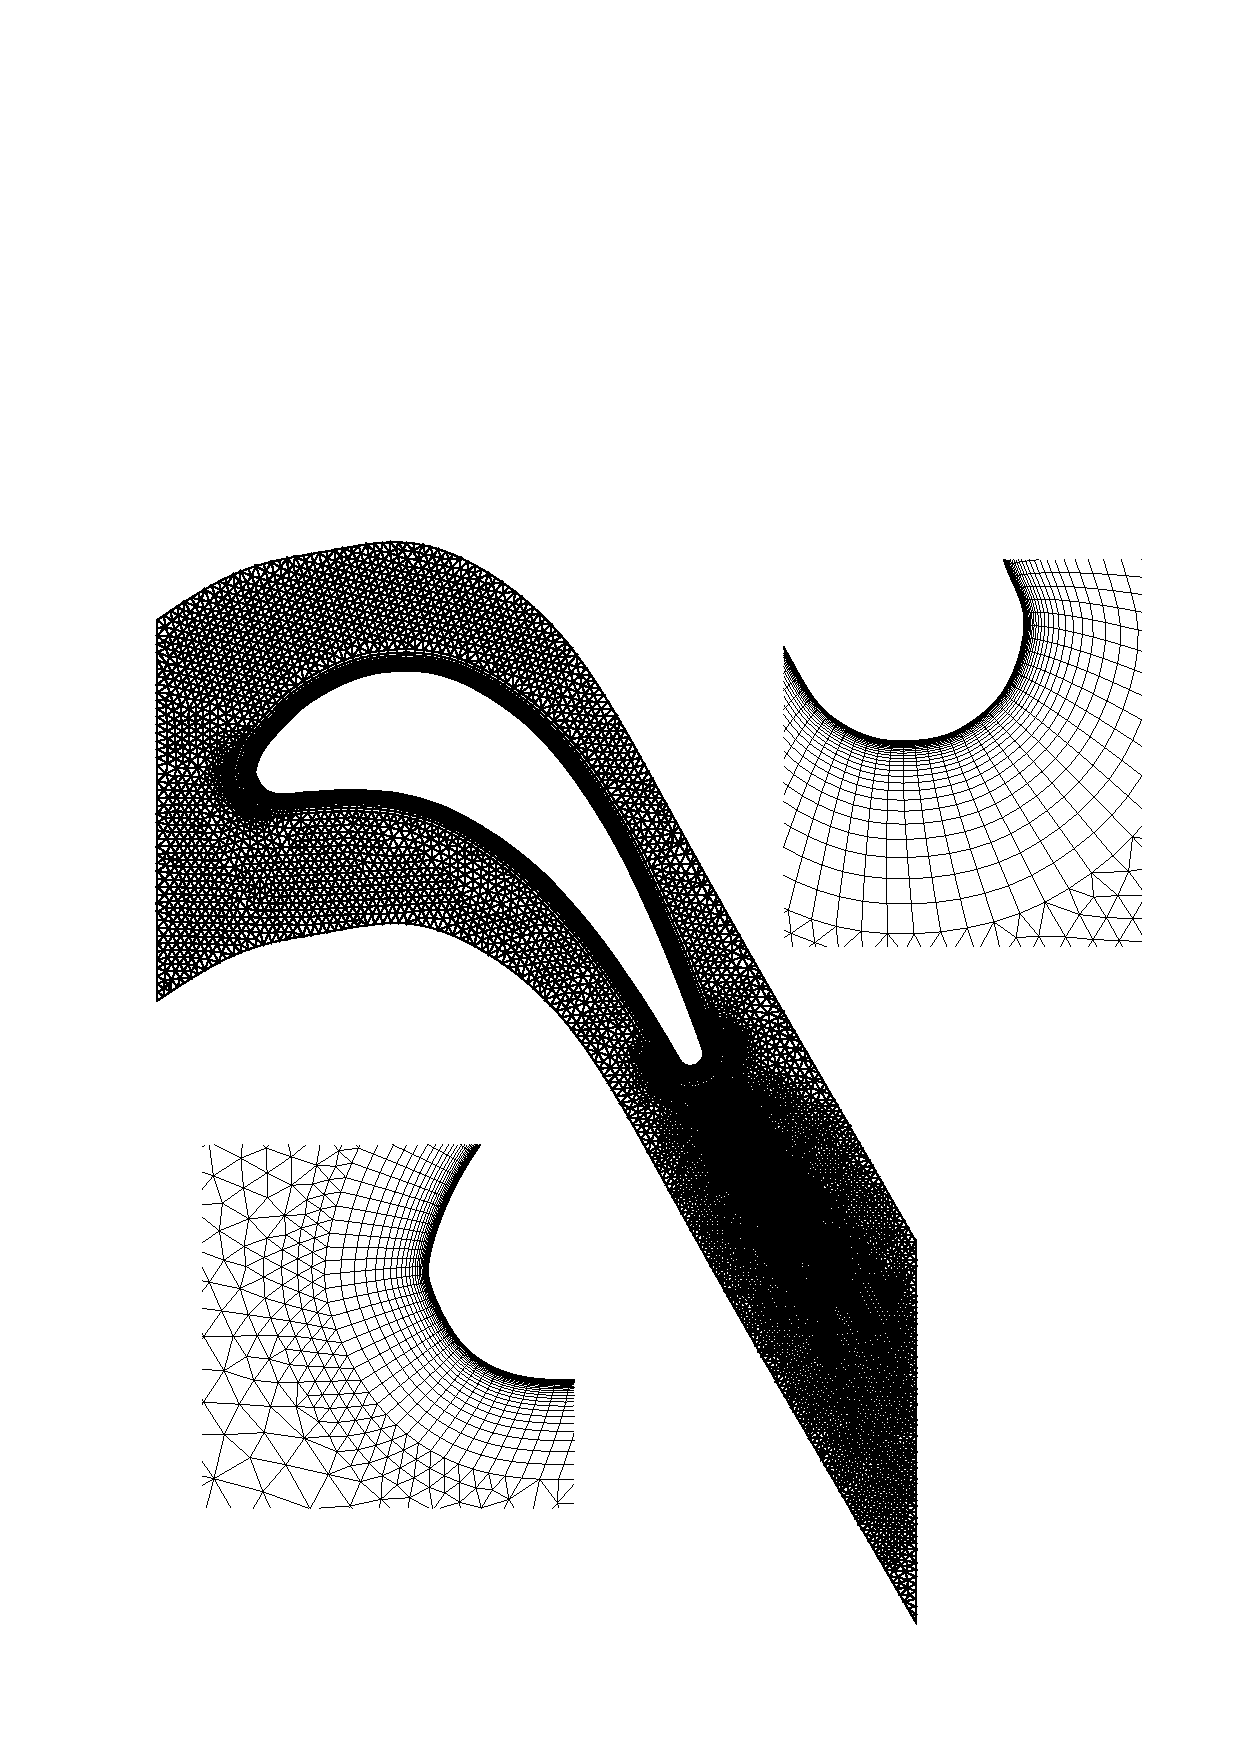
\includegraphics[width=110mm,clip=t]{CHAP_NONLIN/FIGURE/vki_mesh_1.pdf}}
 \caption{VKI LS59 rotor blade. Computational mesh with zoom views at leading- and
          trailing-edges}
 \label{vki_mesh_1.fig}
\end{figure}
%

 The inlet flow angle is $30\se{o}$ while the Reynolds number
 based on the blade chord and outlet conditions is in the range from
 $6.2\cdot10\se{5}$ up to $8.3\cdot10\se{5}$.
 A view of the computational mesh is shown in Fig. \ref{vki_mesh_1.fig}.
 This mesh contains 7,440 quadrilaterals in the boundary layer region and
 12,842 triangles in the rest of the domain which yields a total of 14,203 points.
%
%
\begin{figure}
 \begin{center}
  \begin{tabular}{ccc}
    \subfigure[Grid 2: 3587 cells]
       {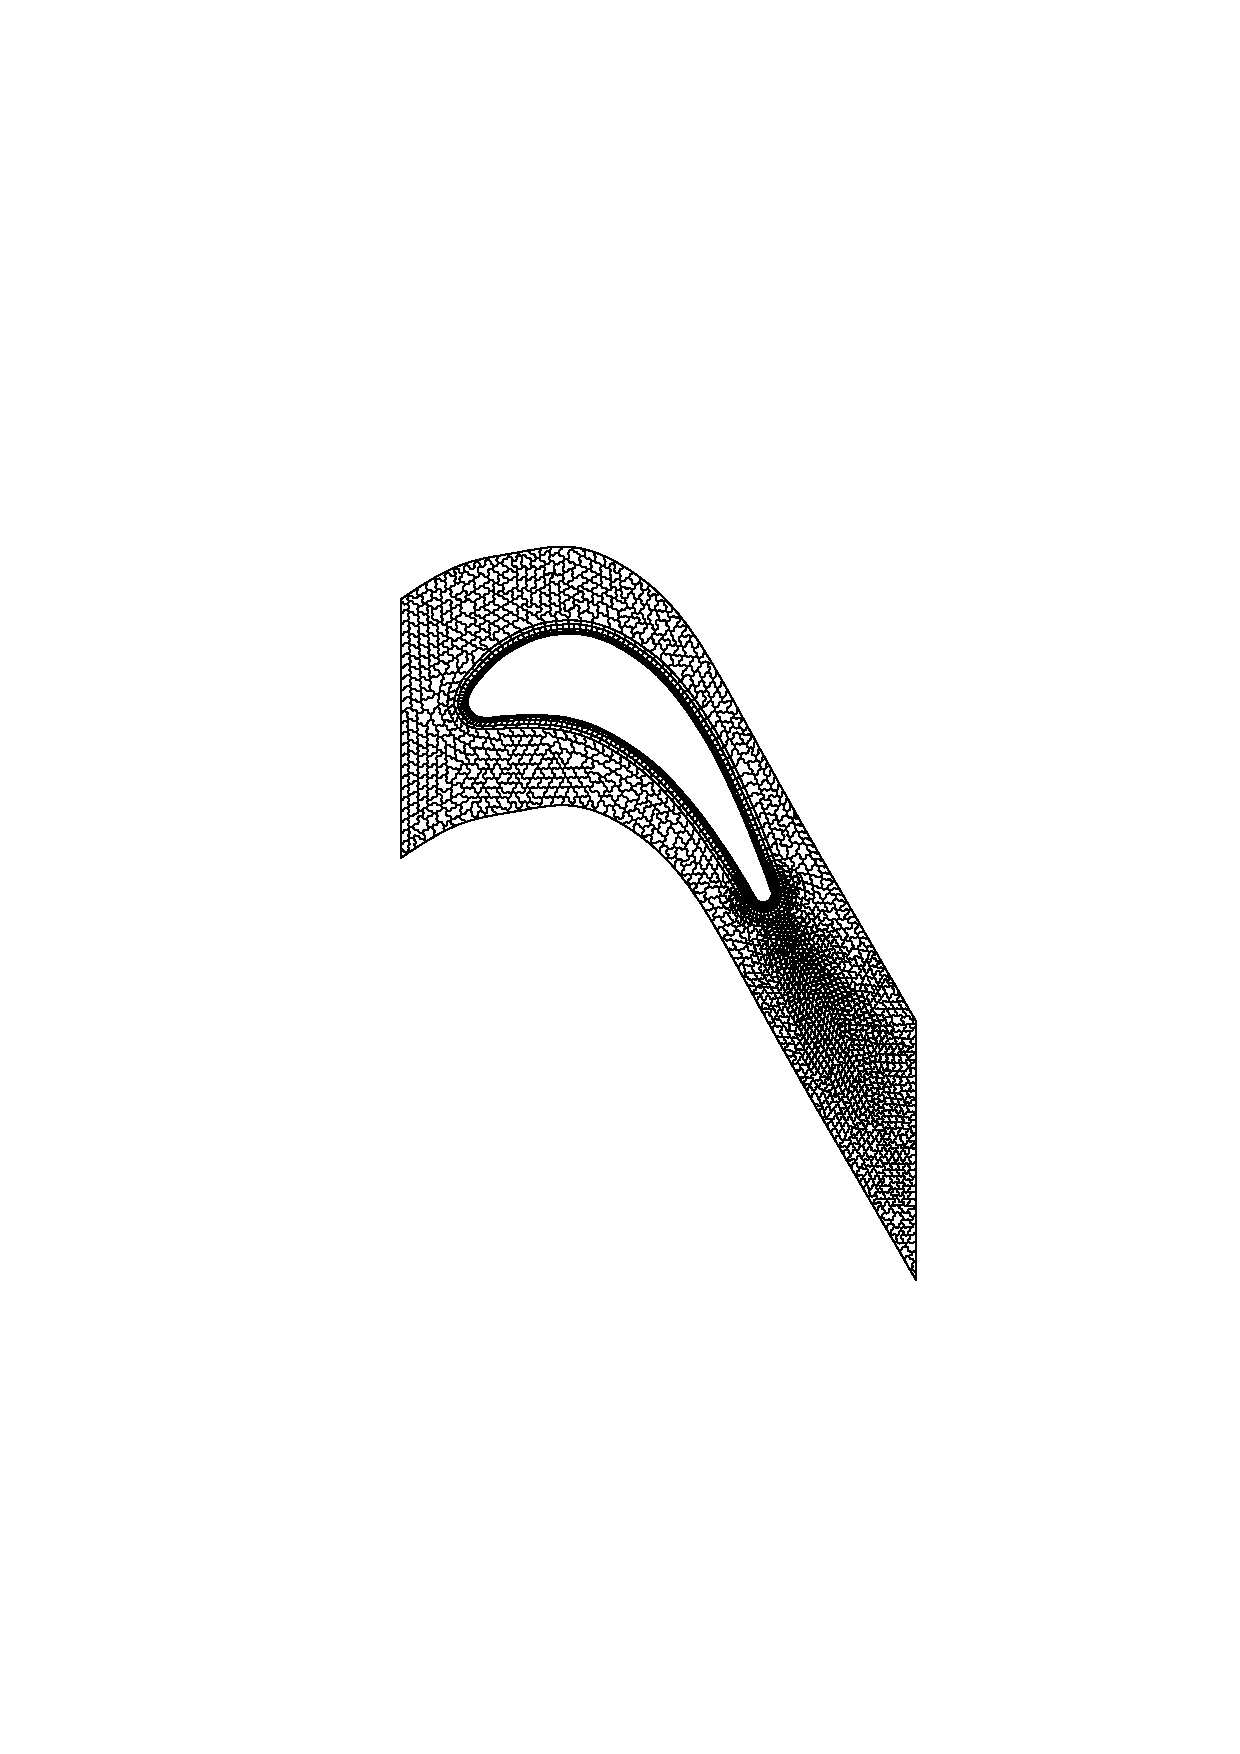
\includegraphics[width=45mm,clip=t]{CHAP_NONLIN/FIGURE/vki_mesh2.pdf}}
        &
    \subfigure[Grid 3: 908 cells]
       {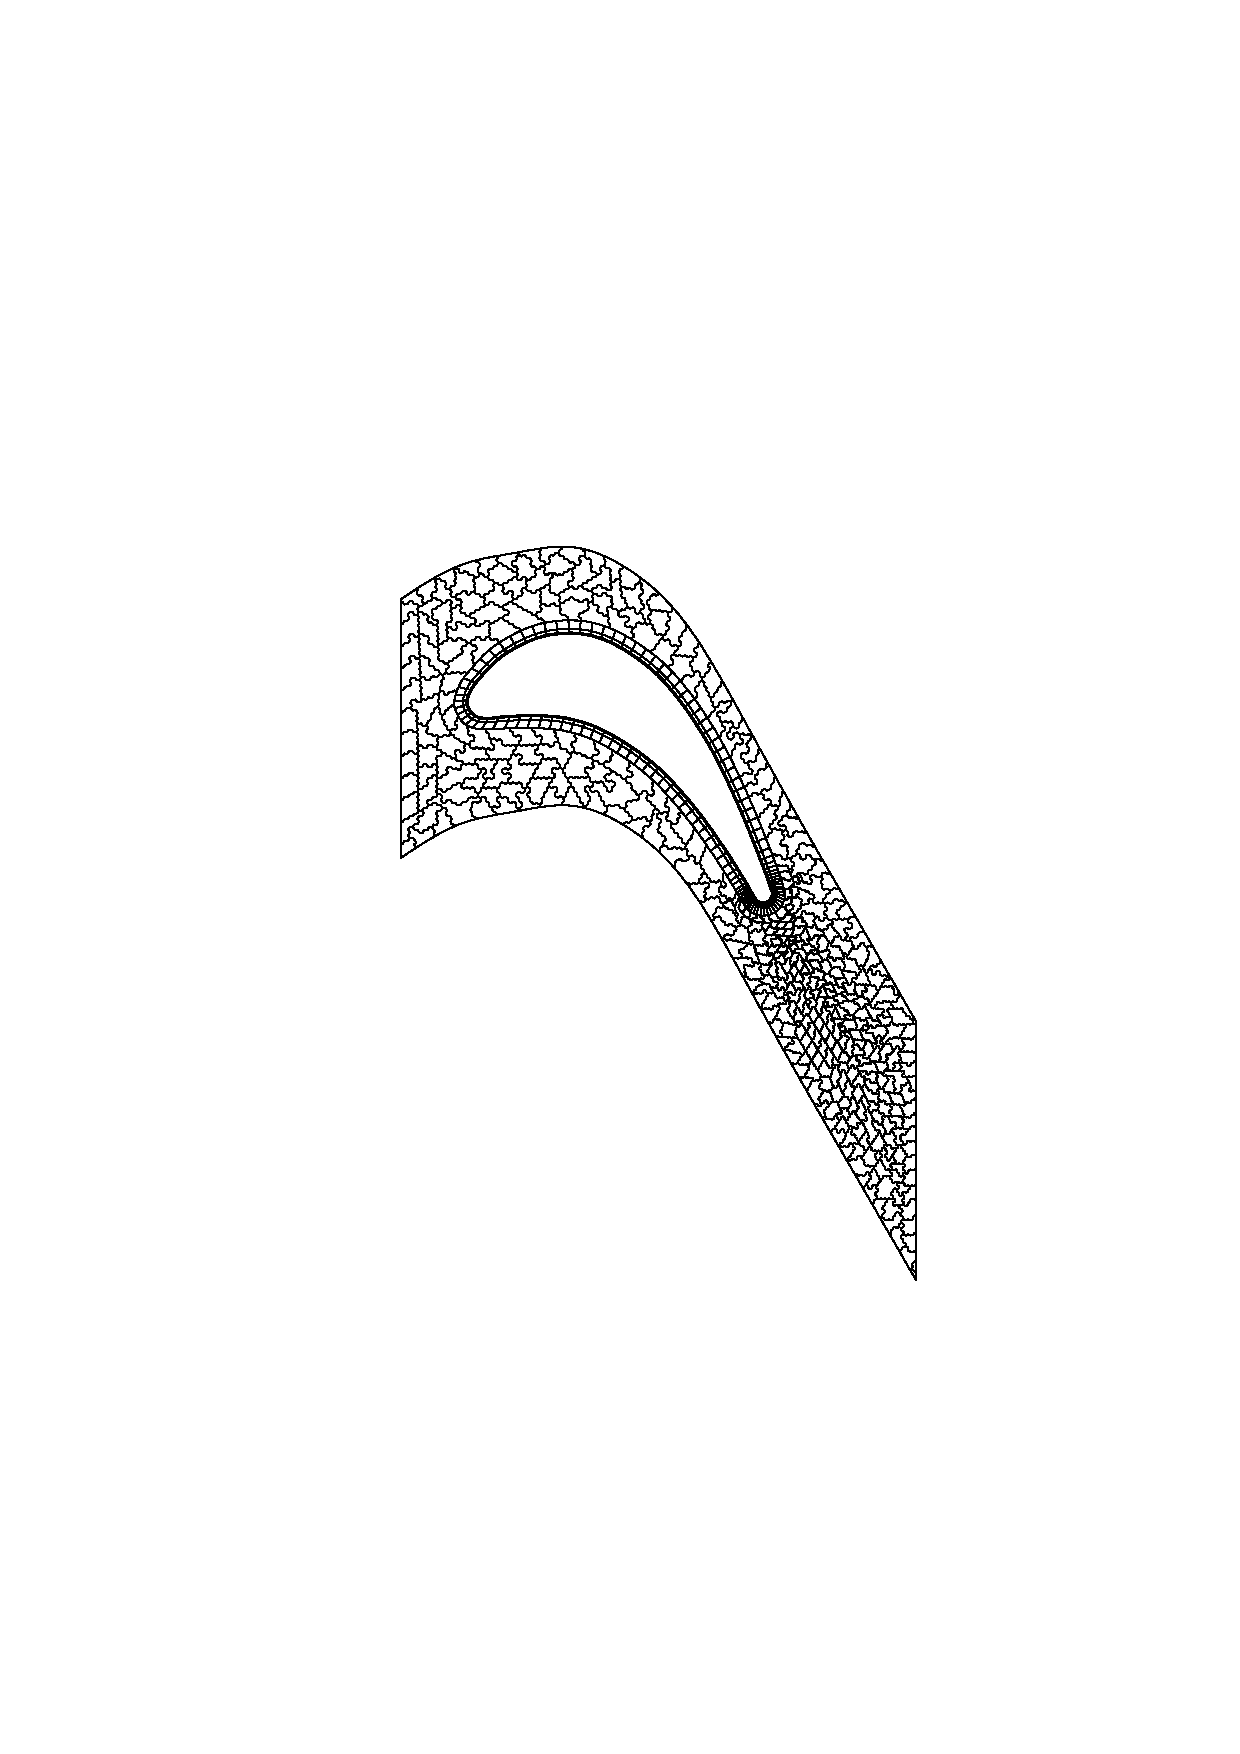
\includegraphics[width=45mm,clip=t]{CHAP_NONLIN/FIGURE/vki_mesh3.pdf}}
        &
    \subfigure[Grid 4: 239 cells]
       {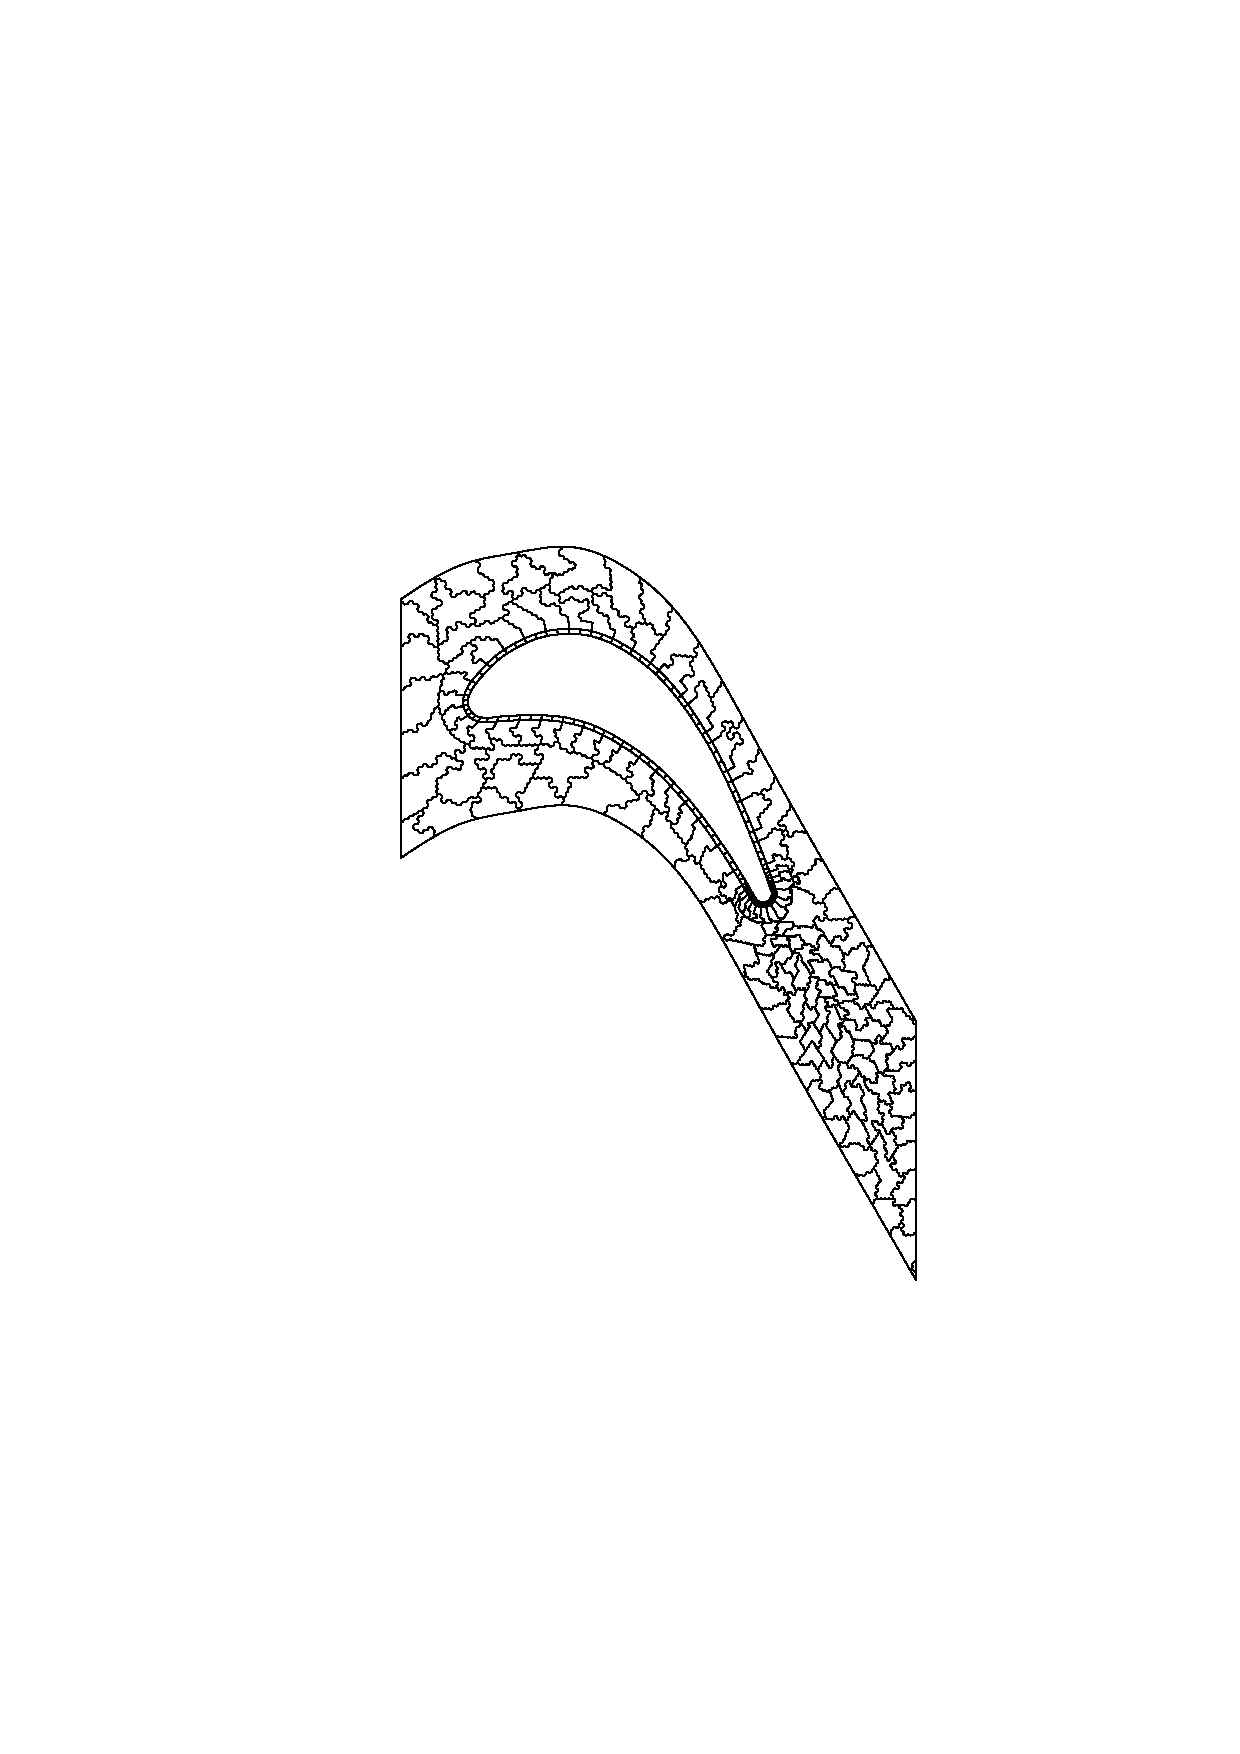
\includegraphics[width=45mm,clip=t]{CHAP_NONLIN/FIGURE/vki_mesh4.pdf}}
  \end{tabular}
 \end{center}
 \vspace{-5mm}
 \caption{VKI LS59 rotor blade. Agglomerated grids}
 \label{vki_agglo.fig}
\end{figure}
%
 Three succesively agglomerated meshes were used in a four grid W-type cycle
 in conjunction with the line-implicit preconditioner described
 in Appendix \ref{multigrid.chap}.
 Fig. \ref{vki_agglo.fig} shows the control volumes associated with
 these agglomerated grids.
%
\begin{figure}
  \centerline{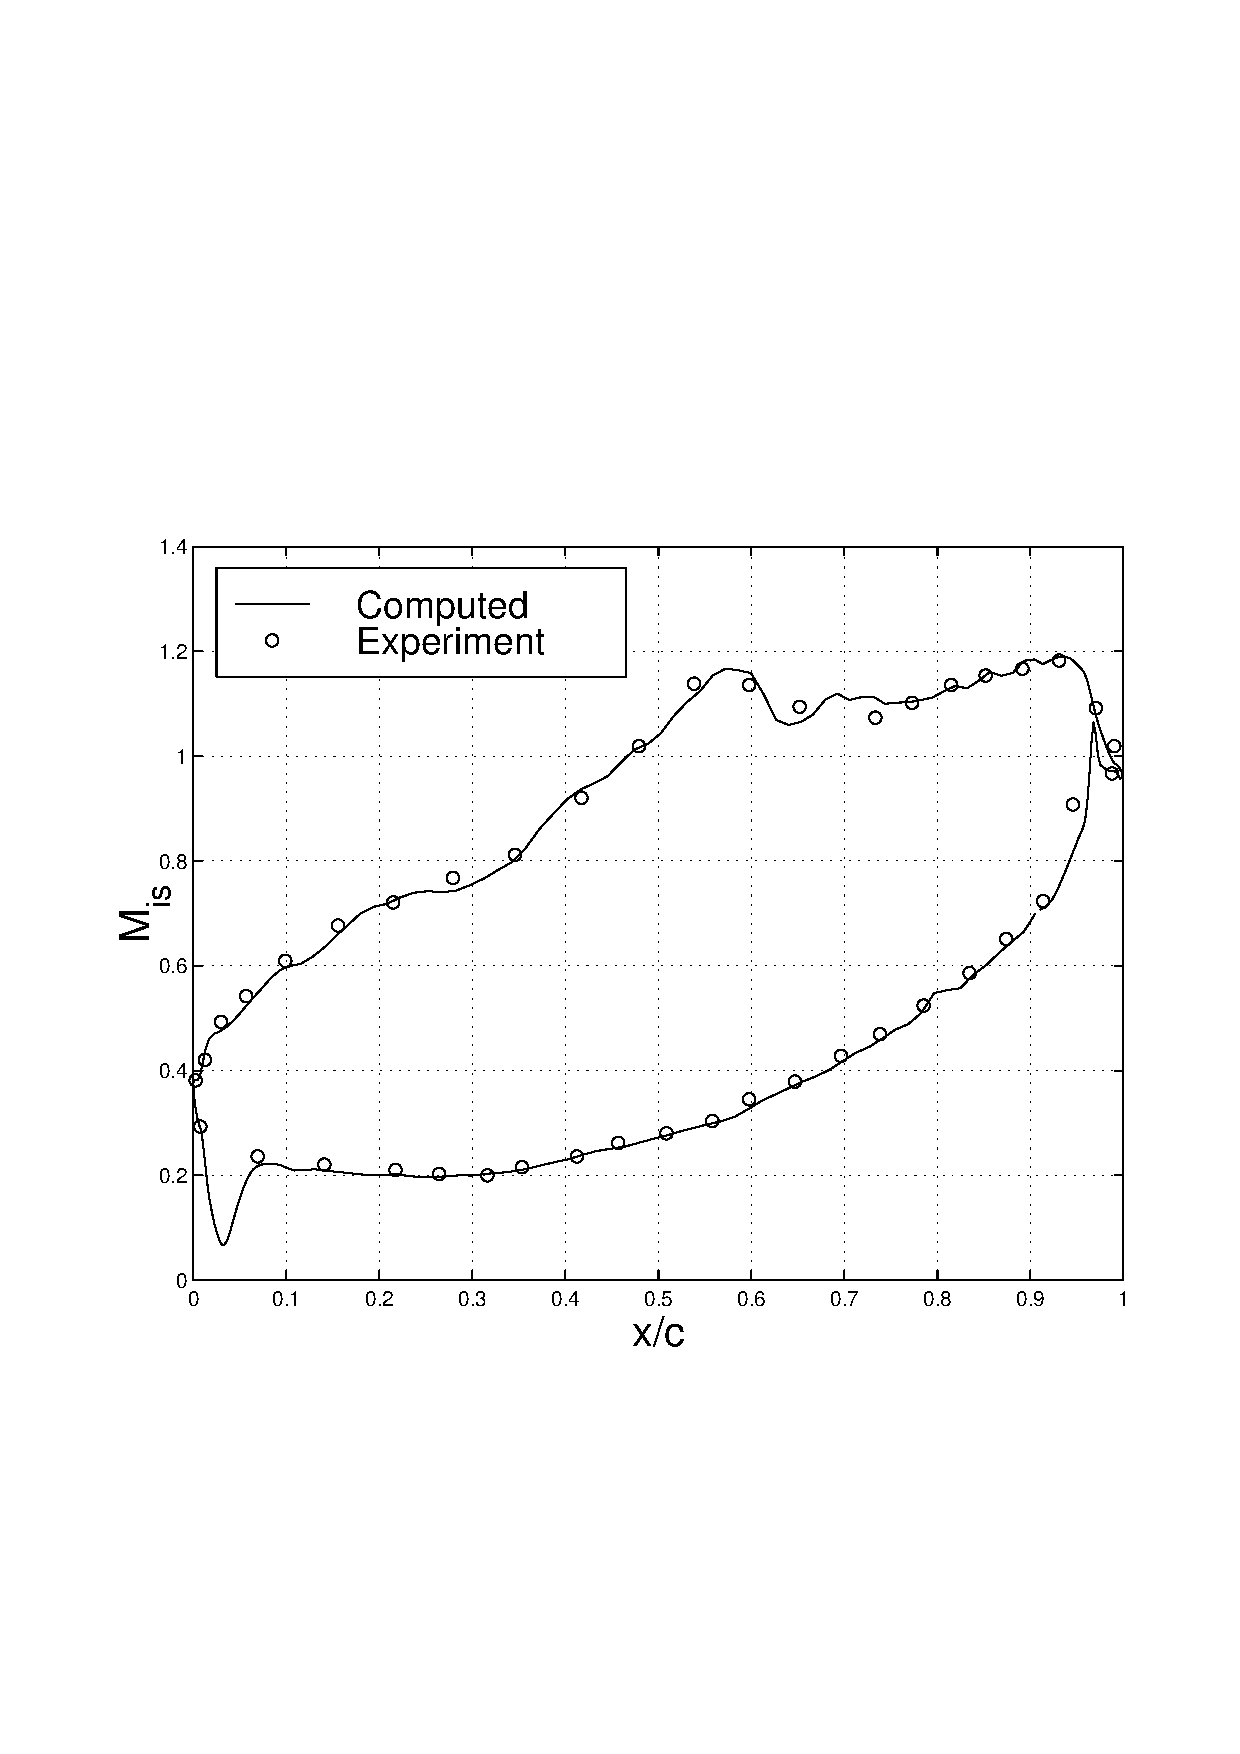
\includegraphics[width=130mm,clip=t]{CHAP_NONLIN/FIGURE/vki_blade.pdf}}
 \vspace{-5mm}
 \caption{VKI LS59 rotor blade. $M\sm{is2} = 1$, $Re\sm{2} = 7.6\cdot10\se{5}$.
          Isentropic Mach number distribution}
 \label{vki_mach_blade.fig}
\end{figure}
%
%
\begin{figure}
 \begin{center}
  \begin{tabular}{cc}
    \subfigure[Mach number contours]
       {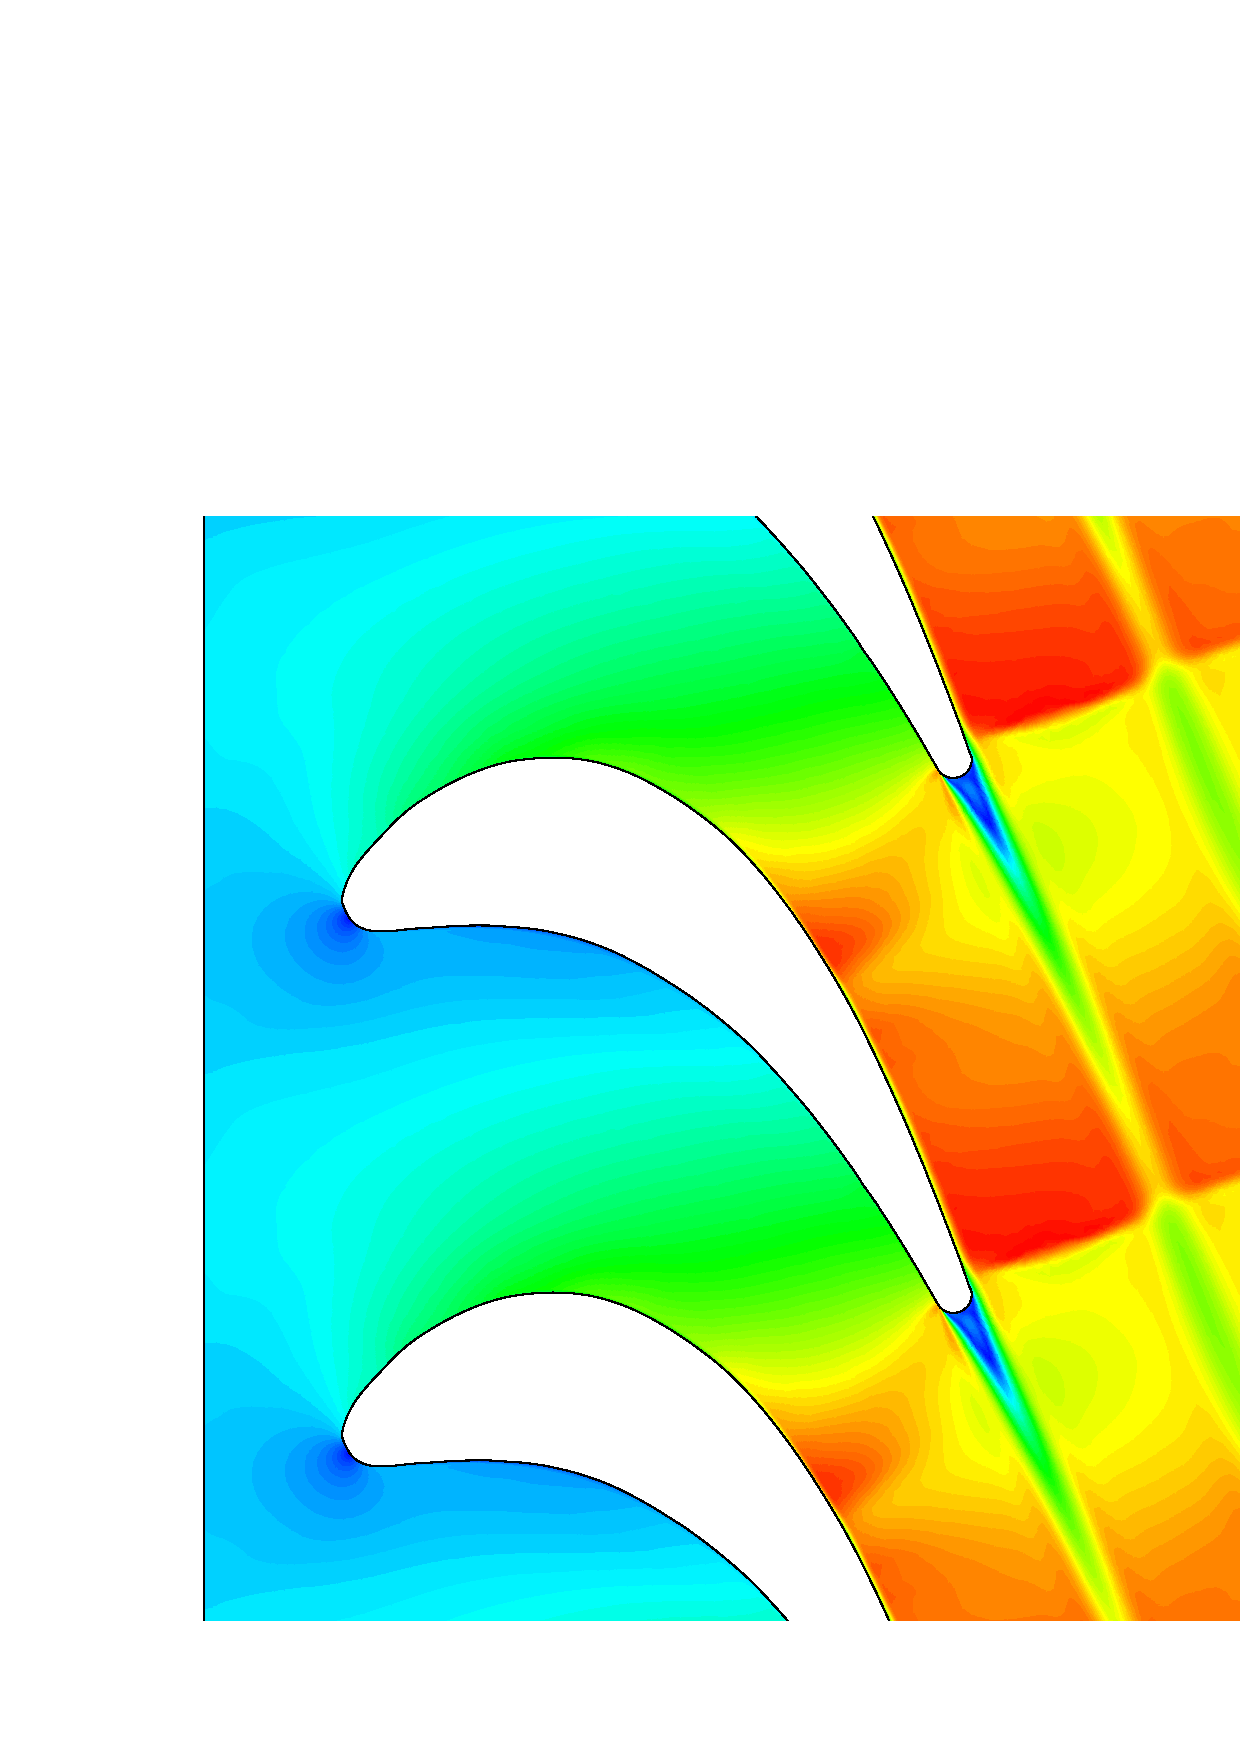
\includegraphics[width=70mm,clip=t]{CHAP_NONLIN/FIGURE/vki_mach.pdf}}
        &
    \subfigure[Particle traces near the trailing edge]
       {\fbox{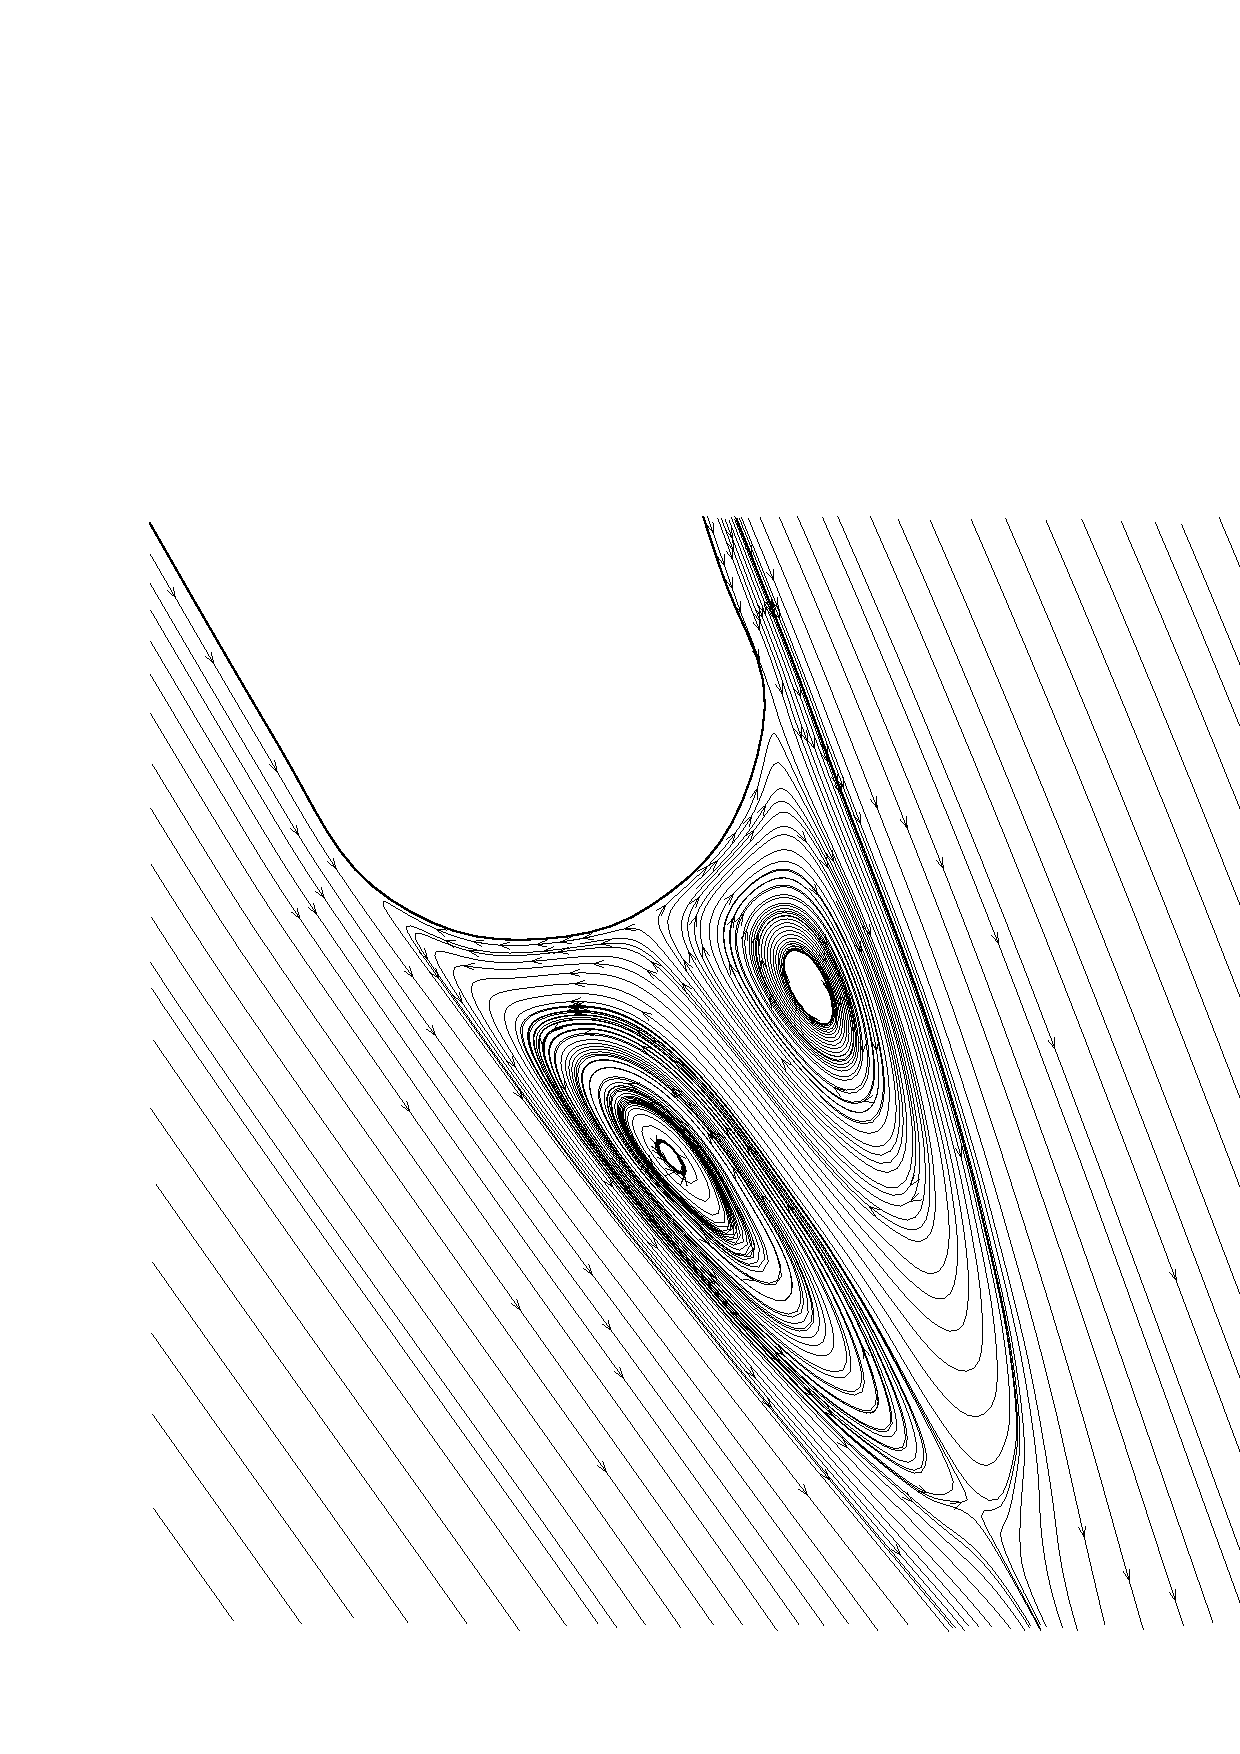
\includegraphics[width=70mm,clip=t]{CHAP_NONLIN/FIGURE/vki_traces.pdf}}}
  \end{tabular}
 \end{center}
 \vspace{-8mm}
 \caption{VKI LS59 rotor blade. $M\sm{is2} = 1$, $Re\sm{2} = 7.6\cdot10\se{5}$.
          Computed solution}
 \label{vki_mach.fig}
\end{figure}
%

 The isentropic Mach number distribution on the blade surface is given in
 Fig. \ref{vki_mach_blade.fig} for the case with an isentropic outlet Mach
 of unity. The sonic conditions are obtained at $x/c \approx 0.47$
 on the suction side and at the trailing edge in the pressure side
 resulting in fairly straight sonic line across the blade passage as
 shown in the Mach number contours of Fig. \ref{vki_mach.fig}a.
 The flow is accelerated along the suction side up to $x/c = 0.6$ followed
 by a moderate deceleration downstream.
 For this blade, the experimental data of
 Kiock et al. \citeyear{Kiock:1} include exit flow angles, inlet Mach number
 and loss coefficient defined as
 $\xi = 1 - \frac{\left|v\sm{2}\right|}{\left|v\sm{is2}\right|}$, where
 $v\sm{is2}$ represents the isentropic outlet velocity. The comparison
 between the experimental and the computed values of such quantities as a
 function of the outlet Mach number is reported in Fig. \ref{vki_blade.fig}.
%
%
\begin{figure}
 \begin{center}
  \begin{tabular}{c}
    \subfigure[Exit flow angle]
       {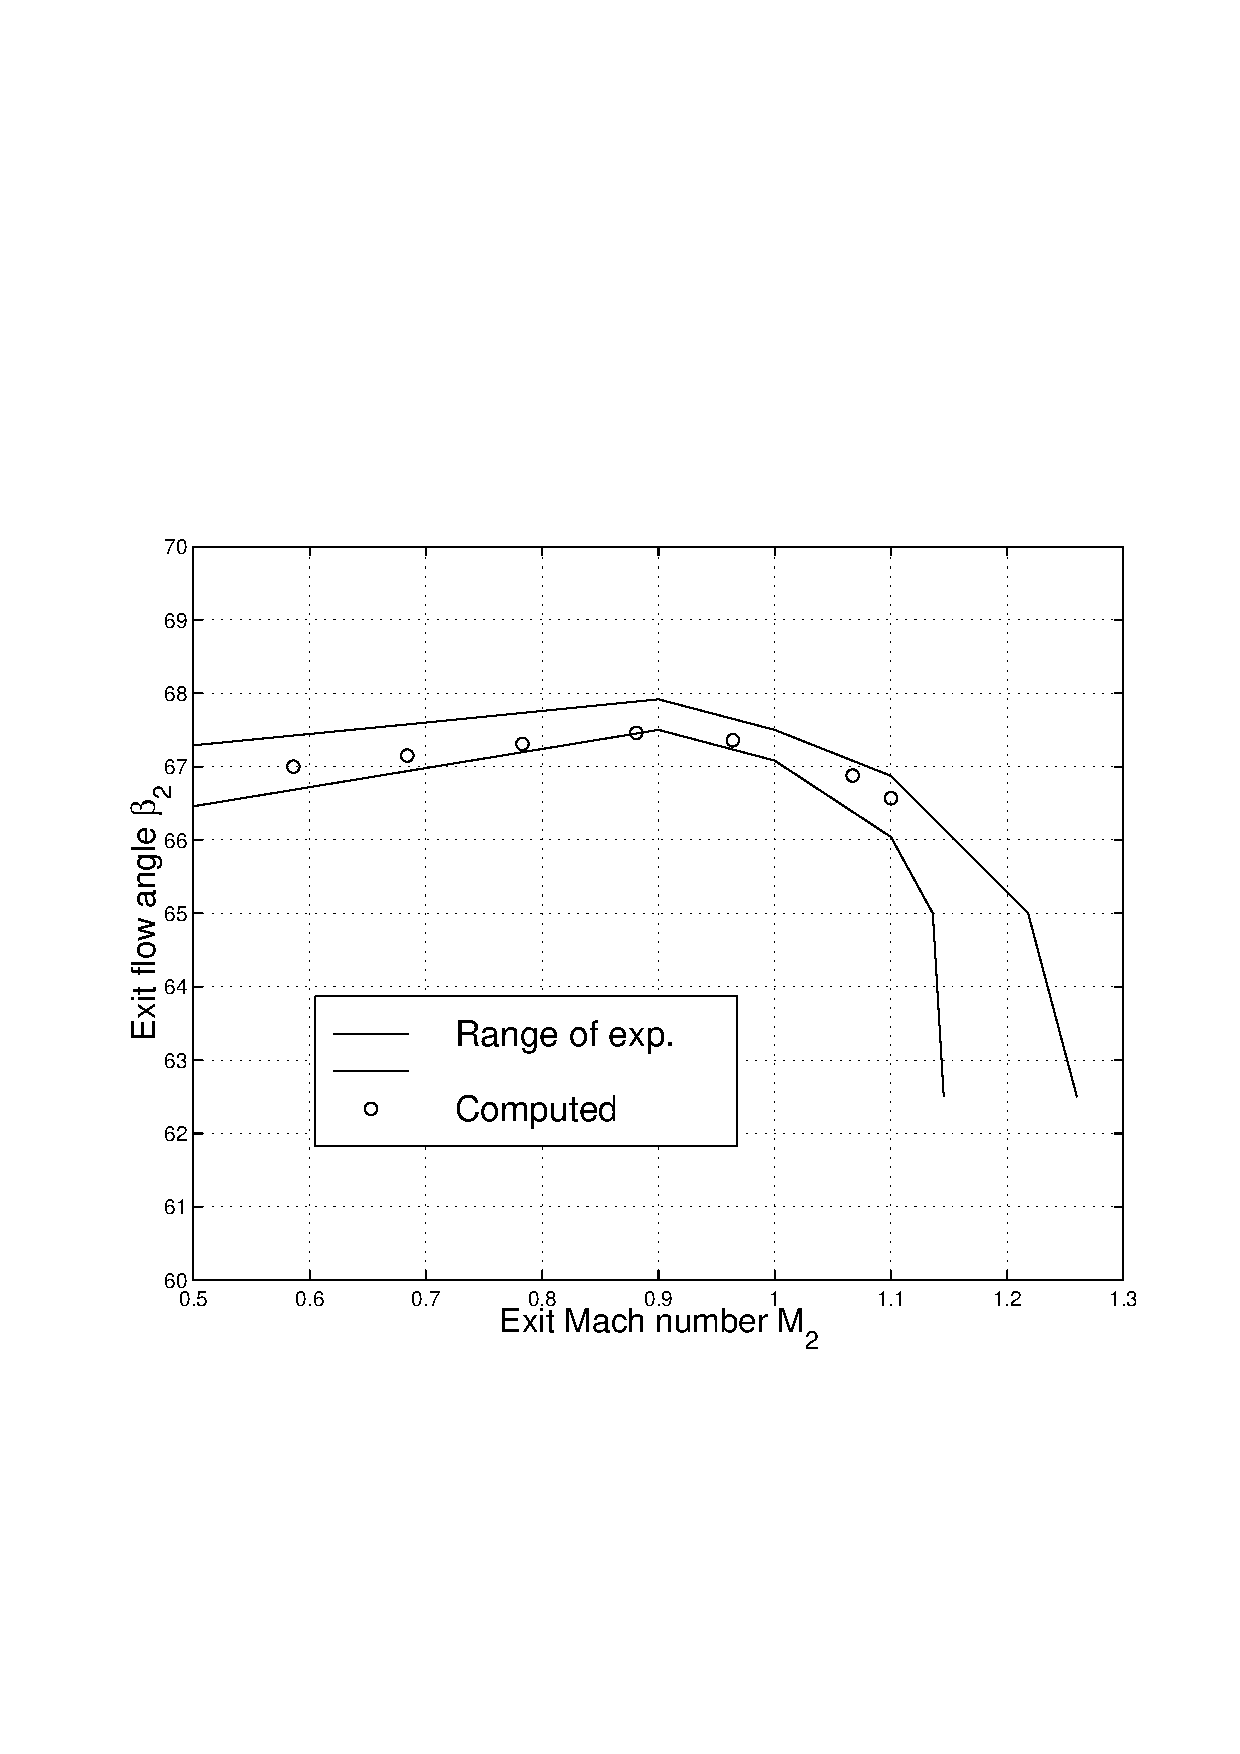
\includegraphics[width=80mm,clip=t]{CHAP_NONLIN/FIGURE/vki_beta2.pdf}}
        \vspace{-4mm}\\
    \subfigure[Inlet Mach number]
       {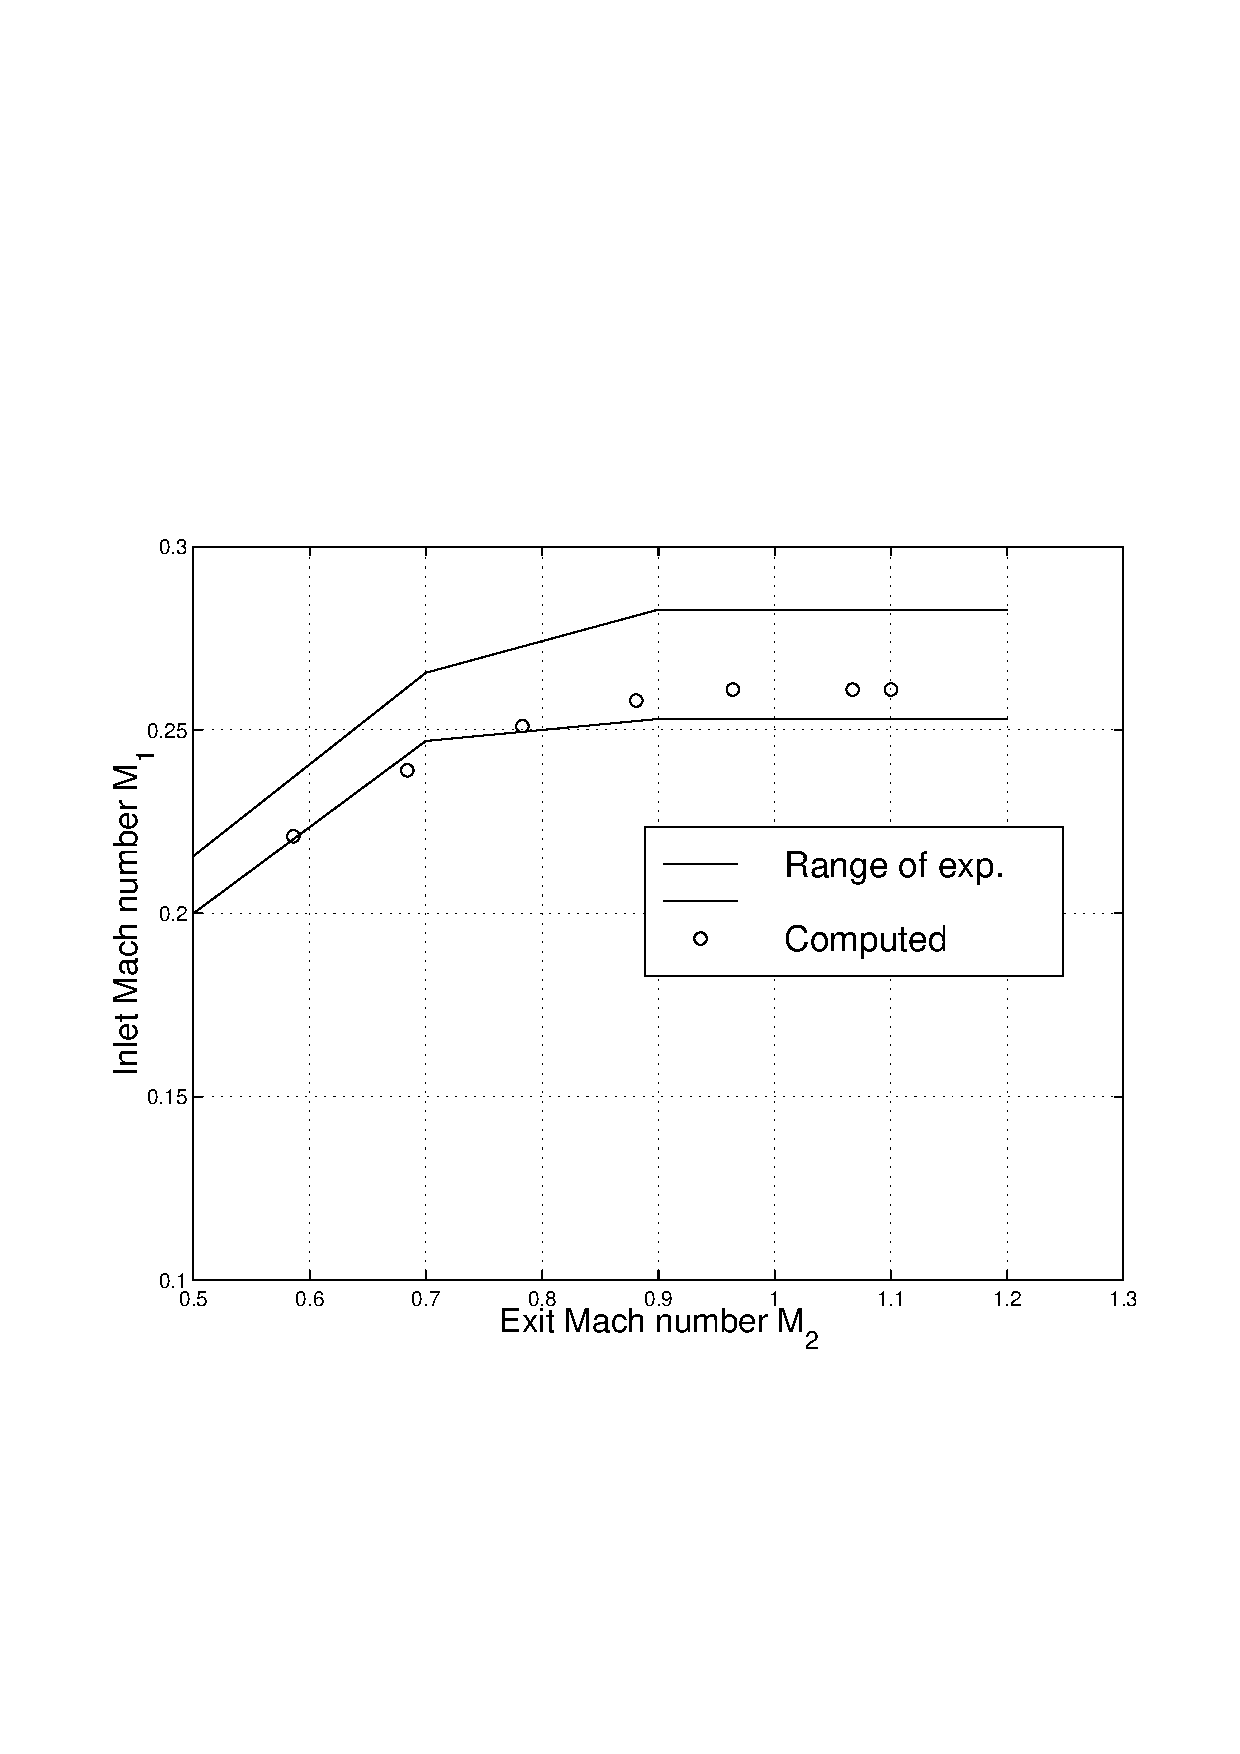
\includegraphics[width=80mm,clip=t]{CHAP_NONLIN/FIGURE/vki_mach1.pdf}}
        \vspace{-4mm}\\
    \subfigure[Loss coefficient]
       {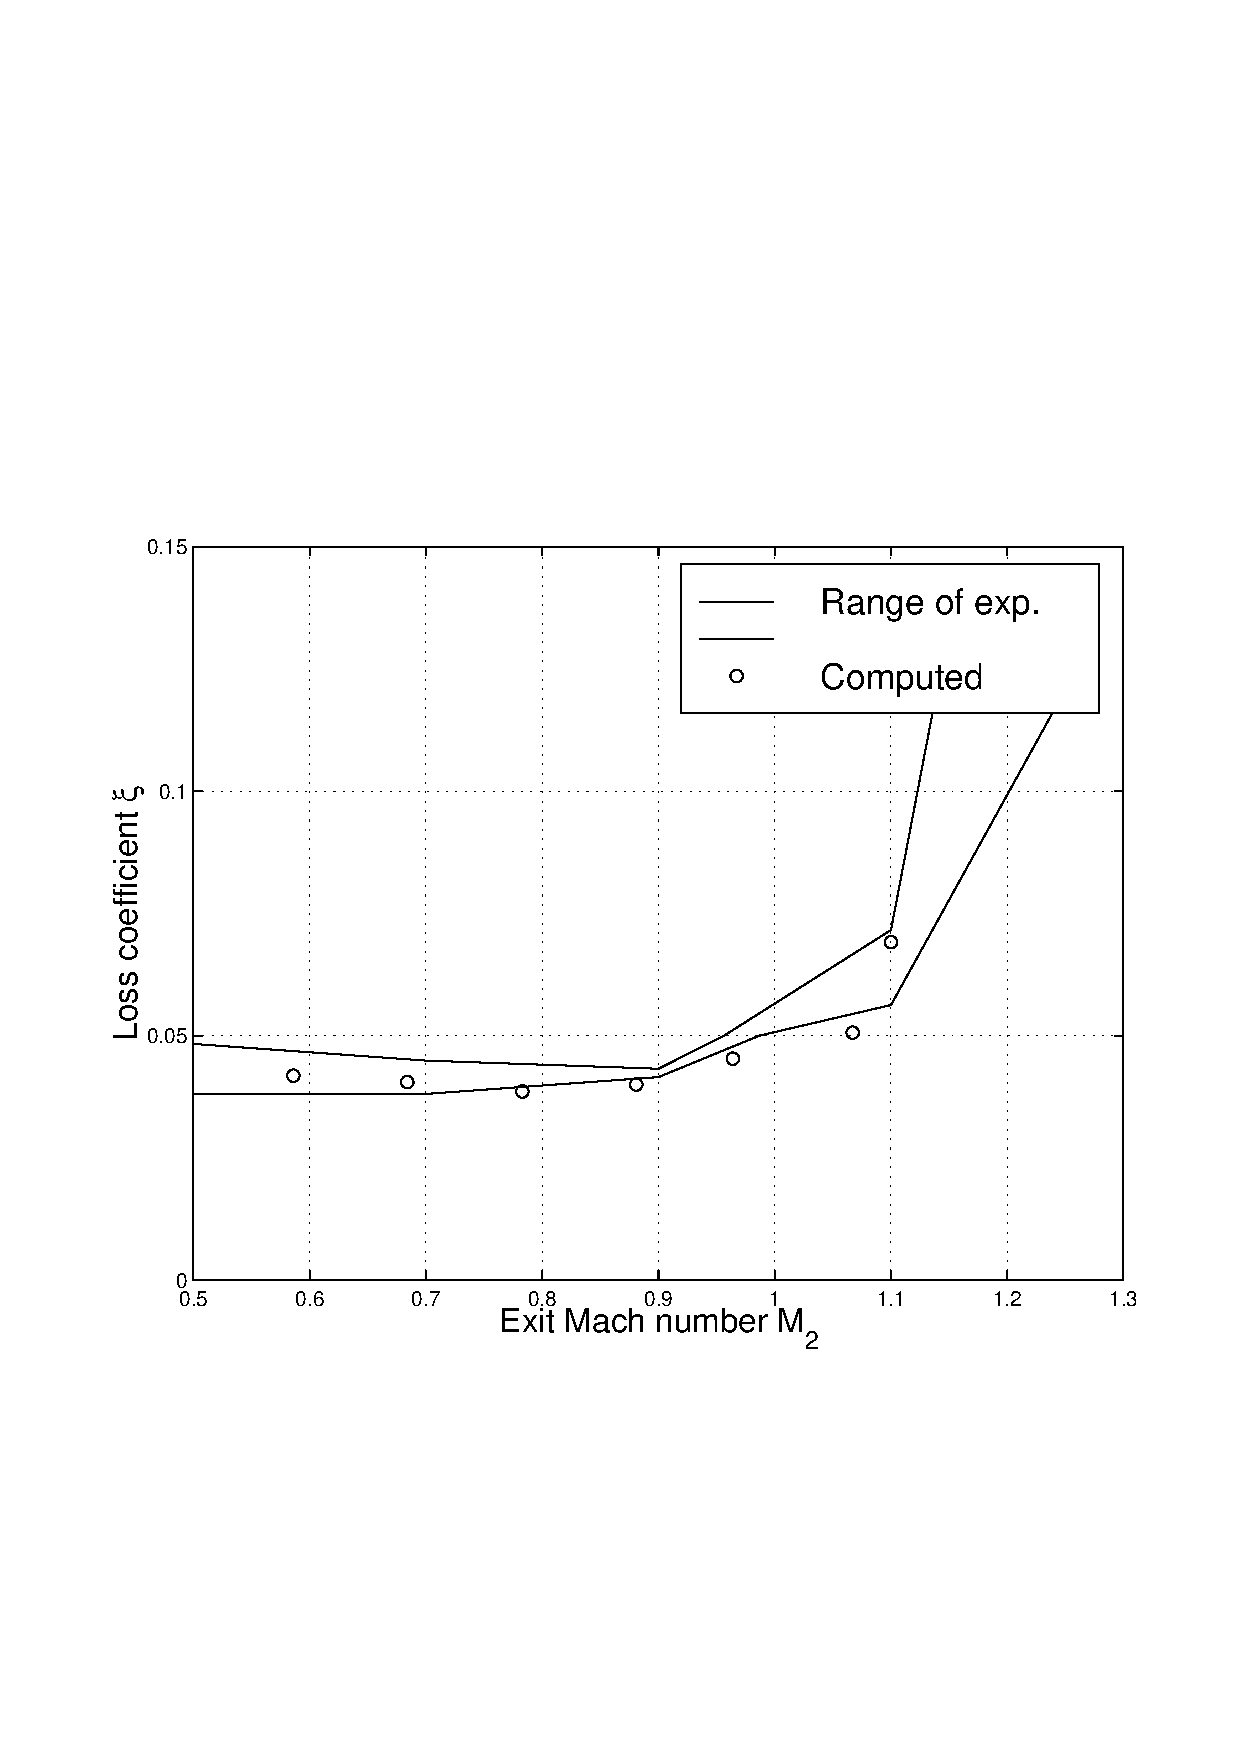
\includegraphics[width=80mm,clip=t]{CHAP_NONLIN/FIGURE/vki_loss.pdf}}
  \end{tabular}
 \end{center}
 \vspace{-8mm}
 \caption{VKI LS59 rotor blade. Computed solutions}
 \label{vki_blade.fig}
\end{figure}
%
%

 Fig. \ref{vki_res.fig} compares the convergence history obtained using the
 line-implicit solver of Appendix \ref{multigrid.chap}, on a single grid and
 on four grid W-type cycle. The convergence history
 of a single grid, point-Jacobi, iterative implicit scheme as the one
 used by Sayma et al. \citeyear{Luca:10}, is also plotted.
 It is evident that the single grid solution is not converged
 and the reason of this could be blamed to the grid anisotropy as well as
 to the blunt trailing edge of the blade which causes a recirculation bubble
 which could be inherently unsteady (Fig. \ref{vki_mach.fig}b).
 The single grid implicit scheme of Sayma et al. \citeyear{Luca:1} converges very slowly
 because not designed to be effective in damping error arising from highly stretched
 meshes.
%
\begin{figure}
 \centerline{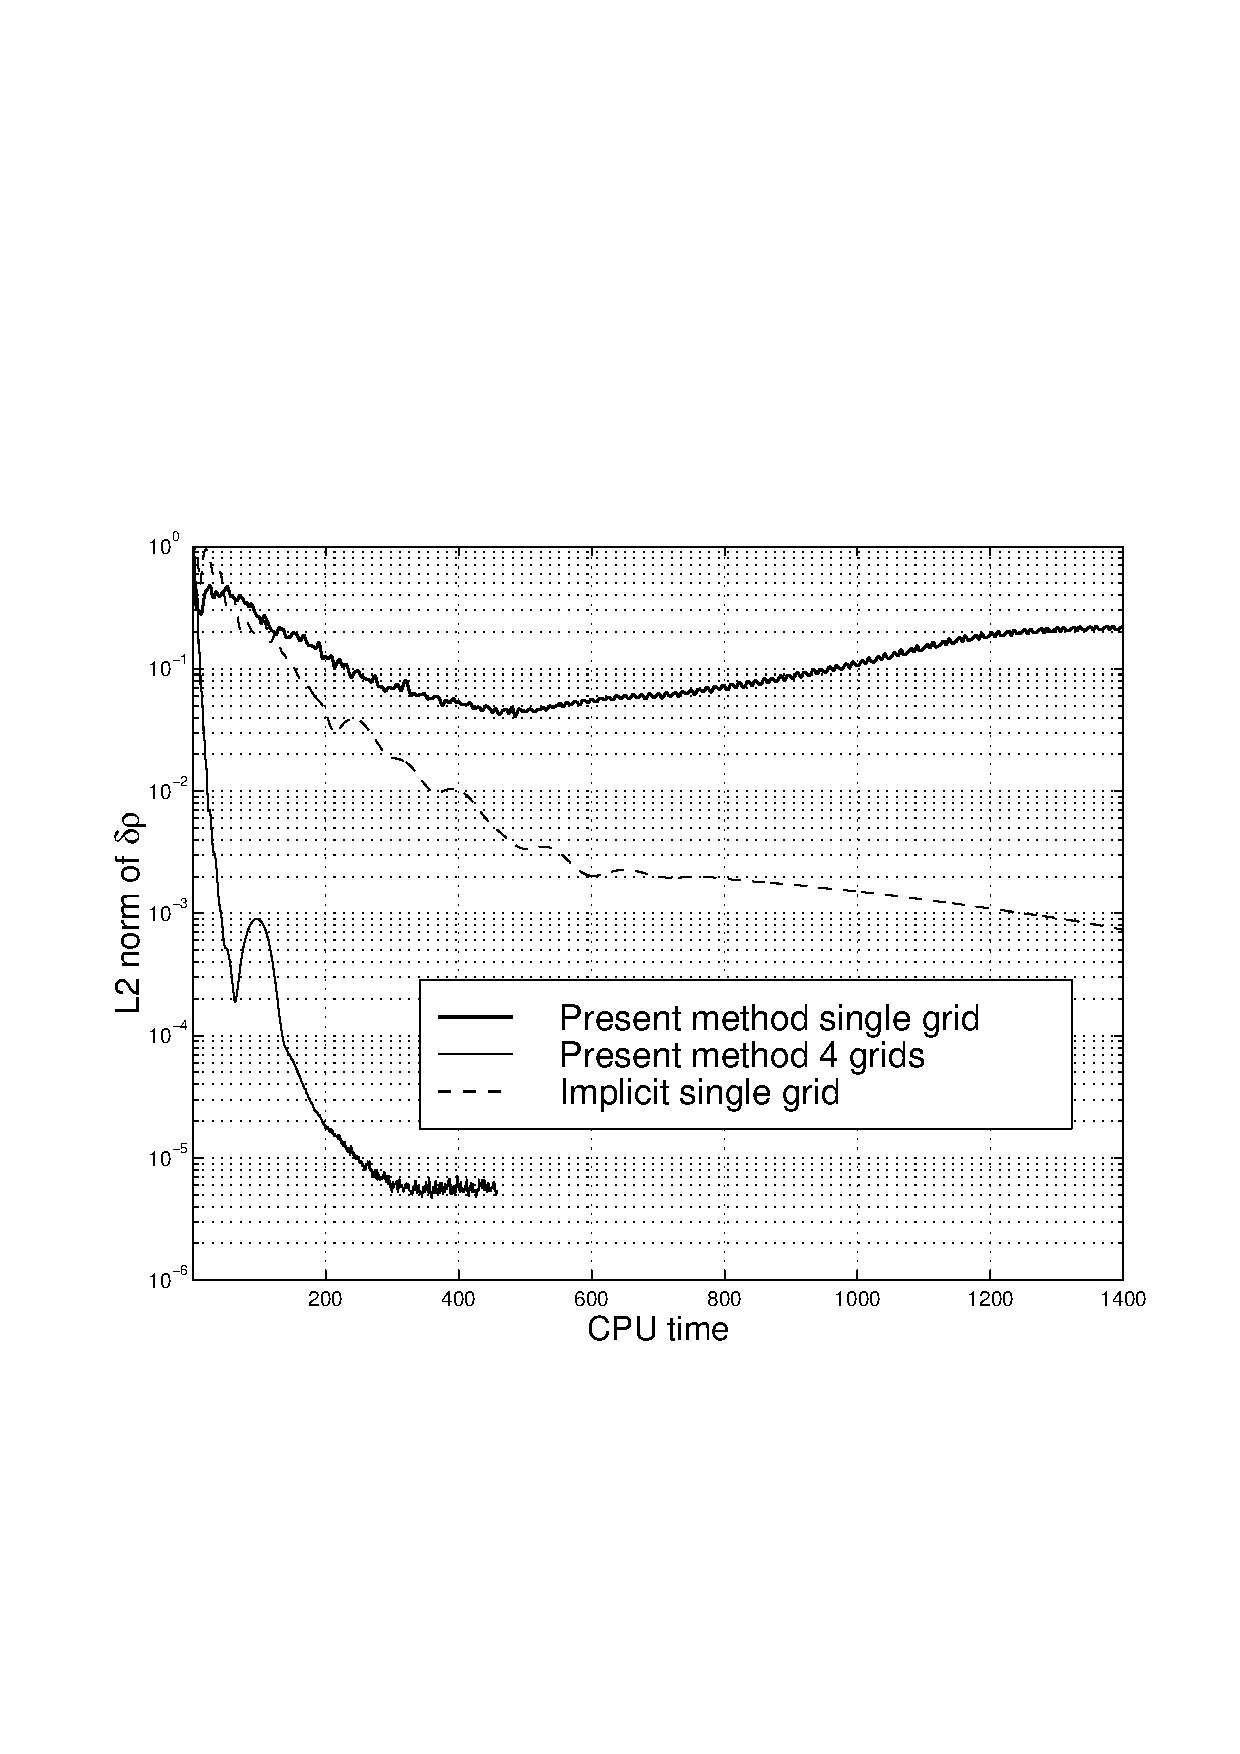
\includegraphics[width=130mm,clip=t]{CHAP_NONLIN/FIGURE/vki_res.pdf}}
 \caption{VKI LS59 rotor blade. Residual history}
 \label{vki_res.fig}
\end{figure}
%

%
%%
%
\subsection{NASA Rotor 37}
\label{nasa_rotor37.subsec}
%
 A low-aspect-ratio transonic inlet rotor for a core compressor,
 designated NASA rotor 37, was used in the present section to validate
 the steady state code for three-dimensional geometries.
 The rotor was originally designed and tested at NASA Lewis Research
 Center by Reid and Moore \citeyear{Reid:1}.
 In the CFD assessment, the rotor was tested in isolation by several
 researchers (Suder and Celestina \citeyearNP{Suder:1},
 Chima \citeyearNP{Chima:2}, Arima et al. \citeyearNP{Arima:1}).
 The rotor geometry together with the location measured using
 aerodynamics probes and laser anemometer measurements
 are shown in Fig. \ref{rot37_geo.fig}.
%
\begin{figure}
  \begin{center}
   \begin{tabular}{c}
    \subfigure
      {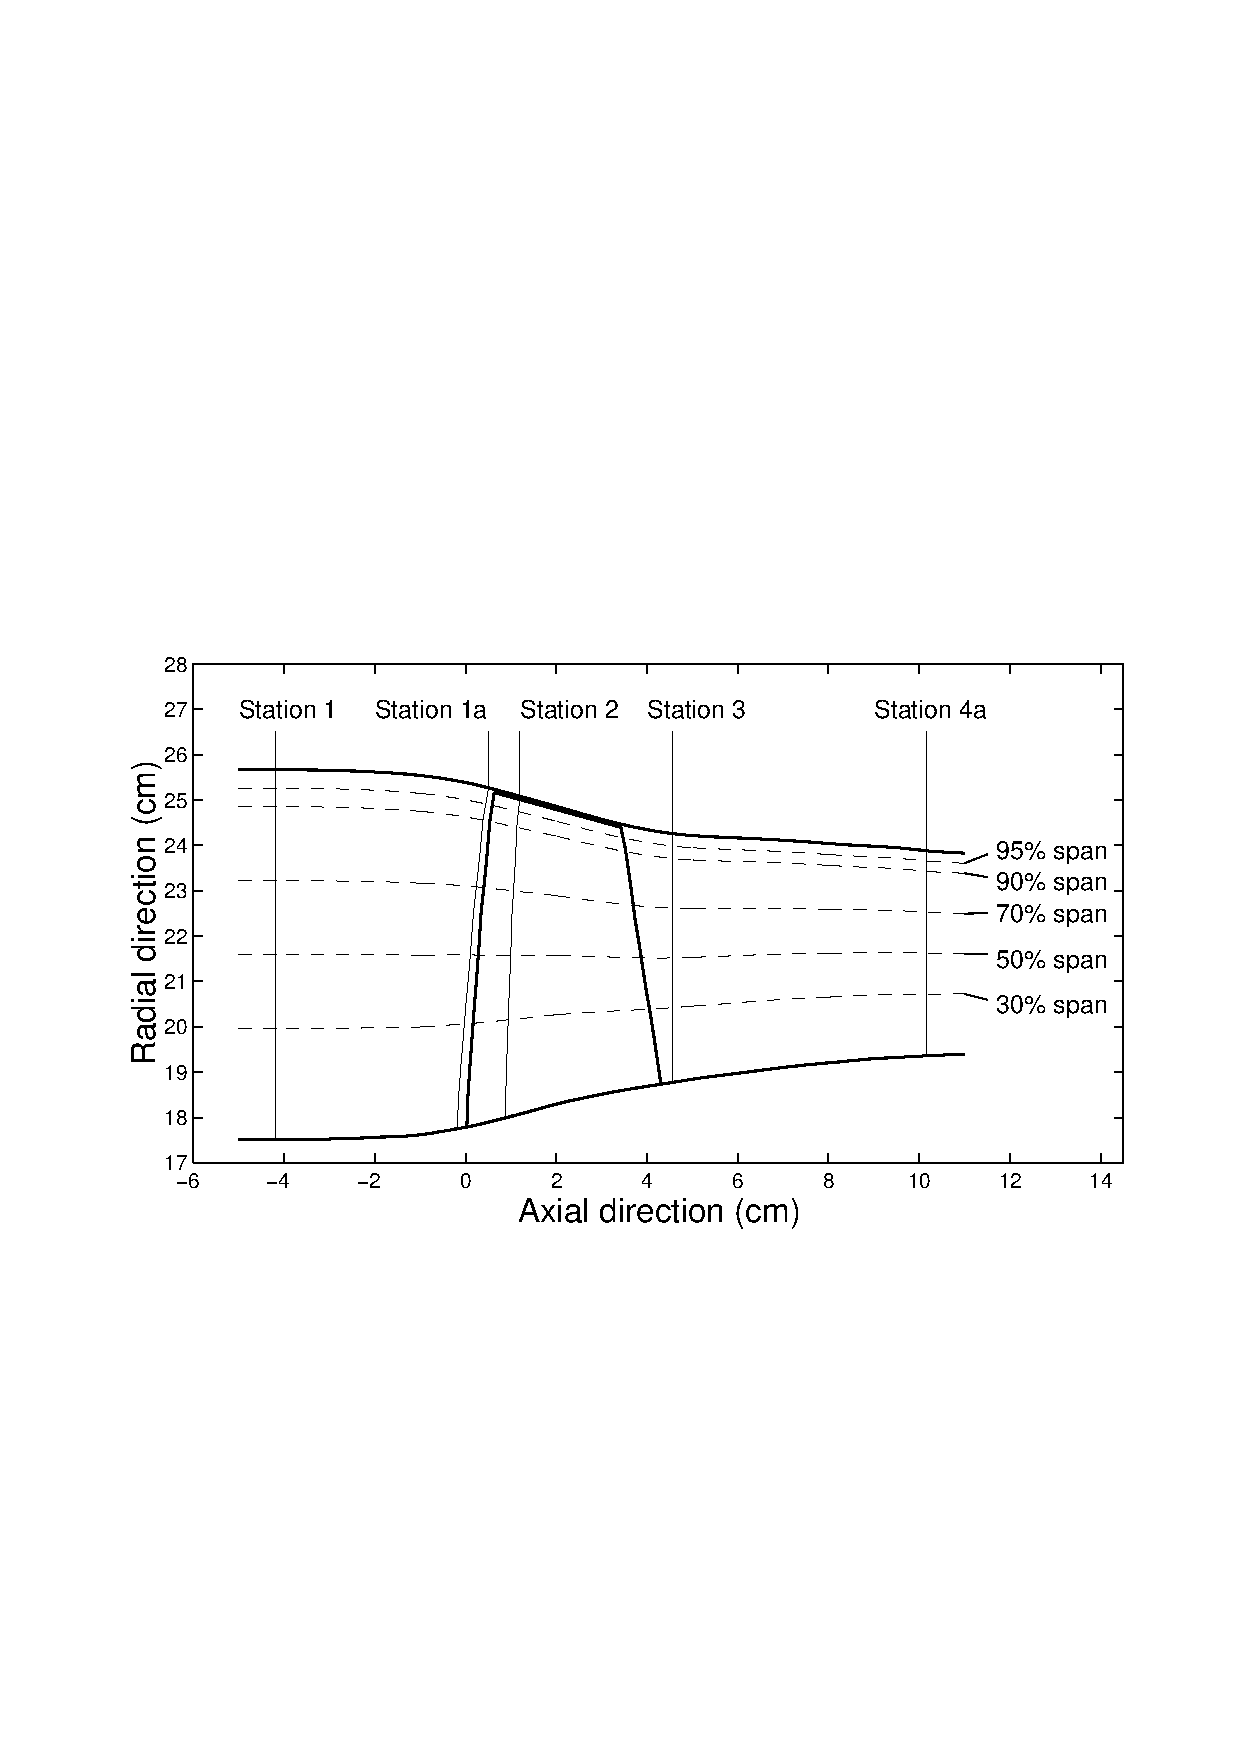
\includegraphics[width=100mm,clip=t]{CHAP_NONLIN/FIGURE/rotgeo.pdf}}
      \vspace{-4mm}\\
    \subfigure
      {\begin{tabular}{|c|c|c|c|c|c|}\hline
        Station & 1 & 1a & 2 & 3 & 4a \\ \hline
        x (cm) & -4.19 & $-5\%$ chord & $20\%$ chord & 4.57 & 10.16 \\ \hline
      \end{tabular}}
   \end{tabular}
  \end{center}
  \vspace{-8mm}
  \caption{NASA Rotor 37: $x-r$ view showing locations at which data were
           acquired}
  \label{rot37_geo.fig}
\end{figure}
%

 The rotor has a design pressure ratio of 2.106 at a mass flow of
 $20.19\ kg/s$, with a measured chocking mass flow of $20.93\ kg/s$.
 The rotor has 36 multiple-circular-arc blades with a hub-tip ratio
 of 0.7, an aspect ratio of 1.19, and a tip solidity
 of 1.288. The running tip clearance was estimated to be $0.356\ mm$
 ($0.45\%$ span). The design wheel speed is $17,188.7\ rpm$
 giving a nominal tip speed of $454\ m/s$.
 A brief description of the test facility and laser anemometer
 system is given by Suder and Celestina \citeyear{Suder:1}.

%
\begin{figure}
 \begin{center}
  \begin{tabular}{cc}
    \subfigure[Frontal view]
       {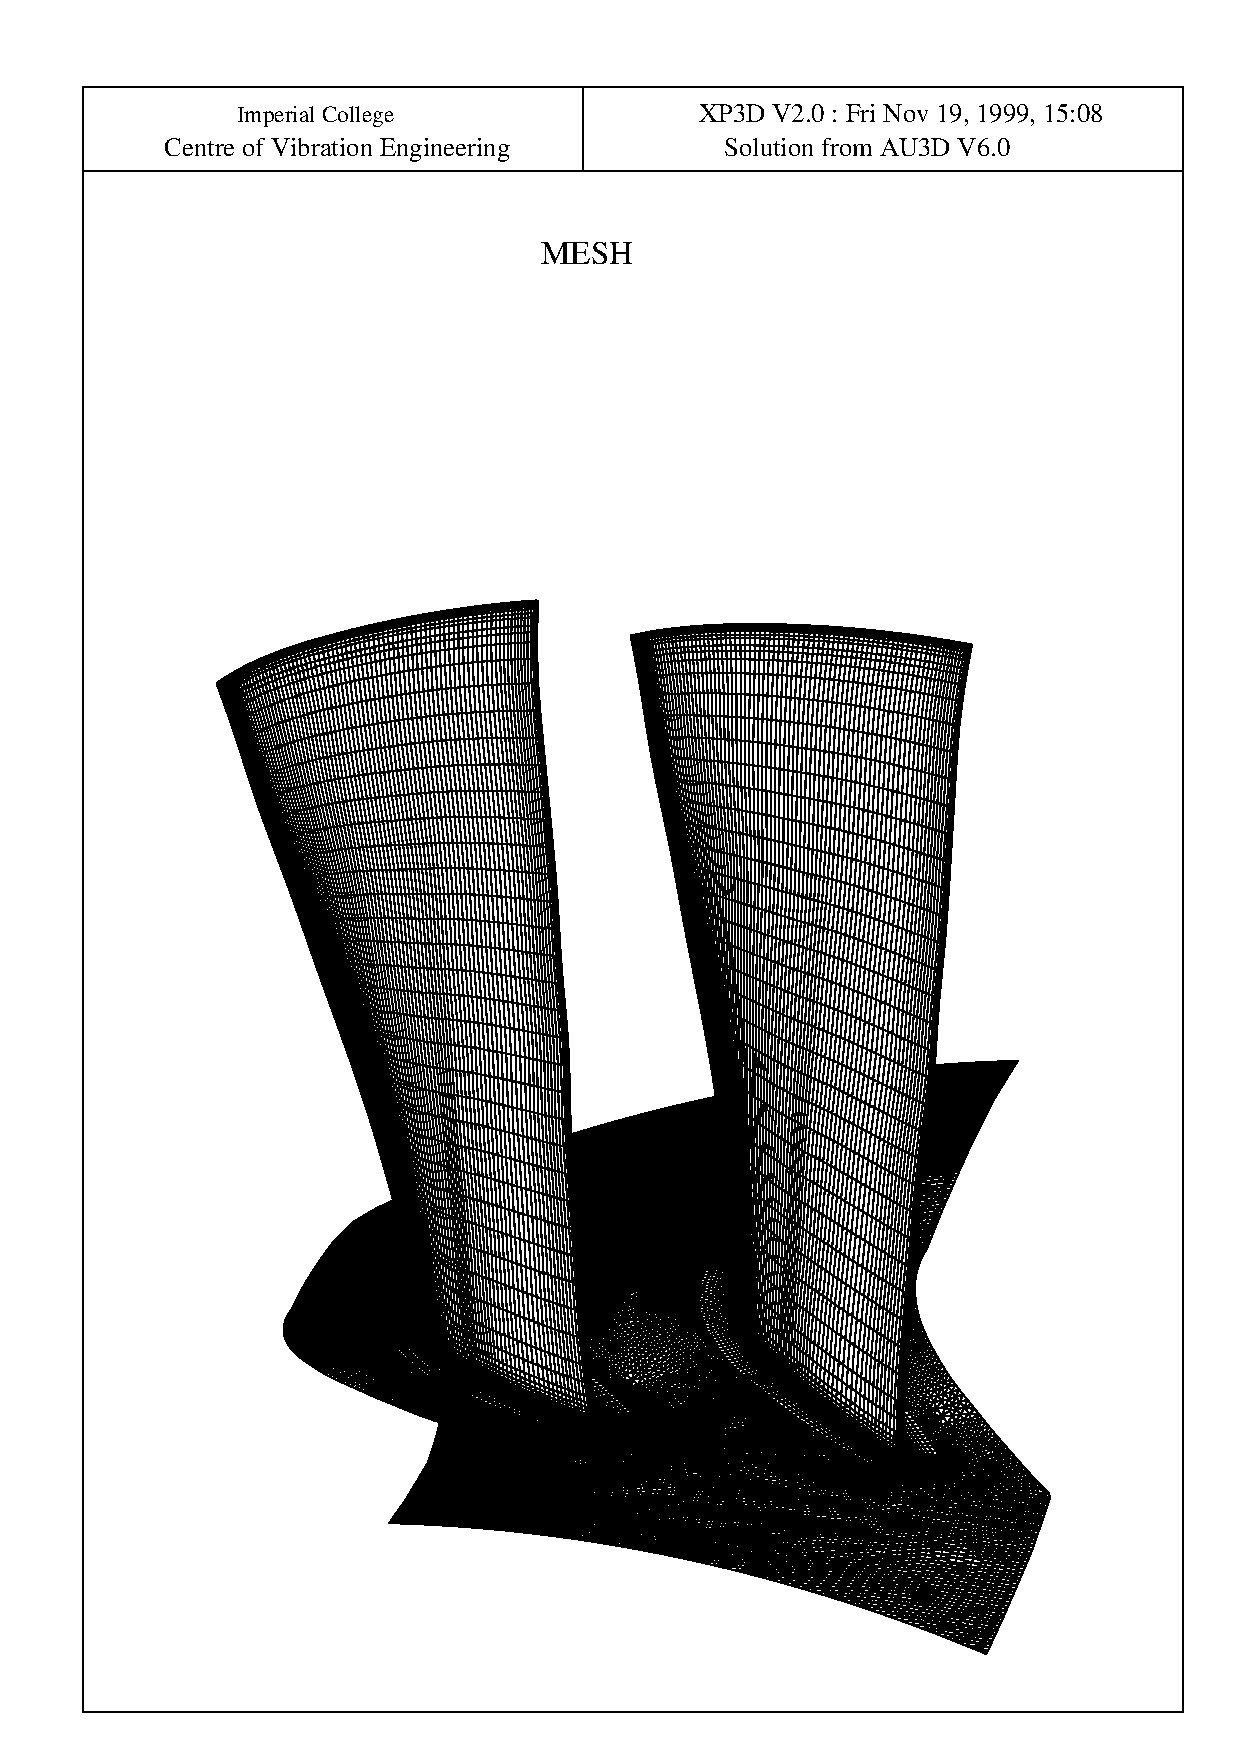
\includegraphics[width=55mm,clip=t]{CHAP_NONLIN/FIGURE/rot37_mesh1.pdf}}
        &
    \subfigure[$x-r\theta$ view]
       {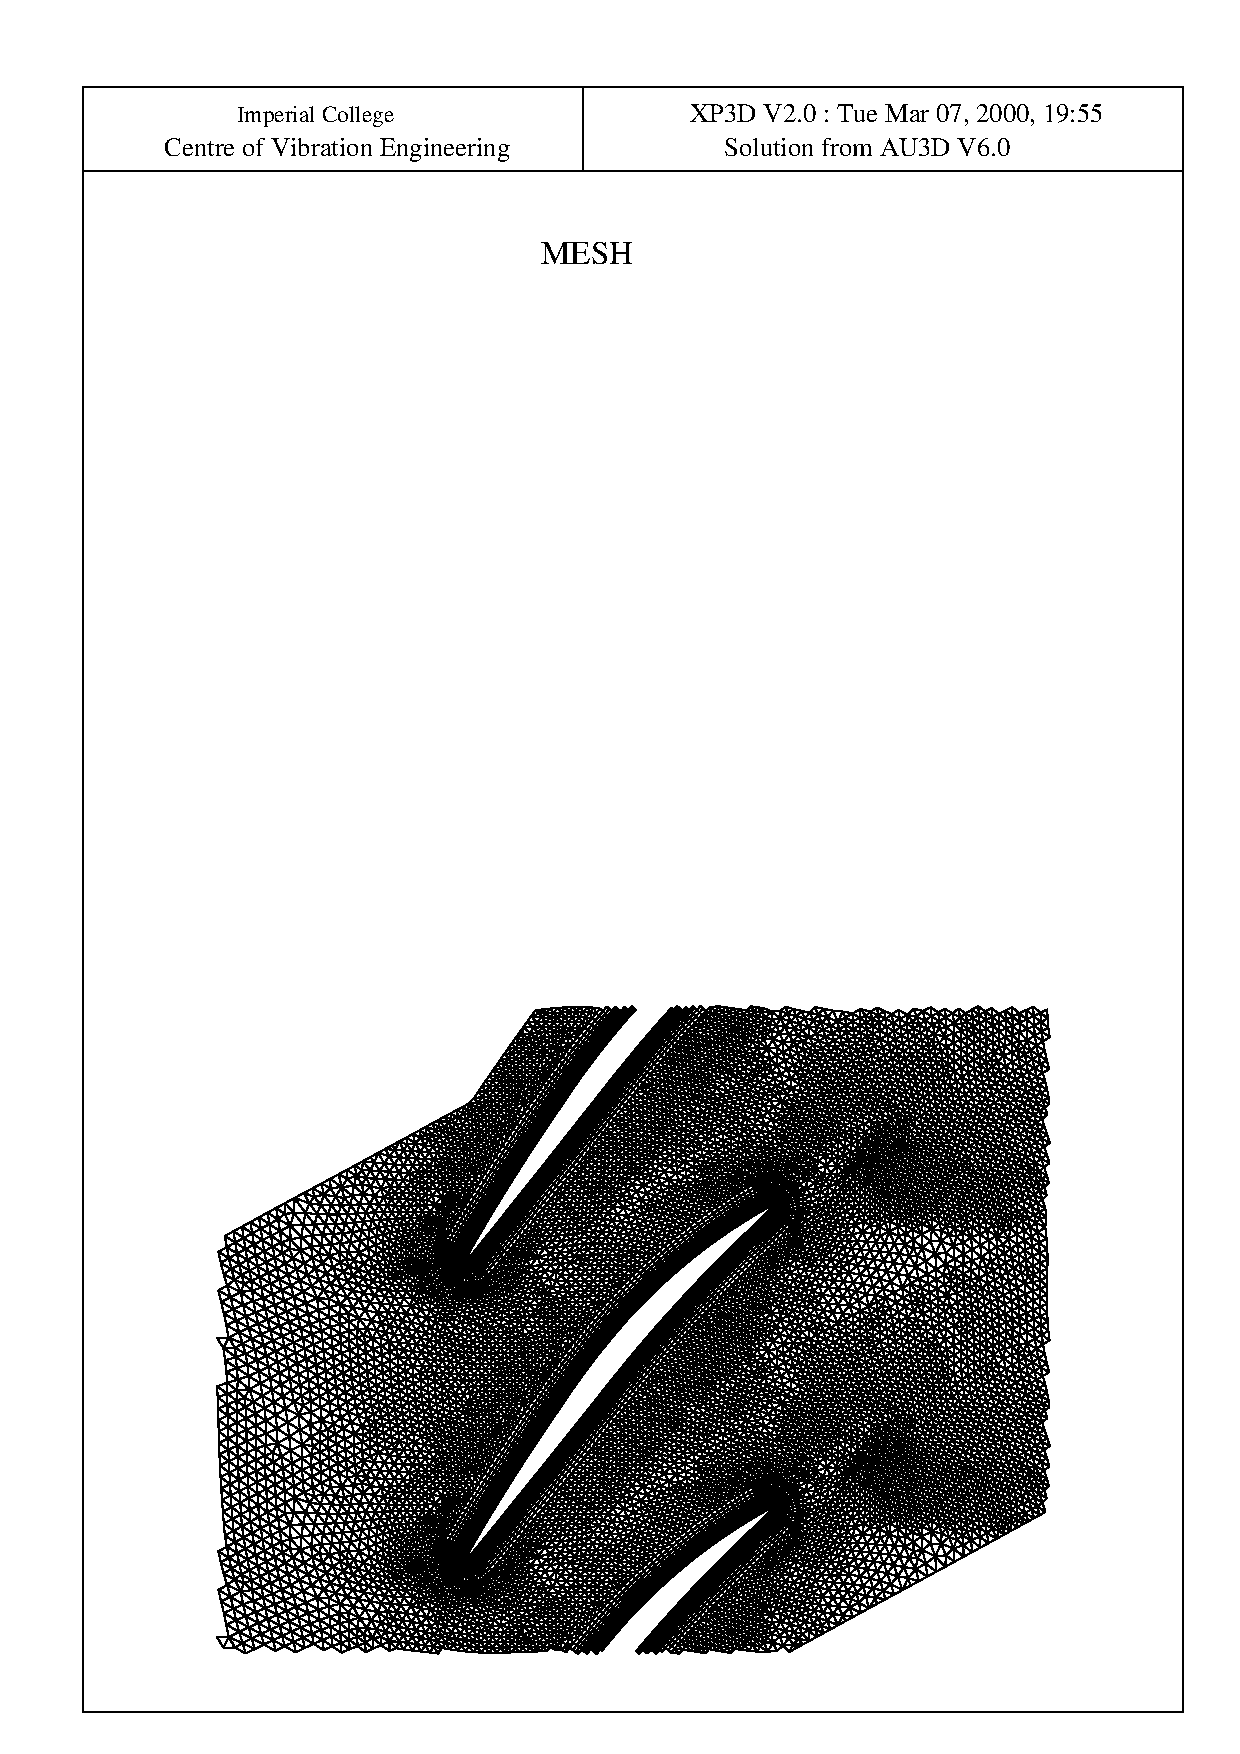
\includegraphics[width=85mm,clip=t]{CHAP_NONLIN/FIGURE/rot37_mesh4.pdf}}
      \vspace{-4mm}\\
    \subfigure[Tip gap view]
       {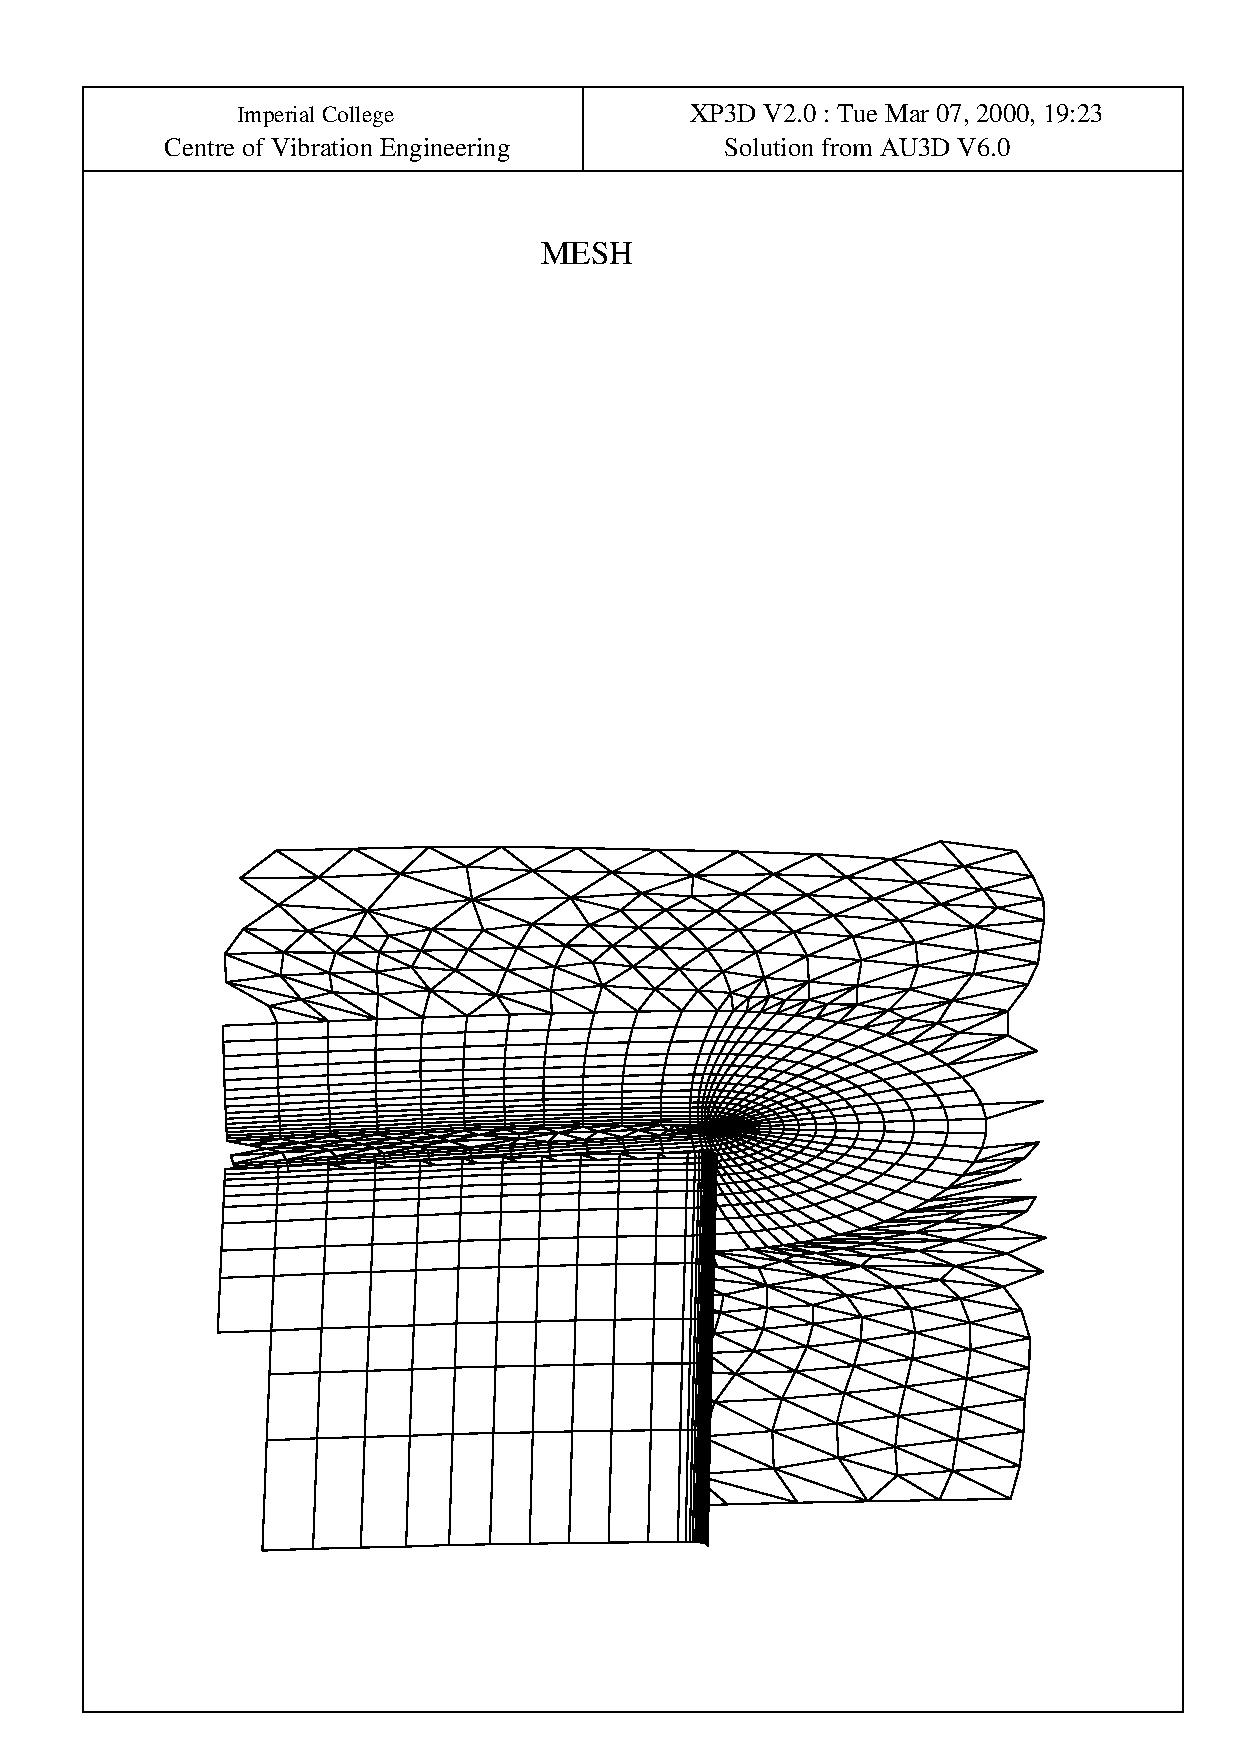
\includegraphics[width=55mm,clip=t]{CHAP_NONLIN/FIGURE/rot37_mesh3.pdf}}
        &
    \subfigure[$x-r$ view]
       {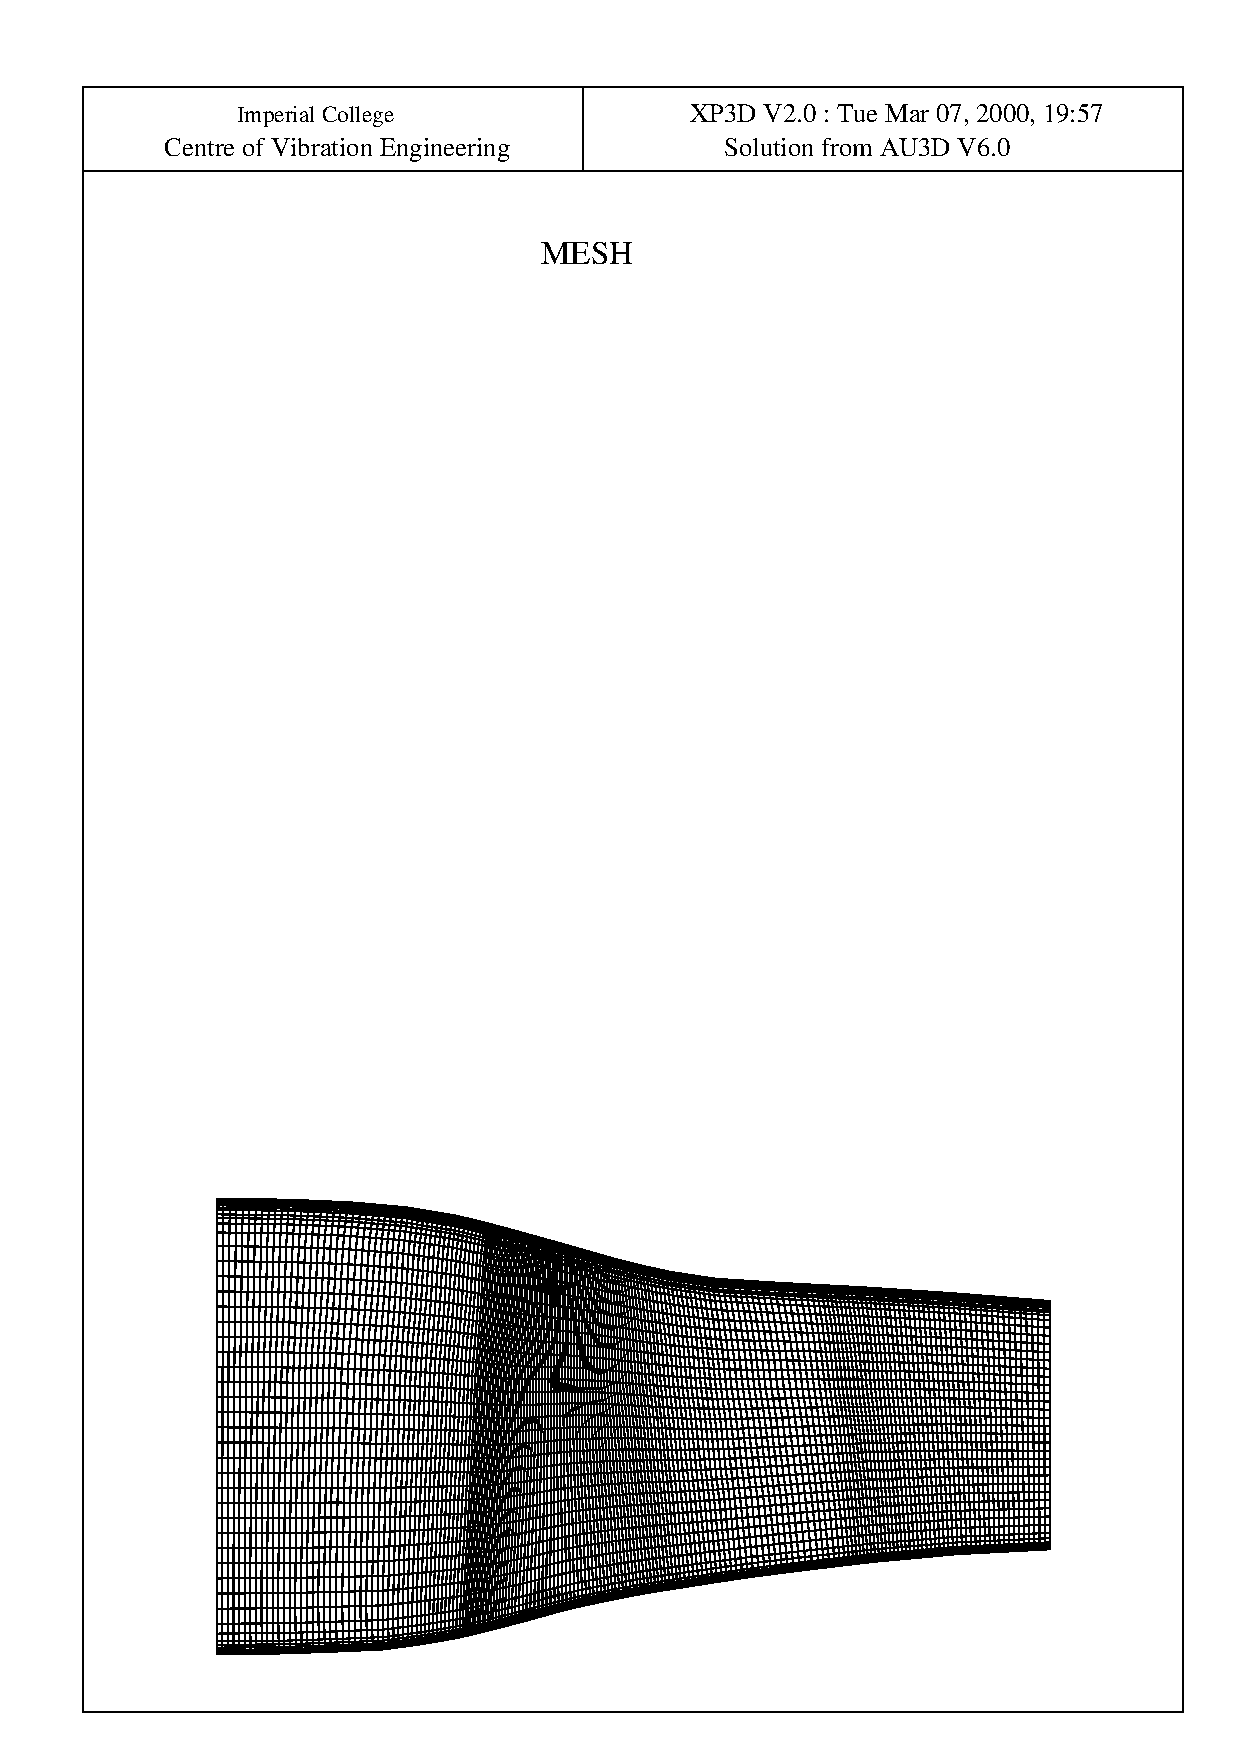
\includegraphics[width=85mm,clip=t]{CHAP_NONLIN/FIGURE/rot37_mesh2.pdf}}
  \end{tabular}
 \end{center}
 \vspace{-8mm}
 \caption{NASA Rotor 37: computational mesh}
 \label{rot37_mesh.fig}
\end{figure}
%
 Views of the computational mesh,
 generated with the semi-structured mesh generator
 LEVMAP described in chapter \ref{mesh.chap}
 (Sbardella et al. \citeyearNP{Luca:9}),
 are shown in Fig. \ref{rot37_mesh.fig}.
 The computational domain extends axially from station 1 in Fig.
 \ref{rot37_geo.fig} up to $x=10.67\ cm$ which corresponds to
 station 4 (not shown in Fig. \ref{rot37_geo.fig}). It contains 174,900 hexahedra
 in the boundary layer reagion and 607,067 wedges in the rest of the domain for
 a total number of point of 504,946. The boundary layer mesh does not resolve
 the viscous sublayer thus calculations with wall-slip condition
 (\ref{flow_tangency1.eq}) and wall-shear
 stresses evaluated using the low of the wall are considered here.
 As shown in Fig. \ref{rot37_geo.fig}c, the tip clearance flows will be modelled
 in a straightforward way by simply meshing the gap and setting the rotation
 speed at the casing to zero.
 At the hub section the reagion $x < -0.264\ cm$, $x > 4.521\ cm$,
 is not rotating so the rotational speed is also set to zero.
%
\begin{figure}
 \begin{center}
  \begin{tabular}{cc}
    \subfigure[$95\%$ span]
       {\includegraphics[width=60mm,clip=t]{FIGURE/CHAP2/rot37_cont_95.pdf}}
        &
    \subfigure[$97\%$ span]
       {\includegraphics[width=60mm,clip=t]{FIGURE/CHAP2/rot37_cont_97.pdf}}
       \vspace{-4mm} \\
    \subfigure[$99\%$ span]
       {\includegraphics[width=60mm,clip=t]{FIGURE/CHAP2/rot37_cont_99.pdf}}
        &
    \subfigure[Tip gap]
       {\includegraphics[width=60mm,clip=t]{FIGURE/CHAP2/rot37_cont_gap.pdf}}
  \end{tabular}
 \end{center}
 \vspace{-8mm}
 \caption{Rotor 37: Mach number contours}
 \label{rot37_mach.fig}
\end{figure}
%

%
%
%
%
\subsection{Impulsively accelerated flat plate}
\label{accelerated_flat_plate.subsec}
%
 To demonstrate the capability of the present method for unsteady flow,
 the solution of an impulsively accelerated flat plate in the laminar regime
 is presented. This example is also known as Stokes first problem
 and an analytical solution for incompressible flow is available
 (Schlichting \citeyearNP{Schlichting}, Mattioli \citeyearNP{Mattioli:1}).
 This analytical solution shows that the time dependent
 solution collapses to a single solution of nondimensional velocity versus
 the similarity parameter $\eta$ defined as

%
\beq
  \eta = \frac{y}{2\sqrt{\nu t}}
  \label{stokes_first1.eq}
\eeq
%
 where $y$ is the normal distance from the flat plate, $\nu$ is the kinematic
 viscosity and $t$ is the physical time. The analytical solution take the
 simple form

%
\beq
  \frac{u}{u_\infty} = {\tt erf}\left(\eta\right)
  \label{stokes_first2.eq}
\eeq
%
 where $\tt erf$ represents the error function (Schlichting \citeyearNP{Schlichting}).
%
\begin{figure}
 \begin{center}
  \begin{tabular}{c}
    \subfigure[Velocity profiles]
       {\includegraphics[width=110mm,clip=t]{CHAP_NONLIN/FIGURE/flat_sol.pdf}}
        \\
    \subfigure[Convergence history]
       {\includegraphics[width=110mm,clip=t]{CHAP_NONLIN/FIGURE/flat_res.pdf}}
  \end{tabular}
 \end{center}
 \vspace{-8mm}
 \caption{Impulsively started flat plate. $M_\infty = 0.2$, $Re_\infty = 40,000$.
          Velocity profiles and residual history}
 \label{flat_impul.fig}
\end{figure}

 Three calculations were performed with the present method with 1, 5 and 10
 physical time steps to reach the same physical time $t = 0.001\ sec$.
 The maximum ratio between the physical and pseudo time step, $\Delta t/\Delta\tau$,
 was of around 17,000 for the case where a single time step was used to reached
 $t = 0.001\ sec$. Fig. \ref{flat_impul.fig}a shows the comparison between
 the numerical and analytical solutions. As expected, the smaller the physical time
 step, the better the agreement.
 If one used an explicit method to calculate the unsteady flow at the same physical
 time level, than it should have performed around 15,000 time steps using
 a CFL number of 1.5. For the case of 5 time step the convergence of
 (\ref{Dual_time_stepping_3.eq}) for a given time level was obtained with $\approx 15$
 W multigrid cycles using four grids. In terms of CPU time this means
 that with 5 time steps the present method was $\approx 120$ times faster than
 an explicit Runge-Kutta integration method.

 Fig. \ref{flat_impul.fig}b shows the comparison of the
 residual within a given physical time step, using a single grid and a four grids
 W-type cycle. As one would expected, the convergece to a new physical time level
 improves if more the one grid are used. However such improvement does not
 compare with the one obtained for steady-state computations.
 Convergence histories similar to the one
 shown in Fig. \ref{flat_impul.fig}b represents the best result
 obtained for unsteady flows.

%
%
%
%
\subsection{Vortex shedding past a cylinder}
\label{vortex_shedding_cylinder.subsec}
%
\begin{figure}
 \begin{center}
  \begin{tabular}{cc}
    \subfigure[Computational grid: 17391 points]
        {\includegraphics[height=60mm,clip=t]{CHAP_NONLIN/FIGURE/cil_me1.pdf}}
        &
    \subfigure[Zoom view at leading edge]
        {\includegraphics[height=60mm,clip=t]{CHAP_NONLIN/FIGURE/cil_me0.pdf}}
  \end{tabular}
 \end{center}
 \vspace{-5mm}
 \caption{Circular cylinder. Computational mesh}
 \label{cil_mesh1.fig}
\end{figure}
%
 This test case is intended to predict the natural vortex shedding
 past a cylinder in a laminar incompressible flow regime.
 Vortex shedding is one of many viscous flows which, though posed
 with fixed and steady boundary conditions, evolve into unsteady
 motions because of flow instability.
 If one consider a circular cylinder with diameter $d$, then
 the incompressible flow field generated by a uniform
 velocity at infinity $u_\infty$
 is dependent solely upon the Reynolds number $Re_d$

%
\beq
  Re_d = \frac{\rho_\infty u_\infty d}{\mu_\infty}
\eeq
%
 If $Re_d < 40$ the flow is steady. If $Re_d > 40$
 the flow becomes unstable and consequently unsteady when
 $Re_d > 50$. The flow field is caracterised by a unsteady wake
 which consists of pairs of vortices shed alternately from the
 upper and lower part of the cylinder surface.
 If $50 < Re_d < 150$ such a wake structure is well organised and is
 called Karman vortex sheet after a paper by Karman (1911) explaining
 this alternation to be a stable configuration for vortex pairs
 (Schlichting \citeyearNP{Schlichting}).
 An important feature of this flow is that the dimensionless
 cylinder frequency or Stroudal number

%
\beq
  St = \frac{f d}{u_\infty}
\eeq
%
 remains constant $\approx 0.21$ for $100 < Re_d < 10,000$. Thus, in this
 Reynolds number range, the shedding cycle takes place during the time
 that the free-stream moves approximately five cylinder diameters.
%
\begin{figure}[ht]
 \begin{center}
  \begin{tabular}{ccc}
    \subfigure[Grid 2: 4308 cells]
       {\includegraphics[width=45mm,clip=t]{CHAP_NONLIN/FIGURE/cil_me2.pdf}}
        &
    \subfigure[Grid 3: 1095 cells]
       {\includegraphics[width=45mm,clip=t]{CHAP_NONLIN/FIGURE/cil_me3.pdf}}
        &
    \subfigure[Grid 4: 283 cells]
       {\includegraphics[width=45mm,clip=t]{CHAP_NONLIN/FIGURE/cil_me4.pdf}}
  \end{tabular}
 \end{center}
 \vspace{-5mm}
 \caption{Circular cylinder. Agglomerated grids}
 \label{cil_mesh2.fig}
\end{figure}

 Fig. \ref{cil_mesh1.fig} shows the computational mesh used for this test case,
 it contains 2280 quadrilaterals in the boundary layer and 29863
 triangles in the rest of the domain for a total number of point of 17391.
 Fig. \ref{cil_mesh2.fig} shows the three agglomerated grids used in the time
 accurate multigrid algorithm.
 Four different calculations were performed for various Reynolds numbers
 with an inlet Mach number of 0.2
 and the computed Stroudal number is reported in Fig. \ref{stroudal.fig}a together
 with the experimental value of 0.21. The comparison is satisfactory for
 all four test cases.
 Fig. \ref{stroudal.fig}b reports the evolution in time of the pressure coefficient
 at a point in the wake close to the cylinder. The time history refers to three cycles of
 oscillations after a periodic flow conditions is reached. The very periodic behaviour
 of the flow is evident and proves the robustness and accuracy of the scheme.
%
\begin{figure}
 \begin{center}
  \begin{tabular}{c}
    \subfigure[Computed Stroudal number]
       {\includegraphics[width=110mm,clip=t]{CHAP_NONLIN/FIGURE/stroud.pdf}}
        \\
    \subfigure[$c_p$ evolution]
       {\includegraphics[width=110mm,clip=t]{CHAP_NONLIN/FIGURE/prehis.pdf}}
  \end{tabular}
 \end{center}
 \vspace{-5mm}
 \caption{Circular cylinder. Computed Stroudal number and $c_p$ evolution}
 \label{stroudal.fig}
\end{figure}
%

 The time step for those calculations was set to have 50 divisions over a cycle.
 This correspond to a local CFL number between two in the far field and three
 thousand in the boundary layer region.
%
\begin{figure}[ht]
 \begin{center}
  \begin{tabular}{c}
    \subfigure[$Re_d = 400$]
       {\begin{tabular}{ccc}
         \includegraphics[width=45mm,clip=t]{CHAP_NONLIN/FIGURE/cil2.pdf}
         &
         \includegraphics[width=45mm,clip=t]{CHAP_NONLIN/FIGURE/cil3.pdf}
         &
         \includegraphics[width=45mm,clip=t]{CHAP_NONLIN/FIGURE/cil4.pdf}
        \\
         Time 1 & Time 2 & Time 3
        \\
         \includegraphics[width=45mm,clip=t]{CHAP_NONLIN/FIGURE/cil5.pdf}
         &
         \includegraphics[width=45mm,clip=t]{CHAP_NONLIN/FIGURE/cil6.pdf}
         &
         \includegraphics[width=45mm,clip=t]{CHAP_NONLIN/FIGURE/cil1.pdf}
        \\
         Time 4 & Time 5 & Time 6
       \end{tabular}}
     \\
    \subfigure[$Re_d = 4000$]
       {\begin{tabular}{ccc}
         \includegraphics[width=45mm,clip=t]{CHAP_NONLIN/FIGURE/cim2.pdf}
         &
         \includegraphics[width=45mm,clip=t]{CHAP_NONLIN/FIGURE/cim3.pdf}
         &
         \includegraphics[width=45mm,clip=t]{CHAP_NONLIN/FIGURE/cim4.pdf}
        \\
         Time 1 & Time 2 & Time 3
        \\
         \includegraphics[width=45mm,clip=t]{CHAP_NONLIN/FIGURE/cim5.pdf}
         &
         \includegraphics[width=45mm,clip=t]{CHAP_NONLIN/FIGURE/cim6.pdf}
         &
         \includegraphics[width=45mm,clip=t]{CHAP_NONLIN/FIGURE/cim1.pdf}
        \\
         Time 4 & Time 5 & Time 6
       \end{tabular}}
  \end{tabular}
 \end{center}
 \vspace{-5mm}
 \caption{Circular cylinder. Instantaneous particle traces}
 \label{cil_sol1.fig}
\end{figure}
%

 Figs. \ref{cil_sol1.fig} reports the instantaneous
 particle traces in six instants over a cycle (the seventh position would be
 equivalent to the first) for two different $Re_d$.
 The shedding of the vortex is evident as well as the mechanism of their formation
 with a vortex merging. This is evident in Fig. \ref{cil_sol1.fig}a between instants
 3 and 4, and 6 and 1.
 It is worth to note the different pattern followed by the vortices for the two
 Reynolds number under consideration. For $Re_d= 400$ the
 shedding structure is well organised while for $Re_d= 4,000$
 the inertial forces play a more important role in the wake flow with formations
 of large recirculation bubbles which are propagated with small dissipation.
%

%
%
%
%
\subsection{Transonic buffeting over a bicircular airfoil}
\label{transonic_buffeting.subsec}
%
 Starting for about 1976, several experiments were
 carried out on transonic buffeting over bicircular-arc airfoils
 at NASA Ames research center with the intent to provide
 basic data to guide further development of computer codes
 (McDevitt et al. \citeyearNP{McDevitt:1}).
 The wind tunnel used for those experiments was designed for
 this purpose in order to minimize upper and lower wall
 interference effects. The tests were conducted at free-stream
 Reynolds numbers, based on airfoil chord length, ranging from 1
 to 17 million. The test Mach number was varied from near the critical
 value of 0.71 to the highest possible without the airfoil chocking
 the channel.
 McDevitt et al. \citeyear{McDevitt:1} presented unsteady results for
 a biconvex circular-arc airfoil with thickness-chord ratio of 0.18.
 The nominal test Mach for this airfoil is 0.775 and the wind
 tunnel end walls were designed to minimize wall effects for this flow
 condition.
%
%
\begin{figure}[ht]
 \begin{center}
  \begin{tabular}{ccc}
    \subfigure[Time 1]
       {\includegraphics[width=45mm,clip=t]{CHAP_NONLIN/FIGURE/arc1.pdf}}
        &
    \subfigure[Time 2]
       {\includegraphics[width=45mm,clip=t]{CHAP_NONLIN/FIGURE/arc2.pdf}}
        &
    \subfigure[Time 3]
       {\includegraphics[width=45mm,clip=t]{CHAP_NONLIN/FIGURE/arc3.pdf}}
        \vspace{-4mm}\\
    \subfigure[Time 4]
       {\includegraphics[width=45mm,clip=t]{CHAP_NONLIN/FIGURE/arc4.pdf}}
        &
    \subfigure[Time 5]
       {\includegraphics[width=45mm,clip=t]{CHAP_NONLIN/FIGURE/arc5.pdf}}
        &
    \subfigure[Time 6]
       {\includegraphics[width=45mm,clip=t]{CHAP_NONLIN/FIGURE/arc6.pdf}}
        \vspace{-4mm}\\
    \subfigure[Time 7]
       {\includegraphics[width=45mm,clip=t]{CHAP_NONLIN/FIGURE/arc7.pdf}}
        &
    \subfigure[Time 8]
       {\includegraphics[width=45mm,clip=t]{CHAP_NONLIN/FIGURE/arc8.pdf}}
        &
    \subfigure[Time 9]
       {\includegraphics[width=45mm,clip=t]{CHAP_NONLIN/FIGURE/arc9.pdf}}
        \vspace{-4mm}\\
    \subfigure[Time 10]
       {\includegraphics[width=45mm,clip=t]{CHAP_NONLIN/FIGURE/arc10.pdf}}
        &
    \subfigure[Time 11]
       {\includegraphics[width=45mm,clip=t]{CHAP_NONLIN/FIGURE/arc11.pdf}}
        &
    \subfigure
       {\includegraphics[width=45mm,clip=t]{CHAP_NONLIN/FIGURE/arc12.pdf}}
  \end{tabular}
 \end{center}
 \vspace{-5mm}
 \caption{Bicircular airfoil. $M_\infty = 0.775$,
          $Re_\infty = 7\cdot10\se{6}$. Instantaneous Mach number contours}
 \label{arc_sol1.fig}
\end{figure}
%
 At a free-stream Reynolds number of 7 million, experiments suggest
 transonic buffeting at a free stream Mach number in the range
 from 0.76 to 0.78. On the contrary, the calculations show
 unsteadiness in the Mach number range from 0.765 up to 0.83.
 The computed buffeting reduced frequency $\pi f c/u\sm{\infty}$
 matches the experimental one of $\approx 0.5$.

 Fig. \ref{arc_sol1.fig} reports instantaneous Mach number contours
 in eleven instants over a cycle while Fig. \ref{arc_sol2.fig}a
 shows the average and range of pressure coefficient distribution
 in the airfoil surface.
%
\begin{figure}
 \begin{center}
  \begin{tabular}{c}
    \subfigure[pressure coefficient distribution]
     {\includegraphics[height=90mm,clip=t]{CHAP_NONLIN/FIGURE/arc_uns.pdf}}
        \\
    \subfigure[pressure coefficient evolution]
     {\includegraphics[height=90mm,clip=t]{CHAP_NONLIN/FIGURE/arc_per.pdf}}
  \end{tabular}
 \end{center}
 \vspace{-5mm}
 \caption{Bicircular airfoil. Computed pressure coefficient}
 \label{arc_sol2.fig}
\end{figure}
%
 Fig. \ref{arc_sol2.fig}b reports the evolution in time of the pressure
 coefficient at a point in the airfoil corresponding to $x/c = 0.7$.
 The time history refers to three cycles of oscillation after a periodic
 flow  condition is reached. The calculations were performed
 using roughly 45 divisions over a cycle
 (as indicated in Fig. \ref{arc_sol2.fig}b). This correspond to a local CFL
 number between 0.1 in the far-field and 10,000 in the boundary layer.
%
%

%
%
\section{Concluding Remarks}
\headb{Nonlinear Navier-Stokes solver}{Concluding remarks}
%
\begin{itemize}
%
 \item
 A FV scheme for the solution of the Favre averaged
 Navier-Stokes equations has been presented. The method employs an edge-based
 data structure as well as  a nearest-neighbour stencil for the discretisation of
 the Laplacian operator. The method enables the use of 2D and 3D
 unstructured, structured or block structured mixed-element grids without any modifications
 to the numerical scheme.
% 
\item
 A drawback of this approach is the need to evaluate the mixed
 derivative terms of the viscous fluxes by using a standard FV method which does not yield
 a nearest neighbour stencil.
 However, in cases where the viscous effects are in the boundary layer
 only, such terms are
 very small and hence the method is expected to be well suited to
 engineering applications.
%
\item
 The same time relaxation multigrid algorithm has been applied to both
 steady and unsteady time-marching aerodynamics. The benefit of unconditional
 stability has been demonstrated by computing unsteady
 viscous flow with time-steps corresponding to CFL numbers on the
 range 1000 - 10,000.
%
\item
 The multigrid technique efficiently performs for steady-state flow
 computations even though its robustness needs to be improved for 3D
 turbulent flow simulations.
 For time-marching unsteady flows, the multigrid technique does not
 perform as well. Convergence histories similar to the one
 shown in Fig. \ref{flat_impul.fig}b represents the best result
 obtained. The reason for such a break down is not clear. However
 the stability restriction in (\ref{local_time_step_2.eq}) could
 play and important part near the far-field boundaries.
%
\item
 For unsteady computations, an attractive way forward could be the
 implementation of an adaptive scheme which select different
 time-marching techniques in different zones depending on the
 local situation.
%
\item
 The scheme produces good and stable results for highly distorted
 meshes as demonstrated by Sbardella \& Imregun \citeyear{Luca:11}. 
%
\end{itemize}
%

%
%
%
%%%%%%%%%%%%%%%%%%%%%%%%%%%%%%%%%%%%%%%%%%%%%%%%%%%%%%%%%%%%%%%%%%%%%%%%
\chapter{Linearised Unsteady Navier-Stokes Solver}
\label{linear.chap}
\heada{Linearsed Navier-Stokes solver}
\setcounter{footnote}{0}
%%%%%%%%%%%%%%%%%%%%%%%%%%%%%%%%%%%%%%%%%%%%%%%%%%%%%%%%%%%%%%%%%%%%%%%%
%
%
%
 This Chapter extends the hybrid grid flow solver of in the previous
 Chapter, to a time-linearised version of the unsteady Favre-averaged Navier-Stokes
 equations.
 The linearised unsteady viscous flow equations are derived by assuming small
 harmonic perturbations from a steady-state flow and
 the resulting equations are solved using a pseudo-time marching technique.
 Such an approach enables the same numerical algorithm to be used for both
 the non-linear steady and the linearised unsteady flow computations.
 An important feature of the work is the full linearisation of
 the Spalart-Allmaras turbulence model. 
 The methodology was validated for a number of 2D test cases such as linear
 flat-plate cascades and flat plates with laminar boundary layers.
 A more advanced study is given for two different flow regimes past a
 turbine cascade, the so-called 11th International Standard Configuration,
 for which there are both steady and unsteady flow measurements.
 Linearised unsteady flow predictions were discussed for several modelling
 levels: inviscid, viscous with frozen turbulence and fully turbulent viscous.
 The findings highlighted the need for a full linearisation in cases where
 the steady-state flow exhibits significant viscous effects such as
 separation and recirculation.
%
\section{Towards Viscous linearised representations}
\headb{Linearsed Navier-Stokes solver}{Towards Viscous linearised representations}
%
 In Section \ref{linear_methods.subsec} a literary survey on linearised
 method is given. The methods presented were based on an inviscid
 flow representation and thus they cannot deal with cases where viscous
 effects are important:
 shock-boundary layer interaction, flow separation and recirculation.
 It should be noted that such features are particularly important for turbomachinery
 unsteady flows because most investigations are conducted at off-design conditions. 
 For instance, generally speaking, fan blades do not encounter flutter problems at
 the design speed but part-speeds may cause some concern.
 The flow behaviour at these lower speeds is dominated by viscous effects
 and hence the linearised analysis tools must somewhat include the necessary features.
 
 One of the first time-linearised Navier-Stokes analyses of a cascade unsteady flow was
 reported by Cizmas \& Hall \citeyear{Hall:7}. The computational domain was
 divided into two parts: a viscous flow near the airfoil and in the wake region,
 and an inviscid flow in the rest of the domain.
 The viscous flow was modelled using a finite difference discretisation of the
 boundary layer equations while the inviscid flow was modelled
 using a finite element discretisation of the full potential equation.
 However the analysis was limited to incompressible flows and to prescribed
 boundary layer assumption. Ning \& He \citeyear{He:3} presented a novel quasi 3D non-linear
 harmonic Euler/Navier-Stokes method which combines the computational efficiency
 of linearised techniques and some of the accuracy of non-linear formulations.  
 Holmes et al. \citeyear{Holmes:1} are amongst the first researchers to present a 3D
 time-linearised Navier-Stokes analysis with a $k-\omega$ turbulence model.
 Their results were limited to flows with a thin attached boundary layer and
 whether or not the turbulence model itself needed to be linearised was discussed
 in detail. Although this issue will be dealt with later in this Chapter,
 an overview will be given here. 
 Avoiding the linearisation of the turbulence model and using the mean-flow
 values for the eddy viscosity, the so-called frozen turbulence model,
 is relatively straightforward.
 On the other hand, the linearisation of the turbulence model may require
 significant algebra and coding effort. The mathematical formulation of a specific turbulence
 model and its mesh density requirement near the blade surface are further
 important considerations. For instance, a very fine mesh requirement may well
 negate some of the computational advantages. 
 In any case, an important contribution is made by Clark \& Hall \citeyear{Hall:8}
 who reported a 2D linearised Navier-Stokes analysis using the one-equation
 Spalart-Allmaras \citeyear{Spalart:1} turbulence model.
 They predicted the aeroelasticity behaviour of a fan blade
 at some off-design condition which involved high incidence and 
 flow separation over much of the suction surface.
 Their results showed good overall agreement with the available experimental data.

 The present Chapter describes a 2D/3D finite-volume (FV) scheme for a full discretisation of
 the time-linearised Navier-Stokes equations. The important features of the present work
 are the discretisation of the domain via a single, unified edge-data structure
 for mixed-element meshes and the use of a Laplacian weight which
 results in nearest neighbour stencils. Furthermore,  the one-equation turbulence model of
 Spalart-Allmaras \citeyear{Spalart:1}, which has the form of a sixth conservation equation,
 was linearised for a consistent formulation. Such a unified approach
 allows the use of 2D and 3D structured, unstructured or block-structured
 grids with mixed elements under the same numerical scheme.
 The results were validated against available analytical and experimental data.
 The differences between linearising inviscid, frozen turbulence and fully-turbulence
 models are discussed in some detail for the case of the
 $11\se{th}$ International Standard Configuration. 
%
%
%
%
%
\section{Time-linearised Navier-Stokes Equations}
\headb{Linearsed Navier-Stokes solver}{Linearisation}
%
 This Section deals with the linearisation of the 3D
 unsteady, compressible, Favre-averaged Navier-Stokes
 equations (\ref{conservative_formulation_nl.eq}) and
 the correspondent boundary conditions. Since (\ref{conservative_formulation_nl.eq})
 as been written in a ALE formulation, the inclusion of linearised
 blade oscillation becomes straightforward by simply linearising the
 mesh motion as well as the flow equations.
%
%
\subsection{Linearisation}
\label{linearisation.subsec}
%
 The linearisation of the governing equations around a steady-state
 solution starts by expressing the conservation variables and
 the coordinates as a sum of a mean steady-state value and a
 small perturbation:

%
\beq
 \vec{x}\left(\overline{\vec{x}}, t\right) &=&
  \overline{\vec{x}} + \widetilde{\vec{x}}\left(\overline{\vec{x}},t\right) \\
 {\bf U}\left(\overline{\vec{x}}, t\right) &=&
  \overline{\bf U}\left(\overline{\vec{x}}\right) +
  \widetilde{\bf U}\left(\overline{\vec{x}}, t\right)
\eeq
%
 It is then possible to express the unsteady flux vector $\vec{\bf F}$ in
 (\ref{nonlinear_inviscid_flux.eq}) as a summation of three different terms:

%
\beq
  \vec{\bf F} = \overline{\vec{\bf F}} + \widetilde{\vec{\bf F}} 
              - \widetilde{\vec{\bf F}}{\scriptstyle g}
  \label{flux_decomposition.eq}
\eeq
%
 where  $\overline{\vec{\bf F}}$ represents the mean steady value of the
 inviscid fluxes, $\widetilde{\vec{\bf F}}$ is the unsteady part
 of the inviscid fluxes which does not include the grid motion while
 $\widetilde{\vec{\bf F}}{\scriptstyle g}$ includes the unsteady terms
 due to the grid motion only.
 To first order, using (\ref{relative_velocity.eq}) and
 (\ref{nonlinear_inviscid_flux.eq}) the terms above can be expressed as:

%
\beq
  \overline{\vec{\bf F}} &=& \overline{\bf U}
                  \left(\overline{\vec{v}} - \vec{\Omega}\times\overline{\vec{x}}\right)
                          + \overline{\vec{\bf F}}{\scriptstyle p}
  \label{steady_flux_1.eq}\\
  \widetilde{\vec{\bf F}} &=&
                         \widetilde{\bf U}\left(\overline{\vec{v}} -
                              \vec{\Omega}\times\overline{\vec{x}}\right)
                       + \overline{\bf U}\ \widetilde{\vec{v}}
                       + \widetilde{\vec{\bf F}}{\scriptstyle p}
  \label{unsteady_flux_1.eq}\\
  \widetilde{\vec{\bf F}}{\scriptstyle g} &=& \overline{\bf U}\left(
                              \vec{\Omega}\times\widetilde{\vec{x}} +
                                      \frac{d\widetilde{\vec{x}}}{d t}\right)
\eeq
%
 Substituting in (\ref{conservative_formulation_nl.eq}), one obtains:

%
\beq
  \fpdt{} \int_{{\cal V}} \left(\overline{\bf U} + \widetilde{\bf U}\right)
  \left(d\overline{\cal V} + d\widetilde{\cal V}\right) + 
  \oint_{\cal S} \left(\overline{\vec{\bf F}} + \widetilde{\vec{\bf F}}
  -  \widetilde{\vec{\bf F}}{\scriptstyle g}\right)
  \cdot \left(\overline{\vec{n} d{\cal S}} +
  \widetilde{\vec{n} d{\cal S}}\right)&-&
  \nonumber \\
  \frac{1}{Re}\oint_{\cal S} \left(\overline{\vec{\bf G}} + \widetilde{\vec{\bf G}}\right)
  \cdot \left(\overline{\vec{n} d{\cal S}} +
  \widetilde{\vec{n} d{\cal S}}\right) - 
  \int_{{\cal V}} \left(\overline{\bf S} + \widetilde{\bf S}\right)
  \left(d\overline{\cal V} + d\widetilde{\cal V}\right) &=& 0
  \label{linear_equation_1.eq}
\eeq
%
 By dropping the steady-state terms which must always satisfy
 (\ref{conservative_formulation_nl.eq})
 and by neglecting second-order terms like $\widetilde{\bf U}d\widetilde{\cal V}$,
 (\ref{linear_equation_1.eq}) becomes:

%
\beq
  \fpdt{} \int_{{\cal\overline{V}}} \widetilde{\bf U} d\overline{\cal V} &+&
  \oint_{\cal\overline{S}} \left(\widetilde{\vec{\bf F}} -
                                    \frac{1}{Re}\widetilde{\vec{\bf G}}\right)
  \cdot\overline{\vec{n} d{\cal S}} -
  \int_{{\cal\overline{V}}} \widetilde{\bf S}d\overline{\cal V} =
  \int_{\overline{\cal V}} \overline{\bf S} d\widetilde{\cal V}
 - \fpdt{} \int_{\overline{\cal V}} \overline{\bf U} d\widetilde{\cal V}
   \nonumber \\
 &-&  \oint_{\overline{\cal S}}\left(\overline{\vec{\bf F}} -
                                \frac{1}{Re}\overline{\vec{\bf G}}\right)
      \cdot\widetilde{\vec{n} d{\cal S}}
  + \oint_{\overline{\cal S}}\widetilde{\vec{\bf F}}{\scriptstyle g}
                          \cdot\overline{{\vec{n}} d{\cal S}}
 \label{linear_equation_2.eq}
\eeq
%
 The system of equations in  (\ref{linear_equation_2.eq}) is linear in the sense
 that all the coefficients multiplying the unsteady flow term $\widetilde{\bf U}$
 depend upon the steady-state flow  term 
 $\overline{\bf U}$ and geometric properties but not on time.
 In other words, a general solution of (\ref{linear_equation_2.eq})
 can be represented via the following summations:

%
 \beq
   \widetilde{\vec{x}}\left(\overline{\vec{x}},t\right) &=&
   {\tt Re} \sum\sm{\omega}
   \widehat{\vec{x}}\left(\overline{\vec{x}},\omega\right) e\se{-i\omega t}
   \label{x_amplitude.eq} \\
   \widetilde{\bf U}\left(\overline{\vec{x}},t\right) &=&
   {\tt Re} \sum\sm{\omega}
   \widehat{\bf U}\left(\overline{\vec{x}},\omega\right) e\se{-i\omega t}
   \label{u_amplitude.eq}
\eeq
%
 where $\widehat{\vec{x}}$ represents the first-order complex amplitude
 of grid motion about the mean position $\overline{\vec{x}}$, and 
 $\widehat{\bf U}$ represent the complex amplitude of the small
 unsteady perturbation of the conservation variables.
 By substituting the assumed solutions (\ref{x_amplitude.eq}) and 
 (\ref{u_amplitude.eq}) for a single reduced frequency $\omega$ into
 the linearised system of equations (\ref{linear_equation_2.eq}), 
 one obtains:

%
\beq
 &&\oint_{\overline{\cal S}}\left(\widehat{\vec{\bf F}}-\frac{1}{Re}\widehat{\vec{\bf G}}\right)
 \cdot \overline{\vec{n} d{\cal S}}  -
 \int_{\overline{\cal V}} \left(i\omega \widehat{\bf U} + \widehat{\bf S}\right)
 d\overline{\cal V} =
 \int_{\overline{\cal V}} \left(i\omega \overline{\bf U} + \overline{\bf S}\right)
 d\widehat{\cal V} - \nonumber \\
 &&\oint_{\overline{\cal S}}\left(\overline{\vec{\bf F}}-\frac{1}{Re}\overline{\vec{\bf G}}\right) \cdot
      \widehat{{\vec{n}} d{\cal S}}
 + \oint_{\overline{\cal S}}
  \overline{\bf U}\left(\vec{\Omega}\times\widehat{\vec{x}}
                    -i\omega\widehat{\vec{x}}\right)
  \cdot \overline{{\vec{n}} d{\cal S}}
 \label{linear_equation_3.eq}
\eeq
%
 In equation (\ref{linear_equation_3.eq}) the left-hand side contains
 homogeneous terms only, while the right-hand side contains non-homogeneous
 terms which depend on the (known) steady-state flow and the prescribed grid
 motion. The non-homogeneous terms are identically zero if there is no grid
 motion ($\widehat{\vec{x}}={0}$), as is the case for  forced response problems.
 
 Since the Jacobian with respect to the steady-state flow variables are real
 quantities, the homogeneous terms of the form $i\omega\int\sm{\overline{\cal V}} \widehat{\bf U}
 d\overline{\cal V}$, which represent the time rate of change of the perturbed
 conservation variables, couple the real and imaginary parts of the
 perturbed flow equations.

 Indicating with $\widehat{\bf H}\left(\overline{U},\widehat{\bf x}\right)$ the
 summation of the non-homogeneous terms on the right-hand side of (\ref{linear_equation_3.eq})
 and introducing a pseudo-time derivative so that standard time-marching algorithms can be used,
 (\ref{linear_equation_3.eq}) becomes:

%
\beq
 \fpd{}{\tau}\int\sm{\overline{\cal V}} \widehat{\bf U} d\overline{\cal V} +
 \oint_{\overline{\cal S}}\left(\widehat{\vec{\bf F}}-\frac{1}{Re}\widehat{\vec{\bf G}}\right)
 \cdot \overline{\vec{n} d{\cal S}}  -
 \int_{\overline{\cal V}} \left(i\omega \widehat{\bf U} + \widehat{\bf S}\right)
 d\overline{\cal V} =
 \widehat{\bf H}\left(\overline{\bf U}, \widehat{\vec{x}}\right)
 \label{linear_equation_4.eq}
\eeq
%
%
%
\subsection{Boundary conditions}
%
 There are five different sets of boundary conditions: flow tangency for inviscid flow
 calculations, no-slip condition for viscous flow calculations,
 periodic boundaries, inflow and outflow.
%
\subsubsection{Flow tangency}
%
 The flow tangency condition at the solid walls is expressed by the requirement
 that there is no flow through the surface of the moving wall.
 Therefore, the local fluid velocity relative to the moving wall has no
 component normal to the wall. Mathematically this can be expressed as:

%
\beq
  \vec{u}\cdot\vec{n} =
 \left(\vec{v} - \vec{\Omega}\times\vec{x} - \frac{d \vec{x}}{d t}\right)\cdot\vec{n}
 = 0
\eeq
%
 Linearising and keeping zeroth- and first-order terms gives
 the mean flow and the linearised tangency conditions respectively:

%
\beq
  \left(\overline{\vec{v}} - \vec{\Omega}\times\overline{\vec{x}}\right)
  \cdot\overline{\vec{n}} &=& 0
  \label{flow_tangency_1.eq} \\
  \left(\widehat{\vec{v}} - \vec{\Omega}\times\widehat{\vec{x}}
        + i \omega \widehat{\vec{x}}\right)\cdot\overline{\vec{n}} +
  \left(\overline{\vec{v}} - \vec{\Omega}\times\overline{\vec{x}}\right)
  \cdot\widehat{\vec{n}} &=& 0
  \label{flow_tangency_2.eq}
\eeq
%
 Applying condition (\ref{flow_tangency_2.eq}) to the evaluation
 of the flux term for a solid wall surface yields:

%
\beq
 \oint\sm{wall}\left[\widehat{\vec{\bf F}} -
 \overline{\bf U}\left(\vec{\Omega}\times\widehat{\vec{x}}
                     - i\omega\widehat{\vec{x}}\right)\right]
          \cdot\overline{\vec{n}d{\cal S}} +
 \oint\sm{wall} \overline{\vec{\bf F}} \cdot\widehat{\vec{n}d{\cal S}}
 \nonumber\\
 =
 \left[
 \begin{array}{c}
 0 \\ \widehat{p}\ \overline{n\sm{x} d{\cal S}}+\overline{p}\ \widehat{n\sm{x} d{\cal S}}
   \\ \widehat{p}\ \overline{n\sm{y} d{\cal S}}+\overline{p}\ \widehat{n\sm{y} d{\cal S}}
   \\ \widehat{p}\ \overline{n\sm{z} d{\cal S}}+\overline{p}\ \widehat{n\sm{z} d{\cal S}}
   \\ \widehat{p}\ \left(\vec{\Omega}\times\overline{\vec{x}}\right)
      \cdot\overline{\vec{n}d{\cal S}} + 
      \overline{p} \left[\left(\vec{\Omega}\times\overline{\vec{x}}\right)
                          \cdot\widehat{\vec{n}d{\cal S}} +
                          \left(\vec{\Omega}\times\widehat{\vec{x}}
                                -i\omega\widehat{\vec{x}}\right)
                          \cdot\overline{\vec{n}d{\cal S}}\right]
 \end{array}
 \right]
\eeq
%
%
\subsubsection{No-slip condition}
%
 The no-slip condition at the solid walls is expressed by the requirement that the local
 fluid velocity relative to the moving wall must be zero.
 Mathematically this can be expressed as:

%
\beq
  \vec{u} = \vec{v} - \vec{\Omega}\times\vec{x} - \frac{d \vec{x}}{d t} = 0
\eeq
%
 As before, linearising and keeping zeroth- and first-order terms gives
 the mean flow and the linearised no-slip conditions respectively:

%
\beq
  \overline{\vec{v}} - \vec{\Omega}\times\overline{\vec{x}} &=& 0
  \label{no_slip_1.eq} \\
  \widehat{\vec{v}} - \vec{\Omega}\times\widehat{\vec{x}}
        + i \omega \widehat{\vec{x}} &=& 0
  \label{no_slip_2.eq}
\eeq
%
%
\subsubsection{Periodic boundaries}
%
 The periodic boundary conditions are somewhat more complicated than those for
 the steady-state flow equations. 
 In a flutter application, the blade may
 oscillate with a non-zero phase shift with respect to its neighbours.
 Similarly, in a wake/rotor interaction,  there will be a phase difference 
 in the unsteady pressure distributions experienced by neighbouring rotor blades
 if there is no one-to-one correspondence between the wakes and the rotor blades.
 Such phase differences are represented by the interblade phase angle $\phi$.
 Using an axisymmetric coordinate system, the periodic boundary condition can be
 written as: 

%
\beq
  \widehat{\bf U}_{\theta_0 + \Delta \theta} = 
  \exp{\left(-i\phi\right)}\widehat{\bf U}_{\theta_0}
\eeq
%
 where $\widehat{\bf U}$ is the state variable at position $\theta_0$,
 $\Delta \theta$ representing the angular pitch of the blade-to-blade passage.
 The same equation can be used for a 2D cascade, by replacing
 $\theta_0$ and $\Delta \theta$ by $y_0$ and $P$ in a Cartesian coordinate system.
 
%
\subsubsection{Inflow and outflow boundaries}
%
 Unsteady flow computations require non-reflecting boundary conditions
 at the far-field boundaries to prevent spurious inwards reflections of outgoing waves.
 The single-frequency non-reflecting boundary conditions of
 Giles \citeyear{Giles:6} will be used here.
 These boundary conditions are constructed with the aid of 
 the 1D characteristic variables. The equations relating the harmonic primitive
 variables and the harmonic characteristic variables can be written as:

%
\beq
  \left[
    \begin{array}{c}
    \widehat{w}\sm{1} \\
    \widehat{w}\sm{2} \\
    \widehat{w}\sm{3} \\
    \widehat{w}\sm{4} \\
    \widehat{w}\sm{5}
    \end{array}
  \right] &=&
  \left[
    \begin{array}{ccccc}
     -\overline{c}\se{2} & 0 & 0 & 0 & 1\\
      0 & 0 & \overline{\rho c} & 0 & 0\\
      0 & 0 & 0 & \overline{\rho c} & 0\\
      0 & \overline{\rho c} & 0 & 0 & 1\\
      0 &-\overline{\rho c} & 0 & 0 & 1
    \end{array}
  \right]
  \left[
    \begin{array}{c}
     \widehat{\rho} \\
     \widehat{v\sm{x}} \\
     \widehat{v\sm{\theta}} \\
     \widehat{v\sm{r}} \\
     \widehat{p}
    \end{array}
  \right] 
\eeq
%
 The first characteristic variable represents the 1D entropy wave, the second and third
 represent the two 1D vorticity waves while the fourth and the fifth characteristic
 variables represent the forward and backward 1D pressure waves.
 These 1D characteristic variables can be expressed as a
 sum of spatial harmonics satisfying the periodicity condition with the correct
 interblade phase angle.

%
\beq
  \widehat{w}\sm{n} = \sum\sm{m} \widehat{w}\sm{n}\se{m}
  \exp\left[i\theta\frac{2\pi m - \phi}{\Delta \theta}\right]
\eeq
%
 Following the work of Giles \citeyear{Giles:6},
 it is possible to express the $m$-th harmonic of the
 incoming 1D characteristic variables as a function of the
 $m$-th harmonic of the outgoing ones.
 At the inflow, the boundary condition is:

%
\beq
  \left[
   \begin{array}{c}
    \widehat{w}\sm{1}\se{m} \\
    \widehat{w}\sm{2}\se{m} \\
    \widehat{w}\sm{3}\se{m} \\
    \widehat{w}\sm{4}\se{m}
   \end{array}
  \right] =
  \left[
   \begin{array}{c}
    0 \\
    \frac{\left(1-M\sm{x}\right)\beta\sm{m}}
         {1-M\sm{\theta}\beta\sm{m}+T\sm{m}}\\
    0 \\
    \frac{\left(1-M\sm{x}\right)\se{2}\beta\sm{m}\se{2}}
         {\left(1-M\sm{\theta}\beta\sm{m}+T\sm{m}\right)\se{2}}
   \end{array}
  \right]
   \widehat{w}\sm{5}\se{m}
  \label{inflow_bc}
\eeq
%
 while at the outflow it becomes:

%
\beq
  \widehat{w}\sm{5}\se{m} = \frac{2-M\sm{x}\beta\sm{m}}
                            {1-M\sm{\theta}\beta\sm{m}+T\sm{m}}
                            \widehat{w}\sm{2}\se{m} +
                            \frac{1-M\sm{\theta}\beta\sm{m}-T\sm{m}}
                            {1-M\sm{\theta}\beta\sm{m}+T\sm{m}}
                            \widehat{w}\sm{4}\se{m}
  \label{outflow_bc}
\eeq
%
 In both cases $\beta\sm{m}$ is an inverse reduced frequency defined by:

%
\beq
  \beta\sm{m} = \frac{2\pi m - \phi}{r\Delta\theta\omega}\overline{c}
\eeq
%
 where $\overline{c}$ is the average speed of sound and $r\Delta\theta$
 is the product of radius and angular pitch. $T\sm{m}$ in (\ref{outflow_bc})
 is defined by:

%
\beq
  T\sm{m}\se{2} &=& \left(1-M\sm{\theta}\beta\sm{m}\right)\se{2} - 
                    \left(1-M\sm{x}\se{2}\right)\beta\sm{m}\se{2}\\
  T\sm{m} &=& \left\{
  \begin{array}{ll}
  {\rm sign}\left(1-M\sm{\theta}\beta\sm{m}\right)\sqrt{T\sm{m}\se{2}}
  &\ \ \ T\sm{m}\se{2}>0\\
  {\rm sign}\left(\omega\right)i\sqrt{-T\sm{m}\se{2}}
  &\ \ \ T\sm{m}\se{2}<0
  \end{array}
  \right.
\eeq
%
 Giles \citeyear{Giles:6} suggested that the periodic boundary conditions should be
 lagged when using pseudo-time marching, though this was not found necessary with
 the particular solver used here.
 Equations (\ref{inflow_bc}) \& (\ref{outflow_bc}) are the exact 2D analytical
 boundary conditions. These can be extended to 3D
 problems by imposing them in a strip-theory fashion at each spanwise radial station
 at the domain boundary,
 the so-called quasi-3D non-reflecting boundary conditions (Saxer \& Giles 
 \citeyearNP{Giles:7}).
 One limitation of such an approach is the inherent assumption 
 that the radial variation in the mean and unsteady
 flow fields is considerably smaller than that in the tangential direction. 
 This is not necessarily the case in aeroacoustic applications.
 A more general 3D approach, developed by
 Hall et al. \citeyear{Hall:5}, is a mixed analytical/numerical
 boundary condition treatment.
 The assumption is that the mean flow field is axisymmetric and 
 uniform in the axial direction, but may have significant radial variation.
 The unsteady flow-field is decomposed into Fourier modes in the circumferential
 direction, and a radial eigenvalue problem is solved to determine the wave numbers
 and the radial mode shapes of the unsteady flow modes. The modal information is
 then used to construct highly non-reflective boundary conditions. However, in some
 special cases, the identification of the incoming and outgoing modes may be difficult
 and truncation errors may affect the scheme adversely. Nevertheless, the approach is
 probably the most general boundary condition treatment that is currently available.
%
%
%
\section{Numerical Implementation}
\headb{Linearsed Navier-Stokes solver}{Numerical Implementation}
%
 The extension of the finite volume FV edge-based scheme, described
 in Chapter \ref{flow_model.chap}, to the linearised equations
 will be described in this Section.
 Similar to (\ref{semi_discrete_nl.eq}), the semi-discrete form
 of (\ref{linear_equation_4.eq}) takes the form:

%
\beq
  \frac{\partial \left({\cal V}\sm{I}\widehat{\bf U}\sm{I}\right)}{\partial \tau}
 +\sum\sm{s=1}\se{m\sm{I}} \left[\left|\vec{\eta}\sm{IJs}\right|
  \left(\widehat{\cal F}\sm{IJs}-\widehat{\cal G}{\scriptstyle m}\sm{IJs}\right) -
  \tau\sm{IJs} \widehat{\cal G}{\scriptstyle l}\sm{IJs}\right]
  = {\cal V}\sm{I}
 \left(i\omega\widehat{\bf U}\sm{I}+\widehat{\bf S}\sm{I}+\widehat{\bf H}\sm{I}\right)
  \label{semi_discrete_linear.eq}
\eeq
%
%
%
\subsection{Inviscid fluxes}
%
 The discretisation of the inviscid flow terms in (\ref{semi_discrete_linear.eq})
 is given by:

%
\beq
  \sum\sm{s=1}\se{m\sm{I}} \left|\vec{\eta}\sm{IJs}\right|
  \widehat{\cal F}\sm{IJs}
 \label{inviscid_contribution}
\eeq
%
 where $\widehat{\cal F}\sm{IJs}$ represents the inviscid flux function along edge
 $IJ\sm{s}$
 which is obtained using a central difference scheme with added
 matrix artificial dissipation. This artificial dissipation
 is a blend of second and fourth order differences. The fourth order
 terms ensure the stability of the scheme in smooth regions of the flow,
 while the second order terms are required to damp numerical oscillations
 in the vicinity of discontinuities.
 The inviscid flux function is expressed as:

%
\beq
  \widehat{\cal F}\sm{IJs} = \frac{\widehat{\vec{\bf F}}\sm{I}
  + \widehat{\vec{\bf F}}\sm{Js}}{2}
  \cdot\frac{\vec{\eta}\sm{IJs}}{\left|\vec{\eta}\sm{IJs}\right|}
  - \widehat{\cal D}\sm{IJs}
\eeq
%
 where the linearised artificial dissipation
 $\widehat{\cal D}\sm{IJs}$ along the edge $IJ\sm{s}$ is
 given by:

%
\beq
  \widehat{\cal D}\sm{IJs} = \frac{1}{2}
  \left|\overline{\bf A}\sm{IJs}\right|
  \left[\overline{\psi}\ \Delta \widehat{\bf U}
 -\epsilon\sm{4}\left(1-\overline{\psi}\right) \Delta {\cal L}\left(\widehat{\bf U}\right)\right]
  \label{artifical_diffusion}
\eeq
%
 The difference operator $\Delta$ is given in (\ref{difference_operator.eq}).
 $\left|\overline{\bf A}\sm{IJs}\right|$ is the standard Roe matrix
 (Roe \citeyearNP{Roe:1}) between the two steady-state stages
 $\overline{\bf U}\sm{I}$ and $\overline{\bf U}\sm{Js}$;
 $\epsilon\sm{4}\approx 1/16$ is the fourth order artificial dissipation
 coefficient. ${\cal L}$ is the pseudo-Laplacian operator
 reported in (\ref{pseudo_lapl_nl.eq}) while
 $\overline{\psi}$ represents the limiting function which varies between
 0 and 1 and it is required in order to switch the scheme to first order
 ($\overline{\psi} = 1$) in the vicinity of discontinuities. This limiter is
 computed for the steady-state flow only and its expression is given by
 (\ref{limiter_mult_1.eq}) and (\ref{limiter_mult_2.eq}).
%
%
\subsection{Viscous terms}
%
 The viscous fluxes associated with the mixed derivatives
 ${\cal G}{\scriptstyle m}$ in (\ref{semi_discrete_linear.eq})
 are treated in the same way as their inviscid
 counterparts and their contribution to (\ref{semi_discrete_linear.eq})
 is given by:

%
\beq
  \widehat{\cal G}{\scriptstyle m}\sm{IJs} = \frac{1}{Re}
  \left(\widehat{\vec{\bf G}}{\scriptstyle m}\sm{I} +
        \widehat{\vec{\bf G}}{\scriptstyle m}\sm{Js}\right)\cdot
  \frac{\vec{\eta}\sm{IJs}}{\left|\vec{\eta}\sm{IJs}\right|}
  \label{viscous_mix}
\eeq
%
 where

%
\beq
  \widehat{\vec{\bf G}}{\scriptstyle m} = 
  \left.\widehat{\vec{\bf G}}{\scriptstyle m}\right|\sm{\overline{\mu}} +
  \left.\widehat{\vec{\bf G}}{\scriptstyle m}\right|\sm{\Delta\overline{\bf U}}
  \label{gm_def}
\eeq
%
 The first term on the left-hand side of (\ref{gm_def}) contains the contribution 
 due to the  gradients of the unsteady flow velocity and temperature at constant viscosity $\mu$.
 The second term takes into account the variation of the unsteady viscosity only.
 The Laplacian terms are treated in a different way in order to
 improve both the accuracy and the robustness of the numerical scheme.
 In (\ref{semi_discrete_linear.eq}), these terms take the form:

%
\beq
  \widehat{\cal G}{\scriptstyle l}\sm{IJs} =
      \left.\widehat{\cal G}{\scriptstyle l}\sm{IJs}\right|\sm{\overline{\mu}} +
      \left.\widehat{\cal G}{\scriptstyle l}\sm{IJs}\right|\sm{\Delta\overline{\bf U}}
  \label{linear_viscous_split.eq}
\eeq
%
 where

%
\beq
 \left.\widehat{\cal G}{\scriptstyle l}\sm{IJs}\right|\sm{\overline{\mu}}
 &=& \frac{1}{Re} \left[
 \begin{array}{c}
  0 \\ \overline{\mu}\sm{IJs}\ \Delta \widehat{v}\sm{1}
    \\ \overline{\mu}\sm{IJs}\ \Delta \widehat{v}\sm{2}
    \\ \overline{\mu}\sm{IJs}\ \Delta \widehat{v}\sm{3}
    \\ \left(\overline{\mu\vec{v}}\right)\sm{IJs}\cdot \Delta \widehat{\vec{v}}
       + \frac{\gamma}{\gamma\!-\!1}\left(\frac{\overline{\mu}\sm{l}}{Pr\sm{l}}\!+\
         \frac{\overline{\mu}\sm{t}}{Pr\sm{t}}\right)\sm{IJs}\Delta \widehat{T}
 \end{array}
 \right]
 \label{linear_laplacian_1.eq}\\
 \left.\widehat{\cal G}{\scriptstyle l}\sm{IJs}\right|\sm{\Delta\overline{\bf U}}
 &=& \frac{1}{Re} \left[
 \begin{array}{c}
  0 \\ \widehat{\mu}\sm{IJs}\ \Delta \overline{v}\sm{1}
    \\ \widehat{\mu}\sm{IJs}\ \Delta \overline{v}\sm{2}
    \\ \widehat{\mu}\sm{IJs}\ \Delta \overline{v}\sm{3}
    \\ \left(\overline{\mu}\widehat{\vec{v}}+\widehat{\mu}\overline{\vec{v}}\right)\sm{IJs}
       \cdot \Delta \overline{\vec{v}}
       + \frac{\gamma}{\gamma\!-\!1}\left(\frac{\widehat{\mu}\sm{l}}{Pr\sm{l}}\!+\
         \frac{\widehat{\mu}\sm{t}}{Pr\sm{t}}\right)\sm{IJs}\Delta \overline{T}
 \end{array}
 \right]
 \label{linear_laplacian_2.eq}
\eeq
%
 The subscript $IJs$ indicates an arithmetic mean over nodes $I$ and $Js$
 as indicated in (\ref{side_average.eq}) and $\Delta$ is given in 
 (\ref{difference_operator.eq}).

 The evaluation of terms $\left.\widehat{\vec{\bf G}}{\scriptstyle m}\right|\sm{\Delta\overline{\bf U}}$
 and $ \left.\widehat{\cal G}{\scriptstyle l}\sm{IJs}\right|\sm{\Delta\overline{\bf U}}$ requires
 the linearisation of the turbulence model used
 in the steady flow solver.
 If these terms are neglected, the linearised viscous terms can still be represented by
 simply using the mean-flow values for the eddy viscosity,
 the so-called frozen turbulence approach.
 Such a scheme is relatively simple to implement for any turbulence model,
 while a full linearisation will depend on the particular type of
 the turbulence model used.
 A linearised version of the Spalart-Allmaras \citeyear{Spalart:1} turbulence
 model is given in the Appendix \ref{turbulence.chap}.
%
%
\subsection{Time integration}
%
 The pseudo-time derivative introduced in (\ref{linear_equation_4.eq})
 allows the use of standard time-marching algorithms when solving
 the linearised equations. A compact form of (\ref{semi_discrete_linear.eq})
 can be written as

%
\beq
 \frac{\partial \left({\cal V}\sm{I}\widehat{\bf U}\sm{I}\right)}{\partial \tau} = 
 {\bf R}\sm{I}\left(\widehat{\bf U}\right)
\eeq
%
 Many different approaches are possible.
 For instance,  Hall \& Clark \citeyear{Hall:4} use an explicit Lax-Wendroff technique
 together with local time-stepping and multigrid in order to accelerate convergence to
 a steady-state. Marshall \& Giles \citeyear{Giles:8} use an explicit multistage Runge-Kutta
 technique with local-time stepping.
 Montgomery \& Verdon \citeyear{Verdon:3} proposed a two-point
 backward implicit difference and the expansion
 of the residual about the {\em n}th time level.

 Here, the same preconditioned multigrid algorithm developed for steady-state
 and non-linear unsteady time-marching aerodynamics is used.
 In a compact form the algorithm is written as

%
\beq
  \left[\overline{\bf P}\right]\se{-1}L\sm{\tau} \delta \widehat{\bf U}\sm{I} =
  {\bf R}\sm{I}\left(\widehat{\bf U}\right)
  \label{time_linear.eq}
\eeq
%
 $L\sm{\tau}$ represents a multistage Runge-Kutta operator while
 $\left[\overline{\bf P}\right]\se{-1}$
 represents a preconditioner developed for accelerating steady-state
 calculations, evaluated using the steady-state unknowns.

 Such a preconditioned Runge-Kutta relaxation algorithm is used as
 a smoother in an agglomeration multigrid algorithm described in Appendix
 \ref{multigrid.chap}.
%
%
%
%
%
\section{Test Cases}
\headb{Linearsed Navier-Stokes solver}{Test Cases}
%
 This Section presents three different test cases for the validation of the
 present method. The first test case is a comparison against the classical subsonic
 flat plate cascade theory of Smith \citeyear{Smith:1},
 the so-called LINSUB benchmark code (Whitehead \citeyearNP{Whitehead:1}).
 The second test case checks the computational results against the
 asymptotic analytical solution derived by Lighthill \citeyear{Lighthill:1}
 for an unsteady laminar flow. The third test case examines the implications
 of using inviscid, frozen-turbulence and fully-turbulent models when linearising
 the unsteady flow over a transonic  turbine blade, the so-called 11th International
 Standard Configuration  (Fransson et al. \citeyearNP{Bolcs:2}).
%
%
%
\subsection{Linear flat-plate cascade}
\label{LINSUB.subsec}
%
\begin{figure}
  \begin{center}
  \begin{tabular}{cc}
    \subfigure[Geometry]
      {\includegraphics[width=70mm,clip=t]{CHAP_LINEAR/FIGURE/lins_geom.pdf}
       \hspace{0mm}} &
    \subfigure[Computational domain (2,232 points)]
      {\hspace{0mm}
        \includegraphics[width=70mm,clip=t]{CHAP_LINEAR/FIGURE/lins_mesh.pdf}}
   \end{tabular}
 \end{center}
 \vspace{-8mm}
 \caption{Flat plate cascade. Geometry and computational domain}
 \label{linsub_geom_mesh.fig}
\end{figure}
%
%
\begin{figure}
  \begin{center}
  \begin{tabular}{c}
    \subfigure[Real part]
       {\includegraphics[width=110mm,clip=t]{CHAP_LINEAR/FIGURE/lins_wake1.pdf}
       \hspace{0mm}} \\
    \subfigure[Imaginary part]
      {\hspace{0mm}
        \includegraphics[width=110mm,clip=t]{CHAP_LINEAR/FIGURE/lins_wake2.pdf}}
   \end{tabular}
 \end{center}
 \vspace{-8mm}
 \caption{LINSUB test case. Pressure jump on flat plate due to wake/rotor interaction
          ($\omega = \pi$, $\phi = -90\se{o}$)}
 \label{linsub_wake.fig}
\end{figure}
%
\begin{figure}
  \begin{center}
  \begin{tabular}{c}
    \subfigure[Real part]
       {\includegraphics[width=110mm,clip=t]{CHAP_LINEAR/FIGURE/lins_pres1.pdf}
       \hspace{0mm}} \\
    \subfigure[Imaginary part]
      {\hspace{0mm}
        \includegraphics[width=110mm,clip=t]{CHAP_LINEAR/FIGURE/lins_pres2.pdf}}
   \end{tabular}
 \end{center}
 \vspace{-8mm}
 \caption{LINSUB test case. Pressure jump on flat plate due to upstream acoustic wave
          ($\omega = 2$, $\phi = 0\se{o}$)}
 \label{linsub_pres.fig}
\end{figure}
%
\begin{figure}
  \begin{center}
  \begin{tabular}{c}
    \subfigure[Real part]
       {\includegraphics[width=110mm,clip=t]{CHAP_LINEAR/FIGURE/lins_bend1.pdf}
       \hspace{0mm}} \\
    \subfigure[Imaginary part]
      {\hspace{0mm}
        \includegraphics[width=110mm,clip=t]{CHAP_LINEAR/FIGURE/lins_bend2.pdf}}
   \end{tabular}
 \end{center}
 \vspace{-8mm}
 \caption{LINSUB test case. Pressure jump on flat plate due to bending oscillation
          ($\omega = 2$, $\phi = 90\se{o}$)}
 \label{linsub_bend.fig}
\end{figure}
%
%
 Small-amplitude perturbations of a uniform, inviscid steady-state flow past an
 unloaded flat-plate cascade are studied first.  Such cascades can  be used for a
 variety of applications: wake/blade interaction, potential/blade interaction, aeroelasticity
 studies by including the blade's bending and torsional motion. The main aerodynamic
 parameters are the Mach number, reduced frequency, pitch-to-chord ratio, stagger
 angle and the interblade phase angle.

 Three different disturbances were studied for  a pitch-to-chord ratio of 0.5,
 a stagger angle of $30\se{o}$ and a mean-flow Mach number of 0.7.
 For all three cases, the results were checked against the benchmark LINSUB code
 by plotting the real and imaginary parts of the (complex) unsteady pressure difference across
 the plate.  The geometry and the computational domain  are
 shown in Fig. \ref{linsub_geom_mesh.fig}. The mesh has high resolution around the
 trailing and leading edges in order to handle the singularities which occur
 in these regions.

 The first disturbance simulates a wake/blade interaction, an incoming
 sinusoidal wake with a reduced frequency of $\pi$ being specified at the inflow boundary.
 The  interblade phase angle is $-90\se{o}$. Fig. \ref{linsub_wake.fig}
 shows  excellent agreement between the present method and the benchmark program LINSUB.
 The second disturbance simulates potential/blade interaction,  an
 incoming pressure wave with a reduced frequency of $2.0$ being specified
 at the outflow boundary. The interblade phase angle is $0\se{o}$.
 Fig. \ref{linsub_pres.fig} shows excellent agreement between the present method and the
 benchmark program LINSUB.
 The last disturbance  studied is for a bending motion with a reduced frequency of
 $2.0$ and an interblade phase angle of $90\se{o}$. Once again, excellent agreement
 is observed from Fig. \ref{linsub_bend.fig}.
%

%
%
%
\subsection{Unsteady laminar boundary layer on a flat plate}
\label{unsteady_flat_linear.subsec}
%
\begin{figure}
  \begin{center}
  \begin{tabular}{cc}
    \subfigure[Computational mesh (5954 points)]
       {\includegraphics[width=80mm,clip=t]{CHAP_LINEAR/FIGURE/flat_laminar_mesh1.pdf}
       \hspace{0mm}} &
    \subfigure[trailing edge]
      {\hspace{0mm}
        \includegraphics[width=40mm,clip=t]{CHAP_LINEAR/FIGURE/flat_laminar_mesh2.pdf}}
   \end{tabular}
 \end{center}
 \vspace{-7mm}
 \caption{Computational domain for laminar flow over a flat plate cascade}
 \label{flat_laminar_linear_mesh.fig}
\end{figure}
%
 This test case studies an unsteady laminar
 boundary layer with fluctuations in external velocity.
 The computational mesh is shown in Fig. \ref{flat_laminar_linear_mesh.fig}.
 The boundary layer region is discretised using 15 layers of quadrilateral elements,
 while the rest of the domain consists of triangles.
 The pitch to chord ratio of this cascade is unity so that the flow is
 as close as possible to that over an isolated flat plate.
 The steady-state flow  over an unstaggered flat plate cascade was obtained for
 a Mach number of 0.2.  The freestream Reynolds number is 60,000. Such a case is
 well within the incompressible flow regime, thus enabling  a meaningful comparison
 with the Blasius solution.  Indeed, the computed steady-state  velocity profile and
 the skin friction coefficient are found to be in very good agreement with the
 incompressible laminar boundary layer theory of  Blasius (Fig. \ref{flat_laminar_steady.fig}).
 Once the steady-state flow has been validated, the next stage is to study a
 velocity perturbation of the form:

%
\beq
  u = \varepsilon u\sm{\infty} e\se{-i\omega t}
\eeq
%
 where $u\sm{\infty}$ is the freestream velocity and $\varepsilon$ a small value ($\ll 1$).
 The disturbance is along the plate, in the freestream direction, denoted by co-ordinate $x$.
 Lighthill's \citeyear{Lighthill:1} theory provides two asymptotic values for
 the unsteady skin friction coefficient, one for very small and the other for very
 large reduced frequency values. Fig. \ref{flat_laminar_linear_sol.fig}a
 shows the wall shear stress amplitude variation with reduced frequency $\omega x/u\sm{\infty}$
 while Fig. \ref{flat_laminar_linear_sol.fig}b shows the computed phase angle
 between shear stress and external velocity. As expected, the computed results
 become asymptotic for the limiting cases of very small and very large reduced
 frequency. Similar comparisons between numerical results and Lighthill's theory
 are also reported by Cebeci \citeyear{Cebeci:1}.
%
%
%
\begin{figure}
  \begin{center}
  \begin{tabular}{c}
    \subfigure[Velocity profile]
       {\includegraphics[width=110mm,clip=t]{CHAP_LINEAR/FIGURE/flat_laminar_vel.pdf}
       \hspace{0mm}} \\
    \subfigure[Skin friction coefficient]
      {\hspace{0mm}
        \includegraphics[width=110mm,clip=t]{CHAP_LINEAR/FIGURE/flat_laminar_cff.pdf}}
   \end{tabular}
 \end{center}
 \vspace{-7mm}
 \caption{Steady laminar flow over a cascade of flat plates}
 \label{flat_laminar_steady.fig}
\end{figure}
%
\begin{figure}
  \begin{center}
   \begin{tabular}{c}
    \subfigure[Amplitude]
       {\includegraphics[width=110mm,clip=t]{CHAP_LINEAR/FIGURE/flat_laminar_ampli.pdf}
       \hspace{0mm}} \\
    \subfigure[Phase angle with respect to external velocity fluctuation]
      {\hspace{0mm}
        \includegraphics[width=110mm,clip=t]{CHAP_LINEAR/FIGURE/flat_laminar_phase.pdf}}
   \end{tabular}
 \end{center}
 \vspace{-7mm}
 \caption{Unsteady wall shear stresses for an oscillating laminar boundary layer}
 \label{flat_laminar_linear_sol.fig}
\end{figure}
%

%
%
%
%
\subsection{Turbine cascade}
\label{stand11.subsec}
%
%
\begin{figure}
 \centerline{\includegraphics[width=120mm,clip=t]{CHAP_LINEAR/FIGURE/mesh_11th.pdf}}
 \caption{$11^{th}$ Standard configuration. Viscous mesh}
 \label{mesh_11th.fig}
\end{figure}
%
 In this Section the steady and unsteady flow due to bending motion
 of a turbine blade in the direction normal to its chord is analysed.
 The turbine blade geometry under consideration represents the
 $11\se{th}$ International Standard Configuration which have been
 studied for several flow regimes by Fransson et al.
 \citeyear{Bolcs:2}\footnote{The data for the International Standard Configurations
 can be found at {\bf http://www.egi.kth.se/ekv/stcf/} }.
 Two particular flows  will be considered here:
 a subsonic attached flow  and a transonic flow showing a separation
 bubble on the suction surface.
 Fig. \ref{mesh_11th.fig} shows the computational mesh used for all viscous
 calculations. There are 9,312 quadrilaterals in the
 boundary layer region and 7,751 triangles in the rest of the domain, the total  number
 of points being 13,481. A second mesh, used for the inviscid calculations, has
 been obtained from the viscous mesh of Fig. \ref{mesh_11th.fig} by simply removing
 the quadrilateral elements in the boundary layer.

\paragraph{Steady-state flow results.}
%
%
\begin{figure}
 \centerline{\includegraphics[width=100mm,clip=t]{CHAP_LINEAR/FIGURE/steady_11th_m069_mac_con.pdf}}
 \caption{$11^{th}$ Standard configuration - subsonic case. Steady-state Mach contours}
 \label{conf11_mac_con_069.fig}
\end{figure}
%
%
%
\begin{figure}[ht]
 \centerline{\includegraphics[width=130mm,clip=t]{CHAP_LINEAR/FIGURE/steady_11th_m069_mac_bla.pdf}}
 \caption{$11^{th}$ Standard configuration - subsonic case.
           Isentropic Mach number distribution on the blade}
 \label{conf11_mac_bla_069.fig}
\end{figure}
%
 For the subsonic flow case the inlet flow angle is $-15.2\se{o}$,
 the outlet isentropic Mach number is 0.69
 and the inlet Reynolds number, based on the blade's chord, is $650,000$.
 The maximum value of $y+$ is of around 4 which guarantees a good resolution of the
 viscous sublayer using the Spalart-Allmaras turbulence model.
 The predicted Mach number contours are shown in Fig. \ref{conf11_mac_con_069.fig}
 while a comparison of the inviscid and viscous analyses with measured data is given in
 Fig. \ref{conf11_mac_bla_069.fig}.
 For the suction surface, both the viscous and inviscid computations somewhat
 overpredict the Mach number distribution at around mid-chord. However, a similar
 solution was obtained by  Fransson et al. \citeyear{Bolcs:2} and the reasons for
 the discrepancy are discussed in some detail. Here, we will consider that the
 steady-state flow has been captured adequately for the purposes of providing a
 starting point for the linearised unsteady flow.

 For the transonic off-design case the inlet flow angle is $34\se{o}$,
 the outlet isentropic Mach number is $1$ and the inlet Reynolds number,
 based on the blade's chord, is $860,000$. The maximum $y+$ value is around 5.
 The predicted Mach number contours are plotted in Fig. \ref{conf11_mac_con_099.fig}a.
 A particular feature of the flow, the recirculation bubble on the suction
 surface, is shown in Fig. \ref{conf11_mac_con_099.fig}b.
 Because of the significant viscous features,
 the Navier-Stokes analysis shows a much better agreement
 with the measured data, with perhaps the exception of the trailing-edge behaviour
 (Fig. \ref{conf11_mac_bla_099.fig}).
 However, as discussed by Fransson et al. \citeyear{Bolcs:2}, the pre-shock
 Mach number is very sensitive to the experimental inlet conditions.
 In any case, as expected, a viscous
 analysis is required to predict  the separation bubble of the suction side which
 occurs between $10-30\%$  blade chord, a feature that can be seen from  the flow
 deceleration in Fig. \ref{conf11_mac_bla_099.fig}. As will be discussed below,
 such differences in the steady-state flow will lead to major
 discrepancies for unsteady flow predictions.
%
\begin{figure}[ht]
 \begin{center}
  \begin{tabular}{c}
    \subfigure[Mach contours]
       {\includegraphics[width=80mm,clip=t]{CHAP_LINEAR/FIGURE/steady_11th_m099_mac_con.pdf}}\\
    \subfigure[Particle traces in the separation bubble]
       {\includegraphics[width=80mm,clip=t]{CHAP_LINEAR/FIGURE/steady_11th_m099_stream.pdf}}
  \end{tabular}
 \end{center}
 \vspace{-7mm}
 \caption{$11^{th}$ Standard configuration - transonic case. Steady-state Mach contours}
 \label{conf11_mac_con_099.fig}
\end{figure}
%
%
\begin{figure}[ht]
 \centerline{\includegraphics[width=130mm,clip=t]{CHAP_LINEAR/FIGURE/steady_11th_m099_mac_bla.pdf}}
 \caption{$11^{th}$ Standard configuration - transonic case.
           Isentropic Mach number distribution on the blade}
 \label{conf11_mac_bla_099.fig}
\end{figure}
%
%
%
\paragraph{Linearised unsteady flow results}
 The unsteadiness  due to bending motion
 of the blade in the direction normal to its chord was computed using the linearised
 flow solver. The  reduced frequency is 0.21 for the
 subsonic case and 0.15 for the transonic case.  Three different sets of flow calculations were
 performed for each case:  (i) inviscid linearised using an inviscid base steady-state flow,
 (ii) viscous linearised with frozen turbulence using viscous fully-turbulent
 base flow, and (iii) viscous fully-linearised  using the same viscous
 base flow as in (ii).
 In calculations (ii), neither the laminar nor the turbulent
 viscosities were linearised and their values were kept fixed at their steady-state values.
 Calculations (iii) were performed with a fully-linearised Spalart-Allmaras turbulence
 model.

 The amplitude and phase of the predicted unsteady
 pressure coefficient\footnote{$\widetilde{c}\sm{p} =
 \frac{c\, \widetilde{p}}{h\left(p\sm{01} - p\sm{1}\right)}$, where $h$ is the
 bending amplitude and $c$ the blade chord.}
 distribution are compared to measured data in Figs.
 \ref{subsonic_11_ampl.fig} and \ref{subsonic_11_phas.fig} for the subsonic case.
 The first noticeable feature is the similarity of the amplitude predictions for the
 three modelling levels, though some deviations can be observed for the phase plots.
 This result is somewhat expected because of the similarity of the inviscid and
 viscous steady-state solutions.
 There is reasonable overall agreement with the measured data, though the undershoot
 at around $50\%$ chord is not captured in any of the computations.
 An inspection of the phase plots reveals that the negative to positive
 (or stable to unstable)  phase jump, is predicted
 much further downstream than the measured position.
 However, the fully non-linear viscous unsteady calculations of Franson et al.
 \citeyear{Bolcs:2} exhibit the same trend and hence the cause of the discrepancy
 is not due to linearisation.

 The amplitude and phase of the predicted unsteady
 pressure distribution is compared to measured data
 in Figs. \ref{transonic_11_ampl.fig} and \ref{transonic_11_phas.fig}
 for the transonic case.
 The discrepancies between different the three modelling levels is now more pronounced.
 The linearised inviscid approach is seen to overpredict the unsteady
 pressure coefficient on the suction side of the blade both in the recirculation
 region ($0 - 30\%$ of chord) and around the trailing-edge.  In the recirculation region,
 the full linearisation of the viscous terms yields better results than freezing
 the turbulence model and the two approaches are seen to be equivalent elsewhere.
%
%
\begin{figure}
 \begin{center}
  \begin{tabular}{c}
    {\includegraphics[height=100mm,clip=t]{CHAP_LINEAR/FIGURE/unsteady_blade_069_180_1.pdf}}\\
    {\includegraphics[height=100mm,clip=t]{CHAP_LINEAR/FIGURE/unsteady_blade_069_180_2.pdf}}
  \end{tabular}
 \end{center}
 \vspace{-7mm}
 \caption{$11^{th}$ Standard configuration - subsonic case.
          Amplitude of $\tilde{c}\sm{p}$
         ($\omega = 0.21$, $\phi = 180\se{o}$)}
 \label{subsonic_11_ampl.fig}
\end{figure}
%
\begin{figure}
 \begin{center}
  \begin{tabular}{c}
    {\includegraphics[height=100mm,clip=t]{CHAP_LINEAR/FIGURE/unsteady_blade_069_180_3.pdf}}\\
    {\includegraphics[height=100mm,clip=t]{CHAP_LINEAR/FIGURE/unsteady_blade_069_180_4.pdf}}
  \end{tabular}
 \end{center}
 \vspace{-7mm}
 \caption{$11^{th}$ Standard configuration - subsonic case.
          Phase of of $\tilde{c}\sm{p}$
         ($\omega = 0.21$, $\phi = 180\se{o}$)}
 \label{subsonic_11_phas.fig}
\end{figure}
%
\begin{figure}
 \begin{center}
  \begin{tabular}{c}
    {\includegraphics[height=100mm,clip=t]{CHAP_LINEAR/FIGURE/unsteady_blade_099_180_1.pdf}}\\
    {\includegraphics[height=100mm,clip=t]{CHAP_LINEAR/FIGURE/unsteady_blade_099_180_2.pdf}}
  \end{tabular}
 \end{center}
 \vspace{-7mm}
 \caption{$11^{th}$ Standard configuration - transonic case.
          Amplitude of $\tilde{c}\sm{p}$
         ($\omega = 0.15$, $\phi = 180\se{o}$)}
 \label{transonic_11_ampl.fig}
\end{figure}
%
\begin{figure}
 \begin{center}
  \begin{tabular}{c}
    {\includegraphics[height=100mm,clip=t]{CHAP_LINEAR/FIGURE/unsteady_blade_099_180_3.pdf}}\\
    {\includegraphics[height=100mm,clip=t]{CHAP_LINEAR/FIGURE/unsteady_blade_099_180_4.pdf}}
  \end{tabular}
 \end{center}
 \vspace{-7mm}
 \caption{$11^{th}$ Standard configuration - transonic case.
          Phase of of $\tilde{c}\sm{p}$
         ($\omega = 0.15$, $\phi = 180\se{o}$)}
 \label{transonic_11_phas.fig}
\end{figure}
%

%
%
\section{Concluding Remarks}
%
\begin{itemize}
%
\item
 A finite-volume scheme  has been presented for the solution of the linearised
 viscous flows for turbomachinery applications.
 The method employs an edge-based
 data structure and uses a nearest neighbour stencil for the discretisation of
 the Laplacian operator. Both 2D and 3D
 structured, unstructured or block structured grids with mixed elements 
 can be used without any modification of the numerical scheme. 
%
\item
 The proposed time-linearised Navier-Stokes analysis is applicable
 to off-design conditions  where viscous effects are not limited to the boundary layer.
%
\item
 The method is computationally very efficient, making it a useful tool for routine 
 aeroelasticity design calculations. For a given frequency and an interblade phase
 angle, the unsteady flow computation is about the same as the
 background steady-state flow computation.
 Although not reported in the main body of the Chapter, the time-linearised
 viscous analysis results for the $11\se{th}$ Standard Configuration
 are in very good agreement with the non-linear time-marching viscous predictions
 of Fransson et al. \citeyear{Bolcs:2}.
 It is anticipated that the non-linear computations will take about an order
 of magnitude longer. However, the issue whether linearised methods are applicable
 to all flow regimes is not one that is addressed here.
%
\item
 The  transonic flow results show that the linearisation of the turbulence model
 plays an important role wherever the viscous effects are important, exemplified
 here by the recirculation bubble. When there are no such effects, 
 the frozen turbulence approach should produce very similar results. In other words, 
 an inspection of the steady-state solution should provide guidance as to which
 modelling level would be appropriate.
%
\item
 Although only 2D cases are presented in this Chapter,
 3D flows have also been studied\footnote{An application to 3D fan flutter prediction
 is reported in Vahdati et al. \citeyear{Luca:12}.}
 albeit with a very significant increase in CPU effort.
 A fully-linearised turbulence model requires fine meshes near the wall,
 hence the problem size becomes much larger than those cases where a wall
 function is used. In such cases the unsteady shear stresses are neglected 
 so that a linearised wall function is not needed.
%
\end{itemize}
%
%

%
%
%
%%%%%%%%%%%%%%%%%%%%%%%%%%%%%%%%%%%%%%%%%%%%%%%%%%%%%%%%%%%%%%%%%%%%%%%%
\chapter{Stator-Rotor Interaction in a Transonic Turbine Stage}
\label{rt27.chap}
\heada{Transonic Turbine Stage}
\setcounter{footnote}{0}
%%%%%%%%%%%%%%%%%%%%%%%%%%%%%%%%%%%%%%%%%%%%%%%%%%%%%%%%%%%%%%%%%%%%%%%%
%
%
%
 This chapter presents a detailed  numerical analysis of a stator-rotor
 interaction in a typical high pressure (HP) turbine stage of contemporary
 turbomachines using both linear and non linear unsteady flow representations.
 The sources of unsteadiness on the rotor passage are evaluated
 from the steady-state outlet stator solution.
 These disturbances are Fourier transformed and split into
 vortical and potential components in order to assess the
 influence of each on the rotor unsteady aerodynamics.
 The computed results are compared with the experimental data
 measured at the Osney Laboratory's rotating turbine facility.
 Good qualitative, and in most cases quantitative, agreement has
 been obtained.
 In the final part of the chapter, the results of the linearised
 method are compared with those obtained from a non-linear time
 marching technique. There is a surprising overall agreement,
 which indicates that the unsteady flow field generated by
 relative blade motion
 can be considered a quasi linear phenomenon for the HP turbine
 studied.
%
%
%
%
%
%
%
\section{Introduction}
\label{intro_nonlinear.sec}
\headb{Nonlinear Navier-Stokes solver}{Introduction}
%
 Over the last decade, significant advances have been made
 in the area of turbulent-viscous simulations using unstructured
 grids.
 However, compared with their structured counterparts,
 standard unstructured grid solvers have lower computational
 efficiency in terms of speed and storage.
 Unstructured grids often use tetrahedral elements only,
 an approach which often leads to numerical problems when the region to be
 discretised has a preferred direction such as the boundary layer for a
 high-Reynolds number flow. However, there are no fundamental difficulties in 
 extending tetrahedral meshes to include further element types such as triangular prisms, 
 pentahedra and hexahedra.  
 Although both the discretisation of the computational domain and the flow solver
 will become more complex,  such a mixed-element approach will offer
 a better, more efficient approximation than using tetrahedral elements only.
 For instance, hexahedral elements will handle boundary layer flows much better
 than tetrahedral elements because they can be made very slender without
 creating excessively small internal angles. 
 In order to handle mixed-element meshes, the spatial discretisation
 of the governing equations needs to be formulated in such a way
 that the numerical algorithms can be applied in a uniform way to all
 element types.
 A relatively simple way of achieving such consistent numerical treatment
 is to employ an edge-based data structure, which can be obtained
 from either a finite volume (FV) or a finite element (FE) formulation
 if the mesh consists of tetrehedral elements only. In this particular case, 
 all nodes are connected directly without any internal diagonals.
 However, quadrilaterals in 2D and hexahedrals in 3D have not only
 edges but also diagonal links. Therefore, to create an edge-based
 data structure from mixed meshes, one cannot use a FE technique
 because of the non-zero shape function contributions from the
 diagonally-opposed nodes for which there are no direct edges.
 Consequently, we will use a FV technique to obtain an edge-based
 data structure from mixed element meshes but, as reported by
 Barth \citeyear{Barth:4}, Parthasarathy et al. \citeyear{Kallinderis:2},
 Mavriplis \& Venkatakrishnan \citeyear{Mavriplis:3}
 for unstructured meshes of tetrahedra, 
 the discretisation of the viscous terms, remains a major problem. 
 The FV edge-based data structure is usually obtained by
 discretising the viscous terms in two sequential  loops, the so-called
 two-loop approach. The first loop is used to construct the gradients
 at all points, and the second one forms the second derivatives from
 the computed gradient information.
 Using such a technique, 
 the viscous fluxes are treated in an analogous manner to
 the inviscid ones and no extra storage is required.
 However, this strategy, used by several authors
 (see Peraire et al. \citeyearNP{Peiro:2}, Vahdati \& Imregun \citeyearNP{Mehdi:3})
 has at least three serious drawbacks.
 First, the {\em odd-even decoupling} can destabilize
 the numerical scheme in regions where the viscous effects are
 important, e.g. the boundary layer.
 Second, for a 1D mesh of spacing $h$, the scheme will reduce to a second
 difference on a stencil of $2h$, a feature which will lower numerical
 accuracy.  Since packing enough points into the viscous layer
 is one of the main difficulties associated with viscous flow
 computations, a scheme that operates on every other point is highly
 undesirable.
 The third problem is the difficulty of implementing a viscous Jacobian which
 becomes important if an implicit time integration scheme is employed.

 An alternative approach, based on Galerkin
 finite element (GFE) approximation where velocity
 and temperature are made dependent variables,  is the derivation of the six node-pair
 coefficients for the Hessian matrix (Mavriplis \citeyearNP{Mavriplis:4},
 Selmin \& Formaggia \citeyearNP{Formaggia}).
 Each coefficient  is associated with  two nodes only, hence the term "node-pair GFE". 
 As mentioned earlier, such a formulation is not edge-based for non-tetrehedral meshes because 
 of the possible diagonal links between the nodes of a hexahedral element.
 On the other hand, the final discrete viscous
 terms of such a GFE formulation form a nearest neighbour stencil.
 Therefore, using the  Hessian node-pair
 coefficients, six second derivatives can be calculated for each node.
 Since the viscous terms can be expressed as a summation of the product
 of the node-pair coefficients and the unknowns,
 the construction of a viscous Jacobian becomes straightforward by explicit
 differentiation. Furthermore, the odd-even decoupling is avoided and the accuracy is improved.
 Unfortunately, this approach needs additional storage for the six node-pair
 coefficients and its applicability is restricted to triangular/tetrahedral
 elements if an edge-based data structure needs be employed.

 In summary, when dealing with mixed-element meshes, FV formulations can
 yield edge-based data structures but viscous flux discretisation
 remains problematic. On the other hand, GFE formulations are more
 efficient but the edge-based data structure cannot be preserved for non tetrahedral elements.  
 Therefore, the discretisation of the viscous fluxes
 can be improved by combining  the
 storage efficiency of the two-loop FV approach  with the
 numerical efficiency of the node-pair GFE method in an edge-based FV framework.

%
%
%
%
%
\section{Steady State Flow Analysis}
\label{rt27_steady.sec}
\headb{Transonic Turbine Stage}{Steady state flow}
%
%
 The analysis of the steady-state flow-field for
 the coupled NGV-rotor configuration is presented in this section.
 The flow is assumed to be fully turbulent
 and the high Reynolds number version of the Spallart-Allmaras
 \citeyear{Spalart:1} turbulence model
 is used together with a slip boundary condition on the solid walls. The
 wall shear stresses are evaluated using a generalized law of the wall
 as the one reported by White \citeyear{White:1}.
 Apart from predicting midspan pressure more accurately,
 3D calculations provide us with hub to tip
 distribution of the dependent variables
 and take the tip losses into account.
 When the air is turned through a row of axial blades,
 the flow far from the end walls,
 hub or casing, may often be considered as 2D.
 However near the end walls, the inlet boundary layer flow contains
 span-wise velocity gradients, and transverse velocities
 are produced once it is turned.
 The 2D flow is termed the {\em primary} flow
 and the 3D effects near the end walls are called {\em secondary}
 flows.
 Furthermore a turbomachinery rotor blade must have a small but finite clearance
 relative to its surrounding casing. The clearance, as in the case of rotor RT27a,
 is typically $1\%$ of the blade's span. However, the flow which leaks through
 this small gap has a surprisingly large effect on the aerodynamics of the machine
 especially when the blade is relatively short.
 In order to predict secondary flow effects and to take into account
 tip-leakages, the hub and tip sections must be treated as solid walls
 and a tip clearance must be included in the computational mesh.
%
%
%
\subsection{Computational mesh}
\label{rt27_mesh.subsec}
%
\begin{figure}
~\vspace{-30mm}\\
 \begin{center}
  \begin{tabular}{c}
    \subfigure[3D view]
       {\centerline{\includegraphics[width=140mm,clip=t]{CHAP_RT27/FIGURE/mesh3d_1.pdf}}}
        \vspace{-5mm}\\
    \subfigure[Meridional view]
       {\centerline{\includegraphics[width=140mm,clip=t]{CHAP_RT27/FIGURE/mesh3d_3.pdf}}}
  \end{tabular}
 \end{center}
 \vspace{-8mm}
 \caption{Computational mesh of RT27a turbine stage (564,660 points)}
 \label{rt27_mesh1.fig}
\end{figure}
%
 The computational meshes for the NGV and rotor passages were generated
 independently using the LEVMAP mesh generator described in chapter \ref{mesh.chap}.
 These two meshes were then assembled together for a coupled
 NGV-rotor steady-state calculation.
 The NGV outflow and rotor inflow are treated
 as two separate boundaries and they are responsible for the interaction
 between the two domains via a mixing layer process (Dawes \citeyearNP{Dawes:4},
 Denton \citeyearNP{Denton:1}).
 A 3D view of the grid is shown in Fig. \ref{rt27_mesh1.fig}a
 while Fig. \ref{rt27_mesh1.fig}b shows
 a meridional view of the blade surfaces together with one periodic boundary.
 The points in the radial direction are clustered towards the end walls
 because of the strong secondary flow expected in these regions. Also,
 additional grid radial-levels are used in the rotor tip-gap region
 to capture the tip leakage effects.
%
\begin{figure}[ht]
 \begin{center}
  \begin{tabular}{cc}
    \subfigure[Tip-gap radial mesh]
       {\includegraphics[width=70mm,clip=t]{CHAP_RT27/FIGURE/mesh3d_4.pdf}}
        &
    \subfigure[Tip-section]
       {\includegraphics[width=70mm,clip=t]{CHAP_RT27/FIGURE/mesh3d_5.pdf}}
  \end{tabular}
 \end{center}
 \vspace{-8mm}
 \caption{Computational mesh at tip end wall of RT27a rotor blade}
 \label{rt27_mesh2.fig}
\end{figure}
%
 Both grids have 48 points in the radial direction, the
 locations at the NGV-outlet and rotor-inlet being identical
 (Fig. \ref{rt27_mesh1.fig}b).
 As shown in Fig. \ref{rt27_mesh2.fig}a, 42 of the radial grid levels,
 define the rotor geometry while the remaining six are positioned
 in the tip-gap region.
 Fig. \ref{rt27_mesh2.fig}b shows the triangulation of the
 rotor tip section.

 Both the NGV and the rotor boundary layer regions are discretised by
 a twelve-layer of O-type mesh formed by hexahedra elements.
 Such a resolution is sufficient for a viscous computation
 which uses the law of the wall to evaluate the wall shear stresses.

 Fig. \ref{rt27_mesh3.fig} shows the mid-height radial section
 of the computational mesh.
 The NGV grid contains 4,717 points per radial level which yields a total
 of 226,416 points.
 The inclusion of the NGV passage in the steady-state computation
 is mainly justified by the need of (i) predicting a correct steady-state
 inlet conditions for the rotor passage and (ii) the evaluation of the
 spatial non-uniformities at the NGV-outlet.
 For these reason the NGV-grid is refined in the trailing-edge
 and outflow regions.
%
\begin{figure}[ht]
 \centerline{\includegraphics[width=140mm,clip=t]{CHAP_RT27/FIGURE/mesh3d_2.pdf}}
 \caption{Computational mesh at mid-height section of RT27a turbine stage}
 \label{rt27_mesh3.fig}
\end{figure}
%
 The rotor grid contains 338,244 points distributed in the following way:
 each one of the six radial section in the tip-clearance region
 contains 7,850 points while each one of the remaining 42 sections
 contains 6,932 points. The number of points positioned in the
 rotor tip section of Fig. \ref{rt27_mesh2.fig}b is 918.
%
\begin{table}
\vspace{5mm}
\begin{center}
\begin{tabular}{|l|l|}\hline\hline
 Periodic boundary (axial direction) & 126\\ \hline
 Inflow boundary (tangential direction)& 41\\ \hline
 Outflow boundary (tangential direction)& 43\\ \hline
 Blade suction side (axial direction)& 110\\ \hline
 Blade pressure side (axial direction)& 108\\ \hline
\hline
\end{tabular}
\end{center}
\caption{Number of point on domain boundaries of RT27a rotor blade}
\label{rotor_mesh.tab}
\end{table}
%
 Table \ref{rotor_mesh.tab} lists the number of points in each boundary
 of a rotor radial section.

 The tip clearance grid is relatively coarse since the main interest
 is not to predict accurately the structure of the tip-leakage flow,
 but only to take into account its main effect on the
 hub-to-tip pressure distribution.
 Since the main parameters which can affect the pressure distribution
 towards the tip are the size of the clearance and the
 pressure jump across the blade,
 the tip-grid of Fig. \ref{rt27_mesh2.fig}
 is considered to be sufficient for the purposes of the current analysis.
%
%
%
\subsection{Boundary conditions and computational details}
\label{rt27_boundary.subsec}
%
 The boundary conditions, together with the rotor rotational speed,
 specify at which point in the turbine stage characteristic the calculation
 is performed. The nominal design condition has been chosen for
 this numerical analysis. The rotor rotational speed is the one
 reported in table \ref{rt27.tab}. The NGV inlet conditions are the
 following: constant stagnation
 pressure ($p\sm{01}$ in table \ref{rt27.tab}), constant
 stagnation temperature ($T\sm{01}$ in table \ref{rt27.tab}),
 flow direction without tangential component ($\alpha\sm{x\theta} = 0$) and
 flow angle in the $x-r$ plane reported in Fig. \ref{bcond.fig}a.
 The final boundary condition is applied at the rotor outlet where
 the static pressure distribution of Fig \ref{bcond.fig}b is specified.
 A sequence of three agglomerated grid levels were generated for both the
 NGV and the rotor domains so that a 4-grid W-cycle algorithm was used
 for the steady state computations.
 Starting from free-stream conditions the computation took around 300
 multigrid cycles to converge. The calculation was
 performed on a 500 MHz DEC Alpha machine where the 300 multigrid cycles
 were completed in about 8 hours.
 The average $y+$, which indicates the the resolution of the viscous body fitted
 O-grid, was of around 150 while the maximum was $\approx 500$.
 Both these values are within the logaritmic part of the turbulent
 boundary layer thus justifying the grid-resolution in this region.
%
\begin{figure}[ht]
 \begin{center}
  \begin{tabular}{cc}
    \hspace{-10mm}
    \subfigure[NGV inlet flow angle in the $x-r$ plane]
       {\includegraphics[height=60mm,clip=t]{CHAP_RT27/FIGURE/alphaxr.pdf}}
        &
    \subfigure[Rotor outlet static pressure]
       {\includegraphics[height=60mm,clip=t]{CHAP_RT27/FIGURE/outpres.pdf}}
  \end{tabular}
 \end{center}
 \vspace{-6mm}
 \caption{Boundary conditions of RT27a turbine stage}
 \label{bcond.fig}
\end{figure}
%
%
%
\subsection{Results of steady-state flow calculation}
\label{rt27_steady.subsec}
%
\begin{figure}[ht]
 \begin{center}
  \begin{tabular}{cc}
    \subfigure[Pressure side]
       {\includegraphics[width=75mm,clip=t]{CHAP_RT27/FIGURE/rotor_traces_pres.pdf}}
        &
    \subfigure[Suction side]
       {\includegraphics[width=75mm,clip=t]{CHAP_RT27/FIGURE/rotor_traces_suct.pdf}}
  \end{tabular}
 \end{center}
 \vspace{-6mm}
 \caption{Steady state pressure contours $\frac{p}{p\sm{01}}$
          and particle traces on the RT27a rotor surface}
 \label{rotor_blade_traces.fig}
\end{figure}
%
 Fig. \ref{rotor_blade_traces.fig} shows the computed steady state static
 pressure on the rotor blade surface together with particle traces.
 The pressure distribution on the pressure surface is, in the main,
 2D even though the particle traces
 show a significant radial component, especially towards the tip region
 where the tip-clearance pressure jump tends to drive the flow from the pressure
 side towards the suction side of the blade.
 The 3D effects are much more evident from the suction
 surface (Fig. \ref{rotor_blade_traces.fig}b). The flow behaves in a
 2D way only in the middle section, while
 secondary flow effects are very much evident towards both end walls.
 In particular, the separation line caused by the suction side
 leg of the horseshoe vortex is clearly visible at the hub end wall.
 The migration of the separation line
 towards mid-section is caused by the rotation of the passage vortex.
 Such a separation line is also present at the tip end wall but
 the flow pattern is more complicated.
 This is caused by the interaction of the passage and tip-leakage
 vortices which result in counter-rotating flow structures.
 Section \ref{rt27_secondaryflow.subsec} will present a more detailed
 discussion of these secondary flow effects.

 Fig. \ref{rotor_blade_machis1.fig} shows a comparison of predicted and measured
 isentropic Mach number blade distributions at mid-height section.
%
\begin{figure}
  \centerline{\includegraphics[width=100mm,clip=t]{CHAP_RT27/FIGURE/mid.pdf}}
  \caption{Isentropic steady-state Mach number distribution at
           mid-height section of RT27a rotor blade}
  \label{rotor_blade_machis1.fig}
\end{figure}
%
 The two experimental Mach number distributions are calculated from
 the time-mean unsteady static pressures but using two different values of
 the rotor-relative total pressures at the leading-edge: the experimental
 and the computed values.
 The discrepancy between the two measured curves can be considered to
 be an indicator of the experimental sensitivity to the rotor relative inlet
 total pressure.
 Fig. \ref{rotor_le.fig} shows the comparison between the measured and computed
 leading-edge pressure values along the radial direction.
 In addition to the distribution obtained from the 3D
 steady-state computation,
 Fig. \ref{rotor_blade_machis1.fig} reports the result of a quasi-3D
 calculation performed at mid-height section.
 The true 3D result agrees, with the measurements,
 better in the forward part
 of the blade suction surface while it overestimates the
 exit pressure.
%
\begin{figure}
  \centerline{\includegraphics[width=100mm,clip=t]{CHAP_RT27/FIGURE/rot_le.pdf}}
  \caption{RT27a rotor leading-edge pressure levels. (*) Leading-edge kulite
           measured data, (-) computed}
  \label{rotor_le.fig}
\end{figure}
%
 Fig. \ref{rotor_blade_machis2.fig} shows a comparison of the predicted
 isentropic Mach number blade distributions at 5, 10, 90 and 95\%
 spans with the time-averaged measured data.
 The overall agreement is reasonably good although some discrepancies
 are worth mentioning.
 As for the mid-height blade distribution of Fig. \ref{rotor_blade_machis1.fig},
 the computed results in the trailing-edge region of the suction surface
 underestimate the measured isentropic Mach number.
 The reasons for such discrepancies are not entirely clear. However, it should
 be noted that experimental data represent averaged unsteady flow which,
 under certain circumstances may be different from the true steady flow.
 This is probably the case of regions where shock waves are present, i.e.
 towards the trailing-edge region of the suction surface.
%
%
\begin{figure}[ht]
 \begin{center}
  \begin{tabular}{cc}
    \subfigure[Root section]
       {\hspace{-10mm}\includegraphics[width=75mm,clip=t]{CHAP_RT27/FIGURE/hub.pdf}}
        &
    \subfigure[Mid-root section]
       {\includegraphics[width=75mm,clip=t]{CHAP_RT27/FIGURE/midhub.pdf}}
       \vspace{-4mm}\\
    \subfigure[Mid-tip section]
       {\hspace{-10mm}\includegraphics[width=75mm,clip=t]{CHAP_RT27/FIGURE/midtip.pdf}}
        &
    \subfigure[Tip section]
       {\includegraphics[width=75mm,clip=t]{CHAP_RT27/FIGURE/tip.pdf}}
  \end{tabular}
 \end{center}
 \vspace{-8mm}
 \caption{RT27a rotor blade: isentropic steady-state Mach number distribution
          at different span-wise positions}
 \label{rotor_blade_machis2.fig}
\end{figure}
%

 One feature that is common to Figs. \ref{rotor_blade_machis1.fig}
 and \ref{rotor_blade_machis2.fig} is that the pressure-side isentropic
 Mach number distribution is almost the same for all span-wise
 positions, a feature that is also evident from Fig. \ref{rotor_blade_traces.fig}a.
 The suction-side results show considerable deviations from the base 2D flow
 due to secondary and tip-leakage flows effects.
 Fig. \ref{rotor_blade_machis2.fig}a shows that forward position of
 the suction side is unloaded relative to midspan values.
 At mid-root, the unloading in the forward position is less pronounced
 and the results are closer to the midspan values.
 This trend of a increasing load on the forward position continues all the way
 to the tip.
%
%
%
%
%
\subsection{Secondary and tip-clearance flow}
\label{rt27_secondaryflow.subsec}
%
 Three main vortices were identified in the rotor blade passage:
 the {\em horseshoe} vortex, the {\em passage} vortex and the
 {\em tip-leakage} vortex.
 The formation of first two vortices is connected to the presence
 of velocity gradients near the end wall boundary layers while
 the tip-leakage vortex is caused by the fast moving flow in the gap region.

 The horseshoe vortex has two legs, namely the suction and pressure side legs.
 This vortex is formed around the leading-edge of the blade at the end wall
 regions, in the same way as around any blunt body with its axis
 perpendicular to the wall. The high energy fluid, at the edge
 of the end wall boundary layer, flows away from the leading-edge
 stagnation point, not only around the blade, but also downwards because of
 the lower energy of the fluid below.
 When this high energy fluid reaches the end wall, it flows upstream forming
 a saddle point where the upstream flow separates form the surface.
 Fig. \ref{rotor_hub_traces.fig} shows the static pressure contours as well
 as the particle traces at $1\%$ span. The two separation lines
 caused by the pressure and the suction leg of the horseshoe vortex can
 be seen clearly.
 The suction side leg remains close to the blade and then, as indicated in
 Fig. \ref{rotor_blade_traces.fig}, travels up the suction surface,
 while the pressure side leg crosses the blade passage to the suction
 side of the other blade.
%
\begin{figure}
 \centerline{\includegraphics[width=100mm]{CHAP_RT27/FIGURE/rotor_hub_traces.pdf}}
 \caption{Steady state pressure contours $\frac{p}{p\sm{01}}$
          and particle traces at $1\%$ span of RT27a rotor blade}
 \label{rotor_hub_traces.fig}
\end{figure}
%
 The detail is very complex, but the same main features were noted
 by other researchers (Sieverding \citeyearNP{Sieverding:1},
 Gregory-Smith \citeyearNP{Gregory:1}).

 The passage vortex is associated with the turning
 of the vorticity vector, and its main effect occurs in the middle of
 the passage. Its rotation is in the same sense as the pressure side leg
 of the horseshoe vortex and the two evolve and merge together.
 Fig. \ref{rotor_passage_traces.fig} shows the particle traces at two
 consecutive axial planes. At an axial plane $15\%$ chord downstream
 of the leading-edge, a recirculating flow pattern,
 formed by the passage vortex and pressure side leg of the
 horseshoe vortex, is centered in the middle of the passage.
 Within the blade passage the vortex is convected by its own flow field
 from the pressure surface towards the suction surface as indicated
 in Fig. \ref{rotor_passage_traces.fig}b.
%
%
%
\begin{figure}[ht]
 \begin{center}
  \begin{tabular}{lll}
    \hspace{-10mm}
    \subfigure[$15\%$ axial chord]
       {\includegraphics[width=60mm,clip=t]{CHAP_RT27/FIGURE/slid056.pdf}}
        &
    \subfigure[$30\%$ axial chord]
       {\includegraphics[width=60mm,clip=t]{CHAP_RT27/FIGURE/slid060.pdf}}
        &
    \subfigure
       {\includegraphics[width=20mm,clip=t]{CHAP_RT27/FIGURE/slid0pr.pdf}}
  \end{tabular}
 \end{center}
 \vspace{-8mm}
 \caption{Pressure contours $\frac{p}{p\sm{01}}$ and particle traces
          at different $r\theta-r$ planes in the RT27a rotor passage}
 \label{rotor_passage_traces.fig}
\end{figure}
%
 The formation of the passage vortex is a natural consequence
 of the interaction between the shear flow at the end wall and
 the turning of the blade.
 The mainstream flow sets up a pressure gradient across the blade
 passage, from the suction to the pressure surfaces, which
 can be approximated by the following relationship:

%
\beq
  \fpd{p}{r} = \frac{\rho u\sm{r}\se{2}}{r}
  \label{equil_radial.eq}
\eeq
%
 where $r$ is the local radius of the turning of the flow caused
 by the blade passage.
 The slower moving boundary layer fluid is subjected to this same
 pressure gradients, but since the velocity $u\sm{r}$ in the boundary layer is
 smaller than the mainstream one, the radius of curvature $r$
 must be smaller.
 Thus in a 3D blade row, the flow on the end wall is
 directed from pressure to suction surface as shown in Fig. \ref{rotor_hub_traces.fig},
 and to preserve continuity, there is a back flow further away from the
 end wall, leading to the vortical flow shown in
 Fig. \ref{rotor_passage_traces.fig}.

 ~\newline
 The flow at the tip is somewhat more complicated. The orifice formed by the
 tip gap experiences essentially the same pressure difference as that
 across the blade.
 Fig. \ref{rotor_tip_traces.fig} shows the static pressure contours as well as
 the particle traces for a radial section inside the tip-gap.
%
\begin{figure}
 \centerline{\includegraphics[width=100mm]{CHAP_RT27/FIGURE/rotor_tip_traces.pdf}}
 \caption{Steady state pressure contours $\frac{p}{p\sm{01}}$
          and particle traces inside the RT27a rotor tip-gap region}
 \label{rotor_tip_traces.fig}
\end{figure}
%
 This pressure ratio across the gap accelerates the flow up to supersonic
 conditions. The clearance flow then emerges from the gap with very high velocity
 at an oblique angle relative to the passage flow. The resulting strong interaction
 with the passage flow, including the developing passage vortex of
 Fig. \ref{rotor_tip_traces.fig}, causes the leakage flow to roll up into a vortex
 known as tip-leakage vortex. Such a vortex results in a structure which has a
 vorticity in direction to that of the passage vortex.
 Yamamoto \citeyear{Yamamoto:1} investigated the interaction mechanism
 between tip leakage flow and the passage vortex in some detail.
 At the trailing-edge, the leakage flow pushes the passage vortex away from
 the suction surface, a feature that is evident from Fig. \ref{rotor_tip_traces.fig}.
 Also Yamamoto \citeyear{Yamamoto:1} suggests that the interaction between the
 two vortex structures results in an elongation and distortion of the passage vortex.
 In particular, the leakage flow pushes the secondary flow towards midspan.
 This seems to be in an agreement with what is shown in
 Fig. \ref{rotor_blade_traces.fig}.

 Another important feature of the tip-clearance flow
 is the formation of a dividing stream surface between the fluid which is swept
 into the gap and that which is driven across the passage in the usual way.
 Such a stream surface is evident in Fig. \ref{rotor_tip_traces.fig}
 where it lies at about one fifth of the blade pitch from the pressure
 surface. The exact position of the division stream surface is a function
 of the clearance and probably other parameters such as the blade loading
 (Sjolander \& Amrud \citeyearNP{Sjolander:1}).

 Fig. \ref{rotor_tip_traces.fig} also shows the absence of the
 stagnation point due to the presence of the clearance.
 On the other hand, the two separation lines of the horseshoe
 vortex are still present.
 For larger clearances, Sjolander \& Amrud \citeyear{Sjolander:1} show
 that the tip horseshoe vortex disappears.
%
%
%

%
%
%
%
%
\section{Rotor Unsteady Flow Analysis}
\label{rt27_unsteady.sec}
\headb{Transonic Turbine Stage}{Rotor unsteady flow analysis}
%
%
 In this section unsteady results obtained using the linear
 frequency domain approach are presented. First, the sources of unsteadiness
 obtained from the NGV outlet steady-state solution are discussed.
 Potential- and vortical-rotor interactions were evaluated for the first
 two tangential Fourier modes and the superimposed results
 compared with the available experimental data.
 Sections \ref{rt27_vortical.subsec} and \ref{rt27_potential.subsec}
 present a physical interpretation of the two type unsteady interactions, i.e.
 potential and vortical.
 As reported in Appendix \ref{waves.chap}, there is a third type of unsteady
 interaction caused by the entropy variation across the NGV wake. This interaction
 produces unsteady pressure variations which are of one order of magnitude
 less then those obtained from the potential and vortical NGV non-uniformities.
 For this reason the entropy mode is included in the vortical mode, also associated
 with the NGV-wake.
 This means that the total unsteady flow-filed in the rotor passage is given by the
 superimposition of the potential and vortical modes.
%
%
%
%
\subsection{Sources of unsteadiness}
\label{rt27_sources.subsec}
%
%
 The sources of unsteadiness in the rotor passage are represented by the
 steady-state tangential non-uniformities at the outflow boundaries
 of the stator blade.
 Such non-uniformities, which can be assumed to
 be approximately steady in the stator frame of reference, are unsteady
 in the rotor frame of reference since the rotor is moving
 through them.
%
%
\begin{figure}
 \begin{center}
  \begin{tabular}{c}
    \subfigure[Dimensionless static pressure]
       {\includegraphics[width=130mm,clip=t]{CHAP_RT27/FIGURE/ngvout_pres.pdf}}
      \vspace{-2mm}\\
    \subfigure[Mach number]
       {\includegraphics[width=130mm,clip=t]{CHAP_RT27/FIGURE/ngvout_mach.pdf}}
      \vspace{-2mm}\\
    \subfigure[Dimensionless total pressure]
       {\includegraphics[width=130mm,clip=t]{CHAP_RT27/FIGURE/ngvout_ptot.pdf}}
  \end{tabular}
 \end{center}
 \vspace{-8mm}
 \caption{Steady state solution at the RT27a NGV outlet boundary (2 passages)}
 \label{ngv_outlet_solution.fig}
\end{figure}
%
 Fig. \ref{ngv_outlet_solution.fig} shows the computed steady-state
 solution at the NGV outlet. The static pressure distribution shows a
 weak shock wave towards the hub section where the average outlet Mach number
 is just above unity.
 The Mach number contours in Fig. \ref{ngv_outlet_solution.fig}b
 show the potential field associated with the static pressure contours
 but the wake profile is not evident apart from the hub
 section of the blade where the wake seems to have a quite strong
 radial variation.
 The total pressure contours, on the other hand, clearly exhibit the
 wake structure which appears to run almost radially, with the exception of
 the root region.
%
\begin{figure}
 \begin{center}
  \begin{tabular}{c}
    \subfigure[Vortical component of dimensionless absolute velocity]
        {\begin{tabular}{cc}
        \includegraphics[width=70mm,clip=t]{CHAP_RT27/FIGURE/out_vort1.pdf}
        &
        \includegraphics[width=70mm,clip=t]{CHAP_RT27/FIGURE/out_vort2.pdf}
        \end{tabular}}
    \vspace{-2mm}\\
    \subfigure[Dimensionless pressure]
        {\begin{tabular}{cc}
        \includegraphics[width=70mm,clip=t]{CHAP_RT27/FIGURE/out_pote1.pdf}
        &
        \includegraphics[width=70mm,clip=t]{CHAP_RT27/FIGURE/out_pote2.pdf}
        \end{tabular}}
    \vspace{-2mm}\\
    \subfigure[Entropic component of dimensionless density]
        {\begin{tabular}{cc}
        \includegraphics[width=70mm,clip=t]{CHAP_RT27/FIGURE/out_entr1.pdf}
        &
        \includegraphics[width=70mm,clip=t]{CHAP_RT27/FIGURE/out_entr2.pdf}
        \end{tabular}}
    \end{tabular}
 \end{center}
 \vspace{-8mm}
 \caption{First (left) and second (right) Fourier components
          of spatial non-uniformities of RT27a NGV outlet solution (1 passage)}
 \label{ngv_outlet_decomposed1.fig}
\end{figure}
%
%
%
 The rotor blades move through the steady NGV-outlet from left to right of
 Fig. \ref{ngv_outlet_solution.fig} and they see the spatial non-uniformities
 as unsteady perturbations.
 Such spatial non-uniformities are periodic in the tangential coordinate
 and they can be decomposed into Fourier components for each radial section.
 The unsteady velocities contain two parts: a rotational (vortical) part, associated
 with the NGV wake, and an irrotational (potential) part associated with pressure
 variations. In the same way, the unsteady density contains two parts: an entropic
 part associated with the NGV wake and an irrotational (potential) part, again
 associated with the pressure variation.
 Such a grouping means that each Fourier mode of the steady flow solution at the
 NGV outlet can be seen as summation of three different modes:
 vortical, potential and entropic.
 Appendix \ref{waves.chap} shows how to calculate
 such modes for each Fourier harmonic using Goldstein's splitting theorem
 and the linearised acoustic equations.

 The vortical component of the spatial non-uniformities is associated with
 velocity variations with zero divergence and hence with
 the velocity defect in the NGV wake.
 Fig. \ref{ngv_outlet_decomposed1.fig}a shows the first two Fourier components
 of the absolute velocity variations associated with the vortical component.
 The first harmonic, usually referred as `gust'
 (Manwaring \& Wisler \citeyearNP{Manwaring:1}), clearly shows the
 three-dimensionality of the NGV-wake towards the root section. Very large
 velocity deficit occurs half a cycle or so earlier that the
 mid-height wake. Such wake inclination was also measured by Moss et al.
 \citeyear{Moss:1}.
 Fig. \ref{ngv_outlet_decomposed1.fig}b shows the pressure perturbation
 which is associated only with the potential field of the NGV outlet.
 Neither Fourier component has strong 3D features.
 The first two harmonics of the density perturbation associated with
 the entropic mode are shown in Fig. \ref{ngv_outlet_decomposed1.fig}c.
%
%
%
\begin{figure}
 \begin{center}
  \begin{tabular}{cc}
    \subfigure[Vortical component]
       {\includegraphics[width=70mm,clip=t]{CHAP_RT27/FIGURE/out_vel_vor.pdf}}
      &
    \subfigure[Potential component]
       {\includegraphics[width=70mm,clip=t]{CHAP_RT27/FIGURE/out_vel_pot.pdf}}
  \end{tabular}
 \end{center}
 \vspace{-8mm}
 \caption{Vortical and potential components of
          dimensionless absolute velocity variation at RT27a NGV outlet
          (reconstructed using first twenty harmonics)}
 \label{ngv_outlet_decomposed2.fig}
\end{figure}
%
 Fig. \ref{ngv_outlet_decomposed2.fig} shows the vortical and potential components
 of the absolute velocity non-uniformities at the NGV outlet. These two plots
 have been obtained by a summation of the first twenty
 vortical and potential Fourier components.
%
%
%
%
%
\subsection{Comparison with measured data}
\label{rt27_comparison.subsec}
%
 The computed unsteady flow results, obtained from the superimposition of
 the potential and vortical calculations, will
 now be compared with the experimental data of Moss et al. \citeyear{Moss:1}.
 The comparison is made for three different span-wise positions, namely
 mid-root, mid-height and tip. The remaining two sections, root
 and mid-tip, are not considered because of the unavailability of
 experimental data for the rotor suction surface.
%
%
\begin{figure}
  \begin{flushleft}
   \begin{tabular}{l}
     \subfigure[Mid-root section ($10\%$ span)]
      {\begin{tabular}{ll}
        \hspace{-5mm}
        \includegraphics[width=70mm,clip=t]{CHAP_RT27/FIGURE/amps2m1.pdf}
         &
        \includegraphics[width=70mm,clip=t]{CHAP_RT27/FIGURE/phas2m1.pdf}
       \end{tabular}}
      \vspace{-5mm}\\
     \subfigure[Mid-height section ($50\%$ span)]
      {\begin{tabular}{ll}
        \hspace{-5mm}
        \includegraphics[width=70mm,clip=t]{CHAP_RT27/FIGURE/amps3m1.pdf}
         &
        \includegraphics[width=70mm,clip=t]{CHAP_RT27/FIGURE/phas3m1.pdf}
       \end{tabular}}
      \vspace{-5mm}\\
     \subfigure[tip section ($95\%$ span)]
      {\begin{tabular}{ll}
        \hspace{-5mm}
        \includegraphics[width=70mm,clip=t]{CHAP_RT27/FIGURE/amps5m1.pdf}
         &
        \includegraphics[width=70mm,clip=t]{CHAP_RT27/FIGURE/phas5m1.pdf}
       \end{tabular}}
   \end{tabular}
  \end{flushleft}
  \vspace{-8mm}
  \caption{Amplitude (left) and Phase (right) of
           first Fourier component of unsteady pressure $p/p_0$
           in the RT27a rotor blade.
           Potential mode (blue), vortical mode (red),
           superposed (black) and measured (*).}
  \label{rt27_unsteady3d_1.fig}
\end{figure}
%
%
 Fig. \ref{rt27_unsteady3d_1.fig} shows the amplitude and the
 phase angle of the first Fourier component of the unsteady pressure
 for these three radial sections.
 A striking feature of Fig. \ref{rt27_unsteady3d_1.fig} is that
 the pressure amplitude on the pressure surface is overpredicted
 for all three sections.
 This significant discrepancy is more evident in
 the mid-root section where shape of the predicted amplitude shows a maximum
 at mid-chord whereas the measured data indicate a minimum.
 On the other hand, at mid-height and tip, the shape of the predicted amplitude
 is similar to the measured ones even though there is a factor of two discrepancy.
 As it will be discussed in section \ref{linvnon_rt27.sec}, the reason of
 such discrepancy cannot be attributed to a possible
 non-linear behaviour.
%
%
\begin{figure}
  \begin{flushleft}
   \begin{tabular}{l}
     \subfigure[Mid-root section ($10\%$ span)]
      {\begin{tabular}{ll}
        \hspace{-5mm}
        \includegraphics[width=70mm,clip=t]{CHAP_RT27/FIGURE/amps2m2.pdf}
         &
        \includegraphics[width=70mm,clip=t]{CHAP_RT27/FIGURE/phas2m2.pdf}
       \end{tabular}}
      \vspace{-5mm}\\
     \subfigure[Mid-height section ($50\%$ span)]
      {\begin{tabular}{ll}
        \hspace{-5mm}
        \includegraphics[width=70mm,clip=t]{CHAP_RT27/FIGURE/amps3m2.pdf}
         &
        \includegraphics[width=70mm,clip=t]{CHAP_RT27/FIGURE/phas3m2.pdf}
       \end{tabular}}
      \vspace{-5mm}\\
     \subfigure[tip section ($95\%$ span)]
      {\begin{tabular}{ll}
        \hspace{-5mm}
        \includegraphics[width=70mm,clip=t]{CHAP_RT27/FIGURE/amps5m2.pdf}
         &
        \includegraphics[width=70mm,clip=t]{CHAP_RT27/FIGURE/phas5m2.pdf}
       \end{tabular}}
   \end{tabular}
  \end{flushleft}
  \vspace{-8mm}
  \caption{Amplitude (left) and Phase (right) of
           second Fourier component of unsteady pressure $p/p_0$
           in the RT27a rotor blade.
           Potential mode (blue), vortical mode (red) and
           superposed (black), measured (stars).}
  \label{rt27_unsteady3d_2.fig}
\end{figure}
%
%
 Unlike the amplitude, the phase angle on the pressure side is in
 good agreement especially at mid-height and tip sections.
 The suction side predictions give a good representation,
 both in term of amplitude and phase angle. At mid-height, the suction side
 prediction has some discrepancies with the measured data in the region
 around $x/c\sm{x}\approx 0.75$ where the measured and computed data are out of
 phase and of different amplitudes.

~\newline
 Fig. \ref{rt27_unsteady3d_2.fig} shows the comparison between
 the predicted and measured data for the second Fourier component of the
 unsteady pressure.
 Unlikely the first Fourier component, and perhaps very surprisingly,
 the overall agreement is very good for the all three sections
 both in terms of amplitude and phase angle.
%
%
%
%
%
\subsection{Vortical-flow interaction effects}
\label{rt27_vortical.subsec}
%
 As discussed earlier the vortical flow non-uniformities
 at the NGV outlet are associated with a rotational
 velocity perturbation with zero divergence.
 Such a vortical flow component at the NGV outlet is shown in
 Fig. \ref{ngv_outlet_decomposed1.fig}a for the first two
 tangential Fourier modes.
 Vortical-flow interaction, also labelled wake-rotor interaction,
 has been studied and interpreted by several authors
 (Hodson \citeyearNP{Hodson:1}, Giles \citeyearNP{Giles:2},
 Korakianitis \citeyearNP{Kora:1}, \citeyearNP{Kora:2},
 \citeyearNP{Kora:3}) and it is now fairly well understood.
 Before analysing the hub-to-tip distribution
 of the pressure amplitude, a brief description of the wake-rotor
 interaction at mid-height section is given.

~\newline
 Figs. \ref{rt27_vortical2d_1.fig} and \ref{rt27_vortical2d_2.fig}
 show the dimensionless absolute velocity and pressure fluctuations
 together with the unsteady particle traces during one blade passing
 cycle in the rotor passage.
 The wakes are first bent by the potential flow field of the rotor
 as shown in Fig. \ref{rt27_vortical2d_1.fig}a.
 When the leading-edge in the rotor stagnation region interacts with
 the lower momentum fluid in the wake, unsteady, recirculating flow
 patterns are established as shown in Fig. \ref{rt27_vortical2d_1.fig}a.
%
\begin{figure}
  \begin{center}
   \begin{tabular}{c}
     \subfigure[t = 0]
       {\hspace{-5mm}
        \includegraphics[width=130mm,clip=t]{CHAP_RT27/FIGURE/unsmidsec_4.pdf}}
       \\
     \subfigure[t = 1/6]
       {\hspace{-5mm}
        \includegraphics[width=130mm,clip=t]{CHAP_RT27/FIGURE/unsmidsec_5.pdf}}
       \\
     \subfigure[t = 2/6]
       {\hspace{-5mm}
        \includegraphics[width=130mm,clip=t]{CHAP_RT27/FIGURE/unsmidsec_6.pdf}}
   \end{tabular}
  \end{center}
  \vspace{-8mm}
  \caption{Vortical-flow interaction in the RT27a rotor passage at
           mid-height section (first Fourier component).
           Unsteady dimensionless absolute velocity fluctuations (left) and
           unsteady particle traces
           superimposed on dimensionless unsteady pressure fluctuations (right)}
  \label{rt27_vortical2d_1.fig}
\end{figure}
%
\begin{figure}
  \begin{center}
   \begin{tabular}{c}
     \subfigure[t = 3/6]
       {\hspace{-5mm}
        \includegraphics[width=130mm,clip=t]{CHAP_RT27/FIGURE/unsmidsec_1.pdf}}
       \\
     \subfigure[t = 4/6]
       {\hspace{-5mm}
        \includegraphics[width=130mm,clip=t]{CHAP_RT27/FIGURE/unsmidsec_2.pdf}}
       \\
     \subfigure[t = 5/6]
       {\hspace{-5mm}
        \includegraphics[width=130mm,clip=t]{CHAP_RT27/FIGURE/unsmidsec_3.pdf}}
   \end{tabular}
  \end{center}
  \vspace{-8mm}
  \caption{Vortical-flow interaction in the RT27a rotor passage at
           mid-height section (first Fourier component) continued.
           Unsteady dimensionless
           absolute velocity fluctuations (left) and unsteady particle traces
           superimposed on dimensionless unsteady pressure fluctuations (right)}
  \label{rt27_vortical2d_2.fig}
\end{figure}
%
 These recirculating flow patterns, generated as the wake is being cut, result
 in a counterclockwise rotating vortex downstream the wake centerline
 (indicated with a dotted line) and in a clockwise vortex upstream
 the centerline (Fig. \ref{rt27_vortical2d_1.fig}a).
 The upstream unsteady vortex is associated with a local increase of pressure
 while the downstream counterclockwise flow pattern causes a local decrease
 in pressure.
 After the wake is cut, a segment of wake is produced in the rotor passage and
 the two ends of the segment travel at local steady fluid speed. Since the flow
 is faster at the suction side, the wake centerline begins a counterclockwise
 rotation as it moves through the rotor passage.
 At the same time, the lower momentum fluid moves from the wake
 end near the pressure side to the wake end near the
 suction side, causing a thicker wake in the suction side and a thinner one in the
 pressure side (this is due to the direction of rotation of the two vortices).
 Broadly speaking, as the wake centerline moves downstream in the rotor passage,
 its influence in the unsteady pressure fluctuation tends to be
 more pronounced on the suction side of the blade. This is evident in
 the blade crown were the unsteady pressure amplitudes reach their maximum.
 As the recirculating flow patterns moves downstream, the wake is sheared,
 distorted and enlarged while the amplitude of the unsteady pressure
 is decreased and its region of influence increased.
 Near the trailing-edge of the blade, there is an expansion region
 on the suction side which causes a local increase in pressure amplitude
 across the the line of the trailing-edges. This is also evident from
 Fig. \ref{rt27_unsteady3d_1.fig}b in the region $0.5<x/c\sm{x}<0.75$.

~\newline
 Fig. \ref{rt27_vortical1_3d.fig}a shows the unsteady pressure
 amplitude computed by using the first Fourier harmonic of
 vortical flow component at the NGV outlet.
 The pressure surface exhibits more 3D features
 than the suction surface.
 The amplitude of disturbances on the pressure surface is higher
 towards the forward part of the root section. This because of
 the stronger vortical field indicated in
 Fig. \ref{ngv_outlet_decomposed1.fig}a. On the other hand the
 resistance of the wake effect is reduced if compared with mid-height
 and tip sections (blue region at the root trailing-edge
 in Fig. \ref{rt27_vortical1_3d.fig}a). The reason for this reduced resistance
 can be tracked to the lower wake exit angle at root section.
 Infact Korakianitis \citeyear{Kora:3} showed that the wakes
 from lower stator exit angles act for a shorter part of the blade passing cycle.
%
%
\begin{figure}
  \begin{center}
   \begin{tabular}{cc}
     \subfigure[Pressure surface]
       {\hspace{-5mm}
        \includegraphics[width=70mm,clip=t]{CHAP_RT27/FIGURE/presvor1.pdf}}
       &
     \subfigure[Suction surface]
       {\hspace{-5mm}
        \includegraphics[width=70mm,clip=t]{CHAP_RT27/FIGURE/suctvor1.pdf}}
   \end{tabular}
  \end{center}
  \vspace{-8mm}
  \caption{Unsteady pressure on RT27a rotor blade due to
           Wake-rotor interaction (first Fourier component)}
  \label{rt27_vortical1_3d.fig}
\end{figure}
%
 On the suction surface, the perturbations reach their peak on the crown
 of the blade as shown in Fig. \ref{rt27_vortical1_3d.fig}b. In addition,
 a region of high pressure amplitude is noticeable in the region were
 the suction side separation line of the horseshoe vortex is located
 (see Fig. \ref{rotor_blade_traces.fig}b).
 The propagative aspect of the vortical flow interaction can be easily seen from
 an ispection of the unsteady pressure animation.
 The perturbation starts at the leading-edge and then propagates
 towards the rotor outlet with the steady-state local fluid velocity.
%
%
\begin{figure}
  \begin{center}
   \begin{tabular}{cc}
     \subfigure[Pressure surface]
       {\hspace{-5mm}
        \includegraphics[width=70mm,clip=t]{CHAP_RT27/FIGURE/presvor2.pdf}}
       &
     \subfigure[Suction surface]
       {\hspace{-5mm}
        \includegraphics[width=70mm,clip=t]{CHAP_RT27/FIGURE/suctvor2.pdf}}
   \end{tabular}
  \end{center}
  \vspace{-8mm}
  \caption{Unsteady pressure on RT27a rotor blade due to
           Wake-rotor interaction (second Fourier component)}
  \label{rt27_vortical2_3d.fig}
\end{figure}

~\newline
 The unsteady pressure amplitude caused by the second Fourier
 component of the NGV-outlet vortical flow non-uniformities of
 Fig. \ref{ngv_outlet_decomposed1.fig}b is shown in
 Fig. \ref{rt27_vortical2_3d.fig}.
 The 3D effects are much stronger than those due to
 the the first Fourier harmonic,
 especially in the pressure surface where the
 pressure amplitude distribution differs significantly from
 Fig. \ref{rt27_vortical1_3d.fig}a. In contrast, the suction
 surface disturbances have a qualitatively similar behaviour to
 Fig. \ref{rt27_vortical1_3d.fig}b.
%
%
%
%
%
\subsection{Potential-flow interaction effects}
\label{rt27_potential.subsec}
%
 An analysis of the temporal variation of
 the potential-flow interaction is given in this section.
 The potential flow at the NGV outlet is shown in
 Fig. \ref{ngv_outlet_decomposed1.fig}b for the first two harmonics.
 Such a potential flow does not show particoular 3D
 features although its amplitude is higher
 towards the root section.
%
\begin{figure}
  \begin{center}
   \begin{tabular}{cc}
     \subfigure[Pressure surface]
       {\hspace{-5mm}
        \includegraphics[width=70mm,clip=t]{CHAP_RT27/FIGURE/prespot1.pdf}}
       &
     \subfigure[Suction surface]
       {\hspace{-5mm}
        \includegraphics[width=70mm,clip=t]{CHAP_RT27/FIGURE/suctpot1.pdf}}
   \end{tabular}
  \end{center}
  \vspace{-8mm}
  \caption{Unsteady pressure on RT27a rotor blade due to
           potential flow interaction (first Fourier component)}
  \label{rt27_potential1_3d.fig}
\end{figure}
%
 Fig. \ref{rt27_potential1_3d.fig} shows the predicted amplitude
 of the unsteady pressure distribution on the rotor blade due to
 the first Fourier component of the potential flow.

 In the suction side, the unsteady pressure exhibits 3D effects across the
 suction side leg of the horseshoe vortex.
 Fig. \ref{rt27_potential1_3d.fig}b shows that the
 unsteadiness is much higher towards the leading-edge and
 that there is an exponential decay downstream.
 This is compatible with the potential flow theory
 illustrated in appendix \ref{waves.chap}.
 Such a decay rate can also be seen from Fig. \ref{rt27_unsteady3d_1.fig}.

 The unsteady pressure perturbation on the pressure surface
 exhibits a 2D behaviour and it results
 in a `stationary' wave centered at the middle of the blade.
 Such a feature can be seen from Fig.\ref{rt27_unsteady3d_1.fig}
 where the maximum amplitude is located at $x/c\sm{x}\approx -0.75$
 with a phase nearly constant along the axial direction.
 Thus, on the pressure side, the potential-flow unsteadiness does not
 decay exponentially but, on the contrary, seems to follow a different
 behaviour.

 With the help of the unsteady pressure animation, it is possible to
 distinguish two separate regions for the potential flow interaction.
 As the rotor passage moves, it cut the potential flow field in an upstream
 region attached to the NGV outlet and in a rotor passage region
 centered on the pressure surface.
 The upstream interaction, which decays exponentially downstream,
 is responsible for the high perturbations at the leading-edge of
 the blade and it does not interact with the rotor steady pressure field.
 In the region inside the rotor passage, the prescribed potential flow
 interaction from the stator outlet and the potential flow field of the
 rotor itself influence each other.
 Korakianitis \citeyear{Kora:1,Kora:2,Kora:3} showed that this interaction
 is strongly influenced by the stator-to-rotor pitch
 ratio and, consequently, by the inter-blade phase angle as reported in
 Appendix \ref{waves.chap}.
 For equal rotor and stator pitches, the inter-blade phase angle
 becomes $2\pi$. In this scenario, the potential flow interaction affects
 only the leading-edge of the blade while for a larger ratio
 (and smaller inter-blade phase angle)
 the interaction affects the whole of the rotor assembley.

 Although the pressure variation due to the potential-flow interaction
 is a pressure disturbance entering the rotor passages, this pressure
 disturbance does not ``propagate'' downstream the rotor blade at the
 sonic or any other velocity. The potential-flow disturbance is a pressure
 field which is located in the traverse of the rotor assebley; it is affected
 by the potential-flow interaction of the rotor itself, but it does
 not propagate. The interaction between the pressure disturbance and
 the rotor pressure field occurs in the middle of the passage and it
 is located in the pressure side of the blade.

~\newline
 The unsteady pressure perturbations generated by the second Fourier component
 of the potential flow field of the NGV outlet is shown in Fig.
 \ref{rt27_potential2_3d.fig}.
%
\begin{figure}
  \begin{center}
   \begin{tabular}{cc}
     \subfigure[Pressure surface]
       {\hspace{-5mm}
        \includegraphics[width=70mm,clip=t]{CHAP_RT27/FIGURE/prespot2.pdf}}
       &
     \subfigure[Suction surface]
       {\hspace{-5mm}
        \includegraphics[width=70mm,clip=t]{CHAP_RT27/FIGURE/suctpot2.pdf}}
   \end{tabular}
  \end{center}
  \vspace{-8mm}
  \caption{Unsteady pressure on RT27a rotor blade due to
           potential flow interaction (second Fourier component)}
  \label{rt27_potential2_3d.fig}
\end{figure}
%
 The resulting potential flow interaction shows a large 3D
 effect when compared with the distribution in Fig. \ref{rt27_potential1_3d.fig}.
 The unsteady pressure behaviour, on the other hand, is very similar to that
 previously discussed. The disturbance on the suction
 side decays more rapidly than the first harmonic and this
 is in perfect agreement with the potential flow theory.
 The interaction between the disturbance and the rotor pressure field is
 again visible in the pressure surface of the blade where a
 pressure pulsation is still present.
 However such pulsation on the pressure surface seems to
 possess a propagative behaviour in the spanwise direction.
 From the unsteady pressure animation, it is evident that the
 interaction starts at the blade root, where
 the inlet disturbance is higher (Fig. \ref{rt27_potential2_3d.fig}a),
 and propagates towards the tip section growing in amplitude.

 A possible cause of this propagative 3D effect can
 be attributed to the presence of centrifugal and Coriolis forces
 created by the blade rotation.
 It has been demonstrated by several authors
 (Kerrebrock \citeyearNP{Kerrebrock:1},
  Atassi \& Golubev \citeyearNP{Atassi:1}) that,
 for non-uniform mean flow, such forces deflect
 the fluid motion and couple together the potential
 and vortical modes.
 Becaise of such coumpling neither convected vortical nor
 irrotational acoustic disturbances exist. Instead,
 (i) nearly-convected or vorticity-dominated modal disturbances,
 that contains pressure, and (ii) acoustic or pressure-dominated
 modal disturbances, that contain vorticity, occur
 (Montgomery \& Verdon \citeyearNP{Verdon:3}).
%
%
\subsection{Summary of the main findings}
%
 The unsteady pressure on a 3D HP turbine rotor blade due
 to potential-flow and viscous-wake
 interaction from the upstream NGV was computed using a linear
 flow representation.
 The potential-flow and the viscous-wake from the upstream
 NGV are modelled as inlet distorsions at the rotor-inlet boundary.
 The superimposed solutions for the first (blade passing
 frequency) and second Fourier modes were compared with
 available experimental data. The overall agreement
 was considered to be sadisfactory although the pressure
 side perturbations due to the first Fourier mode were
 overestimated.
 The main conclusions of this unsteady analysis can be summarised
 as follow:
%
\begin{itemize}
%
\item
 The wake-rotor interaction is caracterised by the cutting of
 the NGV wake by the rotor blade. Such a process generates a wake
 segment in the rotor passage which interact with the potential
 flow-field of the rotor itself. The vortical pattern upstream of the
 wake centerline generates an increase in local pressure while
 the the vortical pattern downstream of the wake centerline
 generates a decrease in local pressure.
%
\item
 At mid-heigh section, where the flow is quasi 2D, the perturbations
 due to wake-rotor interaction are higher at the crown of the blade.
 This is true for both the first and second Fourier component.
%
\item
 The perturbation caused by vortical-rotor propagates from inlet towards
 the rotor outlet with the steady-state local fluid velocity.
%
\item
 Two separate regions for the potential-flow interaction can be
 distinguished in the rotor domain. The first region is attached to the stator
 outlet and interacts with the rotor leading-edge. Such interaction is strong
 but decays exponentially dowstream.
 The second region is located in the rotor passage and it is the consequence of
 the interaction between the potential-flow at the rotor inlet and the potential
 flow field of the rotor itself. Such iteraction results in a `stationary'
 pressure wave centered at the middle of the rotor pressure surface.
%
\item
 Such a pressure pulsation on the blade passage is 'stationary' only for
 the first Fourier component. The second Fourier components of the
 potential-flow mode exhibits a propagative radial behaviour although
 for a given radial section it still results in a 'stationary' pulsation.
 This 3D behaviour can be explaned by the presence of
 centrifugal and Coriolis forces which couple together vortical
 and acoustic modes.
%
\item
 The importance of including both potential and vortical disturbances is clearly
 demonstrated. Strong 3D effects for both interactions are
 positioned across the suction side leg of the horseshoe vortex.
%
\end{itemize}
%

%
%
%
%
%
%
%
\section{Linear versus Non-linear Analysis}
\headb{Transonic Turbine Stage}{Linear versus non-linear analysis}
\label{linvnon_rt27.sec}
%
%
 An evaluation of whether non linearity could be responsible for discrepancies
 between the linear predicted results and measured data is presented in this
 section.
 A non-linear time-marching solution technique was employed to calculate the
 unsteady flow field in a coupled stator-rotor configuration. The stator to
 rotor pitch ratio is 3:5 thus three stator blades and five rotor blades have to
 be included in the computational domain.
 Because of the large number of point needed for a 3D calculation,
 the comparison beween linearised and non-linear methods was made using
 a quasi-3D version of the code at mid-height section.
%
%
%
%
\subsection{Analysis at mid-height section}
%
 Fig. \ref{rotor_mac_kul.fig} shows the predicted steady-state Mach number
 contours, using a quasi-3D representation,
 together with the Kulite sensor position.
 The isentropic Mach number blade distribution is compared with the time-averaged
 experimental data and the 3D calculation in Fig.
 \ref{rotor_blade_machis1.fig}.
%
%
\begin{figure}[ht]
   \centerline{\includegraphics[width=100mm,clip=t]{CHAP_RT27/FIGURE/rot_mac_kul.pdf}}
   \caption{Steady-state Mach number contours on RT27a rotor mid-section
            and Kulite sensor position}
   \label{rotor_mac_kul.fig}
\end{figure}
%
%
 The non-linear time marching simulation for a coupled sistem of 3 NGV blades
 and 5 rotor blades run for eight blade frequency cicles before reaching a periodic
 solution suitable for comparison with the linear prediction.
 The unsteady pressure time-hystory on the rotor surface has been Fourier
 decomposed and the first three modes were considere.
 Higher Fourier components are strongly affected by the artificial
 diffusion/dispersion of the
 numerical algorithm (Sbardella \citeyearNP{Luca:2}).

 Figs. \ref{rt27_unsteady_1.fig}, \ref{rt27_unsteady_2.fig} and
 \ref{rt27_unsteady_3.fig} compare the results obtained using
 the linear and non-linear methods with
 the experimental data for the first three Fourier modes.
 For the first Fourier mode the discrepancies between linear and non-linear results
 are located in the leading-edge region of the blade. Such mismatch is maximum
 for $x\approx 0.35$ were linear perturbation is 50\% the non-linear one.
 In the pressure side and in the second part of the suction side the discrepancies
 are within a 10\% limit. On the other hand, the phase of the unsteady pressure
 perturbation is nearly the same for the linear and non-linear
 representations.
 The comparison between the linear and non-linear second Fourier component
 of Fig. \ref{rt27_unsteady_2.fig} indicates an even better agreement
 between the two representations. The error in amplitude prediction is well
 within a 10/\% limit. The phase is also in good agreement.
%
\begin{figure}
  \begin{flushleft}
   \begin{tabular}{ll}
     \subfigure[Amplitude of $\widetilde{p}/p_0$]
      {\hspace{-10mm}
       \includegraphics[width=75mm,clip=t]{CHAP_RT27/FIGURE/uns1amp1.pdf}}
         &
     \subfigure[Phase (deg)]
      {\includegraphics[width=75mm,clip=t]{CHAP_RT27/FIGURE/uns1pha1.pdf}}
   \end{tabular}
  \end{flushleft}
  \vspace{-8mm}
  \caption{RT27a rotor blade mid-section. First Fourier component of
           dimensionaless unsteady pressure.
           Linear method (blue),
           non-linear method (red) and
           measured data (stars).}
  \label{rt27_unsteady_1.fig}
\end{figure}
%
\begin{figure}
  \begin{flushleft}
   \begin{tabular}{ll}
     \subfigure[Amplitude of $\widetilde{p}/p_0$]
      {\hspace{-10mm}
       \includegraphics[width=75mm,clip=t]{CHAP_RT27/FIGURE/uns1amp2.pdf}}
         &
     \subfigure[Phase (deg)]
      {\includegraphics[width=75mm,clip=t]{CHAP_RT27/FIGURE/uns1pha2.pdf}}
   \end{tabular}
  \end{flushleft}
  \vspace{-8mm}
  \caption{RT27a rotor blade mid-section. Second Fourier component of
           dimensionless unsteady pressure.
           Linear method (blue),
           non-linear method (red) and
           measured data (stars).}
  \label{rt27_unsteady_2.fig}
\end{figure}
%
\begin{figure}
  \begin{flushleft}
   \begin{tabular}{ll}
     \subfigure[Amplitude of $\widetilde{p}/p_0$]
      {\hspace{-10mm}
       \includegraphics[width=75mm,clip=t]{CHAP_RT27/FIGURE/uns1amp3.pdf}}
         &
     \subfigure[Phase (deg)]
      {\includegraphics[width=75mm,clip=t]{CHAP_RT27/FIGURE/uns1pha3.pdf}}
   \end{tabular}
  \end{flushleft}
  \vspace{-8mm}
  \caption{RT27a rotor blade mid-section. Third Fourier component of
           dimensionless unsteady pressure.
           Linear method (blue),
           non-linear method (red) and
           measured data (stars).}
  \label{rt27_unsteady_3.fig}
\end{figure}
%
%
 The third Fourier component of the linear result underestimates
 by a factor of 50\% the non-linear results as shown in
 of Fig. \ref{rt27_unsteady_3.fig}. The phase still presents an overall
 good agreement.
 This discrepancy could be a direct consequence of two non-linear effects:
 (i) the steady-state NGV outlet solution underestimate the amplitude, for this
 particoular Fourier mode, of the time-averaged non-linear solution.
 This is evident in the leading-edge part ($0 < x/c\sm{x} < 0.3$)
 of rotor suction side of Fig. \ref{rt27_unsteady_3.fig}a.
 Infact, in this region the non-linear amplitude is higher then the linear
 one by a constant factor of $\approx 1.75$.
 (ii) Another cause of these discrepancies can be recover from the energy
 transfer between different Fourier modes.
 Although Fig. \ref{rt27_unsteady_3.fig}a evidentiates such non-linear
 features, it should be noted that the amplitude of this perturbancies
 is much lower than the those obtained for the first two Fourier modes
 of Figs. \ref{rt27_unsteady_1.fig} and \ref{rt27_unsteady_2.fig}.
%
%
%
\subsection{Reconstructed wave-forms}
%
 In this section the reconstructed wave forms over two blade passing cycles
 are reported. The waves are obtained by an inverse Fourier transform
 of the first three modes presented in Figs \ref{rt27_unsteady_1.fig},
 \ref{rt27_unsteady_2.fig} and \ref{rt27_unsteady_3.fig}.
 The position on the rotor blade surface of the various wave-forms
 is shown in Fig. \ref{rotor_mac_kul.fig}
%
%

%
%
%
%
%
\chapter{Conclusions and Raccomendations for Further Work}
\label{conclusion.chap}
\heada{Conclusions}
%
 A unified flow solver for the solution of the steady-state, non-linear
 time-marching and linearised unsteady Favre averaged Navier-Stokes equations
 on 2D and 3D turbomachinery passages has been presented,
 analysed and implemented.
 The spatial discretisation has been obtained using a finite volume scheme
 on mixed element meshes, consisting of triangles and quadrilaterals in 2D,
 and of tetrahedra, pyramids, triangular prisms and hexahedra in 3D.
 The resulting finite volume method is a node centered edge-based algorithm
 which is applied in a uniform way to all element types.
 An important feature of the method is the derivation of an edge-based coefficient
 for the discretisation of the Laplacian operator, which results in a nearest
 neighbour stencils.
 The time relaxation for both the steady state and the linearised unsteady
 version of the code has been obtained using the same preconditioned
 Runge Kutta time stepping algorithm. This multistage time-integration technique
 has been used as the smoother for a full approximation storage
 agglomeration multigrid method.
 For non-linear unsteady aerodynamics a dual time stepping technique
 has been implemented. The scheme is fully implicit and uses the same preconditioned
 multigrid algorithm developed for steady-state predictions, in order to iteratively
 invert the equations at each physical time step.
 The numerical procedure has been tested and compared with available analytical and
 experimental data in order to assess the validity, the accuracy and the efficiency
 of the method.

 The three different numerical flow representations have been used for
 a detailed computational analysis of a stator-rotor interaction in a typical
 high pressure turbine stage. Steady state nd unsteady results have been
 compared with the experimental data obtained at Osney Laboratory.
 Also comparison between linear and non-linear unsteady results has been
 reported in order to assess the range of applicability of the linear
 method.
%
%
%
\paragraph{Highlights of the numerical procedure}

~\newline
~\newline
%
(i)
 The semi-structured mesh generator presented in Chapter \ref{mesh.chap}
 combines together the advantages of both structured and unstructured grids.
 Particular feature of the blade passage, such as leading- and trailing-edges,
 wake region are discretized without generating superfluous points.
 Moreover complex geometric feature such as tip-gap are handled in a straightforward
 way.

~\newline
 (ii)
 The use of hybrid grids improves standard unstructured schemes in terms of
 accuracy, speed and storage. Accuracy is improved by using quadrilateral/hexahedral
 elements in regions where highly stretched cells are necessessary to resolve
 steep directional gradients (i.e. boundary layer regions). In these regions, standard
 triangular/tetrahedral elements would produce angles which are virtually zero.
 In such situations a finite-volume discretisation may suffer an accuracy degradation
 due to the irregular shape of the resulting median-dual control volume.
 Another advantage of hybrid grids, over standard unstructured grids,
 is a decreased cost of the discretisation itself. For a given distribution of
 vertices, a tetrahedral mesh discretisation is roughly twice as expensive to
 evaluate as a hexahedral mesh discretisation. A decreased number of edges in the mesh
 is the reason for this difference.
 
~\newline
 (iii)
 A further advantage of the hybrid grid solver presented is its
 flexibility in handling structured grids, block structured grids, unstructured
 grids or combination of thereof without any modifications.

~\newline
 (iv)
 The viscous fluxes are split into two components: Laplacian terms and
 mixed derivative terms. The former terms contain Laplacian operators
 only and they are discretized using a side-data Laplacian weight which
 results in a nearest neighbour stencils. The mixed derivative terms
 are evaluated from the gradient informations and thus their discretisation
 does not result in a compact stencil.
 The compact stencil of the Laplacian terms is of paramount importance in
 the boundary layer region, avoiding even-odd decoupling and allowing
 a stronger diagonal dominance in the preconditioner matrix employed in the
 relaxation algorithm.

~\newline
 (v)
 The time relaxation algorithm uses an agglomeration multigrid method.
 The coarse grid levels are constructed
 automatically from the fine grid by agglomerating fine grid control
 volumes together. Since the coarse grid control volumes may have arbitrary
 polygonal shapes, the type of elements constituting the fine grid is
 irrelevant. In this way the discrete equations on coarse grid levels
 are assembled automatically without the explicit creation of a coarse grid.

~\newline
 (vi)
 The multigrid smoother consists of a preconditioned
 point- or line-Jacobi Runge Kutta relaxation algorithm, which guarantees
 efficient damping of high frequency error modes on highly stretched grids.
 The line-Jacobi preconditioner is used for viscous flow calculation
 which use a no-slip conditions at solid walls.
 The point-Jacobi preconditioner is used for calculation which
 use a flow-tangency condition at solid walls.
%
%
%
%
\paragraph{Importance of linearised unsteady viscous representations}

~\newline
~\newline
 (i)
 A linearised unsteady Navier-Stokes representations 
 offers the possibility of predicting unsteady flows at
 off-design conditions where viscous
 effects are not limited to the boundary layer.
 
~\newline
 (ii) Steady-state viscous effects are often important even at design conditions.
 In fact, Navier-Stokes simulations are used in order to predict secondary flow
 effects, correct mass flow in compressor passages where the adverse pressure gradient
 cause a thicker boundary layer, tip-leakage flow, losses caused by the trailing-edge
 base flow in turbine blades, etc.
 Using a linearised unsteady Navier-Stokes representations means
 that the same computational mesh can be used for both calculating the steady
 base flow and the unsteady perturbations.
 Interpolation of the steady-state unknown from viscous grids into inviscid ones
 are avoided and no additional numerical smoothing is needed.
 
~\newline
 (iii)
 The linearisation of the turbulence model may play an important role in
 situation were viscous effect are not confined to the boundary layer
 region. When there are not such effects, the frozen turbulence approach
 should produce very similar results.
 
~\newline
 (iv)
 When a steady viscous flow calculation, which uses the law of the wall in order
 to compute the wall shear stresses, is performed,
 the issue a linearisation of the wall function arises.
 Such a linearisation has been attempted during the research project.
 However, the results obtained using a linearised wall function and
 the ones obtained neglecting unsteady wall shear stresses were
 similar. Moreover the linearisation of the wall function
 required the use of the linearised turbulence mode since
 wall shear stresses and eddy viscosity are related in the Spalart Allmaras
 model.
 For this reason the unsteady wall shear stresses were neglected
 with no need of a linearised law of the wall.
%
%
%
%
\paragraph{Applicability of linear methods for forced response prediction}
 
~\newline
~\newline
 To establish boundaries, which effectively define
 when linear methods should produce accurate results, is not a simple task.
 This is mainly  due to the large number of parameters which influence the unsteady
 flows caused by relative blade motion.
 Comparisons between linear and non-linear results should be made for
 all type of flow regimes as well as different size of stator-rotor axial spacing
 and different stator-to-rotor pitch ratios. Also,
 3D effects need to be explored in more details.
 
 From the results obtained in Chapter \ref{rt27.chap}, the following conclusion
 are drawn.
 
~\newline
 (ii) The wake-rotor interaction is strong in the crown of the blade. In this region,
 the computed results show that non-linearities are negligible.

~\newline
 (i) High unsteady pressure fluctuations, mainly caused by the upstream potential flow field,
 are located at the leading-edge of the blade. In this region non-linearities may
 play an important role even though the linearised results follow a correct trend.
 Furthermore, such discrepancies are more evident for the blade passing frequency then
 higher mode number. For this reason, the linear method should still produce
 meaningful results for interactions in where shock waves are moving in the region
 between the stator and rotor bladerows\footnote{The presence of shock waves increase
 the amplitude of Fourier modes with higher frequencies then the blade passing frequency.}.

~\newline
 (iii) Localised non-linearities are located in region where the steady-state flow
 differs from the time-average flow. This is often the case when non-linear features,
 such as shock waves, are present.

~\newline
 (iv) High unsteady pressure fluctuations are placed across the suction side legs
 of the horseshoe vortex at both hub and tip end walls. These suction side legs,
 of the horseshoe vortex,
 travel from the end walls towards mid section because of the rotation of the
 passage vortecies thus unsteadiness present a pronounce 3D behaviour.
%
%
%
%
%
\paragraph{Further Work}

~\newline
~\newline
 (i) The preconditioned agglomeration multigrid needs to be improved in order to
 enhance both performance and robustness. A more accurate prolongation operator
 need to be developed. This task is non-trivial because of the absence
 of an underlying grid. The preconditioner may cause some instabilities
 at stagnation points, where large variations of the flow angle appear
 at significant velocity values. This loss of robustness can be attributed to
 a flow-angle sensitivity thus improvement in this direction should be made.

~\newline
 (ii) Further testing of the linearised unsteady method needs to be undertaken for
 real 3D geometries. In addition the inclusion of the quadratic source
 terms (QST) (Giles \citeyearNP{Giles:13}) in the linearised frequency-domain equations
 should be implemented.
 The magnitude of such terms is a quadratic function of the level of unsteadiness.
 In this way after a first linearised calculation, the unsteadiness are used to evaluate
 the QST which are then used as source terms for a second linearised analysis.
 Such method should take into account for the differences between the steady-state flow
 and the time-average flow.
%

%
%
%
\begin{figure}[ht]
  \begin{flushleft}
   \begin{tabular}{ll}
     \subfigure[KB03: $x/c=0.105$ suction side]
        {\hspace{-10mm}
         \includegraphics[width=75mm,clip=t]{CHAP_RT27/FIGURE/kb03.pdf}}
         &
     \subfigure[K003: $x/c=0.182$ suction side]
        {\includegraphics[width=75mm,clip=t]{CHAP_RT27/FIGURE/k003.pdf}}
         \vspace{-5mm}\\
     \subfigure[KB04: $x/c=0.250$ suction side]
        {\hspace{-10mm}
         \includegraphics[width=75mm,clip=t]{CHAP_RT27/FIGURE/kb04.pdf}}
         &
     \subfigure[K005: $x/c=0.425$ suction side]
        {\includegraphics[width=75mm,clip=t]{CHAP_RT27/FIGURE/k005.pdf}}
         \vspace{-5mm}\\
     \subfigure[KB05: $x/c=0.460$ suction side]
        {\hspace{-10mm}
         \includegraphics[width=75mm,clip=t]{CHAP_RT27/FIGURE/kb05.pdf}}
         &
     \subfigure[K006: $x/c=0.518$ suction side]
        {\includegraphics[width=75mm,clip=t]{CHAP_RT27/FIGURE/k006.pdf}}
   \end{tabular}
  \end{flushleft}
  \vspace{-8mm}
  \caption{RT27A rotor blade mid-section.
   Comparison of unsteady pressure between
   linear results (blue), nonlinear results (red) and measured data (black)}
  \label{rt27_compar1.fig}
\end{figure}
%
%
%
\begin{figure}[ht]
  \begin{flushleft}
   \begin{tabular}{ll}
     \subfigure[K007: $x/c=0.588$ suction side]
        {\hspace{-10mm}
         \includegraphics[width=75mm,clip=t]{CHAP_RT27/FIGURE/k007.pdf}}
         &
     \subfigure[K008: $x/c=0.648$ suction side]
        {\includegraphics[width=75mm,clip=t]{CHAP_RT27/FIGURE/k008.pdf}}
         \vspace{-5mm}\\
     \subfigure[KB07: $x/c=0.763$ suction side]
        {\hspace{-10mm}
         \includegraphics[width=75mm,clip=t]{CHAP_RT27/FIGURE/kb07.pdf}}
         &
     \subfigure[KB08: $x/c=0.886$ suction side]
        {\includegraphics[width=75mm,clip=t]{CHAP_RT27/FIGURE/kb08.pdf}}
         \vspace{-5mm}\\
     \subfigure[K014: $x/c=0.922$ suction side]
        {\hspace{-10mm}
         \includegraphics[width=75mm,clip=t]{CHAP_RT27/FIGURE/k014.pdf}}
         &
     \subfigure[K015: $x/c=0.975$ suction side]
        {\includegraphics[width=75mm,clip=t]{CHAP_RT27/FIGURE/k015.pdf}}
   \end{tabular}
  \end{flushleft}
  \vspace{-8mm}
  \caption{RT27A rotor blade mid-section (continued 1).
   Comparison of unsteady pressure between
   linear results (blue), nonlinear results (red) and measured data (black)}
  \label{rt27_compar2.fig}
\end{figure}
%
%
%
%
%
\begin{figure}[ht]
  \begin{flushleft}
   \begin{tabular}{ll}
     \subfigure[KA01: $x/c=0.055$ pressure side]
        {\hspace{-10mm}
         \includegraphics[width=75mm,clip=t]{CHAP_RT27/FIGURE/ka01.pdf}}
         &
     \subfigure[KA02: $x/c=0.143$ pressure side]
        {\includegraphics[width=75mm,clip=t]{CHAP_RT27/FIGURE/ka02.pdf}}
         \vspace{-5mm}\\
     \subfigure[KA04: $x/c=0.421$ pressure side]
        {\hspace{-10mm}
         \includegraphics[width=75mm,clip=t]{CHAP_RT27/FIGURE/ka04.pdf}}
         &
     \subfigure[KA06: $x/c=0.685$ pressure side]
        {\includegraphics[width=75mm,clip=t]{CHAP_RT27/FIGURE/ka06.pdf}}
         \vspace{-5mm}\\
     \subfigure[K102: $x/c=0.755$ pressure side]
        {\hspace{-10mm}
         \includegraphics[width=75mm,clip=t]{CHAP_RT27/FIGURE/k102.pdf}}
         &
     \subfigure[KA08: $x/c=0.943$ pressure side]
        {\includegraphics[width=75mm,clip=t]{CHAP_RT27/FIGURE/ka08.pdf}}
   \end{tabular}
  \end{flushleft}
  \vspace{-8mm}
  \caption{RT27A rotor blade mid-section (continued 2).
   Comparison of unsteady pressure between
   linear results (blue), nonlinear results (red) and measured data (black)}
  \label{rt27_compar3.fig}
\end{figure}
%
%

%
 


%
%
%
%
\chapter{Conclusions and Raccomendations for Further Work}
\label{conclusion.chap}
\heada{Conclusions}
%
 A unified flow solver for the solution of the steady-state, non-linear
 time-marching and linearised unsteady Favre averaged Navier-Stokes equations
 on 2D and 3D turbomachinery passages has been presented,
 analysed and implemented.
 The spatial discretisation has been obtained using a finite volume scheme
 on mixed element meshes, consisting of triangles and quadrilaterals in 2D,
 and of tetrahedra, pyramids, triangular prisms and hexahedra in 3D.
 The resulting finite volume method is a node centered edge-based algorithm
 which is applied in a uniform way to all element types.
 An important feature of the method is the derivation of an edge-based coefficient
 for the discretisation of the Laplacian operator, which results in a nearest
 neighbour stencils.
 The time relaxation for both the steady state and the linearised unsteady
 version of the code has been obtained using the same preconditioned
 Runge Kutta time stepping algorithm. This multistage time-integration technique
 has been used as the smoother for a full approximation storage
 agglomeration multigrid method.
 For non-linear unsteady aerodynamics a dual time stepping technique
 has been implemented. The scheme is fully implicit and uses the same preconditioned
 multigrid algorithm developed for steady-state predictions, in order to iteratively
 invert the equations at each physical time step.
 The numerical procedure has been tested and compared with available analytical and
 experimental data in order to assess the validity, the accuracy and the efficiency
 of the method.

 The three different numerical flow representations have been used for
 a detailed computational analysis of a stator-rotor interaction in a typical
 high pressure turbine stage. Steady state nd unsteady results have been
 compared with the experimental data obtained at Osney Laboratory.
 Also comparison between linear and non-linear unsteady results has been
 reported in order to assess the range of applicability of the linear
 method.
%
%
%
\paragraph{Highlights of the numerical procedure}

~\newline
~\newline
%
(i)
 The semi-structured mesh generator presented in Chapter \ref{mesh.chap}
 combines together the advantages of both structured and unstructured grids.
 Particular feature of the blade passage, such as leading- and trailing-edges,
 wake region are discretized without generating superfluous points.
 Moreover complex geometric feature such as tip-gap are handled in a straightforward
 way.

~\newline
 (ii)
 The use of hybrid grids improves standard unstructured schemes in terms of
 accuracy, speed and storage. Accuracy is improved by using quadrilateral/hexahedral
 elements in regions where highly stretched cells are necessessary to resolve
 steep directional gradients (i.e. boundary layer regions). In these regions, standard
 triangular/tetrahedral elements would produce angles which are virtually zero.
 In such situations a finite-volume discretisation may suffer an accuracy degradation
 due to the irregular shape of the resulting median-dual control volume.
 Another advantage of hybrid grids, over standard unstructured grids,
 is a decreased cost of the discretisation itself. For a given distribution of
 vertices, a tetrahedral mesh discretisation is roughly twice as expensive to
 evaluate as a hexahedral mesh discretisation. A decreased number of edges in the mesh
 is the reason for this difference.
 
~\newline
 (iii)
 A further advantage of the hybrid grid solver presented is its
 flexibility in handling structured grids, block structured grids, unstructured
 grids or combination of thereof without any modifications.

~\newline
 (iv)
 The viscous fluxes are split into two components: Laplacian terms and
 mixed derivative terms. The former terms contain Laplacian operators
 only and they are discretized using a side-data Laplacian weight which
 results in a nearest neighbour stencils. The mixed derivative terms
 are evaluated from the gradient informations and thus their discretisation
 does not result in a compact stencil.
 The compact stencil of the Laplacian terms is of paramount importance in
 the boundary layer region, avoiding even-odd decoupling and allowing
 a stronger diagonal dominance in the preconditioner matrix employed in the
 relaxation algorithm.

~\newline
 (v)
 The time relaxation algorithm uses an agglomeration multigrid method.
 The coarse grid levels are constructed
 automatically from the fine grid by agglomerating fine grid control
 volumes together. Since the coarse grid control volumes may have arbitrary
 polygonal shapes, the type of elements constituting the fine grid is
 irrelevant. In this way the discrete equations on coarse grid levels
 are assembled automatically without the explicit creation of a coarse grid.

~\newline
 (vi)
 The multigrid smoother consists of a preconditioned
 point- or line-Jacobi Runge Kutta relaxation algorithm, which guarantees
 efficient damping of high frequency error modes on highly stretched grids.
 The line-Jacobi preconditioner is used for viscous flow calculation
 which use a no-slip conditions at solid walls.
 The point-Jacobi preconditioner is used for calculation which
 use a flow-tangency condition at solid walls.
%
%
%
%
\paragraph{Importance of linearised unsteady viscous representations}

~\newline
~\newline
 (i)
 A linearised unsteady Navier-Stokes representations 
 offers the possibility of predicting unsteady flows at
 off-design conditions where viscous
 effects are not limited to the boundary layer.
 
~\newline
 (ii) Steady-state viscous effects are often important even at design conditions.
 In fact, Navier-Stokes simulations are used in order to predict secondary flow
 effects, correct mass flow in compressor passages where the adverse pressure gradient
 cause a thicker boundary layer, tip-leakage flow, losses caused by the trailing-edge
 base flow in turbine blades, etc.
 Using a linearised unsteady Navier-Stokes representations means
 that the same computational mesh can be used for both calculating the steady
 base flow and the unsteady perturbations.
 Interpolation of the steady-state unknown from viscous grids into inviscid ones
 are avoided and no additional numerical smoothing is needed.
 
~\newline
 (iii)
 The linearisation of the turbulence model may play an important role in
 situation were viscous effect are not confined to the boundary layer
 region. When there are not such effects, the frozen turbulence approach
 should produce very similar results.
 
~\newline
 (iv)
 When a steady viscous flow calculation, which uses the law of the wall in order
 to compute the wall shear stresses, is performed,
 the issue a linearisation of the wall function arises.
 Such a linearisation has been attempted during the research project.
 However, the results obtained using a linearised wall function and
 the ones obtained neglecting unsteady wall shear stresses were
 similar. Moreover the linearisation of the wall function
 required the use of the linearised turbulence mode since
 wall shear stresses and eddy viscosity are related in the Spalart Allmaras
 model.
 For this reason the unsteady wall shear stresses were neglected
 with no need of a linearised law of the wall.
%
%
%
%
\paragraph{Applicability of linear methods for forced response prediction}
 
~\newline
~\newline
 To establish boundaries, which effectively define
 when linear methods should produce accurate results, is not a simple task.
 This is mainly  due to the large number of parameters which influence the unsteady
 flows caused by relative blade motion.
 Comparisons between linear and non-linear results should be made for
 all type of flow regimes as well as different size of stator-rotor axial spacing
 and different stator-to-rotor pitch ratios. Also,
 3D effects need to be explored in more details.
 
 From the results obtained in Chapter \ref{rt27.chap}, the following conclusion
 are drawn.
 
~\newline
 (ii) The wake-rotor interaction is strong in the crown of the blade. In this region,
 the computed results show that non-linearities are negligible.

~\newline
 (i) High unsteady pressure fluctuations, mainly caused by the upstream potential flow field,
 are located at the leading-edge of the blade. In this region non-linearities may
 play an important role even though the linearised results follow a correct trend.
 Furthermore, such discrepancies are more evident for the blade passing frequency then
 higher mode number. For this reason, the linear method should still produce
 meaningful results for interactions in where shock waves are moving in the region
 between the stator and rotor bladerows\footnote{The presence of shock waves increase
 the amplitude of Fourier modes with higher frequencies then the blade passing frequency.}.

~\newline
 (iii) Localised non-linearities are located in region where the steady-state flow
 differs from the time-average flow. This is often the case when non-linear features,
 such as shock waves, are present.

~\newline
 (iv) High unsteady pressure fluctuations are placed across the suction side legs
 of the horseshoe vortex at both hub and tip end walls. These suction side legs,
 of the horseshoe vortex,
 travel from the end walls towards mid section because of the rotation of the
 passage vortecies thus unsteadiness present a pronounce 3D behaviour.
%
%
%
%
%
\paragraph{Further Work}

~\newline
~\newline
 (i) The preconditioned agglomeration multigrid needs to be improved in order to
 enhance both performance and robustness. A more accurate prolongation operator
 need to be developed. This task is non-trivial because of the absence
 of an underlying grid. The preconditioner may cause some instabilities
 at stagnation points, where large variations of the flow angle appear
 at significant velocity values. This loss of robustness can be attributed to
 a flow-angle sensitivity thus improvement in this direction should be made.

~\newline
 (ii) Further testing of the linearised unsteady method needs to be undertaken for
 real 3D geometries. In addition the inclusion of the quadratic source
 terms (QST) (Giles \citeyearNP{Giles:13}) in the linearised frequency-domain equations
 should be implemented.
 The magnitude of such terms is a quadratic function of the level of unsteadiness.
 In this way after a first linearised calculation, the unsteadiness are used to evaluate
 the QST which are then used as source terms for a second linearised analysis.
 Such method should take into account for the differences between the steady-state flow
 and the time-average flow.
%

%
%
% BIBLIOGRAPHY
%
\newpage
\addcontentsline{toc}{chapter}{\hspace{5mm} Bibliography}
\headbib{Bibliography}
\bibliography{TOOLS/bibluca,TOOLS/luca}
%
%
% APPENDICIES
%
\appendix
%
%
%
%
\chapter{Non-Dimensional Variables}
\label{nondim.chap}
\headc{Non-dimensional variables}
\setcounter{footnote}{0}
%
 All the physical quantities reported in the thesis are
 considered in their dimensionless form. This Appendix
 illustrates how these dimensionless quantity are evaluated.
 The process start defining three reference values for the pressure,
 temperature and length scale:
%
\beq
\begin{array}{lll}
  p\sm{ref} &\ \ \ \ & \left[\mbox{Pa}\right]\\
  T\sm{ref} &\ \ \ \ & \left[\mbox{K}\right]\\
  l\sm{ref} &\ \ \ \ & \left[\mbox{m}\right]
\end{array}
\eeq
%
 The dimensionless pressure and temperature are calculated from their
 dimensionalised and reference counterparts as:

%
\beq
  p &=& \frac{p\sm{dim}}{p\sm{ref}}
  \label{pnondim.eq}\\
  T &=& \frac{T\sm{dim}}{T\sm{ref}}
  \label{tnondim.eq}
\eeq
%
 Density, velocity and time are non-dimensionalised using the
 following reference quantities:

%
\beq
  \rho\sm{ref} &=& \frac{p\sm{ref}}{R T\sm{ref}} \ \ \left[\mbox{Kg}/\mbox{m}\se{3}\right]
 \nonumber\\
  v\sm{ref} &=& \sqrt{R T\sm{ref}} \ \ \left[\mbox{m}/\mbox{s}\right]\\
 \label{rnondim.eq}\\
  t\sm{ref} &=& \frac{l\sm{ref}}{\sqrt{R T\sm{ref}}} \ \ \left[\mbox{s}\right]
 \nonumber
\eeq
%
 In (\ref{rnondim.eq}) $R$ indicates the gas constant
 ($R = 287 \left[\mbox{m}\se{2}/\mbox{s}\se{2}\mbox{K}\right]$).
%
 The dimensionless perfect gas relations become:

%
\beq
  p &=& \rho T\\
  c &=& \sqrt{\gamma T} = \sqrt{\gamma\frac{p}{\rho}}
\eeq

 The reduced frequency $\omega$ is obtained from the dimensional frequency $f$
 $\left[\mbox{Hz}\right]$ via the following relation:

%
\beq
  \omega = 2\pi f t\sm{ref} 
  \label{reduced_frequency.eq}
\eeq
%
 The reference Reynolds number is given by

%
\beq
  Re = \frac{l\sm{ref} \rho\sm{ref} v\sm{ref}}{\mu\sm{ref}}
\eeq
%
 where $\mu\sm{ref}$ is evaluated from $T\sm{ref}$ using the Sutherland's formula

%
\beq
  \mu\sm{ref} = \frac{1.45\,T\sm{ref}\se{3/2}}{T\sm{ref}+110} 10\se{-6}
\eeq
%
 The dimensionless dynamic viscosity is evaluated by:

%
\beq
  \mu = \frac{T\sm{ref} + 110}{T\sm{ref} T + 110} T\se{3/2}
  \label{nondim_suther.eq}
\eeq

%
%
%
%
\chapter{Spalart Allmaras Turbulence Model}
\label{turbulence.chap}
\headc{Spalart Allmaras Turbulence Model}
\setcounter{footnote}{0}
%
 Turbulence modeling, together with grid generation and algorithm development,
 is one of the three key elements in CFD. However, while for grid generation and
 algorithm development very precise mathematical theories have evolved, mathematical
 models that approximate the physical behaviour of turbulent flows achieved far
 less precision. The reason for that is because turbulence
 modelling try to approximate an extremely complicated phenomena.
 The turbulence model used throughout the research project belong to
 class of models in where the the turbulence length scale is related to
 some typical flow dimension.
%
%
%
%
\section{One Equation Spalart-Allmaras Model}
%
 Using the same convection as for the mean flow equations,
 the Spalart-Allmaras \citeyear{Spalart:1} one equation turbulence model can be
 written in a ALE integral conservative form as

%
\beq
  \fpdt{} \int_{{\cal V}\left(t\right)} \rho\upsilon\sm{t} d{\cal V} +
  \oint_{{\cal S}\left(t\right)} \left[ 
  \vec{F}\sm{t} - \frac{1}{Re}\vec{G}\sm{t}\right]
  \cdot\vec{n}\, d{\cal S} =
  \int_{{\cal V}\left(t\right)} S\sm{t}\,d{\cal V}
  \label{turbulent_1}
\eeq
%
 where the flux vector $\vec{F\sm{t}}$ and $\vec{G\sm{t}}$
 and the source term $S\sm{t}$ are given by

%
\beq
  \vec{F}\sm{t} &=& \rho\upsilon\sm{t}\,\vec{u}
  \label{turbulent_2}\\
  \vec{G}\sm{t} &=& \frac{1}{\sigma}\left(\mu\sm{l} + \rho\upsilon\sm{t}\right)\nabl \upsilon\sm{t}
  \label{turbulent_3}\\
  S\sm{t} &=& c\sm{b1}P\,\rho\upsilon\sm{t}
  + \frac{\rho}{Re}\left[\frac{c\sm{b2}}{\sigma}\left(\nabl\upsilon\sm{t}\right)\se{2}
  - c\sm{w1}f\sm{w}\left(\frac{\upsilon\sm{t}}{d}\right)\se{2}\right]
  \label{turbulent_4}
\eeq
%  - \frac{1}{\rho}\left(c\sm{w1}f\sm{w}\left(\frac{\rho\upsilon\sm{t}}{d}\right)\se{2}\right]
%  + \frac{\mu\sm{l} + \rho\upsilon\sm{t}}{\sigma}\nabl \upsilon\sm{t}\cdot\nabl\rho\right)\right]
%
 The turbulent eddy viscosity $\mu\sm{t}$ is related to the
 turbulent unknown $\rho\upsilon\sm{t}$ through the relation

%
\beq
  \mu\sm{t} = \rho\upsilon\sm{t}\,f\sm{v1}
  \label{turbulent_5}
\eeq
%
 in equations (\ref{turbulent_1}-\ref{turbulent_5}) the following functions are used

%
\beq
  f\sm{v1} &=& \frac{\chi\se{3}}{\chi\sm{3} + c\sm{v1}\se{3}}\\
  \chi &=& \frac{\rho\upsilon\sm{t}}{\mu\sm{l}}\\
  P &=& \left|\nabl \times \vec{u}\right| + \xi f\sm{v2}\\
  \xi &=& \frac{1}{Re}\frac{\upsilon\sm{t}}{\kappa\se{2} d\se{2}}\\
  f\sm{v2} &=& 1 - \frac{\chi}{1+\chi f\sm{v1}}\\
  f\sm{w} &=& g\left(\frac{1+c\sm{w3}\se{6}}{g\se{6}+c\sm{w3}\se{6}}\right)\se{1/6}\\
  g &=& r + c\sm{w2}\left(r\se{6} - r\right)\\
  r &=& \frac{\xi}{P}
\eeq
%
 For all calculations the following constants are used

%
\beq
  \begin{array}{rclrclrcl}
      \kappa  &=& 0.41, &
      \sigma  &=& \frac{2}{3}, &
     c\sm{b1} &=& 0.1355,\\
    c\sm{b2}  &=& 0.622, &
    c\sm{w1}  &=& \frac{c\sm{b1}}{\kappa\se{2}} + \frac{1+c\sm{b2}}{\sigma}, &
    c\sm{w2}  &=& 0.3,\\
    c\sm{w3}  &=& 2.0, &
    c\sm{v1}  &=& 7.1
  \end{array}
\eeq
%
%
%
%
\section{Linearised Turbulence Model}
%
 Following the same procedure as for the mean flow equations, the Spalart-Allmaras turbulence
 model can be written in a frequency domain linearised form as

%
\beq
 \fpd{}{\tau}\int\sm{\overline{\cal V}} \widehat{\rho\upsilon}\sm{t} d\overline{\cal V} +
 \oint_{\overline{\cal S}}\left(\widehat{\vec{F}}\sm{t}-
       \frac{1}{Re}\widehat{\vec{G}}\sm{t}\right)
 \cdot \overline{\vec{n} d{\cal S}}  &-&
 \int_{\overline{\cal V}} \left(i\omega \widehat{\rho\upsilon}\sm{t} + \widehat{S}\sm{t}\right)
 d\overline{\cal V} =
 \nonumber\\
 &&
 \widehat{H}\sm{t}\left(\overline{\rho\upsilon}\sm{t},
  \overline{\bf U}, \widehat{\vec{x}}\right)
 \label{linear_turbulent_1}
\eeq
%
 The linearised inviscid and viscous fluxes are given by the two relations

%
\beq
 \widehat{\vec{F}}\sm{t} &=& \widehat{\rho\upsilon}\sm{t}\left(\overline{\vec{v}}-
                             \vec{\Omega}\times\overline{\vec{x}}\right) +
                             \overline{\rho\upsilon}\sm{t}\widehat{\vec{v}}
 \label{linear_turbulent_2}\\
 \widehat{\vec{G}}\sm{t} &=& \left(\overline{\mu}\sm{l}+\overline{\rho}
                             \overline{\upsilon}\sm{t}\right) \nabl \widehat{\upsilon}\sm{t}+
                             \left(\widehat{\mu}\sm{l}+\widehat{\rho\upsilon}\sm{t}\right)
                             \nabl\overline{\upsilon}\sm{t}
 \label{linear_turbulent_3}
\eeq
%
 The linearised eddy viscosity is given by

%
\beq
  \widehat{\mu\sm{t}} = \widehat{\rho\upsilon}\sm{t}\,f\sm{v1}
  \label{turbulent_linear.eq}
\eeq
%

 The terms $\widehat{H}$ and the right-hand side of equation (\ref{linear_turbulent_1})
 indicates the summation of inhomogeneous terms arising from the grid motion.

%
\beq
 \widehat{H}\sm{t} &=& \int_{\overline{\cal V}} \left(i\omega\overline{\rho\upsilon}\sm{t}+
                           \overline{S}\sm{t}\right)d\widehat{\cal V} - 
                       \oint_{\overline{\cal S}}\left(\overline{\vec{F}}\sm{t}-
                       \frac{1}{Re}\overline{\vec{G}}\sm{t}\right) \cdot
                       \widehat{{\vec{n}} d{\cal S}} 
  \nonumber\\
 &+& \oint_{\overline{\cal S}}
  \overline{\rho\upsilon}\sm{t}\left(\vec{\Omega}\times\widehat{\vec{x}}
                    -i\omega\widehat{\vec{x}}\right)
  \cdot \overline{{\vec{n}} d{\cal S}}
 \label{linear_turbulent_4}
\eeq
%
The linearised source term $\widehat{S}\sm{t}$ is given by the relation

%
\beq
  \widehat{S}\sm{t} =
  c\sm{b1}\left(
  \overline{P}\,\widehat{\rho\upsilon}\sm{t} +
  \widehat{P}\,\overline{\rho\upsilon}\sm{t}\right)
  +\frac{2\overline{\rho}}{Re}\left[\frac{c\sm{b2}}{\sigma}
  \left(\nabl\overline{\upsilon}\sm{t}\right)\left(\nabl\widehat{\upsilon}\sm{t}\right)
  - c\sm{w1}f\sm{w}
 \frac{\overline{\upsilon}\sm{t}\widehat{\upsilon}\sm{t}}{d\se{2}}\right]
 \label{s_linear.eq}
\eeq
%
 with

%
\beq
  \widehat{P} =  \left|\nabl \times \widehat{\vec{u}}\right| +
  \frac{f\sm{v2}}{Re}\frac{\widehat{\upsilon}\sm{t}}{\kappa\se{2} d\se{2}}
 \label{p_linear.eq}
\eeq
%
 The functions $f\sm{v1}$, $f\sm{v2}$ and $f\sm{w}$ in
 (\ref{turbulent_linear.eq}), (\ref{s_linear.eq}) and
 (\ref{p_linear.eq}) are evaluated using the steady-state unknowns.

%
%
%
%
%
\chapter{Aerodynamic Forcing Functions}
\label{waves.chap}
\headc{Aerodynamic forcing functions}
\setcounter{footnote}{0}
%
 A method for calculating potential, vortical and entropic
 components of unsteady flow-field is presented in this appendix.
 The method, based upon the Goldstein's splitting theorem and the linearised
 acoustic equations, evaluates the aerodynamic forcing functions
 from a steady-state solution to impose as on coming unsteadiness to a single bladerow.
 Such boundary conditions can be used for both linear and non-linear unsteady
 computations with the difference that, for the linear simulation,
 only one harmonic at a time can be used.
 The procedure starts from some steady-state data of the adjacent bladerow
 boundary, either the outflow of the upstream blade or the inflow of the
 downstream blade. The steady-state flow data could be either computed or measured.
%
%
%
%
\section{Spatial Non-uniformities}
%
 The first step for calculating the aerodynamic forcing functions,
 originating from an adjacent bladerow, is to analyse
 the Fourier components of the data at a given far-field boundary.
 In the reference frame fixed with a given blade row `1',
 the flow field is steady but possesses spatial flow non-uniformities.
 In this way, at a given far-field boundary
 the steady-state primitive variables, in axisymmetric coordinates,
 can be expressed as the sum of an axisymmetric steady-state part plus
 a steady-state non-uniform part:

%
\beq
  {\bf V}\left(x,\theta\sm{1},r\right) = \overline{\bf V}\left(x,r\right) +
                                         \widetilde{\bf V}\left(x,\theta\sm{1},r\right)
\eeq
%
 The steady-state non-uniform part can be Fourier decomposed because
 of periodicity in the tangential direction.

%
\beq
  \widetilde{\bf V}\left(x,\theta\sm{1},r\right) =
  \sum \widetilde{\bf V}\sm{m}\left(x,r\right)
  \exp{\left(i\kappa\sm{\theta}\theta\sm{1}\right)}
  \label{perurbation_variables.eq}
\eeq
%
 The tangential wave number $\kappa\sm{\theta}$ is given by

%
\beq
  \kappa\sm{\theta} = \frac{2\pi m}{\Delta \theta\sm{1}}
  \label{tangential_wave_number.eq}
\eeq
%
 where $\Delta \theta\sm{1}$ is the blade-to-blade spacing
 and $m$ is the mode number.

 If one considers a bladerow `2', adjacent to bladerow `1', then
 the tangential positions $\theta\sm{1}$ and $\theta\sm{2}$ are
 related to the rotational velocities $\Omega\sm{1}$ and $\Omega\sm{2}$
 and time $t$ by:

%
\beq
 \theta\sm{1} + \Omega\sm{1}t = \theta\sm{2} + \Omega\sm{2}t
  \label{rota12.eq}
\eeq
%
 Substituting (\ref{rota12.eq}) into (\ref{tangential_wave_number.eq})
 one can obtain:

%
\beq
  \frac{2\pi m}{\Delta \theta\sm{1}}\theta\sm{1} =
  \frac{2\pi m}{\Delta \theta\sm{1}}\theta\sm{2} -
  \frac{2\pi m\left(\Omega\sm{1}-\Omega\sm{2}\right)}{\Delta \theta\sm{1}}t
\eeq
%
 and in a different notation;

%
\beq
  \frac{2\pi m}{\Delta \theta\sm{1}}\theta\sm{1} =
  -\frac{\phi\sm{2}}{\Delta \theta\sm{2}}\theta\sm{2} - \omega\sm{2} t
\eeq
%
 So the the stationary $m\se{th}$ mode in bladerow `1' is equivalent to an unsteady
 mode in blade row `2' with reduced frequency

%
\beq
  \omega\sm{2} = \frac{2\pi m\left(\Omega\sm{1}-\Omega\sm{2}\right)}{\Delta \theta\sm{1}}
  \label{frequency_rotaz.eq}
\eeq
%
 and interblade phase angle:

%
\beq
  \phi\sm{2} = -\frac{2\pi m \Delta \theta\sm{2}}{\Delta \theta\sm{1}}
  \label{nterblade_phase_angle.eq}
\eeq
%
 In order to maintain all frequencies $\omega\sm{2}$ positive, the summation in
 (\ref{perurbation_variables.eq}) has to be for $m > 0$ in the case of
 $\left(\Omega\sm{1} - \Omega\sm{2}\right) > 0$ and for $m < 0$ in the case of
 $\left(\Omega\sm{1} - \Omega\sm{2}\right) < 0$.

 The harmonic boundary terms that go with this mode are:

%
\beq
  \widehat{\bf V}\left(x,\theta\sm{2},r\right) =
  \widetilde{\bf V}\sm{m}\left(x,r\right)
  \exp{\left(-\frac{i\phi\sm{2}}{\Delta \theta\sm{2}}\theta\sm{2}\right)}
\eeq
%
%
%
%
\section{Vortical, Potential and Entropy Splitting}
\headc{Aerodynamic forcing functions}
%
 In the development of the linear theory, the flow non-uniformities
 $\widetilde{\bf V}\left(x,\theta,r\right)$ are assumed to be small
 relative to the uniform steady flow properties $\overline{\bf V}\left(x,r\right)$.
 Under such approximation it is possible to recover the linearised acoustic
 equations (Anderson \citeyearNP{Anderson:2}).

%
\beq
  \frac{1}{\overline{c}\se{2}} \ftot{\widetilde{p}} +
  \overline{\rho}\ \nabl\cdot\widetilde{\vec{v}} &=& 0
  \label{acoustic_equation_1.eq}\\
  \overline{\rho} \ftot{\widetilde{\vec{v}}} +
  \nabl\widetilde{p} &=& 0
  \label{acoustic_equation_2.eq}\\
  \ftot{\widetilde{s}} = 0
  \label{acoustic_equation_3.eq}
\eeq
%
 According to Goldstein's splitting theorem (Goldstein \citeyearNP{Goldstein:1}),
 the perturbation velocity $\widetilde{\vec{v}}$ can be decomposed into the sum
 of (i) a rotational component $\widetilde{\vec{v}}\sm{v}$ that is purely convected,
 has zero divergence and is
 completely decoupled from the fluctuations in pressure or in any other thermodynamic
 property and (ii) an irrotational disturbance $\widetilde{\vec{v}}\sm{p}$ that
 produces no entropy fluctuations
 but is directly related to the pressure fluctuations.

%
\beq
   \widetilde{\vec{v}} = \widetilde{\vec{v}}\sm{v} + \widetilde{\vec{v}}\sm{p}
   \label{Goldstein_splitting.eq}
\eeq
%
 The rotational velocity field is also known as the vortical perturbation, and
 the irrotational perturbation is also referred to as the potential (or
 acoustic) perturbation.
 Finally the fluctuations in entropy are decoupled from the velocity and pressure
 fluctuations, but do produce density fluctuations which are convected with the flow.

 Summarizing, three different modes of motion can be solution of the linearised
 acoustic equations (\ref{acoustic_equation_1.eq}-\ref{acoustic_equation_3.eq}):
 vortical, potential and entropy mode.
 In the following three paragraphs these modes will be analysed in detail
 in axisymmetric coordinate, neglecting the radial components of $\vec{v}$.
%
%
\subsubsection{Vortical mode}
%
 The Goldstein's splitting assumes that any vortical perturbation satisfies
 the following constraints:

%
\beq
  \nabl\cdot\widetilde{\vec{v}}\sm{v} &=& 0
  \label{vortical_1.eq}\\
  \ftot{\widetilde{\vec{v}}\sm{v}} &=& 0
  \label{vortical_2.eq}\\
  \widetilde{p}\sm{v} &=& 0
  \label{vortical_3.eq}\\
  \widetilde{\rho}\sm{v} &=& 0
  \label{vortical_4.eq}
\eeq
%
 The steady-state form of (\ref{vortical_2.eq}) shows that the vortical propagation
 wave vector $\vec{\kappa}$ must be perpendicular to the blade mean flow exit
 velocity vector.
 Hence the scalar product must be zero:

%
\beq
  \vec{k}\cdot\overline{\vec{v}} = 0
  \label{vortical_5.eq}
\eeq
%
 The tangential wave number is given in (\ref{tangential_wave_number.eq}) while the
 axial wave number of the vortical mode, derived from
 (\ref{vortical_5.eq}) becomes:

%
\beq
  \kappa\sm{x_m} = -\frac{\overline{v}\sm{\theta}}{\overline{v}\sm{x}}
                    \kappa\sm{\theta_m}
  \label{axial_wave_number.eq}
\eeq
%
 From (\ref{vortical_1.eq}) and (\ref{vortical_5.eq}), it is straightforward
 to show that the vortical mode magnitude vector must be parallel to the mean
 flow exit velocity vector. Denoting the complex constant of proportionality $D\sm{m}$
 the vortical perturbation can be written as:

%
\beq
  \widetilde{\vec{v}}\sm{v} = \overline{\vec{v}}\sum D\sm{m}
                            \exp\left(i\vec{\kappa}\sm{m}\cdot\vec{x}\right)
                            = \overline{\vec{v}}\sum D\sm{m}
                            \exp\left[i{\kappa}\sm{\theta_m}
       \left(\theta - \frac{\overline{v}\sm{\theta}}{\overline{v}\sm{x}}x\right)\right]
 \label{vortical_perturbation.eq}
\eeq
%
 Equation (\ref{vortical_perturbation.eq}) shows that the vortical
 perturbation propagates unattenuated both in the tangential and axial directions
 ($\vec{\kappa}$ contains only real part). Section \ref{Splitting.sec} will
 show how to calculate the complex constant of proportionality $D\sm{m}$.
%
%
%
\subsubsection{Potential mode}
%
 The potential velocity field can be derived from a potential function

%
\beq
  \widetilde{\vec{v}}\sm{p} = \nabl \psi\sm{p}
  \label{potential_1.eq}
\eeq
%
 and the perturbation potential is related to the perturbation pressure
 through the unsteady Bernoulli equation

%
\beq
  \widetilde{p}\sm{p} = -\overline{\rho}\ftot{\psi\sm{p}}
  \label{potential_2.eq}
\eeq
%
 The isentropic relation gives the perturbation density as a function of the
 perturbation pressure

%
\beq
  \widetilde{\rho}\sm{p} = \frac{1}{\overline{c}\se{2}}\widetilde{p}\sm{p}
  \label{potential_3.eq}
\eeq
%
 Combing equations (\ref{potential_1.eq}) and (\ref{potential_2.eq}) with
 (\ref{acoustic_equation_1.eq}) it is possible to obtain the following
 linear velocity potential equation.

%
\beq
  & &
  \frac{1}{c\se{2}}\psi\sm{p_{tt}}+
  \frac{2}{c}\left(\overline{M}\sm{x}\psi\sm{p_{xt}}+
                   \overline{M}\sm{\theta}\psi\sm{p_{\theta t}}\right) =
  \nonumber\\
  & &
  \left(1 - \overline{M}\sm{x}\se{2}\right) \psi\sm{p_{xx}} -
  2 \overline{M}\sm{x}\overline{M}\sm{\theta} \psi\sm{p_{x\theta}} +
  \left(1 - \overline{M}\sm{\theta}\se{2}\right) \psi\sm{p_{\theta\theta}}
  \label{potential_4.eq}
\eeq
%
 The steady-state version of (\ref{potential_4.eq}) has solutions of the form:

%
\beq
  \psi\sm{p} = \sum A\sm{m} \exp\left(i\kappa\sm{\theta_m}\theta + \chi\sm{m} x\right)
  \label{potential_5.eq}
\eeq
%
 where the axial decay $\chi\sm{m}$ is

%
\beq
  \chi\sm{m} = \frac{i\overline{M}\sm{x}\overline{M}\sm{\theta}
                     \pm {\rm sign}\left(\kappa\sm{\theta_m}\right)
                     \sqrt{1 - \overline{M}\se{2}}}{1-\overline{M}\sm{x}\se{2}}
                     \kappa\sm{\theta_m}
  \label{potential_6.eq}
\eeq
%
 Clearly the qualitative behaviour of this perturbation depends on whether the flow
 is subsonic or supersonic.

 ~\newline
 \underline{Subsonic mean flow} $\left(\overline{M} < 1\right)$: $\chi\sm{m}$ has both real and imaginary
 components. If one is interested in perturbation at the inlet boundary, then it is not
 physical to have perturbation growing exponentially downstream, and so the negative
 root of (\ref{potential_6.eq}) must be chosen.
 On the other hand, the positive root must be chosen
 for perturbation at outlet boundary.
 It is interesting to note that the rate of decay of the perturbation depends linearly
 on the tangential wave number component $\kappa\sm{\theta_m}$. As a consequence the most important
 mode is the fundamental mode $\kappa\sm{\theta_1} = \frac{2\pi}{\Delta \theta}$.

 ~\newline
 \underline{Supersonic mean flow} $\left(\overline{M} > 1\right)$: if the flow is
 still axially subsonic $\left(\overline{M}\sm{x} < 1\right)$, $\chi\sm{m}$ has only an
 imaginary component. To determine which root should be chosen in (\ref{potential_6.eq}),
 the supersonic characteristic theory has to be used (Giles \citeyearNP{Giles:4}).
 For an inlet boundary, the positive root should be chosen if the flow angle is positive and
 negative root if the flow angle is negative, vice-versa for an outlet boundary.
%
%
%
\subsubsection{Entropy mode}
%
 This mode is associated only with density fluctuations and like the
 vortical perturbation is convected with the mean flow, without any axial
 decay:

%
\beq
  \widetilde{\rho}\sm{e} &=& \overline{\rho}\sum B\sm{m}
       \exp\left[i\kappa\sm{\theta_m}\left(\theta -
       \frac{\overline{v}\sm{\theta}}{\overline{v}\sm{x}}x\right)\right]
  \label{entropy_perturbation.eq}\\
  \widetilde{\vec{v}}\sm{e} &=& 0\\
  \widetilde{p}\sm{e} &=& 0
\eeq
%
%
%
\section{Matching Linear Theory and Available Data}
\headc{Aerodynamic forcing functions}
\label{Splitting.sec}
%
 The complex constants $A\sm{m}$, $B\sm{m}$ and $D\sm{m}$ can be determined
 by matching  the linear theory with the measured or computed perturbation
 quantities $\widetilde{\bf V}$ (Manwaring \citeyearNP{Manwaring:1}).

 Using equations ({\ref{vortical_perturbation.eq}),(\ref{potential_1.eq}),
 (\ref{potential_2.eq}) and (\ref{potential_5.eq}) the relationship between the
 linear theory and the perturbation quantities $\widetilde{\bf V}$
 can be expressed as:

%
\beq
\left[
\begin{array}{cc}
 \chi\sm{m} & \overline{v}\sm{x}\\
 i\kappa\sm{m} & \overline{v}\sm{\theta}\\
-\overline{\rho}\left(\overline{v}\sm{x}\chi\sm{m}+
                  i\overline{v}\sm{\theta}\kappa\sm{m}\right) & 0
\end{array}
\right]
\left\{
\begin{array}{c}
A\sm{m}\\D\sm{m}
\end{array}
\right\}
=
\left[
\begin{array}{c}
\widetilde{v}\sm{x_m}\\
\widetilde{v}\sm{\theta_m}\\
\widetilde{p}\sm{m}\\
\end{array}
\right]
 \label{wave_deco_1.eq}
\eeq
%
 and combing (\ref{entropy_perturbation.eq}) and (\ref{potential_5.eq})

%
\beq
  B\sm{m} = \frac{1}{\overline{\rho}}\left(\widetilde{\rho}\sm{m} -
                            \frac{1}{c\se{2}}\widetilde{p}\sm{m}\right)
 \label{wave_deco_2.eq}
\eeq
%
 System (\ref{wave_deco_1.eq}) can also written in a compact notation

%
\beq
 \left[{\bf T}\right] {\bf a} = {\bf b}
 \label{wave_deco_3.eq}
\eeq
%
 Matrix $\left[{\bf T}\right]$ depends on the tangential wave number, thus $A\sm{m}$ and $D\sm{m}$
 take different values for each harmonic analysed.
 Relation (\ref{wave_deco_3.eq})  represents an overdetermined system of equations
 which can be solved using a least-squares (LS) method which minimizes the
 L2 norm of the difference between $\left[{\bf T}\right]{\bf a}$ and ${\bf b}$.
 The most widely used method for solving a full column rank
 \footnote{A Least squares problem
 $\left[{\bf T}\right] {\bf a} = {\bf b}$
 with $\left[{\bf T}\right] \in {\tt Re}\se{m\times n}$,
 ${\bf a} \in {\tt Re}\se{n}$ and ${\bf b} \in {\tt Re}\se{m}$
 is said to be full column rank
 when {\em rank}$\left[{\bf T}\right] = n$, i.e.
 the columns of $\left[{\bf T}\right]$ are linear
 independent.}
 LS problem  is the method of normal equations
 (Golub et al. \citeyearNP{Golub:1}).

 Introducing a diagonal weighting matrix $\left[{\bf W}\right]$ specifying
 the relative weighting of the three quantities on the right-hand side
 of (\ref{wave_deco_1.eq}), a LS solution of (\ref{wave_deco_3.eq}),
 using the method of normal equations, is given by:

%
\beq
 \left[{\bf T}\right]\se{T}\left[{\bf W}\right]\left[{\bf T}\right]{\bf a} &=&
 \left[{\bf T}\right]\se{T}\left[{\bf W}\right]{\bf b}
 \label{wave_deco_4.eq}
\eeq
%
 Following the procedure of Feiereisen et al. \citeyear{Feiereisen:1},
 only two weighting factors are used in ${\bf W}$: $W\sm{v}$ for the two velocity
 components $\widetilde{v}\sm{x_m}$, $\widetilde{v}\sm{\theta_m}$ and $W\sm{p}$ for the
 static pressure $\widetilde{p}\sm{m}$:

%
\beq
  \left[{\bf W}\right] = \left[
 \begin{array}{ccc}
 W\sm{v} & 0 & 0\\
 0 & W\sm{v} & 0\\
 0 & 0 & W\sm{p}\\
 \end{array}
\right]
\eeq
%
 The LS method will break down in two distinct cases: (i) $W\sm{v} = 0$ and
 (ii) incompressible flow with $W\sm{v} = W\sm{p}$
 (Feiereisen et al. \citeyearNP{Feiereisen:1}).
%
%
%
\section{Example}
%
\begin{figure}
 \begin{center}
  \begin{tabular}{cc}
    \subfigure[Velocity]
     {\includegraphics[height=55mm,clip=t]{APPEND/FIGURE/velo.pdf}}
        &
    \subfigure[Density]
     {\includegraphics[height=55mm,clip=t]{APPEND/FIGURE/dens.pdf}}
        \vspace{-4mm}\\
    \subfigure[Pressure]
     {\includegraphics[height=55mm,clip=t]{APPEND/FIGURE/pres.pdf}}
        &
  \end{tabular}
 \end{center}
 \vspace{-5mm}
 \caption{Comparison between the computed steady data and the reconstructed
          vortical, potential and entropy components using first 10 harmonics.}
 \label{waves3.fig}
\end{figure}
%
 In order to illustrate the proposed method, let us consider the outflow
 boundary of a stator blade. The computed data is first Fourier decomposed
 along the tangential direction and then
 system (\ref{wave_deco_4.eq}) is solved for each Fourier component,
 to obtain the vortical, potential and entropy waves amplitudes $D\sm{m}$, $A\sm{m}$
 and $B\sm{m}$, using $W\sm{v}=W\sm{p}=0.5$.
 These quantities are then used to reconstruct the flow quantities
 at the boundary using an inverse Fourier transform.
 The results are shown in Fig. \ref{waves3.fig} where the reconstructed variables
 are obtained using the first Fourier components.
%

%
%
%
%
\chapter{Preconditioned Agglomeration Multigrid for Hybrid Grids}
\label{multigrid.chap}
\headc{Preconditioned agglomeration multigrid}
\setcounter{footnote}{0}
%
%
%
 A preconditioned directional-implicit agglomeration multigrid method
 has been developed for the solution of the linear and non-linear
 Navier-Stokes equations on highly anisotropic unstructured hybrid grids
 in 2D and 3D. The coarse grid levels are constructed
 automatically from the fine grid by agglomerating fine grid control
 volumes together. Since the coarse grid control volumes may have arbitrary
 polygonal shapes, the type of elements constituting the fine grid is
 irrelevant. In this way the discrete equations on coarse grid levels
 are assembled automatically without the explicit creation of a coarse grid.
 The multigrid smoother consists of a preconditioned
 point- or line-Jacobi Runge-Kutta relaxation algorithm, which guarantees
 efficient damping of high frequency error modes on highly stretched grids.
%
%
%
%
\section{Introduction}
\headd{Agglomeration Multigrid}{Introduction}
%
 The basic idea of a multigrid strategy
 is to obtain a faster rate of development of the solution on a fine grid
 by approximating the fine-grid problem on successively coarser grids.
 With suitable coarse-grid approximations of the fine-grid problem, the
 low-frequency error components on the fine grid appear as high-frequency
 error components on the coarser grids. The low-frequency components on the
 fine grid, where the discrete solution is desired, are precisely the error
 components that dramatically slow down the convergence of single-grid schemes.
 There are two additional advantages derived from displacing part of the
 effort in solving a set of discrete equations to coarse grids.
 First, a larger mesh spacing permits larger time steps thus allowing a faster
 propagation of the informations in the domain of interest.
 This point is of particular importance for convection dominated problems
 such as the ones described by the Euler and Navier-Stokes equations.
 Such equations exhibit both elliptic and hyperbolic properties in their
 discrete formulations meaning that the coarse meshes in the multigrid cycle
 serve the dual role of enhancing both damping and propagation of error
 modes.
 Another advantage of the coarse grids is that they require less computational
 effort because of the reduced degrees of freedom involved compared with
 the fine grid. For example, in 2D the computational effort needed
 is decreased roughly by a factor of four on successively coarser meshes.

 Multigrid methods have proven to be very effective techniques for accelerating
 convergence to steady state of both elliptic and hyperbolic problems.
 For simple elliptic problems, such as a Poisson equation, convergence rates of
 0.1 are achievable, meaning that for each multigrid cycle, the numerical error
 can be reduced by one order of magnitude (Mavriplis \citeyearNP{Mavriplis:6}).
 For hyperbolic problems, such as the Euler equations, the best rate
 that theoretically can be achieved for a second order discretisation is
 0.75, according to the analysis discussed by Mulder \citeyear{Mulder:2}.

 On the other hand, the development of efficient numerical methods for the
 solution of the high-Reynolds number viscous flow remains one of the ongoing
 challenge in the field of computational fluid dynamics. Multigrid Navier-Stokes
 solvers generally result in convergence rates which are an order of magnitude
 or more slower than those obtained for inviscid flows
 (Mavriplis \citeyearNP{Mavriplis:7}, Pierce \& Giles \citeyearNP{Giles:10}).
 The main reason for this breakdown in efficiency
 of the multigrid algorithm stems from the need to use a computational mesh
 that is highly resolved in the direction normal to the wall in order to
 accurately represent the steep gradients in the boundary layer.
 Indeed, the higher the Reynolds number, the more grid stretching is required,
 and the worse the convergence rate becomes. The design of an appropriate
 numerical approach must therefore be based on a careful assessment of the
 interaction between the discrete method, the computational mesh and the physics
 of the viscous flow.

 Over the last few years, different methods have been proposed to overcame
 the increased stiffness of the discrete system of equations due to high
 aspect ratio cells. Mulder \citeyear{Mulder:1} proposed a semi-coarsening
 multigrid strategy in which the mesh is coarsened only in the direction
 normal to the grid stretching, rather then in all coordinate simultaneously.
 One major drawback of semi-coarsening techniques is that they results
 in coarse grids of higher complexity. While full coarsening approach
 reduces grid complexity between successively coarser levels by a factor of 4 in
 2D, and 8 in 3D, semi-coarsening techniques only achieve a grid complexity
 reduction of 2, in both 2D and 3D. This increase the costs of a multigrid
 cycle especially in 3D.
 More recently Pierce \& Giles \citeyear{Giles:10} and
 Pierce et al. \citeyear{Giles:11} have proposed preconditioning
 methods, coupled with explicit multistage scheme, as a less expensive approach
 to overcoming multigrid breakdown in the presence of boundary layer
 anisotropy.

 Following the analysis by Pierce et al. \citeyear{Giles:11},
 two different form of preconditioner were implemented in the
 numerical method presented in this research project.
 These preconditioners are either the point- or line-Jacobian matrix obtained
 through a linearisation of the first order discretisation of the
 Navier-Stokes equations. In 3D the point-Jacobian preconditioner is a
 block-matrix $5\times5$ which can be directly inverted at a reasonable costs.
 Mavriplis \citeyear{Mavriplis:6,Mavriplis:7} reviews these multigrid
 strategies for viscous
 flow solvers on anisotropic hybrids grids in the context of agglomeration
 multigrid.
%
%
%
%
\section{Algorithm Description}
\headd{Agglomeration Multigrid}{Algorithm description}
%
 The main difficulty with multigrid techniques on hybrid unstructured grids
 is the generation of coarse grids. On structured grids, a sequence of grids
 can be constructed trivially by omitting alternate grid points in each
 direction. In the case of unstructured grid four main approaches can be
 adopted. The first strategy is to produce a sequence of fine grids
 from a coarse grid by refinement. The advantage is that the inter-grid
 operators become simple because of the nesting of the grid. The major drawback
 of such method is the predetermination of the coarsest level in the multigrid.
 This may be too fine if the geometry is to be captured on the coarse grid.
 Another method, labelled non-nested multigrid, uses a sequence of
 grids which are generated independently by a grid generator.
 Piecewise-linear interpolation operators for the transference of flow
 variables, residuals and correction are derived during a pre-processing stage
 by using efficient search procedures. Non-nested multigrid method
 has been shown to be quite successful on unstructured grid computations
 (Peraire et al. \citeyearNP{Peiro:3}). However, the generation of the sequence
 of grid is not automatic and requires a robust mesh generator. In addition, the
 development of efficient Piecewise-linear interpolation operators on hybrid
 grid is not a straightforward task.
 A third approach is the edge collapse multigrid which uses
 an automatic point removal algorithm to
 generate a sequence of coarse grids from an initial fine grid. This is
 completely automatic and has been successfully adopted for hybrid unstructured
 meshes (Moinier et al. \citeyearNP{Giles:9}).

 A completely different approach is the generation of coarse grids through
 agglomeration as developed by Mavriplis \& Venkatakrishnan
 \citeyear{Mavriplis:3,Mavriplis:8}. The central idea of agglomeration multigrid
 is to form coarse grid levels by fusing fine grid control volumes together
 as shown in Fig. \ref{agglo1.fig}. Since the coarse grid levels may have
 arbitrary polygonal shapes (polyhedral in 3D), the type of elements constituting
 the fine grid is irrelevant.

%
\begin{figure}[ht]
   \centerline{\includegraphics[width=100mm,clip=t]{APPEND/FIGURE/aggloc.pdf}}
   \caption{Example of two agglomerated coarse grid volumes}
   \label{agglo1.fig}
\end{figure}
%
 An edge-based solver performs all the operations utilizing the volumes and edge
 coefficients only, thus it can handle an arbitrary polyhedral coarse grid
 in a straightforward way. The fluxes in the coarse grid levels are evaluated
 using a the first-order Roe'upwind solver for polyhedral grids developed by
 Barth \& Jespersen \citeyear{Barth:1}.

 The agglomeration procedure can be interpreted as a Galerkin coarse grid
 approximation (Wesseling \citeyearNP{Wesseling:1}). Agglomeration can thus
 viewed as identifying all of the fine grid cells with the coarse cell to
 which they belong, and then summing the equations corresponding to these cells.
 Interpreted in this manner, agglomeration multigrid is similar to
 algebraic multigrid procedure. In a purely algebraic multigrid, which is
 strictly valid for linear system, no underlying
 grid is defined, and only the matrix ${\bf A}$ of a linear system
 ${\bf A}s = b$ is known. The coarse grid operator is then obtained by a direct
 summation of the non-zero entries in the fine level matrix. Agglomeration
 multigrid represents an extension of these ideas to non-linear systems.
 In this approach, only the solution independent terms are summed in going
 from fine to coarse levels. For example in Fig. \ref{agglo1.fig}, edge
 AB represents the summation of the edge vector in the fine grid
 which are common between the two coarse agglomerated cells.
 The solution dependent terms are obtained from coarse level variables
 interpolated up from the fine level solution, following a Full
 Approximation Storage scheme (FAS).
%
%
%
\subsection{FAS scheme}
%
 In this section a description of the full approximation storage (FAS) multigrid
 scheme is given.
 Suppose that successively coarser agglomerated grids are introduced, with the
 grids numbered from 1 to $K$, where grid 1 is the original mesh.
 For $k > 1$, the evolution on grid $k$ is driven by a weighted average of
 the residuals calculated on grid $k-1$, so that each mesh simulates the
 evolution that would have occurred on the next finer mesh
 (Jameson \citeyearNP{Jame:4}, Wesseling \citeyearNP{Wesseling:1}).
 When the coarsest grid has been reached, changes in the solution calculated
 on each mesh are consecutively interpolated back to the next finer grid.

 The fine grid system of equations is written for both steady-state
 and unsteady nonlinear flow as well as linearised unsteady flow, as:

%
\beq
  \left[{\bf P}\right]\se{-1}L\sm{\tau} \delta{\bf U} = {\bf R}\left({\bf U}\right)
  \label{fine_grid.eq}
\eeq
%
 with $L\sm{\tau}$ indicating the pseudo time-marching Runge-Kutta operator.
 The discrete system of equations for a general grid $k$ can be written as

%
\beq
  \left[{\bf P}\right]\se{-1}L\sm{\tau} \delta{\bf U}\se{k} &=& {\bf R}\se{k} - {\bf F}\se{k}
  \label{coarse_grid1.eq}
\eeq
%
 where ${\bf F}\se{k}$ represents the multigrid forcing function which is needed
 in order to simulates the evolution process in the finer grid.
 This forcing function is zero for the finer grid ($k = 1$) while for $k > 1$
 it assumes the following form:

%
\beq
  {\bf F}\se{k} &=& {\bf R}\left({\bf U}\se{k}\sm{old}\right) -
                          \Theta\sm{\tt Res}\se{R^{k-1\rightarrow k}}
                          \left({\bf R}\left({\bf U}\sm{old}\se{k-1}\right) -
                                {\bf F}\se{k-1}\right)\\
  {\bf U}\se{k}\sm{old} &=& \Theta\sm{\tt Unk}\se{R^{k-1\rightarrow k}}
                            {\bf U}\se{k-1}\sm{old}
  \label{forcing_term.eq}
\eeq
%
 The symbol $\Theta$ represent inter-grid transfer operators which will be
 defined shortly. The coarse grid equations are solver for ${\bf U}\se{k}$
 with starting solution ${\bf U}\se{k}\sm{old}$. The correction are then
 interpolated back to the fine grid as

%
\beq
  {\bf U}\se{k-1}\sm{new} =
  {\bf U}\se{k-1}\sm{old} + \Theta\se{P^{k\rightarrow k-1}}
 \left({\bf U}\se{k}\sm{new} - {\bf U}\se{k}\sm{old}\right)
\eeq
%
 One of the principal advantages of this FAS algorithm is that it
 enables an efficient solution
 strategy which requires little more memory than that of the single
 grid solver (Wesseling \citeyearNP{Wesseling:1}).

 A recursive algorithm, which allows the use of an arbitrary number
 of meshes in either a V or W type cycles, has been implemented following
 the approach by Peraire et al. \citeyear{Peiro:3}.
%
%
%
\subsection{Transfer Operators}
%
 Three inter-grid transfer operators need to be defined in order
 to have a complete description of the algorithm.
%
\paragraph{Restriction:} transfers the solution and residual vector
 from fine to coarse grids. Here a simple injection has been employed.

%
\beq
  \Theta\sm{\tt Unk}\se{R^{k-1\rightarrow k}}
  {\bf U}\se{k-1} &=&
  \frac{1}{{\cal V}\se{k}}
  \sum_{c=1}^{n_c} \left({\cal V}{\bf U}\right)\sm{I_c}\se{k-1}
  \label{restriction1.eq}\\
  \Theta\sm{\tt Res}\se{R^{k-1\rightarrow k}}
  {\bf R}\se{k-1} &=&
  \sum_{c=1}^{n_c} {\bf R}\sm{I_c}\se{k-1}
  \label{restriction2.eq}
\eeq
%
 where $n\sm{c}$ represents the number of control volumes in the fine grid
 $k-1$ contained in the agglomerated coarse grid control volume.
 In Fig. \ref{agglo1.fig} shows two agglomerated coarse control volumes
 which contains four fine control volumes each.
%
%
\paragraph{Prolongation:} transfers the change of the solution from
 coarse to fine grid. Since a set of fine control volumes are included
 in one coarse agglomerated cell only, a simple copy of the coarse
 grid correction has been used.

%
\beq
  \Theta\se{P^{k\rightarrow k-1}}
  \left(\Delta{\bf U}\se{k}\right) &=& \Delta{\bf U}\se{k}
  \label{prolongation.eq}
\eeq
%
 Multigrid theory (Wesseling \citeyearNP{Wesseling:1}) suggests that

%
\beq
  m\sm{R} + m\sm{P} > m\sm{E}
  \label{multigrid_theory.eq}
\eeq
%
 where $m\sm{R}$ and $m\sm{P}$ are the order of polynomial that
 the restriction and the prolongation can transfer exactly, and $m\sm{E}$
 is the order of the differential equation, which is 2 for the
 Navier-Stokes equations.
 Both transfer operators described in (\ref{restriction1.eq}) and
 (\ref{prolongation.eq}) can transfer correctly only first order
 polynomial, thus violating (\ref{multigrid_theory.eq}) in the case of
 Navier-Stokes equations.
 Unfortunately, devising higher order transfer operators in the case
 of agglomerated grids is non-trivial because of the absence of an
 underlying grid. However, the use of an efficient smoother can
 alleviate such a drawback by being effective in removing
 high-frequency errors resulting from the corrections from the fine-grid
 approximation.
%
%
%
%
%
\section{Smoother}
\headd{Agglomeration Multigrid}{Smoother}
%
 Having established the multigrid strategy and the transfer operators
 to be used, it remains to define the smoother $L\sm{\tau}$ in (\ref{fine_grid.eq}).
 Efficient multigrid performance  relays heavily on the ability of
 the smoother to damp on the current mesh all the modes
 that cannot be resolved without aliasing on the next coarser mesh
 in the cycle (Pierce \& Giles \citeyearNP{Giles:10}). Moreover for
 hyperbolic problems, the smoother must enhance the propagation of
 error modes outside the computational domain.
 Broadly speaking, relaxation methods are traditionally classified into
 explicit and implicit scheme. Explicit scheme offers a low operation count,
 low storage requirements but they suffer from limited stability imposed by
 the CFL conditions. Implicit schemes theoretically offer unconditional
 stability and presumably insensitiveness to the degree of anisotropy in
 the problem to be solved.
 In practice direct implicit method are infeasible for large 3D problems due
 to high operation counts and memory requirements so that the inversion
 of the Jacobian matrix must be performed using iterative or approximate
 factorization techniques.
 Such techniques are only moderately implicit and are not efficient when
 very large time-steps are employed so that it is not possible to benefits
 the unconditional stability. Moreover such schemes, often design for
 isotropic problems, degrade with increasing anisotropy.
 Here an efficient solution strategy for highly anisotropic problems
 based on preconditioned point-Jacobi or line-Jacobi multistage Runge-Kutta scheme
 has been employed.
%
%
%
\subsection{Time-stepping}
%
 From (\ref{time_steadystate.eq}), (\ref{Dual_time_stepping_3.eq}) and
 (\ref{time_linear.eq}), the the semi-discrete finite
 volume discretisation of the Navier-Stokes system of equations appears as
%
\beq
  \left[{\bf P}\right]\se{-1} L\sm{\tau} {\bf U}\sm{I} =
  {\bf R}\sm{I}\left({\bf U}\right)
 \label{Time_stepping_1.eq}
\eeq
%
 where $\left[{\bf P}\right]\se{-1}$ is the preconditioner.
 A Q-stage scheme for the grid level $k$ can be written as:

%
\beq
  {\bf U}\se{k}\sm{0} &=& {\bf U}\se{k}\sm{old} \nonumber \\
   &\vdots& \nonumber\\
  {\bf U}\se{k}\sm{q+1} &=& {\bf U}\se{k}\sm{0} +
  \alpha\sm{q} \left[{\bf P}\right] \left({\bf R}\se{k}\sm{q} - {\bf F}\se{k}\right)
  \label{runge_kutta.eq}\\
   &\vdots& \nonumber\\
  {\bf U}\se{k}\sm{new} &=& {\bf U}\se{k}\sm{Q} \nonumber
\eeq
%
 where $\alpha\sm{q}$ are the Runge-Kutta parameters.
 Throughout this work the five-stage Runge-Kutta scheme of Jameson
 \citeyear{Jame:2} with alternate evaluation of the physical and artificial
 dissipation has been used.
 If one indicates with ${\bf Q}\se{k}\sm{q}$ the convective part and with
 ${\bf D}\se{k}\sm{q}$ the dissipation part of the residual ${\bf R}\se{k}\sm{q}$
 in (\ref{runge_kutta.eq}) then from Jameson \citeyear{Jame:2}

%
\beq
  {\bf Q}\se{k}\sm{q} &=& {\bf Q}\left({\bf U}\se{k}\sm{q}\right) \nonumber\\
  {\bf D}\se{k}\sm{q} &=& \beta\sm{q}{\bf D}\left({\bf U}\se{k}\sm{q}\right)
                       + \left(1-\beta\sm{q}\right){\bf D}\se{k}\sm{q-1}
  \label{rk_residual.eq}\\
  {\bf R}\se{k}\sm{q} &=& {\bf Q}\se{k}\sm{q} + {\bf D}\se{k}\sm{q} \nonumber
\eeq
%
 If one reduces the linear model corresponding to (\ref{runge_kutta.eq}) to
 an ordinary differential equation and indicates with
 $\widehat{\bf U}\sm{new} = \psi\left(Z\right) \widehat{\bf U}\sm{old}$ the
 Fourier amplitude evolution,
 where $\left|\psi\left(Z\right)\right|$ is the amplification factor of the
 integration, the resulting Fourier symbol has an imaginary part which is
 proportional to the wave speed and a negative real part proportional to
 the diffusion.
 The coefficients $\alpha\sm{q}$ in (\ref{runge_kutta.eq}) are chosen to
 maximize the stability interval along the imaginary axis and $\beta\sm{q}$
 are chosen to increase the stability interval along the negative real axis.
 The five-stage scheme which has been found to be particularly effective
 (Jameson \citeyearNP{Jame:2}) has coefficients
%
\beq
\begin{array}{rclcrcl}
 \alpha\sm{1} & = & 1/4 & \hspace{5mm} & \beta\sm{1} & = & 1\\
 \alpha\sm{2} & = & 1/6 & \hspace{5mm} & \beta\sm{2} & = & 0\\
 \alpha\sm{2} & = & 3/8 & \hspace{5mm} & \beta\sm{3} & = & 0.56\\
 \alpha\sm{2} & = & 1/2 & \hspace{5mm} & \beta\sm{4} & = & 0\\
 \alpha\sm{2} & = & 1   & \hspace{5mm} & \beta\sm{5} & = & 0.44
\end{array}
\eeq
%
 The stability region of this five-stage Runge-Kutta time-stepping is
 shown in Fig. \ref{rk5.fig}.

%
\begin{figure}[ht]
   \centerline{\includegraphics[width=100mm,clip=t]{APPEND/FIGURE/rk5.pdf}}
   \caption{Stability region and contours defined by
   $\left|\psi\left(Z\right)\right|=0.2, 0.4, ... 1$ for a 5-stage Runge-Kutta
    time stepping scheme.}
   \label{rk5.fig}
\end{figure}
%
 A first order spatial discretisation on the coarse levels is employed
 while retaining the second order accurate discretisation on the fine
 grid. This corresponds to the use of a defect-correction scheme on
 the coarser levels of the multigrid algorithm
 (Mavriplis \citeyearNP{Mavriplis:5}).
%
%
%
\subsection{Preconditioners}
%
 Following the approach of Pierce et al \citeyear{Giles:11},
 Mavriplis \citeyear{Mavriplis:6,Mavriplis:7},
 a point-implicit or a line-implicit Jacobi preconditioner has been
 used in order to give some degree of implicitness to the multistage
 scheme. The Jacobi preconditioner can be view as a characteristic
 time-step in contrast with a local time-step also called scalar
 preconditioner.
%
\paragraph{Point-implicit Jacobi Preconditioner}
%
 The point-implicit Jacobi preconditioner is based on the form of the discrete
 residual operator and is obtained by extracting the terms corresponding
 to the central node in the stencil.
 Referring to (\ref{semi_discrete_nl.eq}) and (\ref{semi_discrete_nl_2.eq})
 the point-Jacobi preconditioner $\left[{\bf P}\right]\se{-1}\sm{PJ}$ for a point $I$ is given by

%
\beq
  \left[{\bf P}\right]\sm{PJ}\se{-1} =
  - \frac{1}{\sigma}\frac{\partial {\bf R}\sm{I}}{\partial {\bf U}\sm{I}}
  = \frac{1}{\sigma}
   \sum\sm{s=1}\se{m\sm{I}}
   \left( \left|\vec{\eta}\sm{IJs}\right|\left|{\bf A}\sm{IJs}\right|
   + \tau\sm{IJs} \left.\frac{\partial {\cal G}{\scriptstyle l}\sm{IJs}}
                {\partial {\bf U}\sm{I}}\right|\sm{\mu}\right)
 \label{diagonal_jacobian.eq}
\eeq
%
 where $\sigma$ is the CFL number. In the derivation of (\ref{diagonal_jacobian.eq})
 the contribution of the source terms has been neglected.
 For the linearised Navier-Stokes
 equation the preconditioner assumes the same form and it is evaluated
 using the steady-state unknown, i.e.

%
\beq
  \left[\overline{\bf P}\right]\sm{PJ}\se{-1} =
   \frac{1}{\sigma}
   \sum\sm{s=1}\se{m\sm{I}}
   \left( \left|\vec{\eta}\sm{IJs}\right|\left|\overline{\bf A}\sm{IJs}\right|
   + \tau\sm{IJs} \left.\frac{\partial \overline{\cal G}{\scriptstyle l}\sm{IJs}}
                {\partial \overline{\bf U}\sm{I}}\right|\sm{\overline{\mu}}\right)
 \label{diagonal_jacobian_lin.eq}
\eeq
%
 $\left[{\bf P}\right]\sm{PJ}\se{-1}$ is a $5\times 5$ matrix which
 can be directly inverted using
 a standard algorithm.
 The preconditioner $\left[{\bf P}\right]\sm{PJ}\se{-1}$ has been obtained considering
 only the first order discretisation even when a second order scheme is used.
 This procedure is analogous to the practice of using a first order
 discretisation for the Jacobian in implicit methods (defect correction procedure).

 Note that for a scalar dissipation scheme, as the one by Jameson et al. \citeyear{Jame:1},
 the contribution of the artificial viscosity to $\left[{\bf P}\right]\sm{PJ}\se{-1}$ becomes
 diagonal and the scalar time-step estimate is recovered. Thus for
 a scalar dissipation scheme the smoother becomes a standard explicit multistage
 algorithm.

 In conjunction with preconditioner (\ref{diagonal_jacobian.eq}), no other
 techniques such as residual smoothing (Jameson \citeyearNP{Jame:1},
 Arnone \citeyearNP{Arnone:1}) are employed.
%
%
%
\paragraph{Line-implicit Jacobi Preconditioner}
%
 In computing high Reynolds number flows, with no-slip boundary condition
 at solid walls, the problem of grid anisotropy has been tackled by using
 a directional agglomeration multigrid strategy coupled with a line-implicit
 smoother.
 The combination of these two strategies into a single algorithm has been found to
 result in a more robust and efficient solution method than the use
 of either strategy alone (Mavriplis \citeyearNP{Mavriplis:6,Mavriplis:7}).

 Directional coarsening techniques were developed in order to overcome the problem related
 to the directional decoupling in highly stretched grids.
 Coarsening the grid in the stretching direction allows the smoother to efficiently damp
 the high error mode along the coarsening direction (Mulder \citeyearNP{Mulder:1},
 Pierce et al. \citeyearNP{Giles:11}). However standard directional coarsening techniques
 results in sequence of coarse grid levels for which the complexity between successive levels
 decreases by a factor of 2. The higher complexity of the directionally coarsened levels greatly
 increases memory overheads and make the use of multigrid W-cycles impractical
 (Mavriplis \citeyearNP{Mavriplis:6}).

 An alternative approach is obtained with a directional coarsening technique
 with a fine-to-coarse grid ratio of 4:1. In such case a more efficient smoother in the
 coarsening direction must be employed. This is obtained by using a
 lime-implicit preconditioner which achieves superior smoothing of error
 components along the direction of the implicit lines,
 as compared with the point-implicit method (Mavriplis \citeyearNP{Mavriplis:6,Mavriplis:7}).
 An example of line construction in the boundary layer region of a turbine blade
 is given in Fig. \ref{lines.fig}.

 The line-implicit Jacobi preconditioner is obtained by including the complete
 inviscid and Laplacian operators in the normal direction but only the component
 corresponding to the central node for the other directions.
 The resulting matrix represent a tridiagonal $5\times 5$ block system which
 has been solved using a Jacobi iterative procedure.
%
%
%
%
\section{Example}
\headd{Agglomeration Multigrid}{Example}
%
%
 The steady-state flow over a 2D turbine blade were used
 in order to assess the efficiency of the line-implicit preconditioner
 coupled with a full directional coarsening in the boundary layer.
 The directional line in this region are shown in Fig. \ref{lines.fig}
 while the control volumes of the fine mesh and three successively
 agglomerated grid are shown in Fig. \ref{agglo_mesh1.fig}
%
\begin{figure}[ht]
   \centerline{\includegraphics[width=120mm,clip=t]{APPEND/FIGURE/lines.pdf}}
  \caption{$11\se{th}$ Standard Configuration. Directional lines}
 \label{lines.fig}
\end{figure}
%
 The test case correspond to the $11\se{th}$ International Standard Configuration
 at transonic off-design conditions studied in Chapter \ref{linear.chap}.
%
\begin{figure}[ht]
 \begin{center}
  \begin{tabular}{cc}
    \subfigure[Fine grid]
       {\fbox{\includegraphics[width=60mm,clip=t]{APPEND/FIGURE/nose1.pdf}}}
        &
    \subfigure[grid 2]
       {\fbox{\includegraphics[width=60mm,clip=t]{APPEND/FIGURE/nose2.pdf}}}
       \\
    \subfigure[grid 3]
       {\fbox{\includegraphics[width=60mm,clip=t]{APPEND/FIGURE/nose3.pdf}}}
        &
    \subfigure[grid 4]
       {\fbox{\includegraphics[width=60mm,clip=t]{APPEND/FIGURE/nose4.pdf}}}
  \end{tabular}
 \end{center}
 \caption{$11\se{th}$ Standard Configuration (turbulent flow calculation
          up to the wall). Agglomerated control volumes}
 \label{agglo_mesh1.fig}
\end{figure}
%
%
 Fig. \ref{conver_app1.fig} show the convergence history of the density residual
 using two and four grids in a W-type cycle. The convergence history of
 the implicit (single grid) method of Sayma et al. \citeyear{Luca:10}
 is also plotted.
%
%
%
\begin{figure}[ht]
   \centerline{\includegraphics[width=120mm,clip=t]{APPEND/FIGURE/conv1.pdf}}
  \caption{$11\se{th}$ Standard Configuration (turbulent flow calculation
          up to the wall): convergence histories}
 \label{conver_app1.fig}
\end{figure}
%
%
%
\section{Concluding Remarks}
%
 (i) Efficient steady-state and linearised unsteady calculations can
 be performed using the multigrid relaxation scheme presented in the Appendix.
 The line-Jacobi preconditioner is used for turbulent viscous flow solved up to
 the wall while the point-Jacobi version is used for the other flow
 representations.
%
 (ii) The preconditioned agglomeration multigrid needs to be improved in order to
 enhance both performance and robustness, especially in 3D.
 A more accurate prolongation operator
 need to be developed. This task is non-trivial because of the absence
 of an underlying grid. The preconditioner may cause some instabilities
 at stagnation points, where large variations of the flow angle appear
 at significant velocity values. This loss of robustness can be attributed to
 a flow-angle sensitivity thus improvement in this direction should be made.

%
\end{document}
%
